\documentclass[letter,12pt]{book}
\usepackage[spanish]{babel}
\usepackage[bookmarks]{hyperref}

\usepackage[utf8]{inputenc}
\usepackage{lmodern}
\usepackage{graphicx}
\usepackage{epstopdf}
\usepackage{pdflscape}
\usepackage{array}
\usepackage{hvfloat}
\usepackage{apacite} 
\usepackage{chngcntr} %para numeracion de figuras
\usepackage{mathtools}
\usepackage{supertabular}
\usepackage{longtable}
\graphicspath{ {./imagenes/} }
\setcounter{secnumdepth}{3} % para que ponga 1.1.1.1 en subsubsecciones...
\setcounter{tocdepth}{3} % para que añada las subsubsecciones en el indice...


\let\tmp\oddsidemargin
\let\oddsidemargin\evensidemargin
\let\evensidemargin\tmp
\reversemarginpar

\makeatletter
\renewenvironment{thebibliography}[1]
     {\chapter*{\bibname}% <-- this line was changed from \chapter* to \section*
      \@mkboth{\MakeUppercase\bibname}{\MakeUppercase\bibname}%
      \list{\@biblabel{\@arabic\c@enumiv}}%
           {\settowidth\labelwidth{\@biblabel{#1}}%
            \leftmargin\labelwidth
            \advance\leftmargin\labelsep
            \@openbib@code
            \usecounter{enumiv}%
            \let\p@enumiv\@empty
            \renewcommand\theenumiv{\@arabic\c@enumiv}}%
      \sloppy
      \clubpenalty4000
      \@clubpenalty \clubpenalty
      \widowpenalty4000%
      \sfcode`\.\@m}
     {\def\@noitemerr
       {\@latex@warning{Empty `thebibliography' environment}}%
      \endlist}
\makeatother

\setlength{\parskip}{1ex}

\newcolumntype{L}[1]{>{\raggedright\let\newline\\\arraybackslash\hspace{0pt}}m{#1}}
\newcolumntype{C}[1]{>{\centering\let\newline\\\arraybackslash\hspace{0pt}}m{#1}}
\newcolumntype{R}[1]{>{\raggedleft\let\newline\\\arraybackslash\hspace{0pt}}m{#1}}

\begin{document}

  \begin{titlepage}

    \begin{center}
      \vspace*{-1in}
      \begin{figure}[htb]
    \begin{center}
      
\includegraphics[width=8cm]{imagenes/Logo_Distrital.eps}
    \end{center}
    \end{figure}

    FACULTAD DE INGENIERÍA\\
    \vspace*{0.15in}
    PROYECTO CURRICULAR DE INGENIERÍA DE SISTEMAS \\
    \vspace*{0.6in}
    \begin{large}
    Proyecto:\\
    \end{large}
    \vspace*{0.2in}
    \begin{Large}
    \textbf{DISEÑO E IMPLEMENTACIÓN DE UN PROTOTIPO DE SNS ORIENTADO AL DEPORTE SOBRE TECNOLOGÍAS MÓVILES} \\ 
    \end{Large}
    \vspace*{0.3in}
    \begin{large}
    Presentado por:\\
      Nicolás Mauricio Garcia Garzon 20091020031 \\
      Luis Felipe Gonzalez Moreno 20091020035
    \end{large}
    \vspace*{0.3in}
    \rule{80mm}{0.1mm}\\
    \vspace*{0.1in}
    \begin{large}
    Dirigida por: \\
    Doctor Carlos Enrique Montenegro Marin
    \end{large}
    \end{center}

    \end{titlepage}



  \newpage
  \mbox{}
  \thispagestyle{empty} % para que no se numere esta página
  
  \tableofcontents % indice de contenidos

  \cleardoublepage
  \addcontentsline{toc}{chapter}{Lista de figuras} % para que aparezca en el indice de contenidos
  \listoffigures % indice de figuras

  \cleardoublepage
  \addcontentsline{toc}{chapter}{Lista de tablas} % para que aparezca en el indice de contenidos
  \listoftables % indice de tablas
  
  \counterwithout{figure}{chapter}
  \counterwithout{table}{chapter}
  
  \chapter*{Introducción} % si no queremos que añada la palabra "Capitulo"
  \addcontentsline{toc}{section}{Introducción} % si queremos que aparezca en el índice
  \markboth{INTRODUCCIÓN}{INTRODUCCIÓN} % encabezado
  El uso de los medios informáticos para la formación de comunidades deportivas en las que los deportistas puedan formar y gestionar sus redes sociales es restringido debido al modo de vida del deportista. Es usual que por medio de facebook y twitter los deportistas creen sus redes sociales. Sin embargo, facebook y twitter añaden información basura para los deportistas y no ofrecen servicios que han de ser propios de una red social deportiva.

En este documento se expone una propuesta para el desarrollo de una red social deportiva por medio de la teoría de redes sociales y SOA, así como la investigación del estado del arte de las redes sociales deportivas. Lo que se pretende con el documento es exponer el problema existente que hay entre la utilización de las TIC y la comunicación (a modo de red social) entre las comunidades deportivas y, además, se pretende exponer el desarrollo de un prototipo de SNS que resuelva dicho problema.

Primero, el lector encontrará un acercamiento al problema que se resolverá en la definición del problema, la justificación y los objetivos. Más adelante, el lector podrá echar un vistazo a la teoría que está detrás del problema a resolver y que es necesaria para su solución. Se presenta también al lector el marco a utilizar para la solución del problema en las secciones de metodología, cronograma y un estudio de presupuestos. Por último, el documento contiene los análisis funcionales, la creación de la arquitectura y del modelo de datos que llevará el prototipo de SNS construido.

  
  \chapter*{Glosario}
  \addcontentsline{toc}{section}{Glosario} % si queremos que aparezca en el índice
  \markboth{GLOSARIO}{GLOSARIO} % encabezado
  \begin{itemize}
  \item OSN : Online Social Network – Red Social En-línea, es una red social que crece dentro del ámbito web.
  \item SNS : Social Network Services – Servicios de Redes Sociales.
  \item Offline Social Network : Red social que crece en el ámbito real, no en el virtual como lo es en las OSN.
  \item Sistemas transversales : Sistemas que interactúan entre sí, hechos o no con tecnologías diferentes sobre paradigmas diferentes, con un fin común.
  \item API : Application Programming Interface – Interfaz de programas de aplicación, es el conjunto de funciones y procedimientos de un sistema que pueden ser utilizados en otro sistema. Es el puente de conexión entre ambos sistemas.
  \item Interoperabilidad : Capacidad de un sistema de software para trabajar con otro sistema con la característica de que esta cooperación sea hecha de la manera más transparente posible.
  \item SOA : Service-Oriented Architecture – Arquitectura Orientada a Servicios.
  \item TI : Tecnologías de la Información
  \item ROI : Return on investment – Retorno en inversión.
  \item Product Backlog : Productos que están pendientes por realizar para finalizar el proyecto.
  \item Sprint Goal : El objetivo, que de cumplirse, determina si el Sprint fue exitoso.
  \item Nodo : Punto de intersección de varios elementos
  \item Arista : Uniones entre nodos
  \item StakeHolders : Partes interesadas en un tema específico.
\end{itemize}

  
  \chapter{Definición del problema}
  \label{chap:definicion_problema}
  El hombre, en su continua evolución, ha utilizado el lenguaje como una herramienta creadora de conocimiento transferible a sus congéneres o cualquier otro ser que interactuase con él. Con esto, “los humanos han desarrollado el lenguaje como un instrumento ligero y conveniente para mantener sus relaciones”\cite{dynamics}. 

En la comunicación entre congéneres, el lenguaje puede ser dividido en dos funciones: función de transmisión de información (gossip) y función de entendimiento del estado interno (estado mental) del congénere (mentalisation)\cite{dynamics}. Estas funciones de transmisión y entendimiento del otro han permitido que dos o varios humanos puedan asociarse entre sí formando redes sociales.

Las redes sociales no son otra cosa que la formación de lazos de algún tipo (emocional, de pertenencia a una comunidad, de trabajo, etc.) entre individuos que pueden ser organizaciones o humanos.\cite{sna_startups} En la figura \ref{fig:red_al_quaeda} puede verse cómo es representada la red social que forman las células terroristas de Al-Qaeda.

\begin{figure}[!htb]
  \begin{center}
    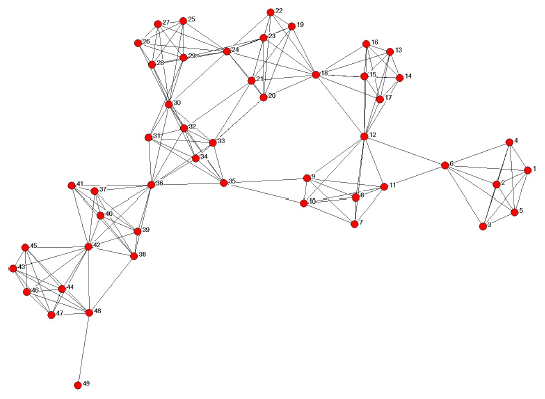
\includegraphics[width=11cm]{./imagenes/red_al_qaeda.png}
    \caption{Red social conformada por las células terroristas de Al-Qaeda.}
    \label{fig:red_al_quaeda}
  \end{center}
\end{figure}

La evolución de los servicios proporcionados a través de la internet ha sido drástica puesto que ha cambiado el modo de vida de las personas. En la figura \ref{fig:utilizacion_internet} se evidencia el crecimiento de la internet (de los servicios que en ella se soportan) se da en función de los servicios de conectividad social que son creados y soportados en ella. La web 1.0 fue utilizada en mayor medida por científicos para el intercambio de información en formato hipertexto. No había una interacción fuerte entre cada científico sino que ellos acudían a internet para buscar o poner a disposición material científico. Con la venida de la web 2.0 y la introducción de la interacción del usuario con la web generando contenido en tiempo real, así se crearon servicios de redes sociales en-línea (OSN en inglés: On-line Social Network), produciento una partición en los tipos de redes sociales. Así, las redes sociales a las que pertenece el ser humano en la era digital se dividieron convenientemente en “redes sociales fuera de línea” y redes sociales en línea (Offline Social Network y Online Social Network).

\begin{figure}[!htb]
  \begin{center}
    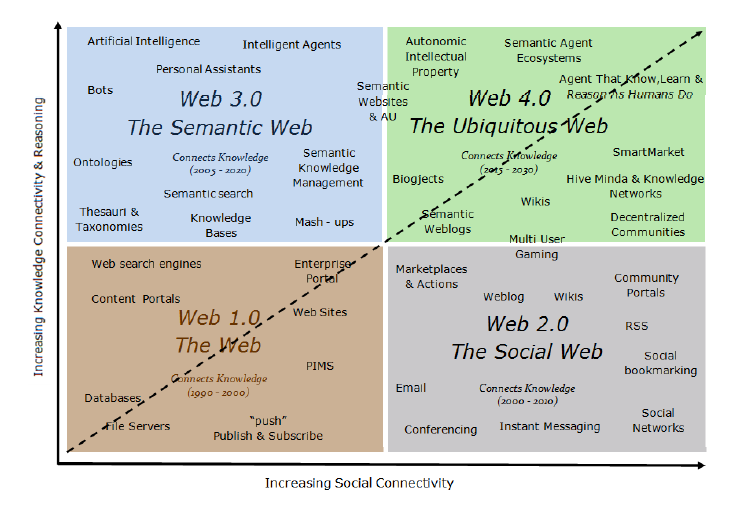
\includegraphics[width=11cm]{./imagenes/utilizacion_internet.png}
    \caption{Cambio de la utilización de internet en función de los servicios de conectividad social que son creados y soportados en ella}
    \label{fig:utilizacion_internet}
  \end{center}
\end{figure}

Las redes sociales fuera de línea son las redes sociales que se forman por comunicación tradicional (lenguaje oral y escrito en medios que difieran de aquellos que utilizan las telecomunicaciones). Las redes sociales en línea son aquellas redes sociales que están formadas por cibernautas y en las cuales la comunicación se da por medio de los servicios de redes sociales.

La administración de una red social fuera de línea fue estudiada desde inicios del siglo XX\cite{dynamics} con un enfoque socio-matemático llamado “análisis de redes sociales” (SNA por sus siglas en ingles: Social Network Analisis). Sin embargo, era difícil el análisis del comportamiento humano según los designios de la SNA puesto que la información debía ser recopilada por medio de entrevistas a las personas. Aún así, el enfoque SNA fue utilizado para analizar el comportamiento terrorista o inclusive el comportamiento de trabajadores en una empresa.\cite{sna_startups}

Con la creación de las OSN y la gran cantidad de información que describe el comportamiento humano sobre este tipo de red social, ha sido más sencillo utilizar el enfoque de la SNA para estudiar que comportamientos tienen los humanos sobre una red social establecida.

Los servicios de redes sociales (SNS por sus siglas en ingles: Social Network Services) como Facebook, LinkedIn, Twitter, SportTracker o Xportia, ofrecen servicios para la gestión de la OSN de cada usuario que acceda a estas aplicaciones. Según un estudio hecho para medir la experiencia de usuario (UX por sus siglas en ingles: User eXperience) en los SNS, se encontraron 8 categorías que son críticas a la hora de diseñar una SNS y son:

1. Self-expresion: Capacidad que tengan las OSN de compartir contenido relacionado a la vida real de los usuarios tal como lo pueden ser las fotos, los videos, los comentarios o las comunicaciones directas.
2. Reciprocity: Interacción bilateral en tiempo real, es decir, interacción instantánea con uno o varios individuales en la OSN (por ejemplo, por medio de los servicios de mensajería instantánea).
3. Learning: La información recibida por medio de la OSN debe poder ser utilizada en pro del desarrollo cognitivo del individual; debe existir información útil al individual que usa la OSN.
4. Curiosity: El contenido de la OSN debe ser interesante para quien la utiliza.
5. Suitability of functionality: Se refiere a cuán “utilizable” es una funcionalidad.
6. Suitability of content: La calidad y exactitud de la información que en la OSN reside debe ser suficiente para el individual perteneciente a ella.
7. Completeness of the user network: Los individuales deben querer pertenecer a la red social y buscar eficientemente a otros individuales para poder formar lazos con ellos y hacer crecer su red social.
8. Trust and privacy: Confianza en los servicios de las OSN, así como también la capacidad que tiene el usuario de gestionar la privacidad del contenido que comparte en dicha OSN.\cite{social_experience}

De acuerdo al enfoque SNA, las redes sociales pueden estar divididas en clusters, que no son más que agrupaciones de individuales sobre una red social por algún concepto como, por ejemplo, la pertenencia a una comunidad. Con lo anterior, podemos encontrar que algunos SNS ofrecen servicios para gestionar las OSN de sus usuarios centrándose en algún tipo de comunidad en específico y, la información que circula por ese tipo de comunidades, es diferente a la que pasa por SNS descentralizados (como Facebook y twitter). Viendo Facebook como una agrupación de clusters con temáticas tan diferentes como lo son los deportes y la música, la ciencia y la vida cotidiana, se puede decir que algunos SNS se enfocan en alguna de estas temáticas. En este caso, el cluster o temática que compete al trabajo a elaborar es el deporte.

Es posible hacer una división del cluster deporte en otros subclusters de cada uno de los deportes que existen en el mundo o en la clasificación de los deportes que han dado organizaciones como, por ejemplo, la IWGA (Internation WorldGames Association). Lo que se quiere con este trabajo es aportar al crecimiento de las redes sociales fuera de linea de las personas que practiquen deporte sin importar si lo hacen a nivel profesional o aficionado por medio de un SNS orientado a los deportes en general y, por lo tanto, el cluster que se ha escogido para trabajar es el del deporte como cluster mismo.

Se investigó acerca de las redes sociales existentes enfocadas a la temática del deporte y se encontró que muchas de ellas son utilizadas en mayor medida en España y que todas ellas están soportadas sobre tecnologías web. En general, solo se encontraron dos redes sociales deportivas orientadas a cualquier deporte asociadas a aplicaciones para smartphones disponibles en el la tienda virtual de Android o en la tienda virtual de Apple (La red social de Fitivity y Huddlers).

Así, con la evolución de la comunicación humana trasladándose a los espacios virtuales por medio de las OSN y la falta de aplicaciones, en el campo de los smartphones, que soporten interacciones sociales enfocadas a los deportes en general, en este trabajo se creará un SNS centrado en los deportes sobre tecnologías Android para la administración de las OSN de cada persona en un ámbito deportivo desde su dispositivo móvil.

  
  \chapter{Justificación del problema}
  Los humanos, desde siempre en su evolución, han necesitado de mecanismos para comunicarse con sus congéneres. En la actualidad, uno de los mecanismos es el uso de los SNS como facebook y twitter, cada uno de ellos modificando la forma de creación de redes sociales en la actualidad. (Sección \ref{sec:red})

De acuerdo al análisis egocéntrico de las redes sociales de cada individuo, se hace conveniente la utilización de SNS para gestionar las relaciones que un individuo mantiene con otros individuos (sean personas u organizaciones) en los diferentes círculos sociales en los que se mueve. (Sección \ref{sec:egocentrico})

El círculo social o comunidad escogida para el desarrollo propuesto es la comunidad deportiva debido a que hay mucha información dispersa alrededor de internet que es ambigua y a veces inclusive errónea. A su vez, debido a que gran cantidad de deportes no han tenido una acogida grande alrededor del mundo, las comunidades que se mueven sobre uno de esos deportes son más cerradas y, por ende, pequeñas y con poca información para un público que salga de las fronteras de dichas comunidades cerradas. Lo que se quiere con este trabajo es aportar al crecimiento de las redes sociales de las personas que practiquen deporte sin importar si lo hacen a nivel profesional o aficionado por medio de un SNS orientado a los deportes en general.

Un factor de utilización masiva de las SNS es que éstas estén orientadas a un público en particular y aumenten su cobertura dependiendo de su alcance de masa crítica sobre una red social definida \cite{sna_startups}. Al construir, en principio, la red social deportiva enfocada en dos deportes en particular, la probabilidad de ganar la masa crítica es mayor y, por tanto, el SNS desarrollado puede volverse más útil con el tiempo.

La UX de los SNS (visto en el capítulo \ref{cap:estado_arte}) es otro factor, debido a que juega un papel importante pues es esta la segunda carta de presentación de un SNS. Algunas de las características que evalúan los usuarios en cuanto a la UX no son suplidas por los SNS actuales – o al menos no parcialmente - , tres de ellas (fundamentales para la acogida de un nuevo SNS) son “curiosity, learning y completeness of the social network”. Así, habiendo analizado 19 SNS orientados al deporte (Tablas \ref{tab:comparacion_redes_1} a \ref{tab:comparacion_redes_5}), se concluyó que fallaban en alguna de las tres características mencionadas.

Tener en cuenta la población a quien va dirigido el SNS a desarrollar es otro factor de éxito. Según \cite{user_behavior_online}, entre los años de adolescencia y los 40 años de edad, las personas acuden con mayor interés al uso de los SNS; al ser la comunidad del deporte comprendida en su mayoría por personas entre la adolescencia y los 40 años, aumenta aún más la probabilidad de alcanzar la masa crítica y volver útil con el tiempo el SNS.

Un último factor, que se observó, afecta la creación de redes sociales (tanto fuera de línea como en línea) (Sección \ref{sec:red}) es la distancia entre cada individual y el posible tipo de enlace que los uniría. Al ver la importancia de manejar SNS que ofrezcan servicios de geolocalización, se ha visto pertinente añadir dicho servicio a la creación del prototipo de SNS orientado a los deportes en general.

También se encontró evidencia de poca utilización de los SNS que no estaban orientadas a móviles. Dichos SNS eran utilizados mucho más por personas
que practican deportes que empiezan a tomar vuelo o deportes poco conocidos (un ejemplo de ello es el padel). El problema con dichos SNS es la
naturaleza nómada de los deportistas. Una solución a la naturaleza nómada de los deportistas y el acercamiento de los últimos a las TICs y, en este caso, a
los SNS deportivos es la aparición y utilización en masa de los smartphones.

En general, solo se encontraron dos redes sociales deportivas orientadas a cualquier deporte asociadas a aplicaciones para smartphones disponibles en el la tienda virtual de Android o en la tienda virtual de Apple (La red social de Fitivity y Huddlers) (Tablas \ref{tab:comparacion_redes_1} a \ref{tab:comparacion_redes_5}). Además, hay una ventaja real en hacer una red social orientada a dispositivos móviles y es la capacidad de movilidad que ellos brindan mientras se está utilizando el servicio \cite{spiderweb}. Dada la falta de aplicaciones móviles en el campo descrito y a su vez la importancia que toman los dispositivos móviles por sus características, se ha decidido hacer el prototipo de SNS orientado al deporte sobre tecnologías móviles.

  
  \chapter{Objetivos}
  \section{Objetivo General}
   Desarrollo de un prototipo SNS (Social Networking Service) centrado en el deporte sobre tecnologías Android que permita al usuario el acceso a diferentes servicios propios de una red social que permita facilitar la comunicación y el acceso a la información a quienes son parte de la comunidad deportiva.

  \section{Objetivos específicos}
   \begin{itemize}
  \item Investigar acerca de los deportes en los que se probará el prototipo, teniendo en cuenta todo el entorno que rodea el deporte así como el deporte mismo.

  \item Investigar acerca de tecnologías utilizadas en el desarrollo de SNS y el desarrollo para móviles con el fin de determinar las herramientas a utilizar en el
desarrollo del proyecto.

  \item Analizar los diferentes SNS existentes para conocer el entorno en el que se desenvolverá el prototipo a desarrollar en el presente trabajo y, así, hacer parte
de la ayuda para definir las funcionalidades de este.

  \item Investigar acerca de la teoría de las redes sociales y de la computación orientada a servicios con el fin de que el prototipo a desarrollar esté cimentado sobre
bases teóricas sólidas.

  \item Aplicar la metodología propuesta en la computación orientada a servicios
\end{itemize}


  \chapter{Marco conceptual}
  A continuación, se definen algunos conceptos que intervienen con el desarrollo del presente proyecto.

\section{Comunicación}

Los científicos han estudiado el porqué de las relaciones complejas entre los humanos en comparación a la complejidad presentada en las relaciones entre otros animales. Una de las hipótesis, Social Brain Hypothesis (SBH) postula que el crecimiento cognitivo humano y sus intrincadas relaciones sociales se deben a “la necesidad de nuestros ancestros de mantener e incrementar el número de relaciones sociales con diferentes grupos para sobrevivir en las extremadamente desafiantes condiciones ambientales originadas durante la última era glacial”.\cite{dynamics}

El hombre, en su continua evolución, ha utilizado el lenguaje como una herramienta creadora de conocimiento transferible a sus congéneres o cualquier otro ser que interactuase con él. Con esto, “los humanos han desarrollado el lenguaje como un instrumento ligero y conveniente para mantener sus relaciones” \cite{dynamics}. 

En la comunicación entre congéneres, el lenguaje puede ser dividido en dos funciones: función de transmisión de información (gossip) y función de entendimiento del estado interno (estado mental) del congénere (mentalisation) \cite{dynamics}. Estas funciones de transmisión y entendimiento del otro han permitido que dos o varios humanos puedan asociarse entre sí formando redes sociales.


\subsection{Evolución de la web}

La evolución de los servicios proporcionados a través de internet ha sido drástica puesto que ha cambiado el modo de vida de las personas. En la figura \ref{fig:utilizacion_internet} se evidencia que el crecimiento de internet (de los servicios que en ella se soportan) se da en función de los servicios de conectividad social que son creados y soportados en ella. La web 1.0 fue utilizada en mayor medida por científicos para el intercambio de información en formato hipertexto. No había una interacción fuerte entre cada científico sino que ellos acudían a internet para buscar o poner a disposición material científico. Con la venida de la web 2.0 y la introducción de la interacción del usuario con la web, generando contenido en tiempo real, fueron creados servicios de redes sociales en-línea (OSN en inglés: On-line Social Network), produciendo una partición en los tipos de redes sociales. Así, las redes sociales a las que pertenece el ser humano en la era digital se dividieron convenientemente en “redes sociales fuera de línea” y “redes sociales en línea” (Offline Social Network y Online Social Network) \cite{dynamics}.

\begin{figure}[!htb]
  \begin{center}
    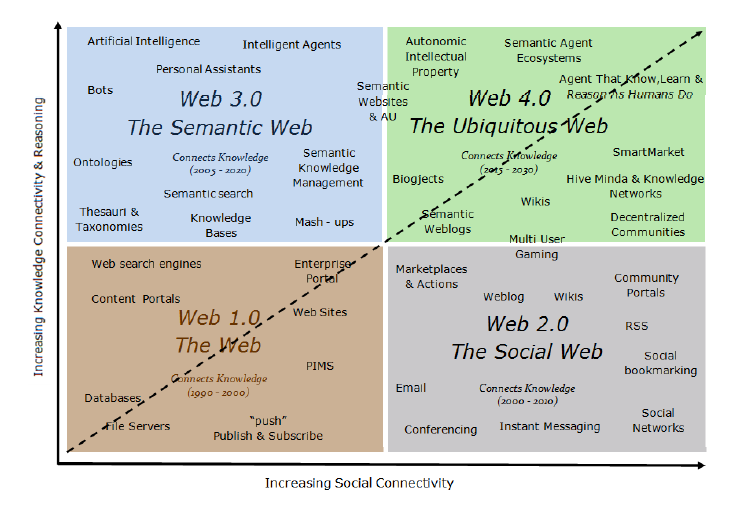
\includegraphics[width=11cm]{./imagenes/utilizacion_internet.png}
    \caption{Cambio de la utilización de internet en función de los servicios de conectividad social que son creados y soportados en ella}
    \label{fig:utilizacion_internet}
    \textbf{Fuente:}  http://goo.gl/3jGPPJ - Evolución de la web. Lozada, Pablo.
  \end{center}
\end{figure}


\section{Réd social}

La información contenida en la actual sección es tomada del libro \textit{Social Network Analisis for Startups} \cite{sna_startups}

Una red es un conjunto de relaciones. Mas específicamente, una red consiste en un conjunto de objetos (nodos) que están interconectados a través de relaciones (aristas). La red mas simple consiste en 2 nodos, N1 y N2, que están relacionados entre sí (Figura \ref{fig:simple}). Los nodos podrían representar personas, mientras la arista representa la relación que existe entre ellas (N1 y N2 son amigos, por ejemplo).

\begin{figure}[!htb]
  \begin{center}
    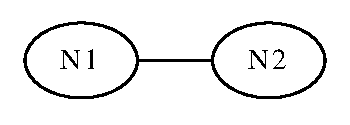
\includegraphics{./imagenes/Red_simple.eps}
    \caption{La red mas simple.}
    \label{fig:simple}
    \textbf{Fuente:}  Autores
  \end{center}
\end{figure}

Las redes sociales fuera de línea son las redes sociales que se forman por comunicación tradicional (lenguaje oral y escrito en medios que difieran de aquellos que utilizan las telecomunicaciones). Las redes sociales en línea son aquellas redes sociales que están formadas por cibernautas y en las cuales la comunicación se da por medio de los servicios de redes sociales. \cite{analysis}

Las relaciones pueden ser simétricas o asimétricas. Cuando se tiene una relación simétrica se dice que la relación no tiene dirección, es decir, la relación puede leerse en ambos sentidos. En el ejemplo anterior, significaría que N1 es amigo de N2 y que N2 es amigo de N1. Para que una relación se considere asimétrica, la relación debe poder leerse en un único sentido, es decir, la relación tiene una dirección determinada. En la figura \ref{fig:asimetrica} se puede observar un ejemplo de una red asimétrica en donde el nodo (o persona) N1 sigue al nodo N2, pero el nodo N2 no sigue al nodo N1.

\begin{figure}[!htb]
  \begin{center}
    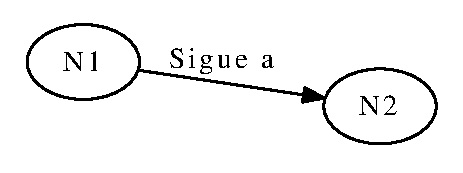
\includegraphics{./imagenes/Red_asimetrica.eps}
    \caption{Ejemplo de una red asimétrica.}
    \label{fig:asimetrica}
    \textbf{Fuente:}  Autores
  \end{center}
\end{figure}

Es posible que exista mas de una relación entre 2 nodos, en ese caso se dice que existe una \textit{relación multiplex} \cite[Cap.2]{cap_sna}


\section{Business Process Modeling Notation (BPMN)}

La información contenida en la actual sección es tomada del libro \textit{BPMN 2.0 Introduction to the Standard for Business Process Modeling} \cite{bpmn2}

Al interior de una organización es importante documentar y especificar los diferentes procesos que se deben llevar a cabo. A menudo, se suelen utilizar diagramas de flujo o incluso descripciones textuales. Desafortunadamente, estas técnicas se quedan cortas a la hora de describir procesos mas complejos, y mas aún cuando cada organización define su propia notación, dificultando el entendimiento de los diferentes modelos que se realizan al interior de la organización. Es por esto que se hace necesario crear una notación estándar y especifica para describir este tipo de procesos.

BPMN, Business Process Modeling Notation, es precisamente el estándar que se viene adoptando a nivel masivo para la creación y descripción de los diferentes procesos que hacen parte del funcionamiento de las diferentes organizaciones.


Con el estándar BPMN, se tienen en cuenta diferentes elementos básicos que sirven como herramientas para crear y estructurar los diferentes modelos que se quieran hacer. Estos elementos solo describen una forma básica de uso, pues BPMN permite personalizar los elementos a utilizar, siempre y cuando los cambios realizados no dificulten el proceso de entendimiento de los modelos.

\subsection{Pertinencia con el proyecto}

Se utilizará BPMN como ayuda para el modelamiento de los diferentes procesos de negocio que sean identificados en la fase de análisis. Esto facilitará el proceso de diseño e implementación de los diferentes componentes necesarios para dar solución a los diferentes requerimientos del negocio.

\section{Service-Oriented Architecture (SOA)}

La información contenida en la actual sección es tomada del libro \textit{Soa principles of service design} \cite{soa_principles}

\subsection{Primeros conceptos}

Los conceptos base del diseño de software deben ser expuestos para tener una mayor claridad en los temas siguientes. A continuación se expresan los conceptos base:

\begin{itemize}
  \item \textbf{Características de diseño}: Son aquellos atributos que cumple un diseño y que pueden ser medidos.
  \item \textbf{Principio de diseño}: Es una guía o regla para solucionar un problema de acuerdo a las prácticas aceptadas por la comunidad de ingeniería de software.
  \item \textbf{Paradigma de diseño}: Es el compendio de principios de diseño que tienen un enfoque global común.
  \item \textbf{Patrones de diseño}: Son formas de resolver un problema de diseño que es repetitivo. Viene dado por 3 restricciones presentadas en el diseño de software:
  \begin{itemize}
    \item Restricciones impuestas por la tecnología existente
    \item Restricciones impuestas por las tecnologías usadas por sistemas transversales
    \item Restricciones de prioridades de proyectos
  \end{itemize}
  El patrón de diseño describe el problema y da la solución a modo de plantilla.
  \item \textbf{Lenguajes de patrones de diseño}: Es la configuración ordenada de patrones en un diseño lógico. La comunicación entre cada patrón se hace a través de dicho lenguaje.
  \item \textbf{Estándares de diseño}: En orden de ir acorde a las metas, prioridades, recursos y ambiente de la organización en la que se haga el diseño lógico de la solución, un estándar de diseño define convenciones para cada elemento utilizado en el diseño de acuerdo a las características de diseño definidas.
  \item \textbf{Buenas prácticas}: Es una técnica o acercamiento para resolver o prevenir problemas presentados en el desarrollo del diseño lógico de la solución de software. pg 34
\end{itemize}

\begin{figure}[!htb]
  \begin{center}
    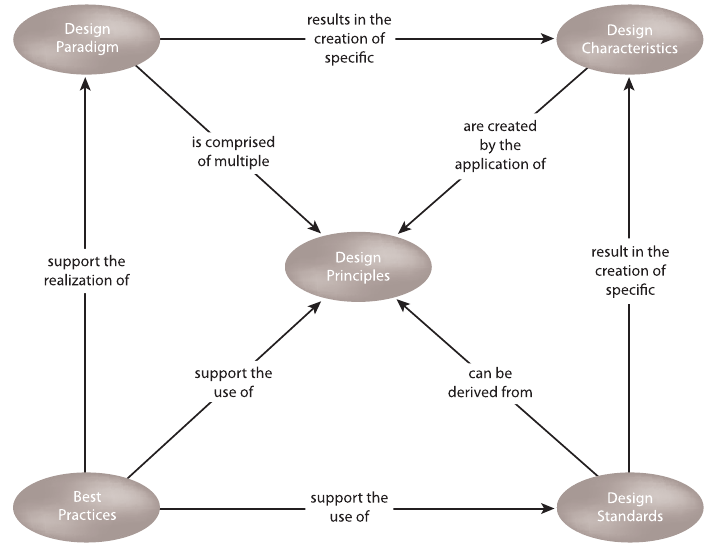
\includegraphics[width=11cm]{./imagenes/1.png}
    \caption{Acercamiento a cómo se desarrollan los principios de diseño con los demás conceptos nombrados.}
    \label{fig:uno}
    \textbf{Fuente:}  \cite{soa_principles}
  \end{center}
\end{figure}

La figura \ref{fig:uno} presenta un acercamiento a cómo se desarrollan los principios de diseño con los demás conceptos nombrados.

\begin{figure}[!htb]
  \begin{center}
    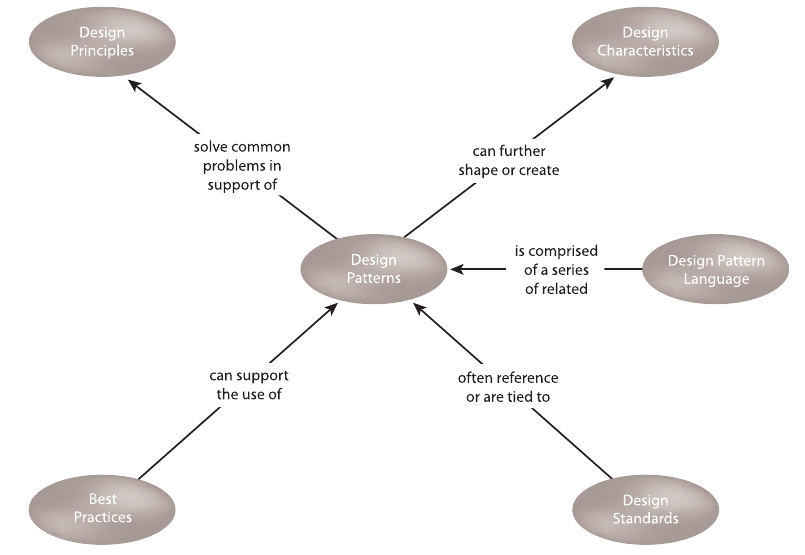
\includegraphics[width=11cm]{./imagenes/2.png}
    \caption{Como extiende o soporta un patrón de diseño el diseño lógico de la solución de software.}
    \label{fig:dos}
    \textbf{Fuente:}  \cite{soa_principles}
  \end{center}
\end{figure}

La figura \ref{fig:dos} presenta cómo extiende o soporta un patrón de diseño el diseño lógico de la solución de software.

\begin{figure}[!htb]
  \begin{center}
    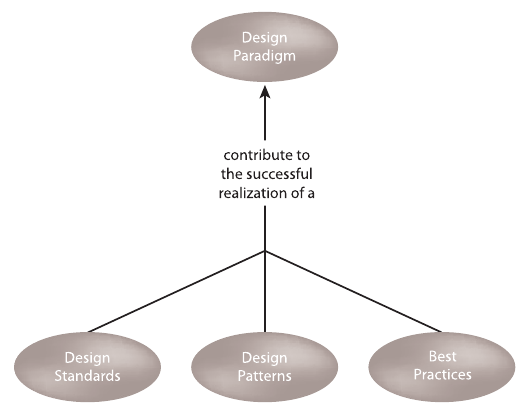
\includegraphics[width=11cm]{./imagenes/3.png}
    \caption{Componentes que hacen que el diseño lógico de la solución sea acorde al paradigma escogido.}
    \label{fig:tres}
    \textbf{Fuente:}  \cite{soa_principles}
  \end{center}
\end{figure}

La figura \ref{fig:tres} presenta los componentes que hacen que el diseño lógico de la solución sea acorde al paradigma escogido.

\subsection{Computación orientada a servicios}

La computación orientada a servicios nace de la necesidad de desarrollar software integrado con otros construidos con diferentes arquitecturas y, por ende, diversas tecnologías. Este tipo de computación tiene como finalidad la construcción de inventarios de servicios. La computación orientada a servicios está compuesta por la interacción de la orientación a servicios (paradigma de diseño) y la arquitectura orientada a servicios, formando patrones de diseño propios y estándares en cumplimiento de las características de diseño propias de la computación orientada a servicios. 

Algunos de los conceptos clave llevados en la computación orientada a servicios son:

\begin{itemize}
  \item Arquitectura Orientada a Servicios (SOA - Service Oriented Architecture): Comprende el compendio de tecnologías, APIs, infraestructura y repositorios enmarcados en el paradigma orientado a servicios y cuyo objetivo principal es el de trabajar sobre el "servicio" como el elemento más importante.
  \item Orientación a servicios: Es el paradigma manejado en la computación orientada a servicios en donde se acepta como unidad mínima y más importante el "servicio".
  \item Servicio: Es un software independiente físicamente el cual tiene asignado un contexto de funcionalidades y que puede ser utilizado por otros servicios por medio del contrato del servicio (descripción del servicio en cuanto a funcionalidades, entradas requeridas y salidas). De acuerdo a su nivel de reúso, los servicios se dividen en 3 tipos y son:
  \begin{itemize}
    \item Servicios entidad: Modela los servicios que se deben ofrecer respecto de las entidades del negocio (ej. empleados y clientes). Tienen un nivel de reúso alto y están centrados en el negocio.
    \item Servicios tarea: Modela los servicios que deben cumplir tareas específicas del negocio (ej. generación de cortes de final de año). Tienen un nivel de reúso bajo. Estos servicios trabajan directamente con 1 o varios servicios entidad. Estos servicios están centrados en el negocio.
    \item Servicios utilidad: Modela servicios que no están centrados en el negocio. Son los servicios con mayor reúso.
  \end{itemize}
\end{itemize}

\begin{figure}[!htb]
  \begin{center}
    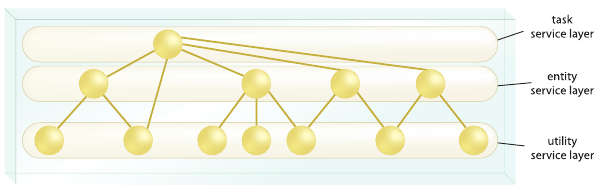
\includegraphics[width=11cm]{./imagenes/5.png}
    \caption{diferenciación entre tipos de servicio da lugar a la estructura en capas}
    \label{fig:cinco}
    \textbf{Fuente:}  \cite{soa_principles}
  \end{center}
\end{figure}

La diferenciación entre tipos de servicio da lugar a la estructura en capas mostrada en la figura \ref{fig:cinco}

\begin{itemize}
  \item Composición de servicios: Es la agregación de servicios de manera ordenada.
  \item Inventario de servicios: Es la agrupación de varios servicios según un criterio definido por la organización. Cada inventario de servicios tiene su propio estándar de diseño e, inclusive, su propia configuración arquitectónica. El desarrollo de los inventarios de servicio es hecho a modo top-down, con la construcción de blueprints, también llamados modelo de servicios de negocio o modelos de inventario de servicios.
\end{itemize}

\begin{figure}[!htb]
  \begin{center}
    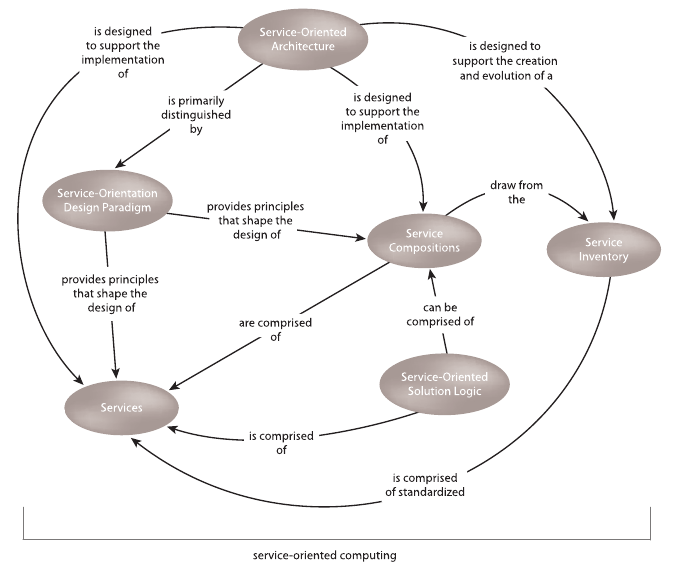
\includegraphics[width=11cm]{./imagenes/4.png}
    \caption{Interacción de los conceptos clave en la computación orientada a servicios}
    \label{fig:cuatro}
    \textbf{Fuente:}  \cite{soa_principles}
  \end{center}
\end{figure}

\subsection{Pertinencia con el proyecto}


La arquitectura base para la ejecución del proyecto es SOA. Esto brinda diferentes beneficios a la hora del desarrollo del proyecto, como los son:
\begin{itemize}
  \item Gracias al bajo acoplamiento conseguido con la arquitectura SOA, los componentes implementados son altamente reutilizables, lo que facilita y agiliza el proceso de desarrollo. Ademas,
  \item Es posible consumir servicios creados por terceros, limitando los servicios que deben ser creados a los que sean estrictamente de negocio.
\end{itemize}

\section{Scrum}

Sus creadores lo describen como “Un marco de trabajo por el cual las personas pueden acometer problemas complejos 
adaptativos, a la vez que entregar productos del máximo valor posible productiva y creativamente” \cite{scrum_guide}. Scrum se caracteriza por ser ágil, ligero, fácil de entender y difícil de llegar a dominar.

Scrum se basa en el empirismo, que dice que el conocimiento proviene de la experiencia, por lo que ``utiliza un enfoque iterativo e incremental para optimizar la predictibilidad y el control del riesgo'' \cite{scrum_guide}.

Los tres grandes pilares de la teoría de scrum son:

\begin{itemize}
  \item Transparencia: Todos los aspectos significativos deben ser visibles para sus stakeholders respectivos.

  \item Inspección: Los artefactos de scrum (y su progreso) deben ser inspeccionados frecuentemente para detectar variaciones. Estas inspecciones deben ser realizadas por un experto.

  \item Adaptación: Cuando una inspección detecta una variación que no cae en los limites permitidos, se deben hacer los reajustes necesarios para que el producto vuelva a rumbo deseado. Estos cambios deben hacerse lo más pronto posible, por esto las inspecciones deben ser realizadas de manera periódica a lo largo del desarrollo del proyecto.
\end{itemize}

 
  \chapter{Marco teórico}
  \section{Redes Sociales} \label{sec:red}

La información contenida en la actual sección es tomada del libro \textit{Social Network Analisis for Startups} \cite{sna_startups}

\subsection{SNA: Social Network Analisis}

La administración de una red social fuera de línea fue estudiada desde inicios del siglo XX \cite{dynamics} con un enfoque socio-matemático llamado “análisis de redes sociales” (SNA por sus siglas en inglés: Social Network Analisis). Sin embargo, era difícil el análisis del comportamiento humano según los designios de la SNA, puesto que la información debía ser recopilada por medio de entrevistas a las personas. Aun así, el enfoque SNA fue utilizado para analizar el comportamiento terrorista o inclusive el comportamiento de trabajadores en una empresa. \cite{sna_startups}

\subsection{Analisis egocéntrico} \label{sec:egocentrico}

Los estudios basados en SNA pueden ser de tipo egocéntrico o sociocéntrico \cite{user_behavior}. En los estudios egocéntricos de una red social, se analiza un individual dentro de una red social y todas las conexiones de éste hacia otros individuales en la red social analizada. El individual analizado es llamado “ego” y los individuales que hacen conexión con él son llamados “alters”. Se han identificado 4 capas en el estudio de las redes egocéntricas, estas son:

\begin{itemize}
  \item Support clique: En esta capa se identifican los alters con los que el ego hace más contacto por alguna razón de peso para él (e.g. para obtener soporte emocional). Esta capa tiene, en promedio, 5 alters.
  \item Sympathy group: En promedio a éste corresponden 15 alters.
  \item Affinity group: En promedio a éste corresponden 50 alters.
  \item Active network: En promedio a éste corresponden 150 alters.
\end{itemize}

Los números dados en las capas descritas en el análisis egocéntrico son congruentes con el número de Dunbar, el cual representa el umbral promedio de número de alters sobre la capa “active network” (150) según Robin Dunbar, argumentando que este límite se debe a la capacidad cognitiva del cerebro humano \cite[Pag. 3]{dynamics} (como más adelante será nombrado, los servicios de redes sociales ayudan al ser humano a gestionar su active network, proporcionando herramientas que, en teoría y de acuerdo a la brecha tecnológica, lo ayudarán a mantener sus lazos con los alters de su red ego).

El análisis egocéntrico permite conocer los factores que dirigen al ego a crear vínculos débiles o fuertes con potenciales alters, albergándolos en alguna de las cuatro capas o en ninguna.

Con la creación de las OSN y la gran cantidad de información que describe el comportamiento humano sobre este tipo de red social, ha sido más sencillo utilizar el enfoque de la SNA para estudiar que comportamientos tienen los humanos sobre una red social establecida.

\subsection{Grado de centralidad}

En todas las redes, sean virtuales o no, existen personas que son mas ``importantes'' que otras, más \textbf{populares}. Estas celebridades representan una parte muy pequeña de la red, pero debido a su gran influencia siempre es bueno identificarlos. Para esto se utiliza el \textbf{grado de centralidad}.

El grado de un nodo es la cantidad de conexiones que posee. En una red social, esto se representa por medio de las relaciones que cada nodo tenga, y ya que el significado de la relación varía en función de cada red, es necesario entender que significan las posibles relaciones existentes en una red para hacer el análisis correspondiente. Por ejemplo, en una red como Twitter en donde las relaciones son unidireccionales, puede existir un nodo con un grado de salida muy alto, esto es una persona que sigue a muchas otras. Aunque esta persona tenga un grado de centralidad muy alto, no representa una celebridad, sin embargo, un nodo que tenga un grado de entrada muy alto, que es seguido por muchas personas, si representa una persona que es muy popular en esta red.

\begin{figure}[!htb]
  \begin{center}
    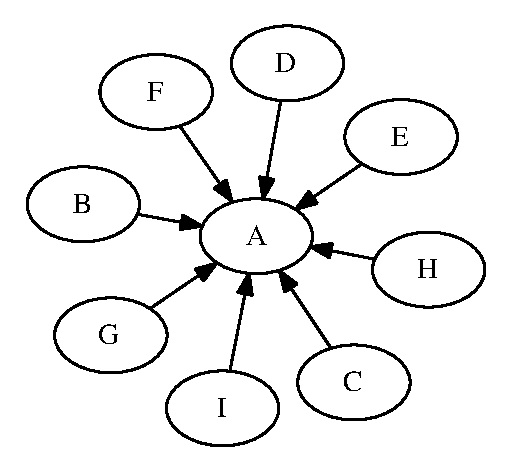
\includegraphics{./imagenes/red_estrella.eps}
    \caption{Red de estrella.}
    \label{fig:red_estrella}
    \textbf{Fuente:}  Autores
  \end{center}
\end{figure}


En la figura \ref{fig:red_estrella} se puede ver un caso en el que el nodo A es una clara celebridad de la red. Este tipo de configuración, llamada red de estrella, es muy poco común en la vida real, pero sirve de ayuda visual para entender a simple vista el concepto de centralidad.

\subsection{Grado de cercanía}

A menudo se puede ver que personas que no tienen mayor influencia aparente en una red son capaces de difundir un mensaje en una gran parte de la red. Esto se debe a que tienen buenas conexiones en la red que les permiten llegar a mas personas, sin que ellos en si sean ``importantes'' en la red. Para medir que tan bien o mal posicionado esta un nodo en la red se utiliza el \textbf{grado de cercanía}. Este calculo es bastante caro computacionalmente ya que conlleva una gran cantidad de cálculos.

Los pasos para calcular el grado de cercanía de los nodos de una red son:

\begin{enumerate}
  \item Calcular la ruta mas corta entre todos los pares de nodos posibles, utilizando el algoritmo de Dijkstra, y almacenar estos valores en una tabla.
  \item Para cada nodo de la red:
  \begin{enumerate}
    \item Calcular la distancia promedio con todos los demás nodos.
    \item Dividir el promedio por la distancia mas alta.
    \item Calcular el inverso del valor anterior.
  \end{enumerate}
  \item normalizar cada valor obtenido para obtener valores en el rango de 0-1.
\end{enumerate}

Los nodos que tengan un valor mas cercano a 1 son los que tienen una distancia promedio menor con los nodos de la red, o los que tienen ``\textit{mejores contactos}''.

\subsection{Factor distancia en la formación de las redes sociales}

La formación de redes sociales (tanto fuera de línea como en línea) es afecta por la distancia entre cada individual y el posible tipo de enlace que los uniría. En \cite{evolution} se hizo un estudio acerca de la formación de lazos, la formación de triadas entre individuales de una red social basada en la inscripción localizaciones recomendadas y frecuentadas por los usuarios, teniendo como parámetros ``la edad'' o tiempo de vinculación del individual a la red social, el grado de cada individual (número de conexiones que tiene un individual a otro) y la localización de cada individual en la red social. También se analizó cómo afectaba la creación de nuevos lazos con la movilidad del usuario (el desplazamiento por lugares geográficos distintos). En conclusión, se verificó que la formación de lazos depende proporcionalmente de la edad y del grado del individual y es inversamente proporcional a la distancia que a cada individual y que la formación de lazos puede modelarse con solo dos de los tres factores (el grado y la distancia); en cuanto a la formación de triadas, se verificó que ésta depende de las características sociales de la red, tomando énfasis en los individuales compartidos entre los posibles individuales formadores de triadas. Además, en cuanto a la creación de nuevos lazos teniendo en cuenta los lugares visitados por cada usuario de la red social, se presenta un patrón: Los usuarios escogen un lugar popular para visitar y, posteriormente, dirimen con que usuario crear un lazo teniendo en cuenta su popularidad y que frecuente los mismos lugares siempre.

\subsection{Grado de intermediación}

En las redes sociales, suelen formarse grupos mas pequeños que comparten un interés común. Por ejemplo, es mas probable que dos personas que comparten el gusto por los videojuegos interactúen entre si que dos personas que no lo hagan, sin embargo hay casos en los que una persona comparte gustos con diferentes grupos, ayudando a que esta persona se pueda relacionar de manera efectiva con un grupo mas extenso de personas. Estas personas son conocidas como ``puertas frontera'' ya que, gracias a ellos, es posible que dos grupos que no tengan nada en común puedan relacionarse entre sí. La medida que ayuda a identificar estos elementos en una red es el \textbf{grado de intermediación}, y consiste en lo siguiente:

\begin{enumerate}
  \item Calcular la ruta mas corta entre todos los pares de nodos posibles, utilizando el algoritmo de Dijkstra, y almacenar estos valores en una tabla.
  \item Para cada nodo n de la red, contar las veces que el nodo n aparece en la lista de rutas mas cortas,
  \item normalizar cada valor obtenido para obtener valores en el rango de 0-1.
\end{enumerate}

Cabe notar que este algoritmo es bastante lento para redes que son muy grandes.

En la figura \ref{fig:bow_tie} se puede ver un claro ejemplo de este fenómeno. Esta red, comúnmente denominada la "red corbatín" gracias a su forma similar a la de un corbatín, muestra como el nodo D se encuentra entre 2 grupos de nodos que, de otra manera, no podrían conectarse.

\begin{figure}[!htb]
  \begin{center}
    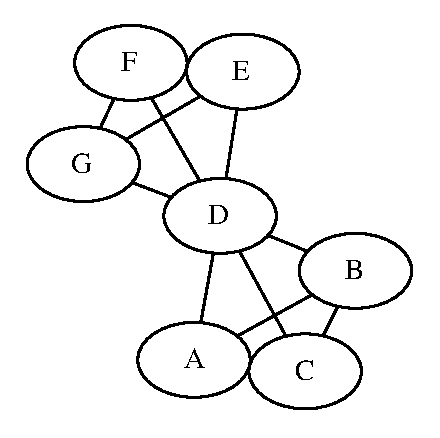
\includegraphics{./imagenes/bow_tie.eps}
    \caption{red corbatín.}
    \label{fig:bow_tie}
    \textbf{Fuente:}  Autores
  \end{center}
\end{figure}

\subsection{Díadas}

Las díadas son la unidad básica de análisis una red social, ya que estas representan la relación entre una y otra persona, esto es, mis amigos, mis seguidores, mis suscriptores, etc. Existen 4 tipos de díadas, representadas en la figura \ref{fig:tipos_diadas}, su uso varia en función del significado de la relación.

\begin{figure}[!htb]
  \begin{center}
      \begin{tabular}{m{3cm}|m{3cm}|m{3cm}|m{3cm}}
        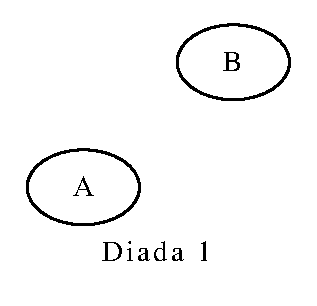
\includegraphics[width=3cm]{./imagenes/diada_1.eps} & 
        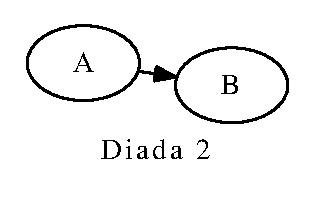
\includegraphics[width=3cm]{./imagenes/diada_2.eps} & 
        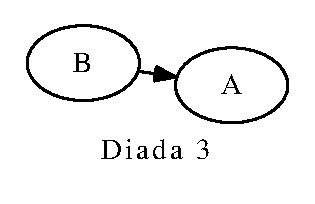
\includegraphics[width=3cm]{./imagenes/diada_3.eps} & 
        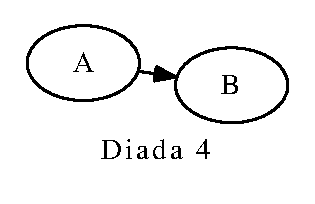
\includegraphics[width=3cm]{./imagenes/diada_4.eps}\\
      \end{tabular}
    \caption{Tipos de diadas asimétricas.}
    \label{fig:tipos_diadas}
    \textbf{Fuente:}  Autores
  \end{center}
\end{figure}


La díada 1 indica que ambos individuos existen en la red, pero todavía no existe ninguna relación entre ellos. Las diadas 2 y 3 muestran una relación unidireccional entre los dos individuos, la única diferencia es el sentido de esa relación. La díada 4, por su parte, es la de mayor interés de las cuatro ya que muestra una relación bidireccional entre los individuos, siendo esta la relación que mayor peso tiene en una red social dado que nos dice que existe un alto grado de reciprocidad en el intercambio de información entra ambos individuos.

\subsection{Tríadas}

Las triadas son básicamente 3 nodos conectados de alguna manera. Al igual que con las diadas, las triadas también pueden ser simétricas o asimétricas, dependiendo estrictamente del contexto en que son utilizadas. Existen 4 tipos de triadas simétricas, ilustradas en la figura \ref{fig:tipos_triadas_simetricas}.

\begin{figure}[!htb]
  \begin{center}
      \begin{tabular}{m{3cm}|m{3cm}|m{3cm}|m{3cm}}
        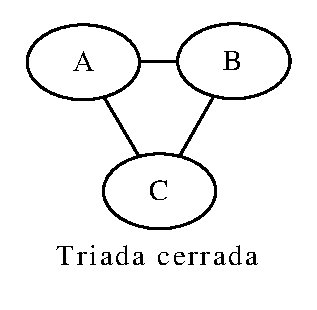
\includegraphics[width=3cm]{./imagenes/triada_simetrica_1.eps} & 
        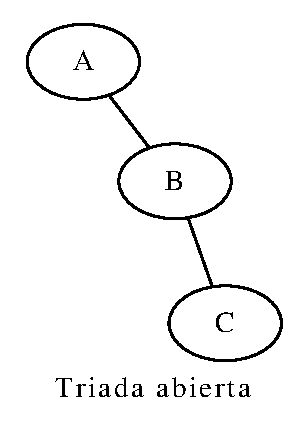
\includegraphics[width=3cm]{./imagenes/triada_simetrica_2.eps} & 
        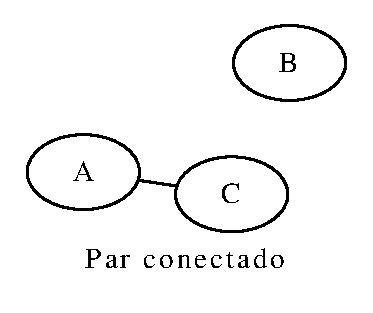
\includegraphics[width=3cm]{./imagenes/triada_simetrica_3.eps} & 
        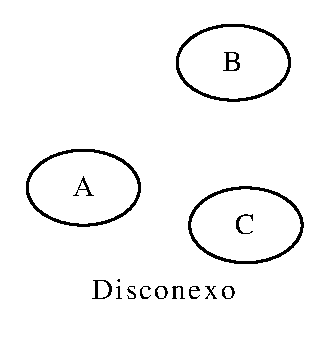
\includegraphics[width=3cm]{./imagenes/triada_simetrica_4.eps}\\
      \end{tabular}
    \caption{Tipos de triadas simétricas.}
    \label{fig:tipos_triadas_simetricas}
    \textbf{Fuente:}  Autores
  \end{center}
\end{figure}


Por otra parte, existen 16 tipos de triadas asimétricas, numeradas del 1-16. Su uso es mas frecuente ya que de ellas se puede hacer un análisis mas complejo en comparación a las díadas. Cada una de estas triadas recibe un nombre especifico para facilitar su identificación, a continuación se explica como debe leerse ese nombre:

\begin{itemize}
  \item El primer numero representa la cantidad de vértices bidireccionales
  \item El segundo numero representa la cantidad de vértices simples
  \item El tercer numero representa la cantidad de vértices inexistentes
  \item Si una triada se repite, se utiliza una letra extra para determinar que variante es:
  \begin{itemize}
    \item U - Arriba (Up)
    \item D - Abajo (Down)
    \item C - Circulo (Circle)
    \item T - Transitiva (Transitive)
  \end{itemize}
\end{itemize}

En la figura \ref{fig:tipos_triadas_asimetricas} se muestran todas las triadas posibles con su respectivo código asociado.

\begin{figure}[!htb]
  \begin{center}
      \begin{tabular}{m{1.3cm}|m{1.3cm}|m{1.3cm}|m{1.3cm}|m{1.3cm}|m{1.3cm}|m{1.3cm}|m{1.3cm}}
        \includegraphics[width=1.3cm]{./imagenes/triada_003.eps} & 
        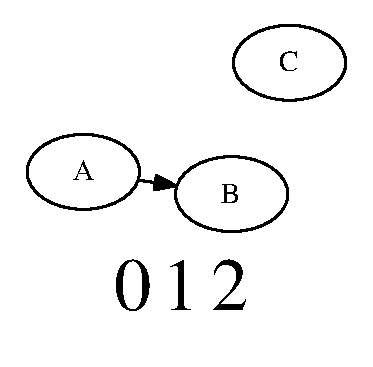
\includegraphics[width=1.3cm]{./imagenes/triada_012.eps} & 
        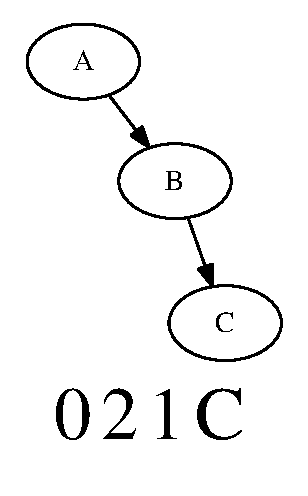
\includegraphics[width=1.3cm]{./imagenes/triada_021C.eps} & 
        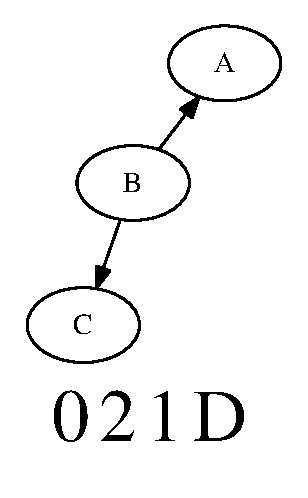
\includegraphics[width=1.3cm]{./imagenes/triada_021D.eps} & 
        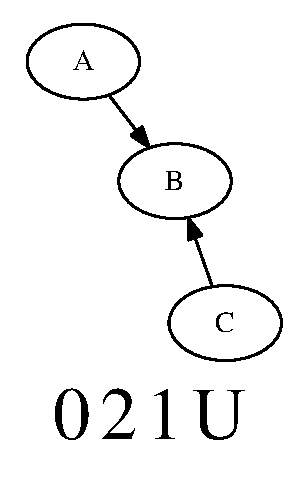
\includegraphics[width=1.3cm]{./imagenes/triada_021U.eps} & 
        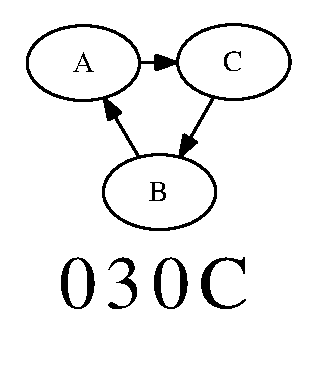
\includegraphics[width=1.3cm]{./imagenes/triada_030C.eps} & 
        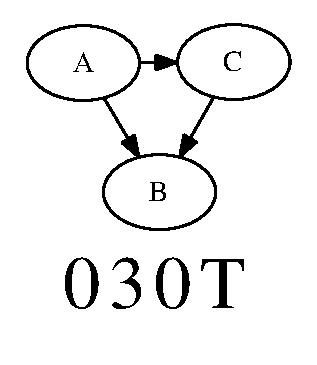
\includegraphics[width=1.3cm]{./imagenes/triada_030T.eps} & 
        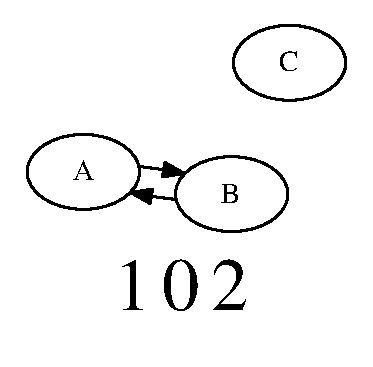
\includegraphics[width=1.3cm]{./imagenes/triada_102.eps}\\ \hline
        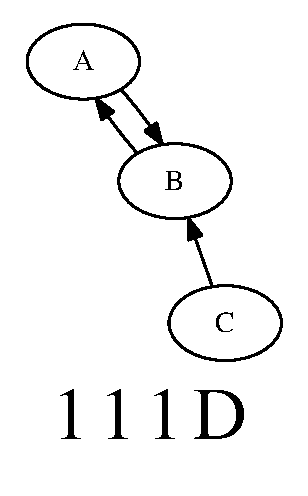
\includegraphics[width=1.3cm]{./imagenes/triada_111D.eps} & 
        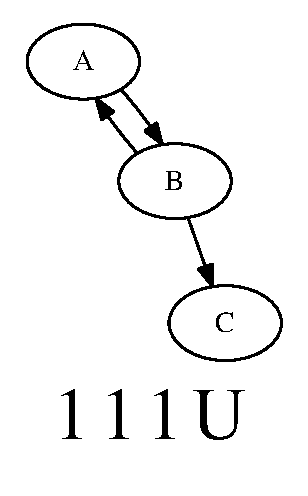
\includegraphics[width=1.3cm]{./imagenes/triada_111U.eps} & 
        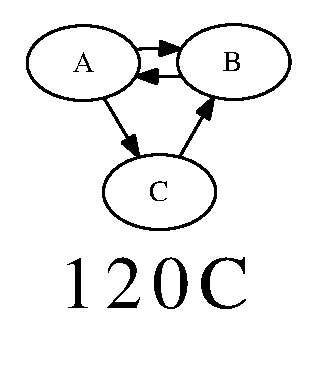
\includegraphics[width=1.3cm]{./imagenes/triada_120C.eps} & 
        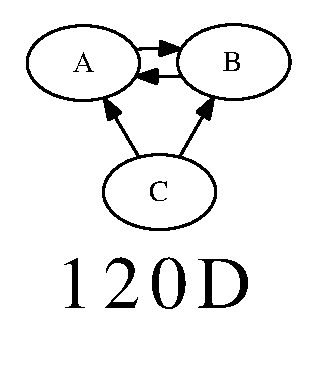
\includegraphics[width=1.3cm]{./imagenes/triada_120D.eps} & 
        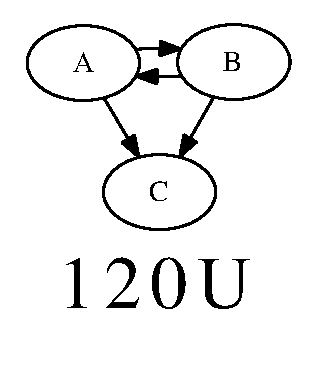
\includegraphics[width=1.3cm]{./imagenes/triada_120U.eps} & 
        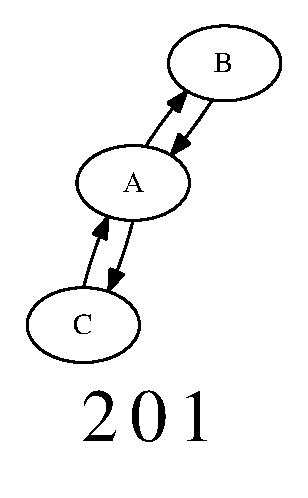
\includegraphics[width=1.3cm]{./imagenes/triada_201.eps} & 
        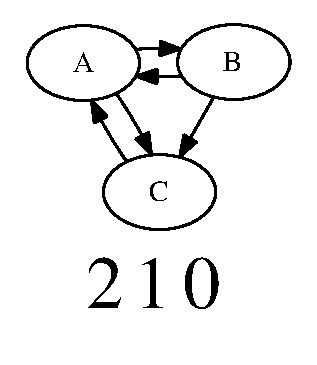
\includegraphics[width=1.3cm]{./imagenes/triada_210.eps} & 
        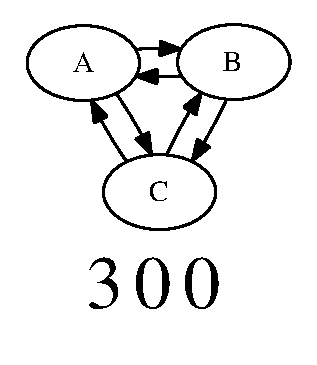
\includegraphics[width=1.3cm]{./imagenes/triada_300.eps}\\
      \end{tabular}
    \caption{Tipos de triadas asimétricas.}
    \label{fig:tipos_triadas_asimetricas}
    \textbf{Fuente:}  Autores
  \end{center}
\end{figure}


Gracias a esta discriminación topológica, se puede hacer un análisis mas completo de una red. Este análisis recibe el nombre de \textbf{\textit{Análisis Triadico}}.

\subsection{Análisis Triádico}

Este proceso, que también recibe el nombre de \textbf{Censo Triadico}, consiste en contar la ocurrencia de cada uno de los tipos de triada para cada nodo, y de esa forma determinar el rol que desempeña este nodo en la red. Por ejemplo, un nodo que presente en mayoría triadas del tipo 4, 7 y 11 es un nodo que \textbf{genera contenido}, mientras que si la mayoría de sus triadas son del tipo 5 y/o 10, es un nodo que recibe o \textbf{consume contenidos}.

Adicionalmente se puede hacer el mismo análisis a la red en general, para tener un punto de vista global de la red. En la figura \ref{fig:red_krackhardt} se puede ver una de las redes mas utilizadas en la teoría de redes sociales, la red de Krackhardt-kite. En esta red se pueden ver muchas características de una red social, facilitando el estudio de las mismas. Al hacer el censo a esta red, nos damos cuenta que presenta una gran cantidad de nodos tipo 201, que representan un agujero estructural, y nodos tipo 300, que representan triadas cerradas, esto nos indica que en esta red existen zonas que tienen una gran concentración de nodos interconectados, mientras hay zonas que no se encuentran muy pobladas. Todo esto se puede ver a simple vista en esta red, pero para redes mas grandes puede que represente un problema mayor.

\begin{figure}[!htb]
  \begin{center}
    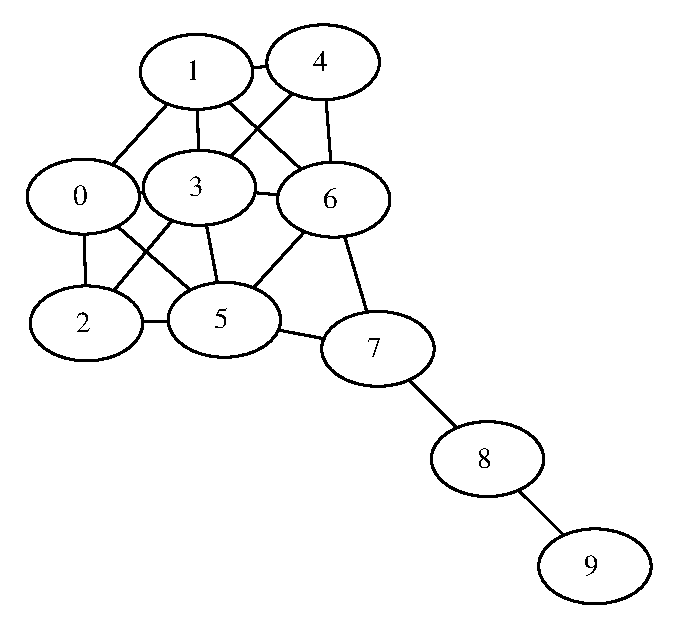
\includegraphics[width=8cm]{./imagenes/red_krackhardt_kite.eps}
    \caption{Red social de Krackhardt kite.}
    \label{fig:red_krackhardt}
    \textbf{Fuente:}  Autores
  \end{center}
\end{figure}



\section{UX - Análisis} \label{sec:UX}
Los servicios de redes sociales (SNS por sus siglas en ingles: Social Network Services) como Facebook, LinkedIn, Twitter, SportTracker o Xportia, ofrecen servicios para la gestión de la OSN de cada usuario que acceda a estas aplicaciones. Según un estudio hecho para medir la experiencia de usuario \cite{user_behavior_online} (UX por sus siglas en ingles: User eXperience) en los SNS, se encontraron 8 categorías que son críticas a la hora de diseñar una SNS y son:

\begin{enumerate}
  \item Self-expresion: Capacidad que tengan las OSN de compartir contenido relacionado a la vida real de los usuarios tal como lo pueden ser las fotos, los videos, los comentarios o las comunicaciones directas.
  \item Reciprocity: Interacción bilateral en tiempo real, es decir, interacción instantánea con uno o varios individuales en la OSN (por ejemplo, por medio de los servicios de mensajería instantánea).
  \item Learning: La información recibida por medio de la OSN debe poder ser utilizada en pro del desarrollo cognitivo del individual; debe existir información útil al individual que usa la OSN.
  \item Curiosity: El contenido de la OSN debe ser interesante para quien la utiliza.
  \item Suitability of functionality: Se refiere a cuán ``utilizable'' es una funcionalidad.
  \item Suitability of content: La calidad y exactitud de la información que en la OSN reside debe ser suficiente para el individual perteneciente a ella.
  \item Completeness of the user network: Los individuales deben querer pertenecer a la red social y buscar eficientemente a otros individuales para poder formar lazos con ellos y hacer crecer su red social.
  \item Trust and privacy: Confianza en los servicios de las OSN, así como también la capacidad que tiene el usuario de gestionar la privacidad del contenido que comparte en dicha OSN. \cite{social_experience}
\end{enumerate}

Cada uno de las categorías nombradas hace parte de los factores que impulsan la utilización de los SNS para la gestión de las OSN de las personas.


%\section{Business Process Modeling Notation (BPMN)}

La información contenida en la actual sección es tomada del libro \textit{BPMN 2.0 Introduction to the Standard for Business Process Modeling} \cite{bpmn2}

A continuación, se enuncian algunos conceptos básicos de BPMN.

\subsection{Enlaces}

Los enlaces sirven para unir o bifurcar el flujo de secuencia de un modelo. Son utilizadas cuando es necesario tomar algún tipo de decisión que lleve a tomar uno o varios caminos alternos. Existen varios tipos de enlaces, como lo son los enlaces exclusivos (XOR), paralelos (AND), inclusivos (OR) y complejos. A continuación, se muestran ejemplos de aplicación de cada uno de estos enlaces.

\begin{figure}[!htb]
  \begin{center}
    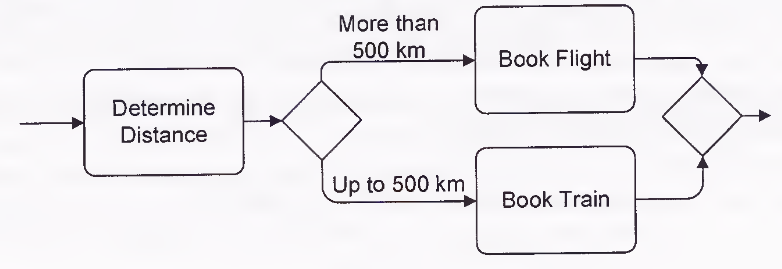
\includegraphics[width=11cm]{./imagenes/gateway_exclusivo.png}
    \caption{Ejemplo de uso del enlace exclusivo}
    \label{fig:gateway_exclusivo}
    \textbf{Fuente:}  \cite{bpmn2}
  \end{center}
\end{figure}

En este caso (Figura \ref{fig:gateway_exclusivo}), se realiza la actividad \textit{Determinar distancia} y se decide que tipo de medio de transporte se debe utilizar. Nótese que luego de realizar la reserva, se vuelve a unir el flujo de secuencia del modelo, ya que no se sabe en la práctica cual de las 2 alternativas será la seleccionada.

\begin{figure}[!htb]
  \begin{center}
    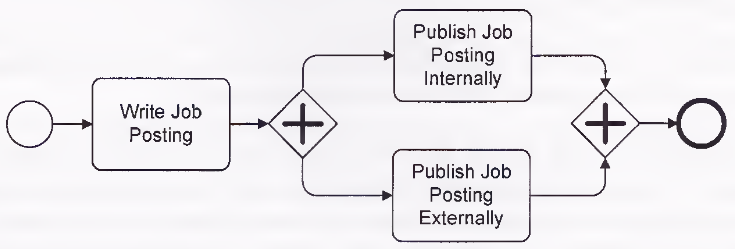
\includegraphics[width=11cm]{./imagenes/gateway_paralelo.png}
    \caption{Ejemplo de uso del enlace paralelo}
    \label{fig:gateway_paralelo}
    \textbf{Fuente:}  \cite{bpmn2}
  \end{center}
\end{figure}

En la figura \ref{fig:gateway_paralelo} se ve un ejemplo de uso de este enlace. Aquí, luego de que se redacta la oferta de trabajo, le procede a publicarla, tanto interna como externamente. En este caso, se utiliza el enlace paralelo para agilizar el proceso de publicación.

\begin{figure}[!htb]
  \begin{center}
    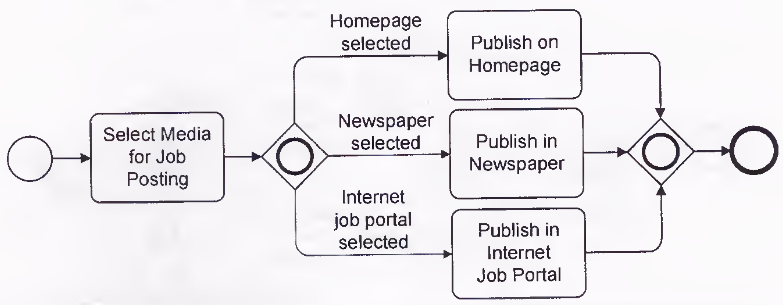
\includegraphics[width=11cm]{./imagenes/gateway_inclusivo.png}
    \caption{Ejemplo de uso del enlace inclusivo}
    \label{fig:gateway_inclusivo}
    \textbf{Fuente:}  \cite{bpmn2}
  \end{center}
\end{figure}


En la figura \ref{fig:gateway_inclusivo} se ve un ejemplo de uso en donde a partir de la actividad ``Seleccionar medio para publicar oferta de trabajo'' se pueden seleccionar una o varias opciones. Cualquier combinación de opciones, que al menos contenga una opción, es válida.

\begin{figure}[!htb]
  \begin{center}
    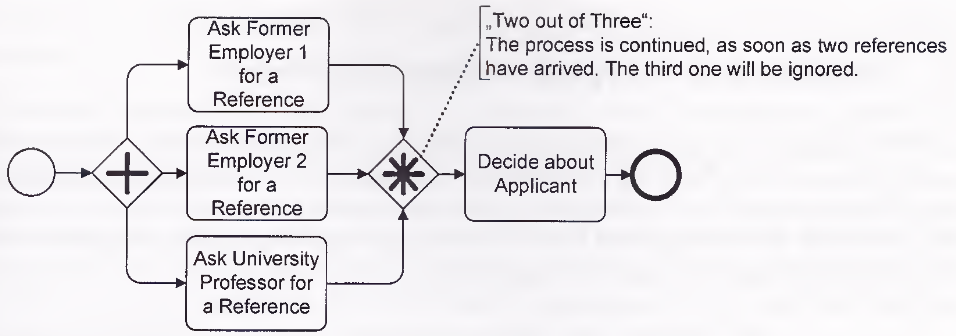
\includegraphics[width=11cm]{./imagenes/gateway_complejo.png}
    \caption{Ejemplo de uso del enlace complejo}
    \label{fig:gateway_complejo}
    \textbf{Fuente:}  \cite{bpmn2}
  \end{center}
\end{figure}


En el ejemplo mostrado en la figura \ref{fig:gateway_complejo}, se requiere la referencia de 2 empleadores previos y de la universidad. En realidad, solo son necesarias dos referencias, pero para estar seguros se piden tres, por lo que tan pronto como llegan las primeras 2 referencias, la tercera puede ser ignorada sin mayor problema.

\subsection{Colaboración}

A menudo, en un proceso intervienen diferentes partes interesadas ({\textit{Stakeholders}) y es necesario ver el proceso de manera global, de manera que el paso de mensajes entre las partes implicadas sea mas claro. A este tipo de diagramas se les llama \textbf{diagrama de colaboración}

La figura \ref{fig:diagrama_colaboracion} muestra como es la interacción entre un aspirante y una empresa en el proceso de acceder a una oferta de empleo. Puede verse como, entre las actividades que ejecuta cada una de las partes, existe un paso de mensaje que une ambos procesos. Esta unión se representa por una flecha con linea punteada, donde un extremo tiene un circulo y el otro una flecha vacía que indica la dirección del mensaje.

\begin{figure}[!htb]
  \begin{center}
    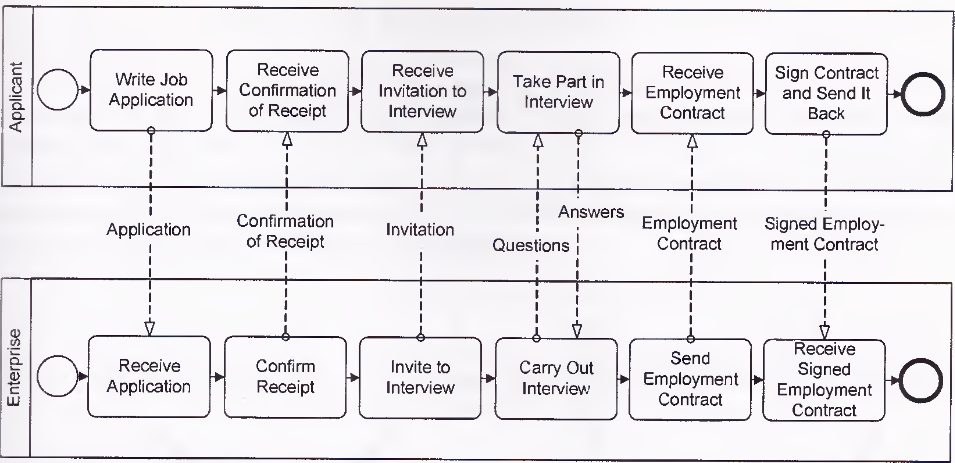
\includegraphics[width=11cm]{./imagenes/diagrama_colaboracion.png}
    \caption{Ejemplo de diagrama de colaboración}
    \label{fig:diagrama_colaboracion}
    \textbf{Fuente:}  \cite{bpmn2}
  \end{center}
\end{figure}


Por ejemplo, la actividad ``Recibir solicitud'' recibe un mensaje de la actividad ``Redactar solicitud de empleo'', por lo cual esta actividad (recibir solicitud) no puede iniciar si el aspirante no envía su solicitud. Esto significa que los mensajes deben ser respetados y una actividad no puede realizarse si le falta algún mensaje de entrada.

Sin embargo, en estos casos solo se conoce el proceso que sigue la empresa, por lo que es común representar a las partes externas como una caja negra (figura \ref{fig:diagrama_colaboracion_caja_negra}).

\begin{figure}[!htb]
  \begin{center}
    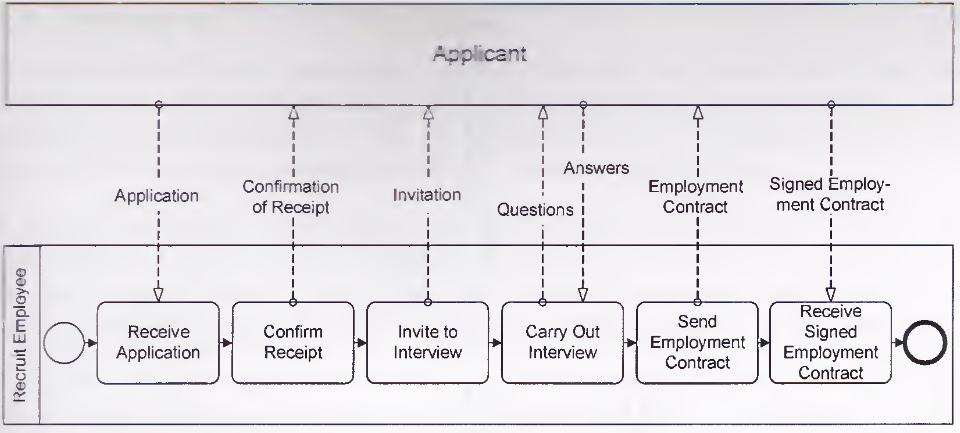
\includegraphics[width=11cm]{./imagenes/diagrama_colaboracion_caja_negra.png}
    \caption{Ejemplo de diagrama de colaboración con caja negra}
    \label{fig:diagrama_colaboracion_caja_negra}
    \textbf{Fuente:}  \cite{bpmn2}
  \end{center}
\end{figure}


\section{SOA}
\subsection{Primeros conceptos}

Los conceptos base del diseño de software deben ser expuestos para tener una mayor claridad en los temas siguientes. A continuación se expresan los conceptos base:

\begin{itemize}
  \item Características de diseño: Son aquellos atributos que cumple un diseño y que pueden ser medidos

  \item Principio de diseño: Es una guía o regla para solucionar un problema de acuerdo a las prácticas aceptadas por la comunidad de ingeniería de software.

  \item Paradigma de diseño: Es el compendio de principios de diseño que tienen un enfoque global común.

  \item Patrones de diseño: Son formas de resolver un problema de diseño que es repetitivo. Viene dado por 3 restricciones presentadas en el diseño de software:
  \begin{itemize}
    \item Restricciones impuestas por la tecnología existente
	  \item Restricciones impuestas por las tecnologías usadas por sistemas transversales
	  \item Restricciones de prioridades de proyectos
  \end{itemize}
  El patrón de diseño describe el problema y da la solución a modo de plantilla.

  \item Lenguajes de patrones de diseño: Es la configuración ordenada de patrones en un diseño lógico. La comunicación entre cada patrón se hace a través de dicho lenguaje.

  \item Estandares de diseño: En orden de ir acorde a las metas, prioridades, recursos y ambiente de la organización en la que se haga el diseño lógico de la solución, un estandar de diseño define convenciones para cada elemento utilizado en el diseño de acuerdo a las características de diseño definidas.

  \item Buenas prácticas: Es una técnica o acercamiento para resolver o prevenir problemas presentados en el desarrollo del diseño lógico de la solución de software. pg 34
\end{itemize}

La figura \ref{fig:uno} presenta un acercamiento a cómo se desarrollan los principios de diseño con los demás conceptos nombrados.

\begin{figure}[!htb]
  \begin{center}
    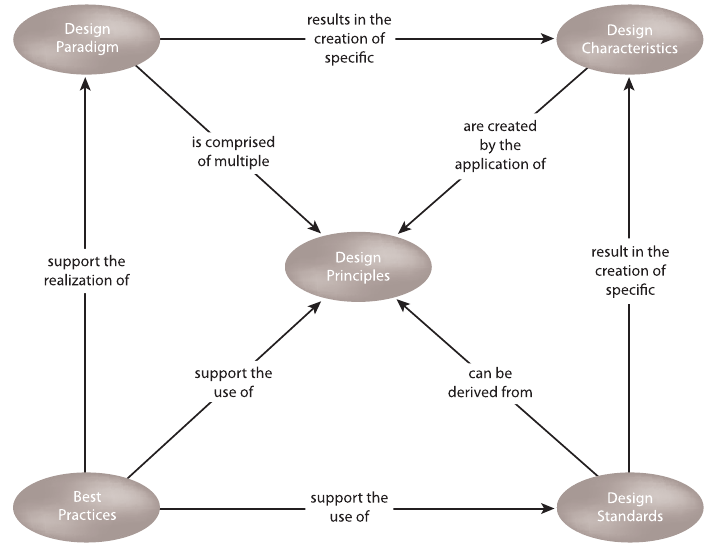
\includegraphics[width=11cm]{./imagenes/1.png}
    \caption{Ejemplo de uso del enlace exclusivo}
    \label{fig:uno}
  \end{center}
\end{figure}

La figura \ref{fig:dos} presenta cómo extiende o soporta un patrón de diseño el diseño lógico de la solución de software.

\begin{figure}[!htb]
  \begin{center}
    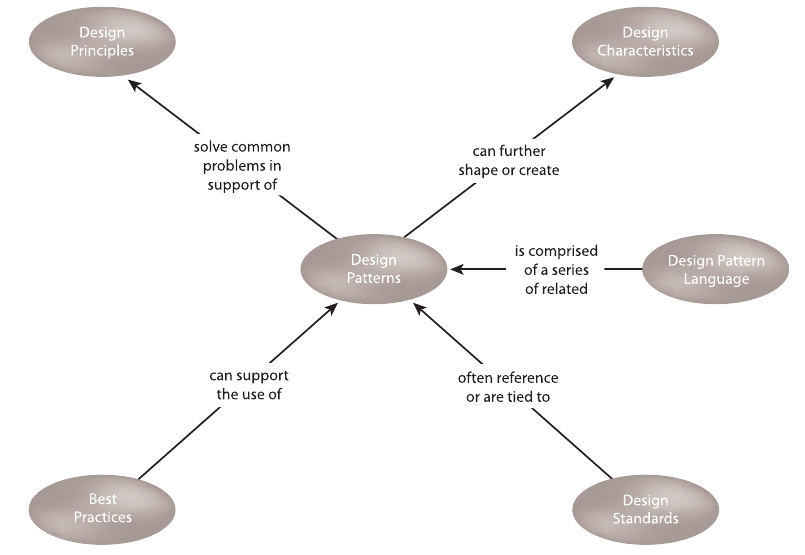
\includegraphics[width=11cm]{./imagenes/2.png}
    \caption{Ejemplo de uso del enlace exclusivo}
    \label{fig:dos}
  \end{center}
\end{figure}

La figura \ref{fig:tres} presenta los componentes que hacen que el diseño lógico de la solución sea acorde al paradigma escogido.

\begin{figure}[!htb]
  \begin{center}
    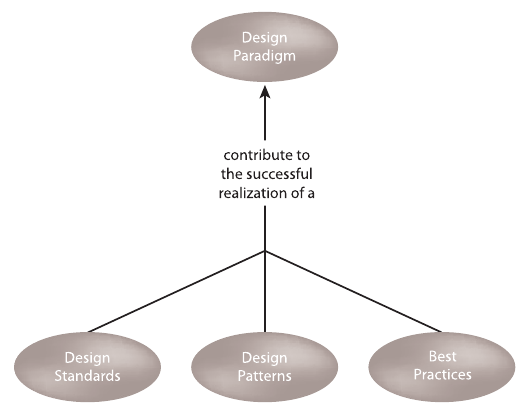
\includegraphics[width=11cm]{./imagenes/3.png}
    \caption{Ejemplo de uso del enlace exclusivo}
    \label{fig:tres}
  \end{center}
\end{figure}

\subsection{Computación orientada a servicios}

La computación orientada a servicios nace de la necesidad de desarrollar software sobre tecnologías distribuidas. Este tipo de computación tiene como finalidad la construcción de inventarios de servicios. La computación orientada a servicios está compuesta por la interacción de la orientación a servicios y la arquitectura orientada a servicios, formando patrones de diseño propios y estándares en cumplimiento de las características de diseño propias de la computación distribuida. Algunos de los conceptos clave llevados en la computación orientada a servicios son:

\begin{itemize}
  \item Arquitectura Orientada a Servicios (SOA - Service Oriented Architecture): Comprende el compendio de tecnologías, APIs, infraestructura y repositorios enmarcados en
el paradigma orientado a servicios y cuyo objetivo principal es el de trabajar sobre el "servicio" como el elemento más importante.

  \item Orientación a servicios: Es el paradigma manejado en la computación orientada a servicios en donde se acepta como unidad mínima y más importante el "servicio"

  \item Servicio: Es un software independiente físicamente el cual tiene asignado un contexto de funcionalidades y que puede ser utilizado por otros servicios por medio
del contrato del servicio (descripción del servicio en cuanto a funcionalidades, entradas requeridas y salidas). De acuerdo a su nivel de reuso, los servicios se dividen en 3 tipos y son:
  \item Servicios entidad: Modela los servicios que se deben ofrecer respecto de las entidades del negocio (ej. empleados y clientes). Tienen un nivel de reuso alto y están centrados en el negocio.
  \item Servicios tarea: Modela los servicios que deben cumplir tareas específicas del negocio (ej. generación de cortes de final de año). Tienen un nivel de reuso bajo. Estos servicios trabajan directamente con 1 o varios servicios entidad. Estos servicios están centrados en el negocio.
  \item Servicios utilidad: Modela servicios que no están centrados en el negocio. Son los servicios con mayor reuso.
La diferenciación entre tipos de servicio da lugar a la estructura en capas mostrada en la figura \ref{fig:cinco}

  \item Composición de servicios: Es la agregación de servicios de manera ordenada.

  \item Inventario de servicios: Es la agrupación de varios servicios según un criterio definido por la organización. Cada inventario de servicios tiene su propio estándar
de diseño e, inclusive, su propia configuración arquitectónica. El desarrollo de los inventarios de servicio es hecho a modo top-down, con la construcción de blueprints (planos).
\end{itemize}

\begin{figure}[!htb]
  \begin{center}
    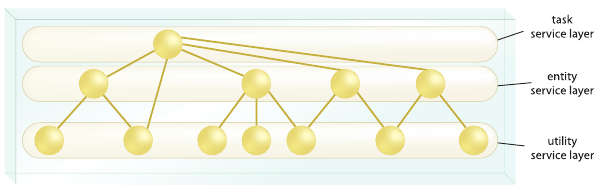
\includegraphics[width=11cm]{./imagenes/5.png}
    \caption{Ejemplo de uso del enlace exclusivo}
    \label{fig:cinco}
  \end{center}
\end{figure}

En la figura \ref{fig:cuatro} se muestra la interacción de los conceptos clave en la computación orientada a servicios.

\begin{figure}[!htb]
  \begin{center}
    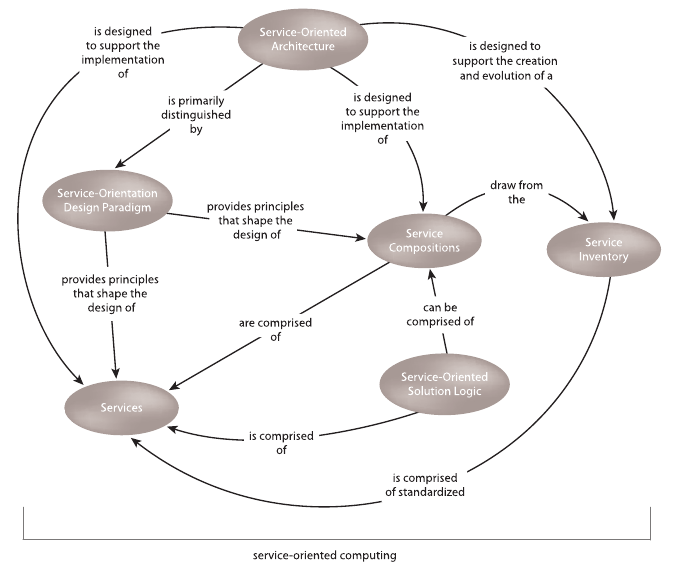
\includegraphics[width=11cm]{./imagenes/4.png}
    \caption{Ejemplo de uso del enlace exclusivo}
    \label{fig:cuatro}
  \end{center}
\end{figure}


\section{Scrum}

A continuación, se explican los diferentes roles y artefactos que existen en el marco de trabajo de Scrum.

\subsection{Equipo Scrum (Scrum Team)}

\subsubsection{Product Owner (dueño del producto)}

Es el responsable de gestionar el product backlog y el trabajo del equipo de desarrollo. Entre sus funciones se encuentran:
\begin{itemize}
		  \item Expresar los elementos del product backlog.
		  \item Ordenar de la mejor manera posible los elementos del product backlog para lograr el objetivo final.
		  \item Asegurarse de que el equipo de desarrollo entiende los items del product backlog.
		\end{itemize}
		
\subsubsection{Development Team (Equipo de desarrollo)}

Son los encargados de llevar a cabo el incremento al producto en cada iteración o sprint. El equipo de desarrollo es el encargado de organizar y gestionar su propio trabajo.

El equipo de desarrollo se caracteriza por:
	
\begin{itemize}
		  \item Es autoorganizado: Se le dice al equipo que debe hacer, pero el es libre de decidir como lo hace.
		  \item Son multifuncionales: Se tienen integrantes que manejan diferentes áreas de experticia para ayudar a realizar el incremento necesario.
		  \item No se reconocen los sub-equipos que se puedan formar, la responsabilidad de lo que se haga recae en e equipo de desarrollo como un todo.
		\end{itemize}

\subsubsection{Scrum Master}

Es el encargado de que se cumpla la teoría de scrum a lo largo de todo el proyecto. El Scrum Master ayuda a las personas externas al Equipo Scrum a entender qué interacciones con el Equipo Scrum pueden ser de ayuda y cuáles no \cite{scrum_guide}.

\textbf{Servicios que ofrece al Product Owner}
	
\begin{itemize}
		  \item Encontrar técnicas para gestionar la Lista de Producto de manera efectiva
		  \item Ayudar al Equipo Scrum a entender la necesidad de contar con elementos de Lista de Producto claros y concisos
		  \item Entender la planificación del producto en un entorno empírico
		  \item Asegurar que el Dueño de Producto conozca cómo ordenar la Lista de Producto para maximizar el valor
		  \item Entender y practicar la agilidad; y,
		  \item Facilitar los eventos de Scrum según se requiera o necesite.
\end{itemize}
		\cite{scrum_guide}

\textbf{Servicios que ofrece al Developement Team}
	
\begin{itemize}
		  \item Guiar al Equipo de Desarrollo en ser autoorganizado y multifuncional;
		  \item Ayudar al Equipo de Desarrollo a crear productos de alto valor;
		  \item Eliminar impedimentos para el progreso del Equipo de Desarrollo;
		  \item Facilitar los eventos de Scrum según se requiera o necesite; y,
		  \item Guiar al Equipo de Desarrollo en el entorno de organizaciones en las que Scrum aún no ha sido adoptado y entendido por completo.
\end{itemize}
		\cite{scrum_guide}

\textbf{Servicios que ofrece a la organización}
	
\begin{itemize}
		  \item Liderar y guiar a la organización en la adopción de Scrum;
		  \item Planificar las implementaciones de Scrum en la organización; 
		  \item Ayudar a los empleados e interesados a entender y llevar a cabo Scrum y el desarrollo empírico de producto;
		  \item Motivar cambios que incrementen la productividad del Equipo Scrum; y,
		  \item Trabajar con otros Scrum Masters para incrementar la efectividad de la aplicación de Scrum en la organización.
\end{itemize}
		\cite{scrum_guide}
		
\subsection{Eventos}

\subsubsection{Sprint}

El Sprint representa un espacio de tiempo, no mayor a un mes, en el que se trabaja para crear un incremento en el desarrollo del proyecto. Es conveniente que los sprint tengan una duración consistente a lo largo del proyecto, y un nuevo sprint inicia tan pronto el actual termina.

Cada sprint debe tener un objetivo definido (Sprint Goal), un plan flexible y concepto de ``terminado'' claro. 

\subsubsection{Sprint Planning Meeting (Reunión de Planificación de Sprint)}

Esta reunion se lleva a cabo al inicio de cada Sprint y no tiene una duración mayor a 8 horas. En esta reunión, que se lleva a cabo en presencia de todo el equipo scrum, se crea un plan para el sprint que inicia. En este plan se responden dos preguntas fundamentales, ¿Qué puede entregarse en el Incremento resultante del Sprint que comienza? y ¿Cómo se conseguirá hacer el trabajo necesario para entregar el Incremento?

\subsubsection{Daily Scrum (Scrum Diario)}

Esta reunion, que no debe durar mas de 15 minutos, se realiza a diario entre los miembros del development team. El objetivo de esta reunion es socializar lo que se hizo en las ultimas 24 horas y planear que hacer en las proximas 24 horas. Se evalua si se esta haciendo lo necesario para cumplir el sprint goal y, si es necesario, se puede adaptar o redefinir el trabajo del resto del sprint.

\subsubsection{Sprint Review (Revisión de Sprint)}

Al final de cada sprint se realiza esta reunion cuyo objetivo es el de socializar lo que se hizo en el presente sprint. En esta reunion se descuten cosas como qué fue bien durante el Sprint, qué problemas aparecieron y cómo fueron resueltos esos problemas. Al final de la revisión se debe generar un product backlog actualizado con los elementos que se proponen para el siguiente sprint. Esta reunion tiene una duracion no mayor a 4 horas.

\subsubsection{Sprint Retrospective (Retrospectiva de Sprint)}

Esta reunión es similar al sprint review, pero en lugar de tratar el Qué se hizo, se trata el Cómo se hizo. Al final de esta reunión se genera un plan para mejorar el desempeño del equipo de scrum para que los sprint posteriores sean de mayor provecho para el proyecto.

\subsection{Artefactos}

\subsubsection{Sprint Goal (Objetivo del Sprint)}

El sprint goal es una meta que se plantea al inicio de cada sprint que puede ser alcanzada mediante el incremento en el proyecto. Este sprint goal ``Proporciona una guía al Equipo de Desarrollo acerca de por qué está construyendo el incremento'' \cite{scrum_guide}. Es importante y necesario que el objetivo sea claro, coherente y sea entendido por todos los integrantes del equipo de scrum.

\subsubsection{Product Backlog (Lista de Producto)}

Esta lista representa todos los requisitos que tenga el proyecto o producto que son conocidos y entendidos en un momento determinado del desarrollo. Debido a la naturaleza cambiante y dinámica del entorno, la lista nunca está vacía. A medida que el producto evoluciona, la retroalimentación que se obtiene ayuda a completar la lista y a refinar el producto final.

\subsubsection{Sprint Backlog (Lista de Pendientes del Sprint)}

Esta lista esta compuesta por los diferentes items seleccionados del broduct backlog que van a ser tratados en cada sprint. Adicionalmente, se incluye un plan que ayude a conseguir el objetivo del sprint.
	
La Lista de Pendientes del Sprint es una predicción hecha por el Equipo de Desarrollo acerca de qué funcionalidad formará parte del próximo Incremento y del trabajo necesario para entregar esa funcionalidad en un Incremento \cite{scrum_guide}.


Una vez habiendo puesto en contexto el problema a resolver en los anteriores capítulos (en especial el capítulo \ref{chap:definicion_problema}), en este capítulo se encuentra una descripción un poco más concisa de los requerimientos funcionales encontrados por los autores y, también, los requerimientos no funcionales que serán tomados en cuenta a la hora de evaluar la calidad del prototipo del SNS desarrollado.

\section{Requerimientos funcionales}
La identificación de los requerimientos funcionales consignados en éste capítulo fue la base para realizar la arquitectura del software a implementar.

Se identificaron, en el análisis de requerimientos, 14 posibles módulos enunciados a continuación:

\begin{enumerate}
	\item \textbf{Gestión de usuarios*}: Módulo que controla características inherentes a todos los tipos de usuario de la red social en cuanto al manejo de su información personal y roles que cumplen
	\item \textbf{Gestión de deportes*}: Módulo por medio del cual se controla la información detallada de un deporte
	\item \textbf{Gestión de equipos}: Módulo que ayuda a la gestión de datos competentes a equipos deportivos
	\item \textbf{Gestión de torneos}: Módulo que suple las necesidades de un organizador de eventos cuando éste desea trabajar con la información de un torneo deportivo
	\item \textbf{Gestión de eventos deportivos*}: Módulo que brinda funcionalidades de gestión de eventos deportivos
	\item \textbf{Gestión de patrocinadores}: Módulo que brinda funcionalidades al patrocinador que lo use, para patrocinar y controlar patrocinios, así como para seguir actividad de posibles patrocinados.
	\item \textbf{Gestión de organizaciones}: Módulo que ofrece funciones de gestión de organizaciones
	\item \textbf{Gestión de self-expression}: Módulo que es utilizado para el manejo de contenido propio generado por un actor en la red social o un evento que uno o más actores manejen en la red social
	\item \textbf{Gestión del conocimiento}: Módulo que gestiona artículos/post relacionados con tips en campos de salud y deportivos en si
	\item \textbf{Gestión de geolocalización*}: Módulo que ayuda al control de todas las funcionalidades de geolocalización
	\item \textbf{Gestión de estadísticas}: Módulo que permite la generación y visualización de estadísticas diversas acerca de deportistas, organizaciones, ubicaciones o cualquier otro concepto que maneje estadísticas en el SNS
	\item \textbf{Gestión de entrenadores}: Módulo que permite la gestión de opcionalidades ofrecidas a entrenadores deportivos, tal como el seguimiento de entrenados o la asignación de planes deportivos a los mismos
	\item \textbf{Gestión de canales de difusión}: Módulo que refiere a todo lo relacionado con noticias deportivas
	\item \textbf{Gestión de grupos deportivos}:  Módulo de gestión de funcionalidades ofrecidas a grupos deportivos informales (diferentes a los equipos deportivos, caso especial de los grupos deportivos)
\end{enumerate}

Para el desarrollo del prototipo, los autores se concentran en los módulos marcados con * en la anterior lista. Para saber los criterios por los cuales se han escogido éstos módulos, el lector puede dirigirse a \ref{chap:alcances_limitaciones}.

La lista de requerimientos puede encontrarse en \ref{app:req_funcionales}.

\section{Requerimientos no funcionales}
Los requerimientos no funcionales explorados en detalle para el desarrollo del SNS deportivo y que son tenidos en cuenta se presentan a continuación con escenarios de calidad (reducidos; los escenarios completos se encuentran en \cite{anexos_tesis}), los cuales son descritos como los escenarios en los que se probará la calidad del software desarrollado.

\subsubsection{QiU}

En esta sección se da una versión simplificada del análisis de escenarios de calidad correspondientes a las áreas de usabilidad y UX.

\begin{itemize}
	\item \textbf{Escenario de calidad 1}: Busca que el usuario pueda realizar todas las tareas que desea realizar con el SNS
	\item \textbf{Escenario de calidad 2}: Busca que las funcionalidades ofrecidas por el SNS se ejecuten en un tiempo corto
	\item \textbf{Escenario de calidad 3}: Busca que el nivel de conformidad con la interfaz de usuario (UX) sea marcado
	\item \textbf{Escenario de calidad 4}: Busca que el usuario aprenda a utilizar las principales funcionalidades del SNS en poco tiempo
	\item \textbf{Escenario de calidad 5}: Busca hacer legible cada mensaje de error que aparezca cada vez que se produzca uno en el SNS
	\item \textbf{Escenario de calidad 6}: Busca hacer conciente al usuario de los diferentes roles manejados a través de la red social
	\item \textbf{Escenario de calidad 7}: Busca que el usuario conozca todas las funcionalidades ofrecidas por el SNS
	\item \textbf{Escenario de calidad 8}: Busca que el usuario sea efectivo a la hora de utilizar cada funcionalidad
\end{itemize}

\subsubsection{Reusabilidad}

Para el desarrollo de escenarios de calidad en cuanto a reusabilidad se refiere, se utilizaron apartes de \cite{soa_principles} para definirlos. A continuación se exponen los escenarios de calidad resumidos.

\begin{itemize}
	\item \textbf{Escenario de calidad 1}: Busca que el software cumpla con la reusabilidad táctica
	\item \textbf{Escenario de calidad 2}: Busca dar a los servicios hechos en la red social, en su mayoría, un carácter agnóstico
	\item \textbf{Escenario de calidad 3}: Busca la estandarización del nombramiento de las diferentes partes de los contratos de servicio a crear
\end{itemize}

\subsubsection{Mantenibilidad}

A continuación se exponen escenarios de calidad resumidos relacionados a la mantenibilidad, tomando como base tanto el paradigma orientado a servicios como elementos del estandar ISO/IEC 9126.

\begin{itemize}
	\item \textbf{Escenario de calidad 1}: Busca mayor adaptación del software a capacidades nuevas
	\item \textbf{Escenario de calidad 2}: Busca disminuir la cantidad de lógica envuelta por un servicio
	\item \textbf{Escenario de calidad 3}: Busca que los servicios tengan una complejidad tan manejable como sea posible
\end{itemize}

\subsubsection{Interoperabilidad}

En \cite{soa_principles}, se hace referencia a la interoperabilidad como un componente transversal a todo principio, patrón y demás concepto manejado en el paradigma orientado a servicios. A continuación se describe el escenario de calidad resumido estipulado por los autores.

\begin{itemize}
	\item \textbf{Escenario de calidad 1}: Busca la adopción de una política estricta de estandarización al momento del desarrollo de los contratos de servicio
\end{itemize}

\subsubsection{Seguridad}

Se tuvieron en cuenta los principios de seguridad expresados en \cite{security_ws}. A continuación se enuncian los escenarios de calidad resumidos estipulados por el lado de la seguridad.

\begin{itemize}
	\item \textbf{Escenario de calidad 1}: Busca aplicar el concepto de ''Fail Securely''
	\item \textbf{Escenario de calidad 2}: Busca deshabilitar toda funcionalidad no terminada y accesos a ellas
	\item \textbf{Escenario de calidad 3}: Busca establecer un sistema de autenticación-autorización
	\item \textbf{Escenario de calidad 4}: Busca la encripción de mensajes pasados entre servicios
\end{itemize}

\subsubsection{Rendimiento}

Para el rendimiento, \cite{time_response}, se tuvo en cuenta una sola medida: Las funcionalidades que no dependan de la carga o descarga de una cantidad de información grande (ej. videos e imágenes) no deberán tardar más de 5 segundos.

\section{Archimate 2.0}

Según  \cite{archimate2}, archimate es un lenguaje estandar utilizado por los arquitectos de software para modelar las necesidades de cada \textit{stakeholder}, dividiendo el contexto en el que se desenvuelve el software a desarrollar en tres capas: capa de negocio, capa de aplicación y capa de tecnología.

\subsection{Capas de archimate}

A continuación serán descritas las tres capas definidas en el estandar archimate.

\subsubsection{Capa de negocio}

Esta capa envuelve todos los conceptos relacionados con la organización sobre la cual se aplicará el software a desarrollar, esto es, los roles, los servicios ofrecidos, los procesos, los productos y demás conceptos aplicados sobre su estructura y dinámica. Los artefactos de esta capa utilizados en el proyecto se enuncian en el cuadro \ref{tab:artefactos_capa_negocio}.

 \begin{center}
 
 	\textbf{Fuente:} \cite{archimate2}
 	
	\begin{longtable}{|p{4cm}|p{6cm}|c|}
	\caption{Artefactos de la capa de negocio \label{tab:artefactos_capa_negocio}} \\
	\hline
    \textbf{Artefacto} & 
    \textbf{Descripción} & 
    \textbf{Notación} \\ 
    \hline
	\endfirsthead
    \hline
    \textbf{Artefacto} & 
    \textbf{Descripción} & 
    \textbf{Notación} \\ 
    \hline
	\endhead
    \hline
	\endfoot
	\hline
	\endlastfoot
    \hline
    \textit{Actor de negocio (Business actor)} & 
    Ente (persona) organizacional quien cumple tareas en la organización &  
    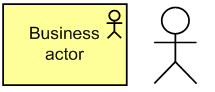
\includegraphics[width=1.5cm]{./imagenes/Archimate/businessactor.png}\\
	\hline
	\textit{Colaboración de negocio (Business collaboration)} & 
    Rol que surge de la combinación de dos o más roles &  
    \includegraphics[width=1.5cm]{./imagenes/Archimate/businesscollaboration.png}\\
	\hline    
    \textit{Rol de negocio (Business role)} & 
    Es un conjunto de responsabilidades que tiene asignado un actor. Dicho conjunto está definido por un solo concepto (nombre) &  
    \includegraphics[width=1.5cm]{./imagenes/Archimate/businessrole.png}\\
    \hline
    \textit{Proceso de negocio (Business process)} & 
    Agrupa comportamientos que se ejecutan como una serie de pasos &  
    \includegraphics[width=1.5cm]{./imagenes/Archimate/businessprocess.png}\\
	\hline
	\textit{Función de negocio (Business function)} & 
    Agrupa comportamientos que requieren una serie de competencias o recursos de negocio &  
    \includegraphics[width=1.5cm]{./imagenes/Archimate/businessfunction.png}\\
	\hline
	\textit{Interacción de negocio (Business interaction)} & 
    Comportamientos realizados por colaboraciones de negocio &  
    \includegraphics[width=1.5cm]{./imagenes/Archimate/businessinteraction.png}\\
	\hline
	\textit{Evento de negocio (Business event)} & 
    Hecho que dispara un comportamiento (o grupo de comportamientos) en la organización &  
    \includegraphics[width=1.5cm]{./imagenes/Archimate/businessevent.png}\\
	\hline
	\textit{Servicio de negocio (Business service)} & 
    Servicio que cumple una necesidad del usuario &  
    \includegraphics[width=1.5cm]{./imagenes/Archimate/businessservice.png}\\
	\hline
	\textit{Producto (Product)} & 
    Agrupación de servicios que, definidos por un contrato, serán compartidos a clientes (tanto roles dentro de la organización como para clientes externos) &  
    \includegraphics[width=1.5cm]{./imagenes/Archimate/businessproduct.png}\\
	\hline
  \end{longtable}
\end{center}

\subsubsection{Capa de aplicación} 

Esta capa cubre los conceptos relacionados con el modelamiento del sistema de información que soporta el negocio (la organización), previamente modelado en la capa de negocio. Los artefactos de esta capa utilizados en el proyecto se enuncian en el cuadro \ref{tab:artefactos_capa_aplicacion}.

\begin{table}
  \caption{Artefactos de la capa de aplicación}
  \label{tab:artefactos_capa_aplicacion}

  \begin{center}
  
  \textbf{Fuente:} \cite{archimate2}
  
  \resizebox{15cm}{!}{
  \begin{tabular}{|L{3cm}|L{6cm}|c|}
    \hline
    \textbf{Artefacto} & \textbf{Descripción} & \textbf{Notación} \\ 
    \hline
    \textit{Componente de aplicación (Application component)} & 
    Unidad de software &  
    \includegraphics[width=1.5cm]{./imagenes/Archimate/applicationcomponent.png}\\
	\hline
	\textit{Colaboración de aplicación (Application collaboration)} & 
    Colaboración entre dos o más componentes de aplicación para realizar una tarea que necesita de cada uno de ellos &  
    \includegraphics[width=1.5cm]{./imagenes/Archimate/applicationcollaboration.png}\\
	\hline    
    \textit{Función de aplicación (Application function)} & 
    Agrupa comportamientos que pueden ser automatizados por un componente de aplicación &  
    \includegraphics[width=1.5cm]{./imagenes/Archimate/applicationfunction.png}\\
    \hline
    \textit{Interacción de aplicación (Application interaction)} & 
    Agrupa comportamientos que pueden ser automatizados por una colaboración de aplicación &  
    \includegraphics[width=1.5cm]{./imagenes/Archimate/applicationinteraction.png}\\
	\hline
	\textit{Servicio de aplicación (Application service)} & 
    Un servicio que expone las funcionalidades automatizadas ofrecidas &  
    \includegraphics[width=1.5cm]{./imagenes/Archimate/applicationservice.png}\\
	\hline
  \end{tabular}
  }
    \end{center}
\end{table}

\subsubsection{Capa de tecnología}

Capa que modela el posicionamiento físico del software a utilizar, así como también los requerimientos que este tiene para su funcionamiento a nivel físico (servidores, redes, nodos, etc.). Los artefactos de esta capa utilizados en el proyecto se enuncian en el cuadro \ref{tab:artefactos_capa_tecnologia}.


\begin{table}
  \caption{Artefactos de la capa de tecnología}
  \label{tab:artefactos_capa_tecnologia}

  \begin{center}
  
  \textbf{Fuente:} \cite{archimate2}
  
  \resizebox{15cm}{!}{
  \begin{tabular}{|L{3cm}|L{6cm}|c|}
    \hline
    \textbf{Artefacto} & \textbf{Descripción} & \textbf{Notación} \\ 
    \hline
    \textit{Nodo (Node)} & 
    Recurso computacional que agrupa artefactos almacenables o desplegables para ser ejecutados &  
    \includegraphics[width=1.5cm]{./imagenes/Archimate/technologynode.png}\\
	\hline
	\textit{Dispositivo (Device)} & 
    Hardware que contiene elementos software para ser ejecutados &  
    \includegraphics[width=1.5cm]{./imagenes/Archimate/technologydevice.png}\\
	\hline    
    \textit{Red (Network)} & 
    Medio de comunicación entre dos o más nodos o dispositivos &  
    \includegraphics[width=1.5cm]{./imagenes/Archimate/technologynetwork.png}\\
    \hline
    \textit{Sistema de software (System software)} & 
    Software sobre el cual se realizan (o representan) los artefactos (componentes de aplicación) desplegables &  
    \includegraphics[width=1.5cm]{./imagenes/Archimate/technologyswsystem.png}\\
	\hline
	\textit{Servicio de infraestructura (Infraestructure service)} & 
    Servicios que agrupan funcionalidades prestadas por nodos &  
    \includegraphics[width=1.5cm]{./imagenes/Archimate/technologyservice.png}\\
	\hline
  \end{tabular}
  }
    \end{center}
\end{table}

\subsection{Relaciones}

Las relaciones, en archimate, son aquellas conexiones existentes entre dos artefactos. Hay tres tipos de relaciones en archimate: relaciones estructurales, relaciones dinámicas y otras que no caben en las dos últimas.

\begin{itemize}

\item \textbf{Relaciones estructurales}: Estas relaciones modelan la coherencia estructural generada por la unión estructural de todos los artefactos de la arquitectura. En el cuadro \ref{tab:relaciones_estructurales} se hace un sumario de las relaciones estructurales utilizadas para unir los artefactos utilizados en el presente proyecto:

\begin{table}
  \caption{Relaciones estructurales}
  \label{tab:relaciones_estructurales}

  \begin{center}
  
  \textbf{Fuente:} \cite{archimate2}
  
  \resizebox{15cm}{!}{
  \begin{tabular}{|L{3cm}|L{7cm}|c|}
    \hline
    \textbf{Relación} & \textbf{Descripción} & \textbf{Notación} \\ 
    \hline
    \textit{Asociación (Association)} & 
    Cumple la función de asociar dos artefactos que no tienen una relación más específica &  
    \includegraphics[width=1cm]{./imagenes/Archimate/relassociation.png}\\
	\hline
	\textit{Usado por (Used by)} & 
    Modela el acceso a servicios o interfaces. El acceso a interfaces solo puede ser realizado por artefactos estructurales y a los servicios solo los artefactos comportamentales &  
    \includegraphics[width=1cm]{./imagenes/Archimate/relusedby.png}\\
	\hline    
    \textit{Realización (Realization)} & 
    Une un artefacto abstracto con otro más concreto que lo realiza &  
    \includegraphics[width=1cm]{./imagenes/Archimate/relrealization.png}\\
    \hline
    \textit{Asignación (Assignment)} & 
    Une artefactos con aquellos que, por obligación, deben utilizar otros (por ejemplo, un rol con una función de negocio) &  
    \includegraphics[width=1cm]{./imagenes/Archimate/relassignment.png}\\
	\hline
	\textit{Agregación (Aggregation)} & 
    Es la composición de un artefacto por otros. Esta composición no es destructiva, es decir, si el artefacto que es compuesto deja de existir, los otros seguirán existiendo &  
    \includegraphics[width=1cm]{./imagenes/Archimate/relaggregation.png}\\
	\hline
	\textit{Composición (Composition)} & 
    Es la composición de un artefacto por otros. Esta composición es destructiva, es decir, si el artefacto que es compuesto deja de existir, los otros también &  
    \includegraphics[width=1cm]{./imagenes/Archimate/relcomposition.png}\\
	\hline
  \end{tabular}
  }
    \end{center}
\end{table}

\item \textbf{Relaciones dinámicas}: Esta relación expresa una unión temporal entre dos artefactos donde, posiblemente, uno de los artefactos use a otro para cumplir un fin específico.En el cuadro \ref{tab:relaciones_dinamicas} se hace un sumario de las relaciones dinámicas utilizadas para unir los artefactos utilizados en el presente proyecto.

\begin{table}
  \caption{Relaciones dinámicas}
  \label{tab:relaciones_dinamicas}

  \begin{center}
  
  \textbf{Fuente:} \cite{archimate2}
  
  \resizebox{15cm}{!}{
  \begin{tabular}{|L{3cm}|L{7cm}|c|}
    \hline
    \textbf{Relación} & \textbf{Descripción} & \textbf{Notación} \\ 
    \hline
    \textit{Flujo (Flow)} & 
    Describe intercambios de información entre artefactos comportamentales &  
    \includegraphics[width=1.5cm]{./imagenes/Archimate/relflow.png} 
    \\
	\hline
	\textit{Disparador (Triggering)} & 
    Describe la relación temporal o factual entre 2 artefactos comportamentales &  
    \includegraphics[width=1.5cm]{./imagenes/Archimate/reltriggering.png}
    \\
	\hline
  \end{tabular}
  }
    \end{center}
\end{table}

\item \textbf{Otras relaciones}: En el cuadro \ref{tab:otras_relaciones} se hace un sumario de las relaciones que no pueden ser incluidas en las dinámicas o en las estructurales y que son utilizadas para unir los artefactos utilizados en el presente proyecto.

\begin{table}
  \caption{Otras relaciones}
  \label{tab:otras_relaciones}

  \begin{center}
  
  \textbf{Fuente:} \cite{archimate2}
  
  \resizebox{15cm}{!}{
  \begin{tabular}{|L{3cm}|L{7cm}|c|}
    \hline
    \textbf{Relación} & \textbf{Descripción} & \textbf{Notación} \\ 
    \hline
    \textit{Unión (Junction)} & 
    Cumple la función de asociar dos artefactos que no tienen una relación más específica &  
    \includegraphics[width=1cm]{./imagenes/Archimate/reljunction.png}\\
	\hline
	\textit{Especialización (Specialization)} & 
    Indica la especialización de un artefacto tomando otro como referencia &  
    \includegraphics[width=1cm]{./imagenes/Archimate/relspecialization.png}\\
	\hline
  \end{tabular}
  }
    \end{center}
\end{table}

\end{itemize}

\subsection{Vistas archimate}

Debido a la existencia de diferentes stakeholders en el desarrollo de software, se hace necesario mostrar aquella parte de la arquitectura que cierto stakeholder necesita para tener una vista entera del negocio, el sistema de información o la infraestructura, o bien una combinación de ellos.

Archimate utiliza el concepto de “vistas” como la segmentación de la arquitectura en vistas que conciernen al stakeholder que quiera echar un vistaso a la arquitectura, escondiendo detalles de la arquitectura que no le interesan a este.

En los cuadros \ref{tab:introductory_viewpoint} a \ref{tab:infrastructure_viewpoint} se pueden ver las vistas utilizadas, con su descripción y su metamodelo.

\begin{table}
  \caption{Punto de vista introductorio}
  \label{tab:introductory_viewpoint}

  \begin{center}
  
  \textbf{Fuente:} \cite{archimate2}
  
  \resizebox{15cm}{!}{
  \begin{tabular}{|L{4cm}|L{11cm}|}
    \hline
    \textbf{Punto de vista} & 
    Punto de vista introductorio (introductory viewpoint) \\ 
    \hline
    \textbf{Stakeholders} & 
    Arquitectos empresariales y gerentes generales \\ 
    \hline
    \textbf{Concerns} & 
    Da un panorama de los cambios, representaciones o adiciones del o a la organización. Ayuda a la toma de decisiones \\ 
    \hline
    \textbf{Propósito} & 
    Diseñar, decidir e informar \\ 
    \hline
    \textbf{Capas} & 
    Negocio, aplicación e infraestructura \\ 
    \hline
    \textbf{Metamodelo} &
    \includegraphics[width=7cm]{./imagenes/Archimate/introductoryviewpoint.png}\\
	\hline
  \end{tabular}
  }
    \end{center}
\end{table}

\begin{table}
  \caption{Punto de vista en capas}
  \label{tab:layered_viewpoint}

  \begin{center}
  
  \textbf{Fuente:} \cite{archimate2}
  
  \resizebox{15cm}{!}{
  \begin{tabular}{|L{4cm}|L{11cm}|}
    \hline
    \textbf{Punto de vista} & 
    Punto de vista en capas (layered viewpoint) \\ 
    \hline
    \textbf{Stakeholders} & 
    Arquitectos de dominio, infraestructura, procesos, aplicación y negocio \\ 
    \hline
    \textbf{Concerns} & 
    Impacto del cambio, flexibilidad, reducción de la complejidad y consistencia \\ 
    \hline
    \textbf{Propósito} & 
    Diseñar, decidir e informar \\ 
    \hline
    \textbf{Capas} & 
    Negocio, aplicación e infraestructura \\ 
    \hline
    \textbf{Metamodelo} &
    Se usan los artefactos y relaciones de todas las capas, según se considere pertinente\\
	\hline
  \end{tabular}
  }
    \end{center}
\end{table}

\begin{table}
  \caption{Punto de vista de función}
  \label{tab:business_function_viewpoint}

  \begin{center}
  
  \textbf{Fuente:} \cite{archimate2}
  
  \resizebox{15cm}{!}{
  \begin{tabular}{|L{4cm}|L{11cm}|}
    \hline
    \textbf{Punto de vista} & 
    Punto de vista de función (business function viewpoint) \\ 
    \hline
    \textbf{Stakeholders} & 
    Organización, arquitectos de proceso y de dominio \\ 
    \hline
    \textbf{Concerns} & 
    Identificación de competencias, identificación de actividades principales y reducción de complejidad \\ 
    \hline
    \textbf{Propósito} & 
    Diseño \\ 
    \hline
    \textbf{Capas} & 
    Negocio \\ 
    \hline
    \textbf{Metamodelo} &
    \includegraphics[width=7cm]{./imagenes/Archimate/businessfunctionviewpoint.png}\\
	\hline
  \end{tabular}
  }
    \end{center}
\end{table}

\begin{table}
  \caption{Punto de vista de proceso}
  \label{tab:business_process_viewpoint}

  \begin{center}
  
  \textbf{Fuente:} \cite{archimate2}
  
  \resizebox{15cm}{!}{
  \begin{tabular}{|L{4cm}|L{11cm}|}
    \hline
    \textbf{Punto de vista} & 
    Punto de vista de proceso (business process viewpoint) \\ 
    \hline
    \textbf{Stakeholders} & 
    Gerentes operacionales, aquitectos de dominio y de proceso \\ 
    \hline
    \textbf{Concerns} & 
    Estructura del proceso de negocio, consistencia y completitud así como también responsabilidades \\ 
    \hline
    \textbf{Propósito} & 
    Diseño \\ 
    \hline
    \textbf{Capas} & 
    Negocio y aplicación \\ 
    \hline
    \textbf{Metamodelo} &
    \includegraphics[width=7cm]{./imagenes/Archimate/businessprocessviewpoint.png}\\
	\hline
  \end{tabular}
  }
    \end{center}
\end{table}

\begin{table}
  \caption{Punto de vista de uso de aplicación}
  \label{tab:application_usage_viewpoint}

  \begin{center}
  
  \textbf{Fuente:} \cite{archimate2}
  
  \resizebox{15cm}{!}{
  \begin{tabular}{|L{4cm}|L{11cm}|}
    \hline
    \textbf{Punto de vista} & 
    Punto de vista de uso de aplicación (Application usage viewpoint) \\ 
    \hline
    \textbf{Stakeholders} & 
    Arquitectos de proceso, arquitectos de negocio, arquitectos de aplicación y gerentes operacionales \\ 
    \hline
    \textbf{Concerns} & 
    Competencia y completitud, reducción de la complejidad \\ 
    \hline
    \textbf{Propósito} & 
    Diseño y decisión \\ 
    \hline
    \textbf{Capas} & 
    Negocio y aplicación \\ 
    \hline
    \textbf{Metamodelo} &
    \includegraphics[width=7cm]{./imagenes/Archimate/applicationusageviewpoint.png}\\
	\hline
  \end{tabular}
  }
    \end{center}
\end{table}

\begin{table}
  \caption{Punto de vista de producto}
  \label{tab:product_viewpoint}

  \begin{center}
  
  \textbf{Fuente:} \cite{archimate2}
  
  \resizebox{15cm}{!}{
  \begin{tabular}{|L{4cm}|L{11cm}|}
    \hline
    \textbf{Punto de vista} & 
    Punto de vista de producto (Product viewpoint) \\ 
    \hline
    \textbf{Stakeholders} & 
    Desarrolladores de producto, gerentes de producto y de proceso, también los arquitectos de dominio \\ 
    \hline
    \textbf{Concerns} & 
    Desarrollo de producto y muestra del valor ofrecido por los productos de la organización \\ 
    \hline
    \textbf{Propósito} & 
    Diseño y decisión \\ 
    \hline
    \textbf{Capas} & 
    Negocio y aplicación \\ 
    \hline
    \textbf{Metamodelo} &
    \includegraphics[width=7cm]{./imagenes/Archimate/productviewpoint.png}
    \\
	\hline
  \end{tabular}
  }
    \end{center}
\end{table}

\begin{table}
  \caption{Punto de vista de producto}
  \label{tab:infrastructure_viewpoint}

  \begin{center}
  
  \textbf{Fuente:} \cite{archimate2}
  
  \resizebox{15cm}{!}{
  \begin{tabular}{|L{4cm}|L{11cm}|}
    \hline
    \textbf{Punto de vista} & 
    Punto de vista de infraestructura (Infrastructure viewpoint) \\ 
    \hline
    \textbf{Stakeholders} & 
    Arquitectos de infraestructura, gerente de operaciones \\ 
    \hline
    \textbf{Concerns} & 
    Estabilidad, seguridad, dependencias y costos de infraestructura \\ 
    \hline
    \textbf{Propósito} & 
    Diseño \\ 
    \hline
    \textbf{Capas} & 
    Tecnología \\ 
    \hline
    \textbf{Metamodelo} &
    \includegraphics[width=7cm]{./imagenes/Archimate/infrastructureviewpoint.png}
    \\
	\hline
  \end{tabular}
  }
    \end{center}
\end{table}

\section{Estado del arte} \label{cap:estado_arte}

Se hizo una búsqueda de redes sociales basadas en deporte que existen actualmente en la red. Una vez encontradas, se eligieron exactamente 16 SNS deportivas que ofrecían, en conjunto, las funcionalidades que se observaban en las demás redes sociales que no fueron escogidas (Cuadros \ref{tab:comparacion_redes_1} a \ref{tab:comparacion_redes_5}). Luego de la elección de la muestra de SNS, se reunieron aspectos de cada una hasta formar un grueso de sus funcionalidades y se realizó un cuadro de Funcionalidades vs SNS en donde se expresa con detalle cómo se presenta cada funcionalidad con respecto a cada SNS (en caso de no haber una conexión funcionalidad – SNS, entonces la casilla se dejó en blanco). En los cuadros \ref{tab:comparacion_redes_1} a \ref{tab:comparacion_redes_5} se da evidencia del análisis Funcionalidad vs SNS realizado.

Cada una de las funcionalidades que fueron descubiertas en otros SNS deportivos ya creados son el primer paso, pues, para conocer las necesidades de los usuarios de los SNS deportivos. El análisis de estos SNS será, entonces, el punto de partida para definir los requerimientos funcionales del SNS que plantearemos desde el punto de vista funcional.

\begin{landscape}
  
\begin{table}
  \caption{Comparacion de redes, parte 1}
  \label{tab:comparacion_redes_1}

  \begin{center}
  
  \textbf{Fuente:} Autores.
  
  \resizebox{20cm}{!}{
  \begin{tabular}{|p{5cm}|llll|}
    \hline
    Fun\textbackslash Red social & \multicolumn{1}{c}{Sportfactor} & \multicolumn{1}{c}{Deportesreunidos} & \multicolumn{1}{c}{Mybestplay} & \multicolumn{1}{c|}{Subetudeporte} \\ 
    \hline
    Gestión de foros & \multicolumn{1}{c}{} & \multicolumn{1}{c}{Si} & \multicolumn{1}{c}{} & \multicolumn{1}{c|}{Si} \\ 
    \hline
    Gestión de encuentros deportivos & \multicolumn{1}{c}{} & \multicolumn{1}{c}{- Organización de eventos} & \multicolumn{1}{c}{} & \multicolumn{1}{c|}{} \\ 
     & \multicolumn{1}{c}{} & \multicolumn{1}{c}{-Encuentros deportivos informales} & \multicolumn{1}{c}{} & \multicolumn{1}{c|}{} \\ 
     & \multicolumn{1}{c}{} & \multicolumn{1}{c}{} & \multicolumn{1}{c}{} & \multicolumn{1}{c|}{} \\ 
    \hline
    Creación de grupos & \multicolumn{1}{c}{} & \multicolumn{1}{c}{Si} & \multicolumn{1}{c}{} & \multicolumn{1}{c|}{} \\ 
    \hline
    Manejo de torneos & \multicolumn{1}{c}{} & \multicolumn{1}{c}{- Organización y difusión} & \multicolumn{1}{c}{} & \multicolumn{1}{c|}{} \\ 
    \hline
    Difusión info. Deportiva & \multicolumn{1}{c}{-RSS de noticias} & \multicolumn{1}{c}{- Blog propio} & \multicolumn{1}{c}{-Difusión de eventos} & \multicolumn{1}{c|}{- Gestión de blogs} \\ 
     & \multicolumn{1}{c}{} & \multicolumn{1}{c}{} & \multicolumn{1}{c}{-Blog propio} & \multicolumn{1}{c|}{} \\ 
    \hline
    Serv. self-expression & \multicolumn{1}{c}{} & \multicolumn{1}{c}{-Difusión de multimedia} & \multicolumn{1}{c}{-Difusión de multimedia } & \multicolumn{1}{c|}{-Difusión de multimedia} \\ 
     & \multicolumn{1}{c}{} & \multicolumn{1}{c}{} & \multicolumn{1}{c}{} & \multicolumn{1}{c|}{} \\ 
    \hline
    Sistema estadístico & \multicolumn{1}{c}{-Medición de avance en} & \multicolumn{1}{c}{- Sistemas de estadísticas para cada servicio} & \multicolumn{1}{c}{} & \multicolumn{1}{c|}{} \\ 
     & \multicolumn{1}{c}{ estadísticas del deporte practicado} & \multicolumn{1}{c}{} & \multicolumn{1}{c}{} & \multicolumn{1}{c|}{} \\ 
    \hline
    Gestión de transversales & \multicolumn{1}{c}{-Trainner personales} & \multicolumn{1}{c}{} & \multicolumn{1}{c}{} & \multicolumn{1}{c|}{} \\ 
     & \multicolumn{1}{c}{-Guías de nutrición} & \multicolumn{1}{c}{} & \multicolumn{1}{c}{} & \multicolumn{1}{c|}{} \\ 
     & \multicolumn{1}{c}{- Catalogo de lesiones y fisioterapia} & \multicolumn{1}{c}{} & \multicolumn{1}{c}{} & \multicolumn{1}{c|}{} \\ 
    \hline
    Servicios deportivos & \multicolumn{1}{c}{-Guía deportiva (shops, restaurantes, etc.)} & \multicolumn{1}{c}{} & \multicolumn{1}{c}{} & \multicolumn{1}{c|}{} \\ 
     & \multicolumn{1}{c}{} & \multicolumn{1}{c}{} & \multicolumn{1}{c}{} & \multicolumn{1}{c|}{} \\ 
    \hline
    Soporte multi-deporte & \multicolumn{1}{c}{Si} & \multicolumn{1}{c}{Si} & \multicolumn{1}{c}{Solo deportes en equipo} & \multicolumn{1}{c|}{Si} \\ 
    \hline
    Gestión de tipos de usu. & \multicolumn{1}{c}{} & \multicolumn{1}{c}{- Equipos } & \multicolumn{1}{c}{Si} & \multicolumn{1}{c|}{} \\ 
     & \multicolumn{1}{c}{} & \multicolumn{1}{c}{- Clubes} & \multicolumn{1}{c}{} & \multicolumn{1}{c|}{} \\ 
     & \multicolumn{1}{c}{} & \multicolumn{1}{c}{-Centros deportivos} & \multicolumn{1}{c}{} & \multicolumn{1}{c|}{} \\ 
    \hline
    Gestión de sponsors & \multicolumn{1}{c}{} & \multicolumn{1}{c}{} & \multicolumn{1}{c}{Si} & \multicolumn{1}{c|}{} \\ 
    \hline
    Gestión del conocimiento & \multicolumn{1}{c}{} & \multicolumn{1}{c}{} & \multicolumn{1}{c}{} & \multicolumn{1}{c|}{} \\ 
    \hline
    Gestión de geolocaliza. & \multicolumn{1}{c}{} & \multicolumn{1}{c}{} & \multicolumn{1}{c}{} & \multicolumn{1}{c|}{} \\ 
     & \multicolumn{1}{c}{} & \multicolumn{1}{c}{} & \multicolumn{1}{c}{} & \multicolumn{1}{c|}{} \\ 
    \hline
    Soporte móvil & \multicolumn{1}{c}{} & \multicolumn{1}{c}{} & \multicolumn{1}{c}{} & \multicolumn{1}{c|}{} \\ 
     & \multicolumn{1}{c}{} & \multicolumn{1}{c}{} & \multicolumn{1}{c}{} & \multicolumn{1}{c|}{} \\ 
    \hline
    Conexión con otros SNS & \multicolumn{1}{c}{} & \multicolumn{1}{c}{} & \multicolumn{1}{c}{} & \multicolumn{1}{c|}{} \\ 
     & \multicolumn{1}{c}{} & \multicolumn{1}{c}{} & \multicolumn{1}{c}{} & \multicolumn{1}{c|}{} \\ 
    \hline
  \end{tabular}
  }
    \end{center}
\end{table}
  
  \newpage
  
  \begin{table}
  \caption{Comparacion de redes, parte 2}
  \label{tab:comparacion_redes_2}

  \begin{center}
  
  \textbf{Fuente:} Autores.
  
  \resizebox{20cm}{!}{
    \begin{tabular}{|p{4cm}|p{9cm}p{7cm}p{7cm}|}
\hline
Fun\textbackslash Red social & Sporttia & Amatteur & Fitivity  \\ 
\hline
Gestión de foros &  &  &  \\ 
\hline
Gestión de encuentros deportivos & - Organización de eventos en centros deportivos & - Publicación o búsqueda de eventos deportivos & -Basado en geolocalización \\ 
 & - Gestión de jugadores &  &  \\ 
 & -Gestión de características del partido &  &  \\ 
\hline
Creación de grupos &  &  &  \\ 
\hline
Manejo de torneos &  &  &  \\ 
\hline
Difusión info. Deportiva &  &  &  \\ 
 &  &  &  \\ 
\hline
Serv. self-expression &  & -Difusión de multimedia &  \\ 
 &  &  &  \\ 
\hline
Sistema estadístico &  &  &  \\ 
 &  &  &  \\ 
\hline
Gestión de transversales &  &  &  \\ 
 &  &  &  \\ 
 &  &  &  \\ 
\hline
Servicios deportivos & -Alquiler de centros deportivos & - Servicios de compra y venta de artículos deportivos &  \\ 
 &  &  &  \\ 
\hline
Soporte multi-deporte & Si & Si & Si \\ 
\hline
Gestión de tipos de usu. & -Deportista -Centro deportivo & -Deportista  &  \\ 
 &  & -Equipo &  \\ 
 &  &  -Organización &  \\ 
\hline
Gestión de sponsors &  & -Promoción como deportista, equipo u organización &  \\ 
\hline
Gestión del conocimiento & - Clases virtuales &  &  \\ 
\hline
Gestión de geolocaliza. &  & Si & Si \\ 
 &  &  &  \\ 
\hline
Soporte móvil &  &  & -Android \\ 
 &  &  & -IOS \\ 
\hline
Conexión con otros SNS &  &  &  \\ 
\hline
\multicolumn{1}{l}{} &  &  & \multicolumn{1}{l}{} \\ 
\end{tabular}
  }
      \end{center}
\end{table}

\newpage

\begin{table}
  \caption{Comparacion de redes, parte 3}
  \label{tab:comparacion_redes_3}

  \begin{center}
  
  \textbf{Fuente:} Autores.
  
  \resizebox{20cm}{!}{
  \begin{tabular}{|p{4cm}|p{7cm}p{6cm}p{9cm}|}
\hline
Fun\textbackslash Red social & Bkool & Deportmeet & Sportsnak \\ 
\hline
Gestión de foros &  &  & - Foros con profesionales (managers, coaches, teams) \\ 
 &  &  & - Ofrece posibilidad al usuario de ser moderador de foros \\ 
\hline
Gestión de encuentros deportivos & - Creación de eventos deportivos (solo o con amigos) &  - Gestión de eventos deportivos & - Manejo de eventos deportivos \\ 
 & - Gestión de ``retos'' &  &  \\ 
\hline
Gestión de grupos & Si &  &  \\ 
\hline
Manejo de torneos &  &  &  \\ 
\hline
Difusión info. Deportiva & - Gestión de información de ligas & - Artículos de profesionales & -Asociación con blogs deportivos \\ 
 &  &  & - Manejo de ``live scores'' \\ 
\hline
Serv. self-expression & -Subida de texto plano & -Difusión de multimedia & - Manejo contenido plano y multimedia \\ 
 & -Difusión de multimedia &  & - Uso de mensajería instantánea \\ 
\hline
Sistema estadístico & - Estadísticas de deportista & - Gestión del nivel del deportista &  \\ 
 &  & -Manejo de perfiles de usuario &  \\ 
\hline
Gestión de transversales &  & -Foros de nutrición &  \\ 
\hline
Servicios deportivos &  & - Venta de artículos deportivos & - Módulos para negociantes en temas de deporte \\ 
 &  &  & - Manejo de ofertas en ofrecimiento de instalaciones deportivas \\ 
 &  &  & -- Herramientas para hacer ``boost'' a negociantes (bussiness member) \\ 
\hline
Soporte multi-deporte & Deportes de ruta & Si & Si \\ 
 &  &  &  \\ 
\hline
Gestión de tipos de usu. &  &  & -Public member \\ 
 &  &  & -Club member \\ 
 &  &  & -Bussiness member \\ 
\hline
Gestión de sponsors &  &  & - Manejo de ``sponsorship'' \\ 
\hline
Gestión del conocimiento &  &  &  \\ 
 &  &  &  \\ 
\hline
Gestión de geolocaliza. & - Posibilidad de grabar trazados & - Localización de eventos & - Geolocalización de actividad deportiva cercana a un punto \\ 
 & (deportes de ruta) &  &  \\ 
\hline
Soporte móvil & -Android &  &  \\ 
 & -IOS &  &  \\ 
\hline
Conexión con otros SNS & -Facebook &  &  \\ 
 & -twitter &  &  \\ 
\hline
\end{tabular}
}
  
  \end{center}
\end{table}

\newpage

\begin{table}
  \caption{Comparacion de redes, parte 4}
  \label{tab:comparacion_redes_4}

  \begin{center}
  
  \textbf{Fuente:} Autores.
  
    \resizebox{20cm}{!}{
    \begin{tabular}{|p{5cm}|lll|}
\hline
Fun\textbackslash Red social & Huddlers & Yoyde & Timpik \\ 
\hline
Gestión de foros &  &  &  \\ 
 &  &  &  \\ 
\hline
Gestión de encuentros deportivos & - Organización de eventos deportivos & - Manejo de eventos deportivos & - Manejo de eventos deportivos \\ 
 &  &  &  \\ 
\hline
Gestión de grupos &  &  &  \\ 
 &  &  &  \\ 
\hline
Manejo de torneos &  & Si &  \\ 
\hline
Difusión info. Deportiva &  & - Manejo de blogs &  \\ 
 &  &  &  \\ 
\hline
Serv. self-expression &  & -Manejo de ``muro'' & - Manejo de ``muro''  \\ 
 &  &  & -Gestión de mensajería \\ 
\hline
Sistema estadístico &  &  &  \\ 
 &  &  &  \\ 
 &  &  &  \\ 
\hline
Gestión de transversales &  &  &  \\ 
\hline
Servicios deportivos &  &  &  \\ 
\hline
Soporte multi-deporte & Si & Si & Si \\ 
 &  &  &  \\ 
\hline
Gestión de tipos de usu. &  & -Club deportivo & - Manejo de perfil deportivo \\ 
 &  & -Deportista &  \\ 
\hline
Gestión de sponsors &  &  &  \\ 
\hline
Gestión del conocimiento &  &  &  \\ 
 &  &  &  \\ 
\hline
Gestión de geolocaliza. & - Funcionalidad ``jugando en'' & - Manejo de escenarios deportivos &  \\ 
 &  & - Manejo de ``rutas'' &  \\ 
\hline
Soporte móvil & -IOS &  & -Android \\ 
\hline
Conexión con otros SNS &  &  &  \\ 
\hline
\end{tabular}
}
  
  \end{center}
\end{table}

\begin{table}
  \caption{Comparacion de redes, parte 5}
  \label{tab:comparacion_redes_5}

  \begin{center}
  
  \textbf{Fuente:} Autores.
  
  \resizebox{20cm}{!}{
    \begin{tabular}{|p{4cm}|p{7cm}p{7cm}p{8cm}|}
\hline
Fun\textbackslash Red social & Socialsports & Strava & Ineftos \\ 
\hline
Gestión de foros &  &  & Si \\ 
\hline
Gestión de encuentros deportivos & - Organizador de eventos deportivos & - Manejo de desafíos (challenges) & - Organización de eventos \\ 
\hline
Gestión de grupos &  &  & Si \\ 
\hline
Manejo de torneos &  &  &  \\ 
\hline
Difusión info. Deportiva &  &  & - Manejo de blogs para estudiantes \\ 
\hline
Serv. self-expression & - Manejo de multimedia &  & - Manejo de mensajería \\ 
 &  &  & - Manejo de ``muro'' \\ 
 &  &  & - Manejo de multimedia \\ 
\hline
Sistema estadístico &  & - Gestión de estadísticas del atleta & - Utiliza mecanismo de encuestas para autorregularse \\ 
 &  & - Gestión de ``follows'' a otros deportistas para comparación de estadísticas (competencia) & - Gestión de foros: Estadísticas de foro \\ 
\hline
Gestión de transversales &  &  &  \\ 
\hline
Servicios deportivos & - Evaluación de la comunidad sobre los prestadores de servicio &  &  \\ 
\hline
Soporte multi-deporte & Si & Monodeporte (ciclomontañismo) & Si \\ 
\hline
Gestión de tipos de usu. & - Manejo de perfil de deportista (deportes practicados, lugares frecuentados, horarios frecuentados) &  & - Manejo de usuarios (profesores, alumnos, entidades sin ánimo de lucro) \\ 
 & - Manejo de usuarios (prestadores de servicio y deportistas) &  &  \\ 
\hline
Gestión de sponsors &  &  &  \\ 
\hline
Gestión del conocimiento &  & - Encuentro de consejos deportivos & - ``Social learning'' \\ 
\hline
Gestión de geolocaliza. &  & - Gestión de trazados logrados &  \\ 
 &  & - Gestión de trazados &  \\ 
\hline
Soporte móvil &  & -Android &  \\ 
\hline
Conexión con otros SNS &  &  &  \\ 
\hline
\end{tabular}
  }
  \end{center}
\end{table}

\end{landscape}

  
  \chapter{Marco legal}
  En cuanto al trabajo con datos, las leyes creadas en Colombia para la protección y manejo de estos son:
\begin{itemize}
  \item Constitución Nacional
  \item Ley 527 de 1999, la cual reglamenta el manejo de mercancías en el comercio electrónico, la utilización de firmas digitales, la
reglamentación para certificados expedidos de forma electrónica con firma digital, el manejo de los mensajes de datos y las
disposiciones de la Superintendencia de Industria y Comercio.
  \item Ley 1266 de 2008, el cual reglamenta el tratamiento de datos personales en bases de datos personales, haciendo énfasis en las
financieras y comerciales.
  \item Ley 1273 de 2009, la cual reglamenta el uso de la información y los sistemas de información en contra de la violación de la
confidencialidad, la integridad y la disponibilidad de los datos y los sistemas de información, así como también hurtos informáticos.
  \item Ley 1480 de 2011, la cual reglamenta los derechos y deberes tanto de consumidores como de productores en todos los sectores
económicos, aplicándose ésta a los productos tanto importados como nacionales.
  \item Resolución 3066 de 2011, la cual busca proteger los derechos de los usuarios de servicios de comunicaciones en los cuales se
establece también los derechos sobre los servicios adquiridos en telecomunicaciones.
  \item Decreto 1377 de 2013, el cual dictamina las políticas de protección y tratamiento de datos personales.
Además, se deben tener en cuenta las condiciones de servicio que Google ha impuesto para las aplicaciones desarrolladas para Android, así
como también las condiciones aplicadas a la utilización de dichas aplicaciones. Entonces, se han de tener en cuenta las siguientes
condiciones de servicio:
  \item Google Play Terms of Service, el cual dictamina las pautas de uso de Google Play por parte del usuario final, así como también las
facultades que tiene Google sobre la información y las aplicaciones instaladas en el dispositivo de un usuario.
  \item Developer Distribution Agreement, el cual reglamenta el uso que el desarrollador o distribuidor de aplicaciones hace de Google Play.
Habla acerca del licenciamiento, el manejo de precios y pagos, el manejo de marcas y publicidad y la dada de baja de las aplicaciones
de Google Play.
  \item Google Play Business and Program Policies, el cual reglamenta cómo deben ser utilizadas las aplicaciones en cuanto a la información
publicada en las mismas y además quien puede utilizar Google Play. Además, reglamenta la devolución, compra, descarga y soporte
de productos (aplicaciones) en Google Play.
  \item Developer Content Policy, el cual establece las políticas de contenido y publicidad que puede poner un desarrollador en sus
aplicaciones.
\end{itemize}

  
  \chapter{Alcances y limitaciones}
  \section{Alcances y limitaciones}

\subsection{Alcances}

Este proyecto pretende diseñar e implementar un prototipo de SNS orientado al deporte bajo dispositivos móviles ANDROID, utilizando una arquitectura orientada a servicios que facilite el desarrollo y la interoperabilidad con diferentes sistemas que existan actualmente en el mercado. Para esto, se utilizará un entorno de desarrollo que brinda Android a los desarrolladores en conjunto con los diferentes dispositivos disponibles para el desarrollo del proyecto.

Debido a la escogencia de tecnologías móviles para el desarrollo del trabajo, se ha decidido incluir funcionalidades de geolocalización y demás de las que dependa ésta. Las funcionalidades de que utilizan el componente de geolocalización serán:

\begin{itemize}
  \item Ubicación de lugares deportivos por parte de usuarios del SNS
  \item Cercanía a eventos deportivos por parte de un usuario del SNS
  \item Cercanía entre usuarios del SNS que compartan una relación (sea simétrica o asimétrica)
\end{itemize}

Otras funcionalidad que se hace interesante (y que será implementada) a la hora de revisar los hallazgos en otras redes sociales, son los reportes estadísticos sobre densidad de población úbicada en cierto espacio deportivo en cada hora del día.

Una última funcionalidad que, para un “usuario deportista” de la red social deportiva, sería muy atractiva es aquella que maneje contenidos de salud y una base de conocimiento de los deportes a implementar sobre la base de datos.

En cuanto a los deportes, se ha decidido realizar (en la etapa de análisis), encuestas a deportistas para averiguar que deportes pueden ser los candidatos a implementar sobre el SNS a desarrollar, teniendo como pauta la siguiente aseveración: Los deportes, resultado de la encuesta, elegidos, serán aquellos que en su participación sean los de menor población practicante.

\subsection{Limitaciones}

Entre las diferentes limitaciones que se pueden encontrar en el desarrollo del actual proyecto, se encuentran las siguientes:

\begin{itemize}
  \item \textbf{Disponibilidad de dispositivos de prueba:} Ya que en el mercado existe una gran cantidad de dispositivos móviles, todos con diferentes especificaciones, es imposible garantizar que la aplicación a diseñar sea soportada por todos los dispositivos del mercado. Sin embargo, se tienen diferentes dispositivos, entre tablets y celulares, en donde se pueden realizar las pruebas (referenciados en los recursos de hardware, capítulo \ref{cap:costos}), limitando los dispositivos soportados oficialmente por el prototipo.

  \item \textbf{Disponibilidad de equipos a usar como servidores:} Ya que el proyecto se basa en la creación de un prototipo, se utilizarán los computadores personales disponibles para proveer los servidores que se necesiten, limitando el rendimiento que de los mismos.
  
  \item \textbf{Recolección de información}: La búsqueda de información se hará sobre la ciudad de Bogotá, haciendo énfasis en la comunidad universitaria.
  
  \item \textbf{Utilización de software libre y con fines académicos:} Será utilizado, en su mayoría, software libre para la realización del proyecto, así como también software que preste licencia con fines académicos, debido a que no se cuenta con el presupuesto necesario para probar herramientas privativas (a parte de versiones de prueba) que pudieran llegar a ser mejores que sus homólogos libres.
  
  \item \textbf{Etapas del ciclo de vida del software no contempladas:} No se llevará acabo una etapa de implantación del software debido a que éste prototipo, aunque funcional, no estará direccionado de inmediato al mercado próximo ya que, debido a las limitaciones de tiempo de los autores, no será posible implementar todos los requerimientos no funcionales que se llegaran a dar al SNS. Por supuesto, al no haber una etapa de implantación, para este trabajo tampoco será presentada la etapa de mantenimiento.
\end{itemize}

  
  \chapter{Metodología}
  \begin{enumerate}
  \item Fase de pre-prducción
	\begin{enumerate}
	  \item Etapa de modelamiento \\
		Describir y formalizar los requerimientos funcionales y no funcionales.
		\begin{enumerate}
		  \item Se utilizan casos de uso de negocio, de manera que se descompone el dominio del negocio en sus areas funcionales y sus subsitemas. Por lo general, estos casos de uso son candidatos a servicios.
		\end{enumerate}
	\item Etapa de ensamblamiento \\
		Analisis de los subsistemas
			\begin{enumerate}
			  \item Se especifican las dependencias y el flujo de informacion a lo largo de los diferentes subsistemas encontrados. Adicionalmente, se hace un análisis de que casos de uso se exponen como servicios.
			  \end{enumerate}
			  Describir y formalizar las funcionalidades de los diferentes servicios que sean necesarios. \\
			  \begin{enumerate}
			  \item Se clasifican y describen los servicios de manera jerárquica, de manera que se pueda determinar la interdependencia y composicion de los mismos.
			  \end{enumerate}
		Espeficiar los componentes necesarios
		\begin{enumerate}
		  \item Se especifican las caracteristicas que debe cumplir cada componente que valla a implementar algún servicio. Estas caracteristicas son:
				\begin{enumerate}
				  \item Datos
				  \item Reglas
				  \item Servicio(s) que va a implementar
				  \item Variaciones posibles
				\end{enumerate}
		\end{enumerate}
	\end{enumerate}
	

	
	
\item Fase de producción
\begin{enumerate}
  \item 	Etapa de despliegue
		\begin{enumerate}
		  \item Asignar los servicios que van a solucionar los requerimientos funcionales. \\
			Se asignan los diferentes servicios identificados con los subsistemas/casos de uso que van a solucionar. Por lo general, se asume que existe una relacion 1 a 1 entre servicios y funcionalidades.
		\item Determinar que servicios pueden ser solucionados por terceros. \\
			Se define, de los servicios necesarios, cuales se deben crear desde cero y cuales pueden ser resueltos utilizando servicios existentes desarrollados por terceros.
		\item Desarrollar los servicios propuestos. \\
			Se procede a crear los servicios necesarios que fueron propuestos en etapas anteriores.
		\end{enumerate}
	\item Etapa de gestión
		\begin{enumerate}
		  \item Monitoreo constante del rendimiento de la aplicación \\
			<no lo hacemos?>
		 \item Reconfiguración correctiva según sea necesario. \\
			<no lo hacemos?>
		\end{enumerate}
\end{enumerate}
\end{enumerate}

  
  \chapter{Cronograma}
  A continuación, se presenta un estimado de las diferentes actividades a desarrollar en el proyecto, con su respectiva duración estimada.

\begin{table}[h]
  \caption{Actividades generales a llevar a cabo}
  \label{tab:Actividades}

  \begin{center}
    \resizebox{14cm}{!}{
      \begin{tabular}{|llll|}
        \hline
        \multicolumn{1}{|c}{Tarea} & \multicolumn{1}{c}{Duración} & \multicolumn{1}{c}{Inicia} & \multicolumn{1}{c|}{Termina} \\ 
        \hline
        \hline
        \multicolumn{1}{|c}{Formalización de la investigación} & \multicolumn{1}{c}{11 Días} & \multicolumn{1}{c}{2 de junio de 2014} & \multicolumn{1}{c|}{14 de junio de 2014} \\ 
        \multicolumn{1}{|c}{Sprint inicial} & \multicolumn{1}{c}{12 Días} & \multicolumn{1}{c}{16 de junio de 2014} & \multicolumn{1}{c|}{1 de julio de 2014} \\ 
        \multicolumn{1}{|c}{Primer Sprint intermedio} & \multicolumn{1}{c}{10 Días} & \multicolumn{1}{c}{2 de julio de 2014} & \multicolumn{1}{c|}{15 de julio de 2014} \\ 
        \multicolumn{1}{|c}{Segundo Sprint intermedio} & \multicolumn{1}{c}{13 Días} & \multicolumn{1}{c}{16 de julio de 2014} & \multicolumn{1}{c|}{1 de agosto de 2014} \\ 
        \multicolumn{1}{|c}{Tercer Sprint intermedio} & \multicolumn{1}{c}{11 Días} & \multicolumn{1}{c}{2 de agosto de 2014} & \multicolumn{1}{c|}{15 de agosto de 2014} \\ 
        \multicolumn{1}{|c}{Cuarto Sprint intermedio} & \multicolumn{1}{c}{12 Días} & \multicolumn{1}{c}{16 de agosto de 2014} & \multicolumn{1}{c|}{1 de septiembre de 2014} \\ 
        \multicolumn{1}{|c}{Quinto Sprint intermedio} & \multicolumn{1}{c}{10 Días} & \multicolumn{1}{c}{2 de septiembre de 2014} & \multicolumn{1}{c|}{15 de septiembre de 2014} \\ 
        \multicolumn{1}{|c}{Sexto Sprint intermedio} & \multicolumn{1}{c}{12 Días} & \multicolumn{1}{c}{16 de septiembre de 2014} & \multicolumn{1}{c|}{1 de octubre de 2014} \\ 
        \multicolumn{1}{|c}{Séptimo Sprint intermedio} & \multicolumn{1}{c}{10 Días} & \multicolumn{1}{c}{2 de octubre de 2014} & \multicolumn{1}{c|}{15 de octubre de 2014} \\ 
        \multicolumn{1}{|c}{Octavo Sprint intermedio} & \multicolumn{1}{c}{13 Días} & \multicolumn{1}{c}{16 de octubre de 2014} & \multicolumn{1}{c|}{1 de noviembre de 2014} \\ 
        \multicolumn{1}{|c}{Noveno Sprint intermedio} & \multicolumn{1}{c}{12 Días} & \multicolumn{1}{c}{2 de noviembre de 2014} & \multicolumn{1}{c|}{15 de noviembre de 2014} \\ 
        \multicolumn{1}{|c}{Sprint final} & \multicolumn{1}{c}{12 Días} & \multicolumn{1}{c}{17 de noviembre de 2014} & \multicolumn{1}{c|}{2 de diciembre de 2014} \\ 
        \hline
      \end{tabular}
      }
  \end{center}
\end{table}

\begin{figure}
  \begin{center}
    \includegraphics[angle=90,height=18cm,width=8cm]{./imagenes/cronograma_completo.PNG}
    \caption{Distribución de las diferentes actividades a realizar}
    \label{fig:cronograma}
  \end{center}
\end{figure}

Cabe resaltar que al inicio de cada Sprint realiza un Sprint Planning, y al final un Sprint review.

  
  \chapter{Costos}
  \label{cap:costos}
  \section{Recursos de Hardware}
En la tabla \ref{tab:rec_hardware} se muestran los costos estimados en los que se incurrirá para el desarrollo del proyecto con respecto a recursos de hardware.
  \begin{table}[!htb]
    \caption{Recursos de hardware}
    \label{tab:rec_hardware}
    \begin{center}
    \resizebox{11cm}{!}{
        \begin{tabular}{|c|p{5cm}|c|c|c|}
          \hline
          Recurso & Descripción & Cantidad & Costo Unitario & Total\\
          \hline \hline
          Computador & Core i7 2670QM, 1TB de Disco Duro, 10GB de memoria RAM & 1 & \$145.000/mes & \$870.000\\
          \hline
          Tablet & Google Nexus 10 & 1 & \$75.000/mes & \$450.000\\
          \hline
          Smartphone & Samsung Galaxy S3 Mini & 1 & \$40.000/mes & \$240.000\\
          \hline
          Smartphone & Huaweii Y300-0151 & 1 & \$30.000/mes & \$180.000\\
          \hline
          Tablet & QBEX S7916E, procesador 1.0GHz 1 núcleo, 512MB memoria interna, 16GB sdcard, 512MB RAM & 1 & \$55.000/mes & \$330.000\\
          \hline
          Tablet & Imitación Galaxy Tab GT-P1000, procesador 1.0GHz, 512MB memoria interna, 2GB sd card, 512MB de memoria RAM & 1 & \$55.000/mes & \$330.000\\
          \hline
          Computador & Intel Pentium G2020 @ 2.90GHz 2 nucleos, 320GB de disco duro, 4GB de memoria RAM & 1 & \$120.000/mes & \$720.000 \\
          \hline
        \end{tabular}
    } \\
    \textbf{Fuente}: Cotización con empresa \textbf{RentaSistemas} - www.rentasistemas.com
    \end{center}
  \end{table}

  \section{Recursos de Software}
En la tabla \ref{tab:rec_software} se muestran los costos estimados en los que se incurrirá para el desarrollo del proyecto con respecto a recursos de software.
  \begin{table}[!htb]
    \caption{Recursos de software}
    \label{tab:rec_software}
    \begin{center}
    \resizebox{10cm}{!}{
          \begin{tabular}{|p{5cm}|p{7cm}|}
          \hline
          Recurso & Descripción\\
          \hline \hline
          Debian Versión 7.4 (wheezy),32-bit & Sistema operativo en el que se realizará el desarrollo. \\
          \hline
          Eclipse IDE & Entorno de desarrollo de código abierto\\
          \hline
          Android Studio & IDE proporcionado por Gooogle que brinda un entorno de desarrollo para construir aplicaciones Android\\
          \hline
          Archi & Herramienta libre y gratuita para crear modelos en el estándar Archimate\\
		  \hline
          WildFly 8.2.0 & Servidor de aplicaciones libre y gratuito que se utiliza como backend de la aplicación\\
          \hline
        \end{tabular}
    } \\
      \footnotesize \textbf{Nota:} Los costos incurridos en instalación, configuración o capacitaciones están cubiertos en el salario del developement team.
    \end{center}
  \end{table} 

  \section{Recursos humanos}
En la tabla \ref{tab:rec_humanos} se muestran los costos estimados en los que se incurrirá para el desarrollo del proyecto con respecto a recursos humanos.
  \begin{table}[!htb]
    \caption{Recursos humanos}
    \label{tab:rec_humanos}
    \begin{center}
    \resizebox{12cm}{!}{
        \begin{tabular}{|c|p{5cm}|c|c|}
          \hline
          Persona & Cargo & Salario mensual & Total\\
          \hline \hline
          Nicolás Mauricio García Garzon & Ingeniero miembro del developement team & \$1'848.000/mes & \$11'088.000\\
          \hline
          Luis Felipe Gonzalez Moreno & Ingeniero miembro del developement team & \$1'848.000/mes & \$11'088.000\\
          \hline
          Doctor Carlos Enrique Montenegro & Director de tesis* & \$2'464.000/mes & \$14'784.000\\
          \hline
          Profesor Alejandro Paolo Daza & Co-director de tesis* & \$2'464.000/mes & \$14'784.000\\
          \hline
        \end{tabular}    
    } \\
    \cite{manual_referencia_costos} \\
    \scriptsize  *No tienen dedicación completa para el desarrollo del proyecto, por lo que se contabiliza el 50\% del salario únicamente.
    \end{center}
  \end{table}
  
  

  \section{Recursos misceláneos}
En la tabla \ref{tab:rec_miscelanea} se muestran los costos estimados en los que se incurrirá para el desarrollo del proyecto con respecto a recursos de misceláneos.
  \begin{table}[!htb]
    \caption{Recursos misceláneos}
    \label{tab:rec_miscelanea}
    \begin{center}
    \resizebox{11cm}{!}{
      \begin{tabular}{|l|l|l|l|}
        \hline
        Concepto           & Cantidad   & Valor mensual & Valor total \\
        \hline
        \hline
        Papelería          & N/A        & \$10.000      & \$60.000    \\
        Servicios Públicos & 3          & \$180.000     & \$1'080.000 \\
        Transporte         & 2 personas & \$144.000     & \$864.000  \\
        \hline
      \end{tabular}
    }
    \end{center}
  \end{table}

    \clearpage
\section{Costos totales}
  \begin{table}[!htb]
    \caption{Costos totales}
    \label{tab:rec_totales}
    \begin{center}
    \resizebox{11cm}{!}{
      \begin{tabular}{|l|l|l|}
        \hline
        Concepto                       & Financiación          & Valor        \\
        \hline
        \hline
        Hardware                       & Propia                & \$3'120.000  \\
        Humanos (Director/co-Director) & Universidad Distrital & \$29'568.000 \\
        Humanos (Developement team)    & Propia                & \$22'176.000 \\
        Misceláneos                    & Propia                & \$2'004.000  \\
        \hline
        \multicolumn{2}{|r|}{\textbf{Sub-Total}}                 & \$55'064.400 \\
        \hline
        Otros (20\%)                   & Propia                & \$11'012.880 \\
        \hline
        \multicolumn{2}{|r|}{\textbf{Total}}                     & \$66'077.280 \\
        \hline
      \end{tabular}
    }
    \end{center}
  \end{table}

  
  \chapter{Métodos utilizados}
  A continuación se muestra el método utilizado para la recaudación de datos valiosos que soportara las decisiones de escogencia de deportes, publico objetivo y tecnología a aplicar.

\section{Encuesta inicial}

Con el fin de definir el grupo focal de la aplicación a desarrollar, se practicó una encuesta inicial por medio de internet. Gracias a esta encuesta, se pudo qué deportes son los mas populares, los menos populares, y de qué forma los jóvenes interactuan para practicar estos deportes. Teniendo en cuenta que el objetivo final de la aplicación es ayudar a que la práctica deportiva se masifique, se decidio que inicialmente no se van a tener en cuenta los deportes más populares (Futbol, Baloncesto, Ciclismo) e implementar la aplicación para que soporte los deportes menos populares. En este orden de ideas, los deportes seleccionados como pioneros en la aplicacion son el Rugby y el Tenis.

\subsection{Análisis de resultados}

La encuesta alcanzó un número de 155 personas. Ésta encuesta fue hecha por medio de internet, valiendose de grupos y sitios web que frecuentan los jóvenes de Bogotá, en su mayoría estudiantes universitarios (debido a nuestro alto interés en alcanzar personas sobre el rango de edad que presentan en \cite{user_behavior_online}).\\

\begin{itemize}
  \item Edad \\
  Los rangos de edad de los encuestados varían de 13 hasta 60 años, concentrándose en el rango de 20 a 27 años. Aún cuando esta pregunta no refleja ningún comportamiento de análisis, refleja que la encuesta fue practicada, en su gran mayoría, a los jóvenes Bogotanos.
  \item Ocupación \\
  Se puede apreciar como el 66\% de los encuestados son estudiantes. Los estudiantes suelen tener grupos de amigos/conocidos en su lugar de estudio con quienes pasan tiempo por fuera de sus lugares de estudio, son jóvenes que, en su mayoría, están disfrutando de su etapa de estudiantes universitarios, concentrándose mayoritariamente en sus estudios. Por otra parte, un 25\% de los encuestados dicen ser Empleados, y teniendo en cuenta como y a quien se le realiza la encuesta, se puede suponer que son estudiantes que, a parte de estudiar, también tienen que trabajar.
  \item Elementos electrónicos \\
  El elemento que mas  dicen tener los encuestados es el computador portátil (37\%) , lo cual tiene sentido teniendo en cuenta las necesidades de un estudiante universitario, seguido muy de cerca del computador de escritorio (26\%) y el smartphone (26\%). En la mayoría de los casos, aseguran tener tanto computador portátil como smarthpone. De allí se puede deducir que a los jóvenes les gusta estar en constante conexión con el mundo digital y la internet.
  \item Lugar de acceso a internet \\
  El lugar desde el que se accede a internet con mayor frecuencia es el hogar con un 43\%, seguido de el lugar de estudio (23\%) y del internet móvil(13\%). Adicionalmente, los encuestados aseguran que los lugares en los que duran mas tiempo conectados son el hogar (72\%) y el internet móvil (15\%). Esto muestra que hay preferencia en conectarse desde lugares y dispositivos en los que se sienten mas en privado (o en control) de quienes tienen acceso a la información contenida por estos dispositivos.
  \item ¿Practica deporte? \\
  El 63\% de los encuestados asegura practicar algún deporte, mientras el 37\% no. Las razones por las que este importante porcentaje de la población no practican algún deporte sale del alcance de esta primera encuesta.
  \item Deportes practicados \\
  En los deportes practicados, resaltan el Fútbol (27\%), Baloncesto (13\%) y Ciclismo (13\%), mientras que los deportes en los que se requieren implementos o lugares especializados no son tan comunes (Tenis 7\%, Escalada deportiva 3\%, Patinaje 1\% y no se practican deportes como Rugby, Fútbol Americano o Golf)
  \item Métodos de búsqueda \\
  Para analizar los métodos de búsqueda, se realizaron preguntas enfocadas a la búsqueda de nuevos deportes, implementos, lugares y grupos o equipos para practicar estos deportes. El común denominador para cada una de ellas fue consultar con los amigos, en donde siempre fue de las opciones mas populares, solo superada por la consulta de tiendas deportivas (en el caso de la búsqueda de implementos) y el CouchSurfing (en el caso de la búsqueda de un nuevo deporte), demostrando que las opiniones de los amigos/conocidos tienen mayor importancia que cualquier otra forma de búsqueda.
\end{itemize}



  
  \chapter{Análisis de requerimientos}
  \label{chap:analisis_requerimientos}
  Como la primera etapa del ciclo de vida, luego de analizar el problema planteado, se ha desarrollado un detalle de requerimientos. Con precisión, en el siguiente capítulo se consignan los requerimientos funcionales y no funcionales identificados.

\section{Requerimientos}
Una vez habiendo puesto en contexto el problema a resolver en los anteriores capítulos (en especial el capítulo \ref{chap:definicion_problema}), en este capítulo se encuentra una descripción un poco más concisa de los requerimientos funcionales encontrados por los autores y, también, los requerimientos no funcionales que serán tomados en cuenta a la hora de evaluar la calidad del prototipo del SNS desarrollado.

\section{Requerimientos funcionales}
La identificación de los requerimientos funcionales consignados en éste capítulo fue la base para realizar la arquitectura del software a implementar.

Se identificaron, en el análisis de requerimientos, 14 posibles módulos enunciados a continuación:

\begin{enumerate}
	\item \textbf{Gestión de usuarios*}: Módulo que controla características inherentes a todos los tipos de usuario de la red social en cuanto al manejo de su información personal y roles que cumplen
	\item \textbf{Gestión de deportes*}: Módulo por medio del cual se controla la información detallada de un deporte
	\item \textbf{Gestión de equipos}: Módulo que ayuda a la gestión de datos competentes a equipos deportivos
	\item \textbf{Gestión de torneos}: Módulo que suple las necesidades de un organizador de eventos cuando éste desea trabajar con la información de un torneo deportivo
	\item \textbf{Gestión de eventos deportivos*}: Módulo que brinda funcionalidades de gestión de eventos deportivos
	\item \textbf{Gestión de patrocinadores}: Módulo que brinda funcionalidades al patrocinador que lo use, para patrocinar y controlar patrocinios, así como para seguir actividad de posibles patrocinados.
	\item \textbf{Gestión de organizaciones}: Módulo que ofrece funciones de gestión de organizaciones
	\item \textbf{Gestión de self-expression}: Módulo que es utilizado para el manejo de contenido propio generado por un actor en la red social o un evento que uno o más actores manejen en la red social
	\item \textbf{Gestión del conocimiento}: Módulo que gestiona artículos/post relacionados con tips en campos de salud y deportivos en si
	\item \textbf{Gestión de geolocalización*}: Módulo que ayuda al control de todas las funcionalidades de geolocalización
	\item \textbf{Gestión de estadísticas}: Módulo que permite la generación y visualización de estadísticas diversas acerca de deportistas, organizaciones, ubicaciones o cualquier otro concepto que maneje estadísticas en el SNS
	\item \textbf{Gestión de entrenadores}: Módulo que permite la gestión de opcionalidades ofrecidas a entrenadores deportivos, tal como el seguimiento de entrenados o la asignación de planes deportivos a los mismos
	\item \textbf{Gestión de canales de difusión}: Módulo que refiere a todo lo relacionado con noticias deportivas
	\item \textbf{Gestión de grupos deportivos}:  Módulo de gestión de funcionalidades ofrecidas a grupos deportivos informales (diferentes a los equipos deportivos, caso especial de los grupos deportivos)
\end{enumerate}

Para el desarrollo del prototipo, los autores se concentran en los módulos marcados con * en la anterior lista. Para saber los criterios por los cuales se han escogido éstos módulos, el lector puede dirigirse a \ref{chap:alcances_limitaciones}.

La lista de requerimientos puede encontrarse en \ref{app:req_funcionales}.

\section{Requerimientos no funcionales}
Los requerimientos no funcionales explorados en detalle para el desarrollo del SNS deportivo y que son tenidos en cuenta se presentan a continuación con escenarios de calidad (reducidos; los escenarios completos se encuentran en \cite{anexos_tesis}), los cuales son descritos como los escenarios en los que se probará la calidad del software desarrollado.

\subsubsection{QiU}

En esta sección se da una versión simplificada del análisis de escenarios de calidad correspondientes a las áreas de usabilidad y UX.

\begin{itemize}
	\item \textbf{Escenario de calidad 1}: Busca que el usuario pueda realizar todas las tareas que desea realizar con el SNS
	\item \textbf{Escenario de calidad 2}: Busca que las funcionalidades ofrecidas por el SNS se ejecuten en un tiempo corto
	\item \textbf{Escenario de calidad 3}: Busca que el nivel de conformidad con la interfaz de usuario (UX) sea marcado
	\item \textbf{Escenario de calidad 4}: Busca que el usuario aprenda a utilizar las principales funcionalidades del SNS en poco tiempo
	\item \textbf{Escenario de calidad 5}: Busca hacer legible cada mensaje de error que aparezca cada vez que se produzca uno en el SNS
	\item \textbf{Escenario de calidad 6}: Busca hacer conciente al usuario de los diferentes roles manejados a través de la red social
	\item \textbf{Escenario de calidad 7}: Busca que el usuario conozca todas las funcionalidades ofrecidas por el SNS
	\item \textbf{Escenario de calidad 8}: Busca que el usuario sea efectivo a la hora de utilizar cada funcionalidad
\end{itemize}

\subsubsection{Reusabilidad}

Para el desarrollo de escenarios de calidad en cuanto a reusabilidad se refiere, se utilizaron apartes de \cite{soa_principles} para definirlos. A continuación se exponen los escenarios de calidad resumidos.

\begin{itemize}
	\item \textbf{Escenario de calidad 1}: Busca que el software cumpla con la reusabilidad táctica
	\item \textbf{Escenario de calidad 2}: Busca dar a los servicios hechos en la red social, en su mayoría, un carácter agnóstico
	\item \textbf{Escenario de calidad 3}: Busca la estandarización del nombramiento de las diferentes partes de los contratos de servicio a crear
\end{itemize}

\subsubsection{Mantenibilidad}

A continuación se exponen escenarios de calidad resumidos relacionados a la mantenibilidad, tomando como base tanto el paradigma orientado a servicios como elementos del estandar ISO/IEC 9126.

\begin{itemize}
	\item \textbf{Escenario de calidad 1}: Busca mayor adaptación del software a capacidades nuevas
	\item \textbf{Escenario de calidad 2}: Busca disminuir la cantidad de lógica envuelta por un servicio
	\item \textbf{Escenario de calidad 3}: Busca que los servicios tengan una complejidad tan manejable como sea posible
\end{itemize}

\subsubsection{Interoperabilidad}

En \cite{soa_principles}, se hace referencia a la interoperabilidad como un componente transversal a todo principio, patrón y demás concepto manejado en el paradigma orientado a servicios. A continuación se describe el escenario de calidad resumido estipulado por los autores.

\begin{itemize}
	\item \textbf{Escenario de calidad 1}: Busca la adopción de una política estricta de estandarización al momento del desarrollo de los contratos de servicio
\end{itemize}

\subsubsection{Seguridad}

Se tuvieron en cuenta los principios de seguridad expresados en \cite{security_ws}. A continuación se enuncian los escenarios de calidad resumidos estipulados por el lado de la seguridad.

\begin{itemize}
	\item \textbf{Escenario de calidad 1}: Busca aplicar el concepto de ''Fail Securely''
	\item \textbf{Escenario de calidad 2}: Busca deshabilitar toda funcionalidad no terminada y accesos a ellas
	\item \textbf{Escenario de calidad 3}: Busca establecer un sistema de autenticación-autorización
	\item \textbf{Escenario de calidad 4}: Busca la encripción de mensajes pasados entre servicios
\end{itemize}

\subsubsection{Rendimiento}

Para el rendimiento, \cite{time_response}, se tuvo en cuenta una sola medida: Las funcionalidades que no dependan de la carga o descarga de una cantidad de información grande (ej. videos e imágenes) no deberán tardar más de 5 segundos.  
  
  \chapter{Arquitectura}
  \label{chap:arquitectura}
  La arquitectura propuesta inicialmente para el desarrollo del proyecto, representada en la figura \ref{fig:arqui_prop}, está basada en una arquitectura cliente-servidor, en la que los clientes (dispositivos android) se comunican con un servidor central, encargado de direccionar la petición del usuario al servidor que ofrezca el servicio solicitado. A su vez, se tiene una capa de persistencia donde se llevará registro de la información del sistema y de los usuarios.

\begin{figure}[!htb]
  \begin{center}
    \includegraphics[width=10cm]{./imagenes/arquitectura_propuesta.jpg}
    \caption{Propuesta de arquitectura}
    \label{fig:arqui_prop}
    \textbf{Fuente:} Autores.
  \end{center}
\end{figure}
  
  
  \chapter{Análisis funcional}
  \label{chap:analisis_funcional}
  Luego de haber consignado los requerimientos funcionales en la sección \ref{subsec:requerimientos_funcionales}, se retrataron estos en casos de uso. En las figuras \ref{fig:cu1} a \ref{fig:cu70} se puede observar gráficamente la configuración de los casos de uso. La descripción de los casos de uso se hace en tres fases: La primera fase, describe aspectos no-dinámicos del caso de uso; la segunda fase comprende un flujo de hechos para el caso de uso; la tercera fase comprende la descripción de las excepciones que podría causar el caso de uso, haciendo referencia también a cual flujo es afectado con la excepción descrita.

Los diagramas estarán dividos por cada módulo de gestión identificado basado cada uno en la especificación de requerimientos.

\begin{table}[!htb]
	\caption{CU001-NOMBRE: Descripción}
	\label{tab:cu001_desc}
	\begin{center}
		\resizebox{15cm}{!}{
		\begin{tabular}{|p{4cm}|p{11cm}|}
			\hline
			\multicolumn{2}{|c|}{Descripción de caso de uso} \\
			\hline
			Nombre & \\
			\hline
			Identificador & \\
			\hline
			Descripción & \\
			\hline
			Actor & \\
			\hline
			Disparador & \\
			\hline
			Inclusiones & \\
			\hline
			Puntos de extensión & \\
			\hline
			Precondiciones & \\
			\hline
			Postcondiciones & \\
			\hline
			Notas & \\
			\hline
		\end{tabular}
		} \\
		\textbf{Fuente}: Autores
	\end{center}
\end{table}

\begin{table}[!htb]
	\caption{CU001-NOMBRE: Flujos de hechos}
	\label{tab:cu001_flujo}
	\begin{center}
		\resizebox{15cm}{!}{
		\begin{tabular}{|p{1.5cm}|p{6cm}|p{6.5cm}|}
			\hline
			\multicolumn{3}{|c|}{Detalle de flujo de hechos de caso de uso} \\
			\hline
			Nombre & \multicolumn{2}{|c|}{Nombre del flujo} \\
			\hline
			Paso & Acción del actor & Respuesta del sistema \\
			\hline
			 & & \\
			\hline
		\end{tabular}
		} \\
		\textbf{Fuente}: Autores
	\end{center}
\end{table}

\subsection{Módulo de administración de entrenadores}

A continuación se muestran los casos de uso del módulo de administración de entrenadores

\begin{table}[!htb]
	\caption{CU001-Gestión de entrenadores: Descripción}
	\label{tab:cu001_desc}
	\begin{center}
		\resizebox{15cm}{!}{
		\begin{tabular}{|p{4cm}|p{11cm}|}
			\hline
			\multicolumn{2}{|c|}{Descripción de caso de uso} \\
			\hline
			Nombre & Gestión de entrenadores \\
			\hline
			Identificador & CU001 \\
			\hline
			Descripción & Gestiona las opciones dadas a los entrenadores deportivos en el SNS \\
			\hline
			Actor &
			\begin{itemize}
				\item Entrenador
				\item Jugador
				\item Organización
			\end{itemize}			 \\
			\hline
			Disparador & Actor con rol de entrenador deportivo elige la opción de gestión de entrenadores \\
			\hline
			Inclusiones & N/A \\
			\hline
			Puntos de extensión & N/A \\
			\hline
			Precondiciones &  
			\begin{itemize}
				\item La aplicación ha sido cargada por un actor con rol de entrenador deportivo
			\end{itemize}
			\\
			\hline
			Postcondiciones & 
			\begin{itemize}
				\item El usuario puede ver el menú de gestión de entrenadores
			\end{itemize}
			\\
			\hline
			Notas & 
			\begin{itemize}
				\item Generalización de:
				\begin{itemize}
					\item Convertirse en entrenador de jugador/equipo
					\item Dejar de entrenar a jugador/equipo
					\item Llevar seguimiento de entrenamientos
					\item Promocionar servicios de entrenamiento
				\end{itemize}
			\end{itemize}
			\\
			\hline
		\end{tabular}
		} \\
		\textbf{Fuente}: Autores
	\end{center}
\end{table}

\begin{table}[!htb]
	\caption{CU001-Gestión de entrenadores: Flujos de hechos}
	\label{tab:cu001_flujo}
	\begin{center}
		\resizebox{15cm}{!}{
		\begin{tabular}{|p{1.5cm}|p{6cm}|p{6.5cm}|}
			\hline
			\multicolumn{3}{|c|}{Detalle de flujo de hechos de caso de uso} \\
			\hline
			Nombre & \multicolumn{2}{|c|}{Nombre del flujo} \\
			\hline
			Paso & Acción del actor & Respuesta del sistema \\
			\hline
			 & & \\
			\hline
		\end{tabular}
		} \\
		\textbf{Fuente}: Autores
	\end{center}
\end{table}

\begin{table}[!htb]
	\caption{CU002-Convertirse en entrenador de jugador/equipo: Descripción}
	\label{tab:cu002_desc}
	\begin{center}
		\resizebox{15cm}{!}{
		\begin{tabular}{|p{4cm}|p{11cm}|}
			\hline
			\multicolumn{2}{|c|}{Descripción de caso de uso} \\
			\hline
			Nombre & Convertirse en entrenador de jugador/equipo \\
			\hline
			Identificador & CU002 \\
			\hline
			Descripción & Ayuda a pedir/aceptar la petición de ser entrenador de un jugador o equipo en el SNS \\
			\hline
			Actor &
			\begin{itemize}
				\item Entrenador
				\item Jugador
				\item Organización
			\end{itemize}			 \\
			\hline
			Disparador & Actor con rol de entrenador deportivo elige la opción de entrenar a equipo o jugador \\
			\hline
			Inclusiones & N/A \\
			\hline
			Puntos de extensión & N/A \\
			\hline
			Precondiciones &  
			\begin{itemize}
				\item La aplicación ha sido cargada por un actor con rol de entrenador deportivo
			\end{itemize}
			\\
			\hline
			Postcondiciones & 
			\begin{itemize}
				\item El usuario ha elegido o no ser entrenador de un jugador o equipo deportivo.
				\item El usuario sigue gestionando su rol como entrenador de otros usuarios de la red social.
				\item El usuario regresa al menú de gestión de entrenamiento deportivo
			\end{itemize}
			\\
			\hline
			Notas & N/A
			\\
			\hline
		\end{tabular}
		} \\
		\textbf{Fuente}: Autores
	\end{center}
\end{table}

\begin{table}[!htb]
	\caption{CU002-Gestión de entrenadores: Flujos de hechos}
	\label{tab:cu002_flujo}
	\begin{center}
		\resizebox{15cm}{!}{
		\begin{tabular}{|p{1.5cm}|p{6cm}|p{6.5cm}|}
			\hline
			\multicolumn{3}{|c|}{Detalle de flujo de hechos de caso de uso} \\
			\hline
			Nombre & \multicolumn{2}{|c|}{Nombre del flujo} \\
			\hline
			Paso & Acción del actor & Respuesta del sistema \\
			\hline
			 & & \\
			\hline
		\end{tabular}
		} \\
		\textbf{Fuente}: Autores
	\end{center}
\end{table}

\begin{table}[!htb]
	\caption{CU003-Dejar de entrenar a jugador/equipo: Descripción}
	\label{tab:cu003_desc}
	\begin{center}
		\resizebox{15cm}{!}{
		\begin{tabular}{|p{4cm}|p{11cm}|}
			\hline
			\multicolumn{2}{|c|}{Descripción de caso de uso} \\
			\hline
			Nombre & Dejar de entrenar a jugador/equipo \\
			\hline
			Identificador & CU003 \\
			\hline
			Descripción & Permite dejar de ser entrenador de un jugador o equipo en el SNS \\
			\hline
			Actor &
			\begin{itemize}
				\item Entrenador
				\item Jugador
				\item Organización
			\end{itemize}			 
			\\
			\hline
			Disparador & Actor con rol de entrenador deportivo elige la opción de dejar de ser entrenador de equipo o jugador \\
			\hline
			Inclusiones & N/A \\
			\hline
			Puntos de extensión & N/A \\
			\hline
			Precondiciones &  
			\begin{itemize}
				\item La aplicación ha sido cargada por un actor con rol de entrenador deportivo
			\end{itemize}
			\\
			\hline
			Postcondiciones & 
			\begin{itemize}
				\item El usuario ha elegido o no dejar de ser entrenador de un jugador o equipo deportivo.
				\item El usuario sigue gestionando su rol como entrenador de otros usuarios de la red social.
				\item El usuario regresa al menú de gestión de entrenamiento deportivo.
			\end{itemize}
			\\
			\hline
			Notas & N/A
			\\
			\hline
		\end{tabular}
		} \\
		\textbf{Fuente}: Autores
	\end{center}
\end{table}

\begin{table}[!htb]
	\caption{CU003-Dejar de entrenar a jugador/equipo: Flujos de hechos}
	\label{tab:cu003_flujo}
	\begin{center}
		\resizebox{15cm}{!}{
		\begin{tabular}{|p{1.5cm}|p{6cm}|p{6.5cm}|}
			\hline
			\multicolumn{3}{|c|}{Detalle de flujo de hechos de caso de uso} \\
			\hline
			Nombre & \multicolumn{2}{|c|}{Nombre del flujo} \\
			\hline
			Paso & Acción del actor & Respuesta del sistema \\
			\hline
			 & & \\
			\hline
		\end{tabular}
		} \\
		\textbf{Fuente}: Autores
	\end{center}
\end{table}


\begin{table}[!htb]
	\caption{CU004-Llevar seguimiento de entrenamientos: Descripción}
	\label{tab:cu004_desc}
	\begin{center}
		\resizebox{15cm}{!}{
		\begin{tabular}{|p{4cm}|p{11cm}|}
			\hline
			\multicolumn{2}{|c|}{Descripción de caso de uso} \\
			\hline
			Nombre & Llevar seguimiento de entrenamientos \\
			\hline
			Identificador & CU004 \\
			\hline
			Descripción & Permite administrar los planes de entrenamientos dados a los entrenados en cuanto a su cumplimiento, a su actualización y en cuanto a su creación \\
			\hline
			Actor &
			\begin{itemize}
				\item Entrenador
				\item Jugador
				\item Organización
			\end{itemize}			 
			\\
			\hline
			Disparador & Actor con rol de entrenador deportivo elige la opción de seguimiento de planes de entrenamiento \\
			\hline
			Inclusiones & N/A \\
			\hline
			Puntos de extensión & N/A \\
			\hline
			Precondiciones &  
			\begin{itemize}
				\item La aplicación ha sido cargada por un actor con rol de entrenador deportivo
			\end{itemize}
			\\
			\hline
			Postcondiciones & 
			\begin{itemize}
				\item El usuario se encuentra en la administración de planes deportivos
			\end{itemize}
			\\
			\hline
			Notas & N/A
			\\
			\hline
		\end{tabular}
		} \\
		\textbf{Fuente}: Autores
	\end{center}
\end{table}

\begin{table}[!htb]
	\caption{CU004-Llevar seguimiento de entrenamientos: Flujos de hechos}
	\label{tab:cu004_flujo}
	\begin{center}
		\resizebox{15cm}{!}{
		\begin{tabular}{|p{1.5cm}|p{6cm}|p{6.5cm}|}
			\hline
			\multicolumn{3}{|c|}{Detalle de flujo de hechos de caso de uso} \\
			\hline
			Nombre & \multicolumn{2}{|c|}{Nombre del flujo} \\
			\hline
			Paso & Acción del actor & Respuesta del sistema \\
			\hline
			 & & \\
			\hline
		\end{tabular}
		} \\
		\textbf{Fuente}: Autores
	\end{center}
\end{table}

\begin{table}[!htb]
	\caption{CU005-Promocionar servicios de entrenamiento: Descripción}
	\label{tab:cu005_desc}
	\begin{center}
		\resizebox{15cm}{!}{
		\begin{tabular}{|p{4cm}|p{11cm}|}
			\hline
			\multicolumn{2}{|c|}{Descripción de caso de uso} \\
			\hline
			Nombre & Promocionar servicios de entrenamiento \\
			\hline
			Identificador & CU005 \\
			\hline
			Descripción & Permite la promoción de servicios de entrenamiento hacia los equipos/jugadores posiblemente interesados, así como también sobre las noticias nuevas en la red social \\
			\hline
			Actor &
			\begin{itemize}
				\item Entrenador
				\item Jugador
				\item Organización
			\end{itemize}			 
			\\
			\hline
			Disparador & Actor con rol de entrenador deportivo elige la opción de promoción de sus servicios de entrenamiento deportivo \\
			\hline
			Inclusiones & N/A \\
			\hline
			Puntos de extensión & N/A \\
			\hline
			Precondiciones &  
			\begin{itemize}
				\item La aplicación ha sido cargada por un actor con rol de entrenador deportivo
			\end{itemize}
			\\
			\hline
			Postcondiciones & 
			\begin{itemize}
				\item El usuario ha promocionado sus servicios y decide seguir promocionando.
				\item El usuario vuelve a la opción de gestión de entrenamiento deportivo
			\end{itemize}
			\\
			\hline
			Notas & N/A
			\\
			\hline
		\end{tabular}
		} \\
		\textbf{Fuente}: Autores
	\end{center}
\end{table}

\begin{table}[!htb]
	\caption{CU005-Promocionar servicios de entrenamiento: Flujos de hechos}
	\label{tab:cu005_flujo}
	\begin{center}
		\resizebox{15cm}{!}{
		\begin{tabular}{|p{1.5cm}|p{6cm}|p{6.5cm}|}
			\hline
			\multicolumn{3}{|c|}{Detalle de flujo de hechos de caso de uso} \\
			\hline
			Nombre & \multicolumn{2}{|c|}{Nombre del flujo} \\
			\hline
			Paso & Acción del actor & Respuesta del sistema \\
			\hline
			 & & \\
			\hline
		\end{tabular}
		} \\
		\textbf{Fuente}: Autores
	\end{center}
\end{table}

\subsection{Módulo de administración de eventos deportivos}

A continuación se muestran los casos de uso del módulo de administración de eventos deportivos

\begin{table}[!htb]
	\caption{CU006-Administrar eventos deportivos: Descripción}
	\label{tab:cu006_desc}
	\begin{center}
		\resizebox{15cm}{!}{
		\begin{tabular}{|p{4cm}|p{11cm}|}
			\hline
			\multicolumn{2}{|c|}{Descripción de caso de uso} \\
			\hline
			Nombre & Administrar eventos deportivos \\
			\hline
			Identificador & CU006 \\
			\hline
			Descripción & Permite la administración de eventos deportivos realizados \\
			\hline
			Actor & Todo actor de la red social	 
			\\
			\hline
			Disparador & Se elige la opción de administrar un evento deportivo \\
			\hline
			Inclusiones & N/A \\
			\hline
			Puntos de extensión & N/A \\
			\hline
			Precondiciones &  
			\begin{itemize}
				\item La aplicación ha sido cargada por un actor con rol de organizador de eventos deportivos
			\end{itemize}
			\\
			\hline
			Postcondiciones & 
			\begin{itemize}
				\item El usuario está en la pantalla de administración de eventos deportivos
			\end{itemize}
			\\
			\hline
			Notas & 
			\begin{itemize}
				\item Generalización de:
				\begin{itemize}
					\item Crear evento deportivo
					\item Cancelar evento deportivo
					\item Actualizar información de evento deportivo
					\item Administrar involucrados
				\end{itemize}
			\end{itemize}
			\\
			\hline
		\end{tabular}
		} \\
		\textbf{Fuente}: Autores
	\end{center}
\end{table}

\begin{table}[!htb]
	\caption{CU006-Administrar eventos deportivos: Flujos de hechos}
	\label{tab:cu006_flujo}
	\begin{center}
		\resizebox{15cm}{!}{
		\begin{tabular}{|p{1.5cm}|p{6cm}|p{6.5cm}|}
			\hline
			\multicolumn{3}{|c|}{Detalle de flujo de hechos de caso de uso} \\
			\hline
			Nombre & \multicolumn{2}{|c|}{Nombre del flujo} \\
			\hline
			Paso & Acción del actor & Respuesta del sistema \\
			\hline
			 & & \\
			\hline
		\end{tabular}
		} \\
		\textbf{Fuente}: Autores
	\end{center}
\end{table}

\begin{table}[!htb]
	\caption{CU007-Crear evento deportivo: Descripción}
	\label{tab:cu007_desc}
	\begin{center}
		\resizebox{15cm}{!}{
		\begin{tabular}{|p{4cm}|p{11cm}|}
			\hline
			\multicolumn{2}{|c|}{Descripción de caso de uso} \\
			\hline
			Nombre & Crear evento deportivo \\
			\hline
			Identificador & CU007 \\
			\hline
			Descripción & Permite la creación de un evento deportivo en la red social deportiva \\
			\hline
			Actor & Todo actor de la red social	 
			\\
			\hline
			Disparador & Se elige la opción de crear un evento deportivo \\
			\hline
			Inclusiones & N/A \\
			\hline
			Puntos de extensión & N/A \\
			\hline
			Precondiciones &  
			\begin{itemize}
				\item La aplicación ha sido cargada por un actor con rol de organizador de eventos deportivos
				\item Se ha elegido la opción de administrar eventos deportivos
			\end{itemize}
			\\
			\hline
			Postcondiciones & 
			\begin{itemize}
				\item El usuario crea un evento deportivo
				\item El usuario está en la pantalla de administración de eventos deportivos
			\end{itemize}
			\\
			\hline
			Notas & N/A
			\\
			\hline
		\end{tabular}
		} \\
		\textbf{Fuente}: Autores
	\end{center}
\end{table}

\begin{table}[!htb]
	\caption{CU007-Crear evento deportivo: Flujos de hechos}
	\label{tab:cu007_flujo}
	\begin{center}
		\resizebox{15cm}{!}{
		\begin{tabular}{|p{1.5cm}|p{6cm}|p{6.5cm}|}
			\hline
			\multicolumn{3}{|c|}{Detalle de flujo de hechos de caso de uso} \\
			\hline
			Nombre & \multicolumn{2}{|c|}{Nombre del flujo} \\
			\hline
			Paso & Acción del actor & Respuesta del sistema \\
			\hline
			 & & \\
			\hline
		\end{tabular}
		} \\
		\textbf{Fuente}: Autores
	\end{center}
\end{table}

\begin{table}[!htb]
	\caption{CU008-Cancelar evento deportivo: Descripción}
	\label{tab:cu008_desc}
	\begin{center}
		\resizebox{15cm}{!}{
		\begin{tabular}{|p{4cm}|p{11cm}|}
			\hline
			\multicolumn{2}{|c|}{Descripción de caso de uso} \\
			\hline
			Nombre & Cancelar evento deportivo \\
			\hline
			Identificador & CU008 \\
			\hline
			Descripción & Permite la cancelación de un evento deportivo en la red social deportiva \\
			\hline
			Actor & Todo actor de la red social	 
			\\
			\hline
			Disparador & Se elige la opción de cancelar un evento deportivo \\
			\hline
			Inclusiones & N/A \\
			\hline
			Puntos de extensión & N/A \\
			\hline
			Precondiciones &  
			\begin{itemize}
				\item La aplicación ha sido cargada por un actor con rol de organizador de eventos deportivos
				\item Se ha elegido la opción de administrar eventos deportivos
			\end{itemize}
			\\
			\hline
			Postcondiciones & 
			\begin{itemize}
				\item El usuario cancela un evento deportivo
				\item El usuario está en la pantalla de administración de eventos deportivos
			\end{itemize}
			\\
			\hline
			Notas & N/A
			\\
			\hline
		\end{tabular}
		} \\
		\textbf{Fuente}: Autores
	\end{center}
\end{table}

\begin{table}[!htb]
	\caption{CU008-Cancelar evento deportivo: Flujos de hechos}
	\label{tab:cu008_flujo}
	\begin{center}
		\resizebox{15cm}{!}{
		\begin{tabular}{|p{1.5cm}|p{6cm}|p{6.5cm}|}
			\hline
			\multicolumn{3}{|c|}{Detalle de flujo de hechos de caso de uso} \\
			\hline
			Nombre & \multicolumn{2}{|c|}{Nombre del flujo} \\
			\hline
			Paso & Acción del actor & Respuesta del sistema \\
			\hline
			 & & \\
			\hline
		\end{tabular}
		} \\
		\textbf{Fuente}: Autores
	\end{center}
\end{table}

\begin{table}[!htb]
	\caption{CU009-Actualizar información de evento deportivo: Descripción}
	\label{tab:cu009_desc}
	\begin{center}
		\resizebox{15cm}{!}{
		\begin{tabular}{|p{4cm}|p{11cm}|}
			\hline
			\multicolumn{2}{|c|}{Descripción de caso de uso} \\
			\hline
			Nombre & Actualizar información de evento deportivo \\
			\hline
			Identificador & CU009 \\
			\hline
			Descripción & Permite la actualizar la información de un evento deportivo en la red social deportiva \\
			\hline
			Actor & Todo actor de la red social	 
			\\
			\hline
			Disparador & Se elige la opción de actualizar la información de un evento deportivo \\
			\hline
			Inclusiones & N/A \\
			\hline
			Puntos de extensión & N/A \\
			\hline
			Precondiciones &  
			\begin{itemize}
				\item La aplicación ha sido cargada por un actor con rol de organizador de eventos deportivos
				\item Se ha elegido la opción de administrar eventos deportivos
			\end{itemize}
			\\
			\hline
			Postcondiciones & 
			\begin{itemize}
				\item El usuario cambia la información de un evento deportivo
				\item El usuario está en la pantalla de administración de eventos deportivos
			\end{itemize}
			\\
			\hline
			Notas & N/A
			\\
			\hline
		\end{tabular}
		} \\
		\textbf{Fuente}: Autores
	\end{center}
\end{table}

\begin{table}[!htb]
	\caption{CU009-Actualizar información de evento deportivo: Flujos de hechos}
	\label{tab:cu009_flujo}
	\begin{center}
		\resizebox{15cm}{!}{
		\begin{tabular}{|p{1.5cm}|p{6cm}|p{6.5cm}|}
			\hline
			\multicolumn{3}{|c|}{Detalle de flujo de hechos de caso de uso} \\
			\hline
			Nombre & \multicolumn{2}{|c|}{Nombre del flujo} \\
			\hline
			Paso & Acción del actor & Respuesta del sistema \\
			\hline
			 & & \\
			\hline
		\end{tabular}
		} \\
		\textbf{Fuente}: Autores
	\end{center}
\end{table}

\begin{table}[!htb]
	\caption{CU010-Administrar involucrados: Descripción}
	\label{tab:cu010_desc}
	\begin{center}
		\resizebox{15cm}{!}{
		\begin{tabular}{|p{4cm}|p{11cm}|}
			\hline
			\multicolumn{2}{|c|}{Descripción de caso de uso} \\
			\hline
			Nombre & Administrar involucrados \\
			\hline
			Identificador & CU010 \\
			\hline
			Descripción & Permite la administración de los stakeholder asociados a alguno de los eventos creados \\
			\hline
			Actor & Todo actor de la red social	 
			\\
			\hline
			Disparador & Se elige la opción de administración de involucrados en el evento \\
			\hline
			Inclusiones & N/A \\
			\hline
			Puntos de extensión & N/A \\
			\hline
			Precondiciones &  
			\begin{itemize}
				\item La aplicación ha sido cargada por un actor con rol de organizador de eventos deportivos
				\item Se ha elegido un evento al cual administrar involucrados
			\end{itemize}
			\\
			\hline
			Postcondiciones & 
			\begin{itemize}
				\item El usuario está en la pantalla de administración de involucrados en un evento deportivo
			\end{itemize}
			\\
			\hline
			Notas & 
			\begin{itemize}
				\item Generalización de:
				\begin{itemize}
					\item Añadir colaborador
					\item Retirar colaborador
					\item Añadir participante
					\item Retirar participante
					\item Añadir espectador
					\item Retirar espectador
				\end{itemize}
			\end{itemize}
			\\
			\hline
		\end{tabular}
		} \\
		\textbf{Fuente}: Autores
	\end{center}
\end{table}

\begin{table}[!htb]
	\caption{CU010-Administrar involucrados: Flujos de hechos}
	\label{tab:cu010_flujo}
	\begin{center}
		\resizebox{15cm}{!}{
		\begin{tabular}{|p{1.5cm}|p{6cm}|p{6.5cm}|}
			\hline
			\multicolumn{3}{|c|}{Detalle de flujo de hechos de caso de uso} \\
			\hline
			Nombre & \multicolumn{2}{|c|}{Nombre del flujo} \\
			\hline
			Paso & Acción del actor & Respuesta del sistema \\
			\hline
			 & & \\
			\hline
		\end{tabular}
		} \\
		\textbf{Fuente}: Autores
	\end{center}
\end{table}

\begin{table}[!htb]
	\caption{CU011-Añadir colaborador: Descripción}
	\label{tab:cu011_desc}
	\begin{center}
		\resizebox{15cm}{!}{
		\begin{tabular}{|p{4cm}|p{11cm}|}
			\hline
			\multicolumn{2}{|c|}{Descripción de caso de uso} \\
			\hline
			Nombre & Añadir colaborador\\
			\hline
			Identificador & CU011 \\
			\hline
			Descripción & Permite añadir un colaborador en la organización de un evento deportivo en el evento escogido \\
			\hline
			Actor & Todo actor de la red social	 
			\\
			\hline
			Disparador & Se elige la opción de añadir colaborador \\
			\hline
			Inclusiones & N/A \\
			\hline
			Puntos de extensión & N/A \\
			\hline
			Precondiciones &  
			\begin{itemize}
				\item La aplicación ha sido cargada por un actor con rol de organizador de eventos deportivos
				\item Solo el creador/administrador principal del evento puede activar esta opcionalidad
				\item Se ha elegido un evento al cual administrar involucrados
			\end{itemize}
			\\
			\hline
			Postcondiciones & 
			\begin{itemize}
				\item El usuario añade uno o varios colaboradores a la organización del evento deportivo
				\item El usuario está en la pantalla de administración de involucrados en un evento deportivo
			\end{itemize}
			\\
			\hline
			Notas & N/A
			\\
			\hline
		\end{tabular}
		} \\
		\textbf{Fuente}: Autores
	\end{center}
\end{table}

\begin{table}[!htb]
	\caption{CU011-Añadir colaborador: Flujos de hechos}
	\label{tab:cu011_flujo}
	\begin{center}
		\resizebox{15cm}{!}{
		\begin{tabular}{|p{1.5cm}|p{6cm}|p{6.5cm}|}
			\hline
			\multicolumn{3}{|c|}{Detalle de flujo de hechos de caso de uso} \\
			\hline
			Nombre & \multicolumn{2}{|c|}{Nombre del flujo} \\
			\hline
			Paso & Acción del actor & Respuesta del sistema \\
			\hline
			 & & \\
			\hline
		\end{tabular}
		} \\
		\textbf{Fuente}: Autores
	\end{center}
\end{table}

\begin{table}[!htb]
	\caption{CU012-Retirar colaborador: Descripción}
	\label{tab:cu012_desc}
	\begin{center}
		\resizebox{15cm}{!}{
		\begin{tabular}{|p{4cm}|p{11cm}|}
			\hline
			\multicolumn{2}{|c|}{Descripción de caso de uso} \\
			\hline
			Nombre & Retirar colaborador \\
			\hline
			Identificador & CU012 \\
			\hline
			Descripción & Permite retirar un organizador del evento deportivo \\
			\hline
			Actor & Todo actor de la red social	 
			\\
			\hline
			Disparador & Se elige la opción de retirar colaborador \\
			\hline
			Inclusiones & N/A \\
			\hline
			Puntos de extensión & N/A \\
			\hline
			Precondiciones &  
			\begin{itemize}
				\item La aplicación ha sido cargada por un actor con rol de organizador de eventos deportivos
				\item Solo el creador/administrador principal del evento puede activar esta opcionalidad
				\item Se ha elegido un evento al cual administrar involucrados
			\end{itemize}
			\\
			\hline
			Postcondiciones & 
			\begin{itemize}
				\item El usuario retira uno o varios colaboradores de la organización del evento deportivo
				\item El usuario está en la pantalla de administración de involucrados en un evento deportivo
			\end{itemize}
			\\
			\hline
			Notas & N/A
			\\
			\hline
		\end{tabular}
		} \\
		\textbf{Fuente}: Autores
	\end{center}
\end{table}

\begin{table}[!htb]
	\caption{CU012-Retirar colaborador: Flujos de hechos}
	\label{tab:cu012_flujo}
	\begin{center}
		\resizebox{15cm}{!}{
		\begin{tabular}{|p{1.5cm}|p{6cm}|p{6.5cm}|}
			\hline
			\multicolumn{3}{|c|}{Detalle de flujo de hechos de caso de uso} \\
			\hline
			Nombre & \multicolumn{2}{|c|}{Nombre del flujo} \\
			\hline
			Paso & Acción del actor & Respuesta del sistema \\
			\hline
			 & & \\
			\hline
		\end{tabular}
		} \\
		\textbf{Fuente}: Autores
	\end{center}
\end{table}

\begin{table}[!htb]
	\caption{CU013-Añadir participante: Descripción}
	\label{tab:cu013_desc}
	\begin{center}
		\resizebox{15cm}{!}{
		\begin{tabular}{|p{4cm}|p{11cm}|}
			\hline
			\multicolumn{2}{|c|}{Descripción de caso de uso} \\
			\hline
			Nombre & Añadir participante \\
			\hline
			Identificador & CU013 \\
			\hline
			Descripción & Permite añadir un participante deportivo (equipo o jugador) al evento deportivo \\
			\hline
			Actor & Todo actor de la red social	 
			\\
			\hline
			Disparador & Se elige la opción de añadir un participante deportivo al evento \\
			\hline
			Inclusiones & N/A \\
			\hline
			Puntos de extensión & N/A \\
			\hline
			Precondiciones &  
			\begin{itemize}
				\item La aplicación ha sido cargada por un actor con rol de organizador de eventos deportivos
				\item Se ha elegido un evento al cual administrar involucrados
			\end{itemize}
			\\
			\hline
			Postcondiciones & 
			\begin{itemize}
				\item El usuario añade uno o varios participantes deportivos al evento deportivo
				\item El usuario está en la pantalla de administración de involucrados en un evento deportivo
			\end{itemize}
			\\
			\hline
			Notas & N/A
			\\
			\hline
		\end{tabular}
		} \\
		\textbf{Fuente}: Autores
	\end{center}
\end{table}

\begin{table}[!htb]
	\caption{CU013-Añadir participante: Flujos de hechos}
	\label{tab:cu013_flujo}
	\begin{center}
		\resizebox{15cm}{!}{
		\begin{tabular}{|p{1.5cm}|p{6cm}|p{6.5cm}|}
			\hline
			\multicolumn{3}{|c|}{Detalle de flujo de hechos de caso de uso} \\
			\hline
			Nombre & \multicolumn{2}{|c|}{Nombre del flujo} \\
			\hline
			Paso & Acción del actor & Respuesta del sistema \\
			\hline
			 & & \\
			\hline
		\end{tabular}
		} \\
		\textbf{Fuente}: Autores
	\end{center}
\end{table}

\begin{table}[!htb]
	\caption{CU014-Retirar participante: Descripción}
	\label{tab:cu014_desc}
	\begin{center}
		\resizebox{15cm}{!}{
		\begin{tabular}{|p{4cm}|p{11cm}|}
			\hline
			\multicolumn{2}{|c|}{Descripción de caso de uso} \\
			\hline
			Nombre & Retirar participante \\
			\hline
			Identificador & CU014 \\
			\hline
			Descripción & Permite retirar un participante deportivo (equipo o jugador) del evento deportivo \\
			\hline
			Actor & Todo actor de la red social	 
			\\
			\hline
			Disparador & Se elige la opción de retirar un participante deportivo al evento \\
			\hline
			Inclusiones & N/A \\
			\hline
			Puntos de extensión & N/A \\
			\hline
			Precondiciones &  
			\begin{itemize}
				\item La aplicación ha sido cargada por un actor con rol de organizador de eventos deportivos
				\item Se ha elegido un evento al cual administrar involucrados
			\end{itemize}
			\\
			\hline
			Postcondiciones & 
			\begin{itemize}
				\item El usuario retira un participante deportivo del evento deportivo
				\item El usuario está en la pantalla de administración de involucrados en un evento deportivo
			\end{itemize}
			\\
			\hline
			Notas & N/A
			\\
			\hline
		\end{tabular}
		} \\
		\textbf{Fuente}: Autores
	\end{center}
\end{table}

\begin{table}[!htb]
	\caption{CU014-Retirar participante: Flujos de hechos}
	\label{tab:cu014_flujo}
	\begin{center}
		\resizebox{15cm}{!}{
		\begin{tabular}{|p{1.5cm}|p{6cm}|p{6.5cm}|}
			\hline
			\multicolumn{3}{|c|}{Detalle de flujo de hechos de caso de uso} \\
			\hline
			Nombre & \multicolumn{2}{|c|}{Nombre del flujo} \\
			\hline
			Paso & Acción del actor & Respuesta del sistema \\
			\hline
			 & & \\
			\hline
		\end{tabular}
		} \\
		\textbf{Fuente}: Autores
	\end{center}
\end{table}

\begin{table}[!htb]
	\caption{CU015-Añadir espectador: Descripción}
	\label{tab:cu015_desc}
	\begin{center}
		\resizebox{15cm}{!}{
		\begin{tabular}{|p{4cm}|p{11cm}|}
			\hline
			\multicolumn{2}{|c|}{Descripción de caso de uso} \\
			\hline
			Nombre & Añadir espectador \\
			\hline
			Identificador & CU015 \\
			\hline
			Descripción & Permite la adición de un espectador al evento deportivo \\
			\hline
			Actor & Todo actor de la red social	 
			\\
			\hline
			Disparador & Se elige la opción de añadir un espectador deportivo al evento \\
			\hline
			Inclusiones & N/A \\
			\hline
			Puntos de extensión & N/A \\
			\hline
			Precondiciones &  
			\begin{itemize}
				\item La aplicación ha sido cargada por un actor con rol de organizador de eventos deportivos
				\item Se ha elegido un evento al cual administrar involucrados
			\end{itemize}
			\\
			\hline
			Postcondiciones & 
			\begin{itemize}
				\item El usuario añade un o varios espectadores al deportivo del evento deportivo
				\item El usuario está en la pantalla de administración de involucrados en un evento deportivo
			\end{itemize}
			\\
			\hline
			Notas & N/A
			\\
			\hline
		\end{tabular}
		} \\
		\textbf{Fuente}: Autores
	\end{center}
\end{table}

\begin{table}[!htb]
	\caption{CU015-Añadir espectador: Flujos de hechos}
	\label{tab:cu015_flujo}
	\begin{center}
		\resizebox{15cm}{!}{
		\begin{tabular}{|p{1.5cm}|p{6cm}|p{6.5cm}|}
			\hline
			\multicolumn{3}{|c|}{Detalle de flujo de hechos de caso de uso} \\
			\hline
			Nombre & \multicolumn{2}{|c|}{Nombre del flujo} \\
			\hline
			Paso & Acción del actor & Respuesta del sistema \\
			\hline
			 & & \\
			\hline
		\end{tabular}
		} \\
		\textbf{Fuente}: Autores
	\end{center}
\end{table}

\begin{table}[!htb]
	\caption{CU016-Retirar espectador: Descripción}
	\label{tab:cu016_desc}
	\begin{center}
		\resizebox{15cm}{!}{
		\begin{tabular}{|p{4cm}|p{11cm}|}
			\hline
			\multicolumn{2}{|c|}{Descripción de caso de uso} \\
			\hline
			Nombre & Retirar espectador \\
			\hline
			Identificador & CU016 \\
			\hline
			Descripción & Permite retirar un espectador del evento deportivo \\
			\hline
			Actor & Todo actor de la red social	 
			\\
			\hline
			Disparador & Se elige la opción de retirar un espectador deportivo del evento \\
			\hline
			Inclusiones & N/A \\
			\hline
			Puntos de extensión & N/A \\
			\hline
			Precondiciones &  
			\begin{itemize}
				\item La aplicación ha sido cargada por un actor con rol de organizador de eventos deportivos
				\item Se ha elegido un evento al cual administrar involucrados
			\end{itemize}
			\\
			\hline
			Postcondiciones & 
			\begin{itemize}
				\item El usuario retira uno o varios espectadores del deportivo del evento deportivo
				\item El usuario está en la pantalla de administración de involucrados en un evento deportivo
			\end{itemize}
			\\
			\hline
			Notas & N/A
			\\
			\hline
		\end{tabular}
		} \\
		\textbf{Fuente}: Autores
	\end{center}
\end{table}

\begin{table}[!htb]
	\caption{CU016-Retirar espectador: Flujos de hechos}
	\label{tab:cu016_flujo}
	\begin{center}
		\resizebox{15cm}{!}{
		\begin{tabular}{|p{1.5cm}|p{6cm}|p{6.5cm}|}
			\hline
			\multicolumn{3}{|c|}{Detalle de flujo de hechos de caso de uso} \\
			\hline
			Nombre & \multicolumn{2}{|c|}{Nombre del flujo} \\
			\hline
			Paso & Acción del actor & Respuesta del sistema \\
			\hline
			 & & \\
			\hline
		\end{tabular}
		} \\
		\textbf{Fuente}: Autores
	\end{center}
\end{table}

\subsection{Módulo de administración de torneos}

A continuación se muestran los casos de uso del módulo de administración de torneos

\begin{table}[!htb]
	\caption{CU017-Administrar torneos: Descripción}
	\label{tab:cu017_desc}
	\begin{center}
		\resizebox{15cm}{!}{
		\begin{tabular}{|p{4cm}|p{11cm}|}
			\hline
			\multicolumn{2}{|c|}{Descripción de caso de uso} \\
			\hline
			Nombre & Administrar torneos \\
			\hline
			Identificador & CU017 \\
			\hline
			Descripción & Permite la administración de torneos deportivos \\
			\hline
			Actor & Todo actor de la red social	 
			\\
			\hline
			Disparador & Se elige la opción de administrar torneos \\
			\hline
			Inclusiones & N/A \\
			\hline
			Puntos de extensión & N/A \\
			\hline
			Precondiciones &  
			\begin{itemize}
				\item La aplicación ha sido cargada por un actor con rol de organizador de eventos deportivos
			\end{itemize}
			\\
			\hline
			Postcondiciones & 
			\begin{itemize}
				\item El usuario está en la pantalla de administración de torneos
			\end{itemize}
			\\
			\hline
			Notas & 
			\begin{itemize}
				\item Generalización de:
				\begin{itemize}
					\item Crear torneo
					\item Actualizar información de torneo
					\item Gestionar formatos de torneo
					\item Agregar equipo a torneo
					\item Retirar equipo de torneo
				\end{itemize}
			\end{itemize}
			\\
			\hline
		\end{tabular}
		} \\
		\textbf{Fuente}: Autores
	\end{center}
\end{table}

\begin{table}[!htb]
	\caption{CU017-Administrar torneos: Flujos de hechos}
	\label{tab:cu017_flujo}
	\begin{center}
		\resizebox{15cm}{!}{
		\begin{tabular}{|p{1.5cm}|p{6cm}|p{6.5cm}|}
			\hline
			\multicolumn{3}{|c|}{Detalle de flujo de hechos de caso de uso} \\
			\hline
			Nombre & \multicolumn{2}{|c|}{Nombre del flujo} \\
			\hline
			Paso & Acción del actor & Respuesta del sistema \\
			\hline
			 & & \\
			\hline
		\end{tabular}
		} \\
		\textbf{Fuente}: Autores
	\end{center}
\end{table}

\begin{table}[!htb]
	\caption{CU018-Crear un torneo: Descripción}
	\label{tab:cu018_desc}
	\begin{center}
		\resizebox{15cm}{!}{
		\begin{tabular}{|p{4cm}|p{11cm}|}
			\hline
			\multicolumn{2}{|c|}{Descripción de caso de uso} \\
			\hline
			Nombre & Crear un torneo \\
			\hline
			Identificador & CU018 \\
			\hline
			Descripción & Permite la creación de un torneo \\
			\hline
			Actor & Todo actor de la red social	 
			\\
			\hline
			Disparador & Se elige la opción de crear un torneo \\
			\hline
			Inclusiones & N/A \\
			\hline
			Puntos de extensión & N/A \\
			\hline
			Precondiciones &  
			\begin{itemize}
				\item La aplicación ha sido cargada por un actor con rol de organizador de eventos deportivos
				\item Se ha elegido administrar torneo
			\end{itemize}
			\\
			\hline
			Postcondiciones & 
			\begin{itemize}
				\item El usuario ha creado o no un torneo
				\item El usuario está en la pantalla de administración de torneos
			\end{itemize}
			\\
			\hline
			Notas & N/A
			\\
			\hline
		\end{tabular}
		} \\
		\textbf{Fuente}: Autores
	\end{center}
\end{table}

\begin{table}[!htb]
	\caption{CU018-Crear un torneo: Flujos de hechos}
	\label{tab:cu018_flujo}
	\begin{center}
		\resizebox{15cm}{!}{
		\begin{tabular}{|p{1.5cm}|p{6cm}|p{6.5cm}|}
			\hline
			\multicolumn{3}{|c|}{Detalle de flujo de hechos de caso de uso} \\
			\hline
			Nombre & \multicolumn{2}{|c|}{Nombre del flujo} \\
			\hline
			Paso & Acción del actor & Respuesta del sistema \\
			\hline
			 & & \\
			\hline
		\end{tabular}
		} \\
		\textbf{Fuente}: Autores
	\end{center}
\end{table}

\begin{table}[!htb]
	\caption{CU019-Actualizar información de torneo: Descripción}
	\label{tab:cu019_desc}
	\begin{center}
		\resizebox{15cm}{!}{
		\begin{tabular}{|p{4cm}|p{11cm}|}
			\hline
			\multicolumn{2}{|c|}{Descripción de caso de uso} \\
			\hline
			Nombre & Actualizar información de torneo \\
			\hline
			Identificador & CU019 \\
			\hline
			Descripción & Actualiza la información de un torneo \\
			\hline
			Actor & Todo actor de la red social	 
			\\
			\hline
			Disparador & Se elige la opción de actualizar información de torneo \\
			\hline
			Inclusiones & N/A \\
			\hline
			Puntos de extensión & 
			\begin{itemize}
				\item Gestionar formato de torneo
			\end{itemize}	
			\\
			\hline
			Precondiciones &  
			\begin{itemize}
				\item La aplicación ha sido cargada por un actor con rol de organizador de eventos deportivos
				\item Se ha elegido administrar torneo
			\end{itemize}
			\\
			\hline
			Postcondiciones & 
			\begin{itemize}
				\item El usuario ha actualizado o no la información de un torneo
				\item El usuario está en la pantalla de administración de torneos
			\end{itemize}
			\\
			\hline
			Notas & 
			\begin{itemize}
				\item Generalización de:
				\begin{itemize}
					\item Generar calendario de encuentros
					\item Reportar resultado de encuentro
				\end{itemize}
			\end{itemize}
			\\
			\hline
		\end{tabular}
		} \\
		\textbf{Fuente}: Autores
	\end{center}
\end{table}

\begin{table}[!htb]
	\caption{CU019-Actualizar información de torneo: Flujos de hechos}
	\label{tab:cu019_flujo}
	\begin{center}
		\resizebox{15cm}{!}{
		\begin{tabular}{|p{1.5cm}|p{6cm}|p{6.5cm}|}
			\hline
			\multicolumn{3}{|c|}{Detalle de flujo de hechos de caso de uso} \\
			\hline
			Nombre & \multicolumn{2}{|c|}{Nombre del flujo} \\
			\hline
			Paso & Acción del actor & Respuesta del sistema \\
			\hline
			 & & \\
			\hline
		\end{tabular}
		} \\
		\textbf{Fuente}: Autores
	\end{center}
\end{table}

\begin{table}[!htb]
	\caption{CU020-Gestionar formato de torneo: Descripción}
	\label{tab:cu020_desc}
	\begin{center}
		\resizebox{15cm}{!}{
		\begin{tabular}{|p{4cm}|p{11cm}|}
			\hline
			\multicolumn{2}{|c|}{Descripción de caso de uso} \\
			\hline
			Nombre & Gestionar formato de torneo \\
			\hline
			Identificador & CU020 \\
			\hline
			Descripción & Permite la asignación de un formato al torneo realizado, así como también la organización de los equipos/jugadores participantes en dicho formato \\
			\hline
			Actor & Todo actor de la red social	 
			\\
			\hline
			Disparador & Se elige gestionar formato de evento \\
			\hline
			Inclusiones & N/A \\
			\hline
			Puntos de extensión & N/A
			\\
			\hline
			Precondiciones &  
			\begin{itemize}
				\item La aplicación ha sido cargada por un actor con rol de organizador de eventos deportivos
				\item Se ha elegido administrar torneo
			\end{itemize}
			\\
			\hline
			Postcondiciones & 
			\begin{itemize}
				\item El usuario ha gestionado el formato de torneo que desea
				\item El usuario está en la pantalla de administración de torneos
			\end{itemize}
			\\
			\hline
			Notas & N/A
			\\
			\hline
		\end{tabular}
		} \\
		\textbf{Fuente}: Autores
	\end{center}
\end{table}

\begin{table}[!htb]
	\caption{CU020-Gestionar formato de torneo: Flujos de hechos}
	\label{tab:cu020_flujo}
	\begin{center}
		\resizebox{15cm}{!}{
		\begin{tabular}{|p{1.5cm}|p{6cm}|p{6.5cm}|}
			\hline
			\multicolumn{3}{|c|}{Detalle de flujo de hechos de caso de uso} \\
			\hline
			Nombre & \multicolumn{2}{|c|}{Nombre del flujo} \\
			\hline
			Paso & Acción del actor & Respuesta del sistema \\
			\hline
			 & & \\
			\hline
		\end{tabular}
		} \\
		\textbf{Fuente}: Autores
	\end{center}
\end{table}

\begin{table}[!htb]
	\caption{CU021-Agregar equipo a torneo: Descripción}
	\label{tab:cu021_desc}
	\begin{center}
		\resizebox{15cm}{!}{
		\begin{tabular}{|p{4cm}|p{11cm}|}
			\hline
			\multicolumn{2}{|c|}{Descripción de caso de uso} \\
			\hline
			Nombre & Agregar equipo a torneo \\
			\hline
			Identificador & CU021 \\
			\hline
			Descripción & Agrega un equipo o jugador al torneo sin asignarlo a algún puesto en el formato elegido por el organizador del torneo \\
			\hline
			Actor & Todo actor de la red social	 
			\\
			\hline
			Disparador & Se elige agregar equipo o jugador a torneo \\
			\hline
			Inclusiones & N/A \\
			\hline
			Puntos de extensión & N/A
			\\
			\hline
			Precondiciones &  
			\begin{itemize}
				\item La aplicación ha sido cargada por un actor con rol de organizador de eventos deportivos
				\item Se ha elegido administrar torneo
				\item Se ha elegido un torneo en específico
			\end{itemize}
			\\
			\hline
			Postcondiciones & 
			\begin{itemize}
				\item El usuario ha agregado o no un equipo o jugador al torneo
				\item El usuario está en la pantalla de administración de torneos
			\end{itemize}
			\\
			\hline
			Notas & N/A
			\\
			\hline
		\end{tabular}
		} \\
		\textbf{Fuente}: Autores
	\end{center}
\end{table}

\begin{table}[!htb]
	\caption{CU021-Agregar equipo a torneo: Flujos de hechos}
	\label{tab:cu021_flujo}
	\begin{center}
		\resizebox{15cm}{!}{
		\begin{tabular}{|p{1.5cm}|p{6cm}|p{6.5cm}|}
			\hline
			\multicolumn{3}{|c|}{Detalle de flujo de hechos de caso de uso} \\
			\hline
			Nombre & \multicolumn{2}{|c|}{Nombre del flujo} \\
			\hline
			Paso & Acción del actor & Respuesta del sistema \\
			\hline
			 & & \\
			\hline
		\end{tabular}
		} \\
		\textbf{Fuente}: Autores
	\end{center}
\end{table}

\begin{table}[!htb]
	\caption{CU022-Retirar equipo de torneo: Descripción}
	\label{tab:cu022_desc}
	\begin{center}
		\resizebox{15cm}{!}{
		\begin{tabular}{|p{4cm}|p{11cm}|}
			\hline
			\multicolumn{2}{|c|}{Descripción de caso de uso} \\
			\hline
			Nombre & Retirar equipo de torneo \\
			\hline
			Identificador & CU022 \\
			\hline
			Descripción & Retira un equipo o jugador del torneo \\
			\hline
			Actor & Todo actor de la red social	 
			\\
			\hline
			Disparador & Se elige retirar equipo o jugador del torneo \\
			\hline
			Inclusiones & N/A \\
			\hline
			Puntos de extensión & N/A
			\\
			\hline
			Precondiciones &  
			\begin{itemize}
				\item La aplicación ha sido cargada por un actor con rol de organizador de eventos deportivos
				\item Se ha elegido administrar torneo
				\item Se ha elegido un torneo en específico
			\end{itemize}
			\\
			\hline
			Postcondiciones & 
			\begin{itemize}
				\item El usuario ha retirado o no un equipo o jugador del torneo
				\item El usuario está en la pantalla de administración de torneos
			\end{itemize}
			\\
			\hline
			Notas & N/A
			\\
			\hline
		\end{tabular}
		} \\
		\textbf{Fuente}: Autores
	\end{center}
\end{table}

\begin{table}[!htb]
	\caption{CU022-Retirar equipo de torneo: Flujos de hechos}
	\label{tab:cu022_flujo}
	\begin{center}
		\resizebox{15cm}{!}{
		\begin{tabular}{|p{1.5cm}|p{6cm}|p{6.5cm}|}
			\hline
			\multicolumn{3}{|c|}{Detalle de flujo de hechos de caso de uso} \\
			\hline
			Nombre & \multicolumn{2}{|c|}{Nombre del flujo} \\
			\hline
			Paso & Acción del actor & Respuesta del sistema \\
			\hline
			 & & \\
			\hline
		\end{tabular}
		} \\
		\textbf{Fuente}: Autores
	\end{center}
\end{table}

\begin{table}[!htb]
	\caption{CU023-Generar calendario de encuentros: Descripción}
	\label{tab:cu023_desc}
	\begin{center}
		\resizebox{15cm}{!}{
		\begin{tabular}{|p{4cm}|p{11cm}|}
			\hline
			\multicolumn{2}{|c|}{Descripción de caso de uso} \\
			\hline
			Nombre & Generar calendario de encuentros \\
			\hline
			Identificador & CU023 \\
			\hline
			Descripción & Genera el calendario de los encuentros a realizarse en el evento \\
			\hline
			Actor & Todo actor de la red social	 
			\\
			\hline
			Disparador & Se elige generar calendario de encuentros \\
			\hline
			Inclusiones & N/A \\
			\hline
			Puntos de extensión & N/A
			\\
			\hline
			Precondiciones &  
			\begin{itemize}
				\item La aplicación ha sido cargada por un actor con rol de organizador de eventos deportivos
				\item Se ha elegido administrar torneo
				\item Se ha elegido un torneo en específico
				\item Se ha arreglado el formato del evento correctamente
			\end{itemize}
			\\
			\hline
			Postcondiciones & 
			\begin{itemize}
				\item El usuario ha generado el calendario de encuentros
				\item El usuario está en la pantalla de administración de torneos
			\end{itemize}
			\\
			\hline
			Notas & N/A
			\\
			\hline
		\end{tabular}
		} \\
		\textbf{Fuente}: Autores
	\end{center}
\end{table}

\begin{table}[!htb]
	\caption{CU023-Generar calendario de encuentros: Flujos de hechos}
	\label{tab:cu023_flujo}
	\begin{center}
		\resizebox{15cm}{!}{
		\begin{tabular}{|p{1.5cm}|p{6cm}|p{6.5cm}|}
			\hline
			\multicolumn{3}{|c|}{Detalle de flujo de hechos de caso de uso} \\
			\hline
			Nombre & \multicolumn{2}{|c|}{Nombre del flujo} \\
			\hline
			Paso & Acción del actor & Respuesta del sistema \\
			\hline
			 & & \\
			\hline
		\end{tabular}
		} \\
		\textbf{Fuente}: Autores
	\end{center}
\end{table}

\begin{table}[!htb]
	\caption{CU024-Reportar resultado de encuentro: Descripción}
	\label{tab:cu024_desc}
	\begin{center}
		\resizebox{15cm}{!}{
		\begin{tabular}{|p{4cm}|p{11cm}|}
			\hline
			\multicolumn{2}{|c|}{Descripción de caso de uso} \\
			\hline
			Nombre & Reportar resultado de encuentro \\
			\hline
			Identificador & CU024 \\
			\hline
			Descripción & Permite reportar el resultado de un encuentro deportivo después de haber iniciado el torneo \\
			\hline
			Actor & Todo actor de la red social	 
			\\
			\hline
			Disparador & Se elige reportar resultado de un encuentro \\
			\hline
			Inclusiones & N/A \\
			\hline
			Puntos de extensión & N/A
			\\
			\hline
			Precondiciones &  
			\begin{itemize}
				\item La aplicación ha sido cargada por un actor con rol de organizador de eventos deportivos
				\item Se ha elegido administrar torneo
				\item Se ha elegido un torneo en específico
				\item Se ha elegido un encuentro específico
				\item Se ha terminado el encuentro elegido según calendario
			\end{itemize}
			\\
			\hline
			Postcondiciones & 
			\begin{itemize}
				\item El usuario ha actualizado el resultado del encuentro
				\item El usuario está en la pantalla de administración de torneos
			\end{itemize}
			\\
			\hline
			Notas & N/A
			\\
			\hline
		\end{tabular}
		} \\
		\textbf{Fuente}: Autores
	\end{center}
\end{table}

\begin{table}[!htb]
	\caption{CU024-Reportar resultado de encuentro: Flujos de hechos}
	\label{tab:cu024_flujo}
	\begin{center}
		\resizebox{15cm}{!}{
		\begin{tabular}{|p{1.5cm}|p{6cm}|p{6.5cm}|}
			\hline
			\multicolumn{3}{|c|}{Detalle de flujo de hechos de caso de uso} \\
			\hline
			Nombre & \multicolumn{2}{|c|}{Nombre del flujo} \\
			\hline
			Paso & Acción del actor & Respuesta del sistema \\
			\hline
			 & & \\
			\hline
		\end{tabular}
		} \\
		\textbf{Fuente}: Autores
	\end{center}
\end{table}

\subsection{Módulo de administración de equipos}

A continuación se muestran los casos de uso del módulo de administración de equipos

\begin{table}[!htb]
	\caption{CU025-Administración de equipos: Descripción}
	\label{tab:cu025_desc}
	\begin{center}
		\resizebox{15cm}{!}{
		\begin{tabular}{|p{4cm}|p{11cm}|}
			\hline
			\multicolumn{2}{|c|}{Descripción de caso de uso} \\
			\hline
			Nombre & Administración de equipos \\
			\hline
			Identificador & CU025 \\
			\hline
			Descripción & Permite administrar un equipo en la red social deportiva \\
			\hline
			Actor & Todo actor de la red social	 
			\\
			\hline
			Disparador & Administrar un equipo en la red social deportiva \\
			\hline
			Inclusiones & N/A \\
			\hline
			Puntos de extensión & N/A
			\\
			\hline
			Precondiciones &  
			\begin{itemize}
				\item La aplicación ha sido cargada por un actor con rol de formador de grupos deportivos
			\end{itemize}
			\\
			\hline
			Postcondiciones & 
			\begin{itemize}
				\item El usuario está en la pantalla de administración de equipos
			\end{itemize}
			\\
			\hline
			Notas & 
			\begin{itemize}
				\item Generalización de:
				\begin{itemize}
					\item Crear un equipo
					\item Actualizar información de equipo
					\item Agregar un integrante a un equipo
					\item Actualizar información de integrante de equipo
					\item Dar de baja a integrante de grupo
				\end{itemize}
			\end{itemize}
			\\
			\hline
		\end{tabular}
		} \\
		\textbf{Fuente}: Autores
	\end{center}
\end{table}

\begin{table}[!htb]
	\caption{CU025-Administración de equipos: Flujos de hechos}
	\label{tab:cu025_flujo}
	\begin{center}
		\resizebox{15cm}{!}{
		\begin{tabular}{|p{1.5cm}|p{6cm}|p{6.5cm}|}
			\hline
			\multicolumn{3}{|c|}{Detalle de flujo de hechos de caso de uso} \\
			\hline
			Nombre & \multicolumn{2}{|c|}{Nombre del flujo} \\
			\hline
			Paso & Acción del actor & Respuesta del sistema \\
			\hline
			 & & \\
			\hline
		\end{tabular}
		} \\
		\textbf{Fuente}: Autores
	\end{center}
\end{table}

\begin{table}[!htb]
	\caption{CU026-Crear un equipo: Descripción}
	\label{tab:cu026_desc}
	\begin{center}
		\resizebox{15cm}{!}{
		\begin{tabular}{|p{4cm}|p{11cm}|}
			\hline
			\multicolumn{2}{|c|}{Descripción de caso de uso} \\
			\hline
			Nombre & Crear un equipo \\
			\hline
			Identificador & CU026 \\
			\hline
			Descripción & Permite la creación de un equipo deportivo en la red social deportiva \\
			\hline
			Actor & Todo actor de la red social	 
			\\
			\hline
			Disparador & Se elige crear un equipo deportivo \\
			\hline
			Inclusiones & N/A \\
			\hline
			Puntos de extensión & N/A
			\\
			\hline
			Precondiciones &  
			\begin{itemize}
				\item La aplicación ha sido cargada por un actor con rol de formador de grupos deportivos
				\item El usuario eligió la administración de equipos
			\end{itemize}
			\\
			\hline
			Postcondiciones & 
			\begin{itemize}
				\item El usuario crea un equipo deportivo
				\item El usuario se encuentra en la pantalla de administración de equipos
				\item El usuario eligió un equipo en específico
			\end{itemize}
			\\
			\hline
			Notas & N/A
			\\
			\hline
		\end{tabular}
		} \\
		\textbf{Fuente}: Autores
	\end{center}
\end{table}

\begin{table}[!htb]
	\caption{CU026-Crear un equipo: Flujos de hechos}
	\label{tab:cu026_flujo}
	\begin{center}
		\resizebox{15cm}{!}{
		\begin{tabular}{|p{1.5cm}|p{6cm}|p{6.5cm}|}
			\hline
			\multicolumn{3}{|c|}{Detalle de flujo de hechos de caso de uso} \\
			\hline
			Nombre & \multicolumn{2}{|c|}{Nombre del flujo} \\
			\hline
			Paso & Acción del actor & Respuesta del sistema \\
			\hline
			 & & \\
			\hline
		\end{tabular}
		} \\
		\textbf{Fuente}: Autores
	\end{center}
\end{table}

\begin{table}[!htb]
	\caption{CU027-Actualizar información de equipo: Descripción}
	\label{tab:cu027_desc}
	\begin{center}
		\resizebox{15cm}{!}{
		\begin{tabular}{|p{4cm}|p{11cm}|}
			\hline
			\multicolumn{2}{|c|}{Descripción de caso de uso} \\
			\hline
			Nombre & Actualizar información de equipo \\
			\hline
			Identificador & CU027 \\
			\hline
			Descripción & Permite actualizar la información general de un equipo deportivo \\
			\hline
			Actor & Todo actor de la red social	 
			\\
			\hline
			Disparador & Se elige actualizar la información de un equipo \\
			\hline
			Inclusiones & N/A \\
			\hline
			Puntos de extensión & N/A
			\\
			\hline
			Precondiciones &  
			\begin{itemize}
				\item La aplicación ha sido cargada por un actor con rol de formador de grupos deportivos
				\item El usuario eligió la administración de equipos
				\item El usuario eligió un equipo en específico
			\end{itemize}
			\\
			\hline
			Postcondiciones & 
			\begin{itemize}
				\item El usuario actualiza la información del equipo deportivo
				\item El usuario se encuentra en la pantalla de administración de equipos
			\end{itemize}
			\\
			\hline
			Notas & N/A
			\\
			\hline
		\end{tabular}
		} \\
		\textbf{Fuente}: Autores
	\end{center}
\end{table}

\begin{table}[!htb]
	\caption{CU027-Actualizar información de equipo: Flujos de hechos}
	\label{tab:cu027_flujo}
	\begin{center}
		\resizebox{15cm}{!}{
		\begin{tabular}{|p{1.5cm}|p{6cm}|p{6.5cm}|}
			\hline
			\multicolumn{3}{|c|}{Detalle de flujo de hechos de caso de uso} \\
			\hline
			Nombre & \multicolumn{2}{|c|}{Nombre del flujo} \\
			\hline
			Paso & Acción del actor & Respuesta del sistema \\
			\hline
			 & & \\
			\hline
		\end{tabular}
		} \\
		\textbf{Fuente}: Autores
	\end{center}
\end{table}

\begin{table}[!htb]
	\caption{CU028-Agregar un integrante a un equipo: Descripción}
	\label{tab:cu028_desc}
	\begin{center}
		\resizebox{15cm}{!}{
		\begin{tabular}{|p{4cm}|p{11cm}|}
			\hline
			\multicolumn{2}{|c|}{Descripción de caso de uso} \\
			\hline
			Nombre & Agregar un integrante a un equipo \\
			\hline
			Identificador & CU028 \\
			\hline
			Descripción & Permite agregar un integrante al equipo elegido \\
			\hline
			Actor & Todo actor de la red social	 
			\\
			\hline
			Disparador & Se elige agregar un integrante a un equipo \\
			\hline
			Inclusiones & N/A \\
			\hline
			Puntos de extensión & N/A
			\\
			\hline
			Precondiciones &  
			\begin{itemize}
				\item La aplicación ha sido cargada por un actor con rol de formador de grupos deportivos
				\item El usuario eligió la administración de equipos
				\item El usuario eligió un equipo en específico
			\end{itemize}
			\\
			\hline
			Postcondiciones & 
			\begin{itemize}
				\item El usuario agrega un integrante al equipo
				\item El usuario se encuentra en la pantalla de administración de equipos
			\end{itemize}
			\\
			\hline
			Notas & N/A
			\\
			\hline
		\end{tabular}
		} \\
		\textbf{Fuente}: Autores
	\end{center}
\end{table}

\begin{table}[!htb]
	\caption{CU028-Agregar un integrante a un equipo: Flujos de hechos}
	\label{tab:cu028_flujo}
	\begin{center}
		\resizebox{15cm}{!}{
		\begin{tabular}{|p{1.5cm}|p{6cm}|p{6.5cm}|}
			\hline
			\multicolumn{3}{|c|}{Detalle de flujo de hechos de caso de uso} \\
			\hline
			Nombre & \multicolumn{2}{|c|}{Nombre del flujo} \\
			\hline
			Paso & Acción del actor & Respuesta del sistema \\
			\hline
			 & & \\
			\hline
		\end{tabular}
		} \\
		\textbf{Fuente}: Autores
	\end{center}
\end{table}

\begin{table}[!htb]
	\caption{CU029-Actualizar información de integrante de equipo: Descripción}
	\label{tab:cu029_desc}
	\begin{center}
		\resizebox{15cm}{!}{
		\begin{tabular}{|p{4cm}|p{11cm}|}
			\hline
			\multicolumn{2}{|c|}{Descripción de caso de uso} \\
			\hline
			Nombre & Actualizar información de integrante de equipo \\
			\hline
			Identificador & CU029 \\
			\hline
			Descripción & Permite la actualización la información de la información de un integrante del equipo referente al equipo mismo (ej. posición en la que éste juega) \\
			\hline
			Actor & Todo actor de la red social	 
			\\
			\hline
			Disparador & El usuario elige actualizar la información de equipo de un integrante del equipo \\
			\hline
			Inclusiones & N/A \\
			\hline
			Puntos de extensión & N/A
			\\
			\hline
			Precondiciones &  
			\begin{itemize}
				\item La aplicación ha sido cargada por un actor con rol de formador de grupos deportivos
				\item El usuario eligió la administración de equipos
				\item El usuario eligió un equipo en específico
			\end{itemize}
			\\
			\hline
			Postcondiciones & 
			\begin{itemize}
				\item El usuario cambia la información de equipo de un integrante del equipo
				\item El usuario se encuentra en la pantalla de administración de equipos
			\end{itemize}
			\\
			\hline
			Notas & N/A
			\\
			\hline
		\end{tabular}
		} \\
		\textbf{Fuente}: Autores
	\end{center}
\end{table}

\begin{table}[!htb]
	\caption{CU029-Actualizar información de integrante de equipo: Flujos de hechos}
	\label{tab:cu029_flujo}
	\begin{center}
		\resizebox{15cm}{!}{
		\begin{tabular}{|p{1.5cm}|p{6cm}|p{6.5cm}|}
			\hline
			\multicolumn{3}{|c|}{Detalle de flujo de hechos de caso de uso} \\
			\hline
			Nombre & \multicolumn{2}{|c|}{Nombre del flujo} \\
			\hline
			Paso & Acción del actor & Respuesta del sistema \\
			\hline
			 & & \\
			\hline
		\end{tabular}
		} \\
		\textbf{Fuente}: Autores
	\end{center}
\end{table}

\begin{table}[!htb]
	\caption{CU030-Dar de baja a integrante de equipo: Descripción}
	\label{tab:cu030_desc}
	\begin{center}
		\resizebox{15cm}{!}{
		\begin{tabular}{|p{4cm}|p{11cm}|}
			\hline
			\multicolumn{2}{|c|}{Descripción de caso de uso} \\
			\hline
			Nombre & Dar de baja a integrante de equipo \\
			\hline
			Identificador & CU030 \\
			\hline
			Descripción & Permite eliminar un jugador de un equipo deportivo, así como desvincularse del mismo \\
			\hline
			Actor & Todo actor de la red social	 
			\\
			\hline
			Disparador & El usuario elige dar de baja a un integrante del equipo (darse de baja también) \\
			\hline
			Inclusiones & N/A \\
			\hline
			Puntos de extensión & N/A
			\\
			\hline
			Precondiciones &  
			\begin{itemize}
				\item La aplicación ha sido cargada por un actor con rol de formador de grupos deportivos o un jugador del equipo intenta acceder a la funcionalidad
				\item El usuario eligió la administración de equipos
				\item El usuario eligió un equipo en específico
			\end{itemize}
			\\
			\hline
			Postcondiciones & 
			\begin{itemize}
				\item El usuario da de baja a un jugador del equipo (o se da de baja a si mismo)
				\item El usuario se encuentra en la pantalla de administración de equipos
			\end{itemize}
			\\
			\hline
			Notas & N/A
			\\
			\hline
		\end{tabular}
		} \\
		\textbf{Fuente}: Autores
	\end{center}
\end{table}

\begin{table}[!htb]
	\caption{CU030-Dar de baja a integrante de equipo: Flujos de hechos}
	\label{tab:cu030_flujo}
	\begin{center}
		\resizebox{15cm}{!}{
		\begin{tabular}{|p{1.5cm}|p{6cm}|p{6.5cm}|}
			\hline
			\multicolumn{3}{|c|}{Detalle de flujo de hechos de caso de uso} \\
			\hline
			Nombre & \multicolumn{2}{|c|}{Nombre del flujo} \\
			\hline
			Paso & Acción del actor & Respuesta del sistema \\
			\hline
			 & & \\
			\hline
		\end{tabular}
		} \\
		\textbf{Fuente}: Autores
	\end{center}
\end{table}

\subsection{Módulo de estadísticas}

A continuación se muestran los casos de uso del módulo de estadísticas

\begin{table}[!htb]
	\caption{CU031-Gestión de estadísticas: Descripción}
	\label{tab:cu031_desc}
	\begin{center}
		\resizebox{15cm}{!}{
		\begin{tabular}{|p{4cm}|p{11cm}|}
			\hline
			\multicolumn{2}{|c|}{Descripción de caso de uso} \\
			\hline
			Nombre & Gestión de estadísticas \\
			\hline
			Identificador & CU031 \\
			\hline
			Descripción &  \\
			\hline
			Actor & Todo actor de la red social	 
			\\
			\hline
			Disparador & El usuario elige dar de baja a un integrante del equipo (darse de baja también) \\
			\hline
			Inclusiones & N/A \\
			\hline
			Puntos de extensión & N/A
			\\
			\hline
			Precondiciones &  
			\begin{itemize}
				\item La aplicación ha sido cargada por un actor con rol de formador de grupos deportivos o un jugador del equipo intenta acceder a la funcionalidad
				\item El usuario eligió la administración de equipos
				\item El usuario eligió un equipo en específico
			\end{itemize}
			\\
			\hline
			Postcondiciones & 
			\begin{itemize}
				\item El usuario da de baja a un jugador del equipo (o se da de baja a si mismo)
				\item El usuario se encuentra en la pantalla de administración de equipos
			\end{itemize}
			\\
			\hline
			Notas & N/A
			\\
			\hline
		\end{tabular}
		} \\
		\textbf{Fuente}: Autores
	\end{center}
\end{table}

\begin{table}[!htb]
	\caption{CU031-Gestión de estadísticas: Flujos de hechos}
	\label{tab:cu031_flujo}
	\begin{center}
		\resizebox{15cm}{!}{
		\begin{tabular}{|p{1.5cm}|p{6cm}|p{6.5cm}|}
			\hline
			\multicolumn{3}{|c|}{Detalle de flujo de hechos de caso de uso} \\
			\hline
			Nombre & \multicolumn{2}{|c|}{Nombre del flujo} \\
			\hline
			Paso & Acción del actor & Respuesta del sistema \\
			\hline
			 & & \\
			\hline
		\end{tabular}
		} \\
		\textbf{Fuente}: Autores
	\end{center}
\end{table}

\subsection{Módulo de gestión de sponsors}

A continuación se muestran los casos de uso del módulo de gestión de sponsors

   
  
  \chapter{Modelo de datos}  
  \label{chap:modelo_datos}
  En la siguiente sección se podrá observar una breve descripción del modelo de datos a usar. Los autores han decidido usar una base de datos orientada a grafos, Neo4j, por lo cual cada explicación se hará a grandes rasgos sobre un grafo ejemplo generado directamente en Neo4j.

Otro dato a tener en cuenta será que los autores \textbf{sólo describirán el modelo de datos que se ajusta, según ellos, a las funcionalidades a ser implementadas}.

En el capítulo \ref{chap:anexos} el lector podrá encontrar en detalle la descripción de cada nodo etiqueta.

\section{Modelo de datos de gestión de eventos}


\begin{figure}[!htb]
  \begin{center}
    \includegraphics[width=11cm]{./imagenes/Modelo_de_datos/Gestion_eventos.png}
    \caption{Modelo de datos de gestión de eventos}
    \label{fig:modelo_datos_gestion_eventos}
    \textbf{Fuente:}  Autores
  \end{center}
\end{figure}

\section{Modelo de datos de gestión de ubicaciones}


\begin{figure}[!htb]
  \begin{center}
    \includegraphics[width=11cm]{./imagenes/Modelo_de_datos/Gestion_ubicaciones.png}
    \caption{Modelo de datos de gestión de ubicaciones}
    \label{fig:modelo_datos_gestion_ubicaciones}
    \textbf{Fuente:}  Autores
  \end{center}
\end{figure}

\section{Modelo de datos de gestión de deportes}


\begin{figure}[!htb]
  \begin{center}
    \includegraphics[width=11cm]{./imagenes/Modelo_de_datos/Gestion_deportes.png}
    \caption{Modelo de datos de gestión de deportes}
    \label{fig:modelo_datos_gestion_deportes}
    \textbf{Fuente:}  Autores
  \end{center}
\end{figure}
  
  \chapter{Anexos}
  \label{chap:anexos}
  A continuación se encuentran tablas, figuras e información adicional que tal vez requiera el lector para aclarar algunas dudas acerca del contenido previamente escrito.

\chapter{Datos encuesta inicial} 
\label{app:resultado_encuesta}

\section{Información necesaria}

El propósito de esta encuesta, de carácter exploratorio, es determinar, en la población bogotana, como se relaciona la practica de algún deporte con el uso del internet.
Para esto, la encuesta está enfocada para obtener los siguientes datos:
\begin{itemize}
  \item ¿Desde qué lugar suelen conectarse a internet?
  \item ¿Cuales son los deportes mas practicados?
  \item ¿Cómo buscan los temas relacionados a la practica de un deporte?
\end{itemize}

\section{Naturaleza de la encuesta}

El tipo de encuesta elegido para realizar el estudio fue la encuesta electrónica por internet, valiéndonos de la herramienta de generación de encuestas de Google Drive (antes Google Docs).

\section{Técnicas de escalamiento utilizadas}

Teniendo en cuenta que la encuesta debe ser lo más corta y sencilla posible, la técnica a utilizar será la de realizar preguntas con única y múltiple respuesta. Esto nos permitirá también analizar la distribución de las respuestas entre los usuarios.


\section{Trabajo de campo}

El trabajo de campo se realizó mediante una encuesta, de manera virtual, donde se obtienen las diferentes preferencias de los encuestados al momento de practicar un deporte y su relacion con el uso de internet para este propósito.

\section{Formato de encuesta}

\begin{enumerate}
  \item ¿Qué edad tiene?
  \item Sexo
  \begin{itemize}
    \item Hombre
    \item Mujer
  \end{itemize}
  \item Cual es su ocupación
  \begin{itemize}
    \item Estudiante
    \item Empleado
    \item Desempleado
    \item Otro
  \end{itemize}
  \item Cual de los siguientes elementos posee usted en la actualidad (Seleccione todos los que apliquen)
  \begin{itemize}
    \item Tablet
    \item Smartphone
    \item Computador de escritorio
    \item Computador portátil
    \item Ninguno
  \end{itemize}
  \item ¿Desde qué lugar suele usted conectarse a internet? (Seleccione todos los que apliquen)
  \begin{itemize}
    \item Hogar
    \item Casa de un amigo/conocido
    \item Café internet
    \item Trabajo
    \item Lugar de estudio
    \item Cualquier lugar (internet móvil)
  \end{itemize}
  \item ¿Cual es el lugar desde el cual usted dura mas tiempo navegando por internet?
  \begin{itemize}
    \item Hogar
    \item Casa de un amigo/conocido
    \item Café internet
    \item Trabajo
    \item Lugar de estudio
    \item Cualquier lugar (internet móvil)
  \end{itemize}
  \item En promedio, ¿Cuanto tiempo utiliza usted el internet por día?
  \begin{itemize}
    \item Menos de una hora
    \item De una a tres horas
    \item De tres a seis horas
    \item Mas de seis horas
  \end{itemize}
  \item ¿Practica usted algún deporte?
  \begin{itemize}
    \item Si
    \item No
  \end{itemize}
  \item En caso de practicar algún deporte, ¿Qué deporte practica?
  \begin{itemize}
    \item Fútbol
    \item Voleyball
    \item Tenis
    \item Golf
    \item Rugby
    \item Fútbol americano
    \item Patinaje
    \item Ciclismo
    \item Escalada deportiva
    \item Baloncesto
    \item Otro
  \end{itemize}
  \item Cuando quiere buscar personas con quien practicar deporte ¿Por qué medio lo hace?
  \begin{itemize}
    \item Internet
    \item Compañeros cercanos
    \item Equipos consolidados
    \item No sabe donde buscar
  \end{itemize}
  \item Cuando quiere buscar un lugar donde practicar deporte ¿Por qué me dio lo hace?
  \begin{itemize}
    \item Internet
    \item Consulta con amigos/conocidos
    \item Centros especializados en su deporte
    \item No sabe donde buscar
  \end{itemize}
  \item Cuando quiere buscar implementos deportivos, ¿Por qué medio lo hace?
  \begin{itemize}
    \item Tiendas deportivas
    \item Tiendas en linea (Mercadolibre, olx, Amazon)
    \item Redes sociales (Facebook, twitter)
    \item Le pregunta a un conocido
    \item Tiendas de cadena (Jumbo, exito, Makro)
    \item Outlets
    \item Television
    \item Radio
  \end{itemize}
  \item Cuando quiere buscar un nuevo deporte para practicar, ¿Por qué medio lo hace?
  \begin{itemize}
    \item Le pregunta a un conocido
    \item Va a complejos deportivos
    \item Internet (CouchSurfing)
    \item Publicaciones deportivas
    \item Television (Canales deportivos)
    \item Radio
  \end{itemize}
  \item Usted quiere practicar un deporte nuevo, ¿Cómo prefiere hacerlo?
  \begin{itemize}
    \item Solo
    \item Con un grupo de amigos
    \item Con grupos previamente consolidados en ese deporte
    \item Desconocidos con intereses comunes en ese deporte
  \end{itemize}
  \item BONUS: ¿Considera usted que los videojuegos sean un deporte?
  \begin{itemize}
    \item Si
    \item No
  \end{itemize}
\end{enumerate}


\section{Resultados de las encuestas}

\begin{center}
Datos obtenidos hasta el 25 de febrero de 2014.
\end{center}
Total de encuestados: 155
\begin{itemize}
  \item Sexo \\
      \begin{tabular}{m{10cm}m{5cm}}
        \includegraphics[width=10cm]{Resultados_Encuesta/Sexo.png} &
        \begin{tabular}{|c|cc|}
        \hline
         Hombre & 104 & 67\% \\ \hline
         Mujer & 51 &  33\%\\ \hline 
        \end{tabular} \\
      \end{tabular}
  \item Cual es su ocupación \\
      \begin{tabular}{m{10cm}m{5cm}}
        \includegraphics[width=10cm]{Resultados_Encuesta/Ocupacion.png} &
        \begin{tabular}{|c|cc|}
        \hline
         Estudiante & 102 & 66\% \\ \hline
         Empleado & 39 & 25\% \\ \hline 
         Desempleado & 3 & 2\% \\ \hline
         Otro & 11 & 7\% \\ \hline
        \end{tabular} \\
      \end{tabular}
  \item Cual de los siguientes elementos posee usted en la actualidad \\
      \begin{tabular}{m{7cm}m{5cm}}
        \includegraphics[width=7cm]{Resultados_Encuesta/Elementos.png} &
        \begin{tabular}{|c|cc|}
        \hline
         Tablet & 39 & 12\% \\ \hline
         Smartphone & 81 & 25\% \\ \hline
         Computador de escritorio & 85 & 26\% \\ \hline
         Computador portatil & 119 & 37\% \\ \hline
         Ninguno & 1 & 0\% \\ \hline
        \end{tabular} \\
      \end{tabular}
  \item ¿Desde qué lugar suele usted acceder a internet? \\
      \begin{tabular}{m{8cm}m{5cm}}
        \includegraphics[width=8cm]{Resultados_Encuesta/Lugar.png} &
        \begin{tabular}{|c|cc|}
        \hline
         Hogar & 141 & 43\% \\ \hline
         Casa amigo & 28 & 8\% \\ \hline
         Café internet & 7 & 2\% \\ \hline
         Trabajo & 37 & 11\% \\ \hline
         Lugar de estudio & 75 & 23\% \\ \hline
         Cualquier lugar & 43 & 13\% \\ \hline
        \end{tabular} \\
      \end{tabular}
  \item ¿Cual es el lugar desde el cual usted dura mas tiempo navegando por internet? \\
      \begin{tabular}{m{8cm}m{5cm}}
        \includegraphics[width=8cm]{Resultados_Encuesta/Lugar_mayor.png} &
        \begin{tabular}{|c|cc|}
        \hline
         Hogar & 112 & 72\% \\ \hline
         Casa amigo & 2 & 1\% \\ \hline
         Café internet & 1 & 1\% \\ \hline
         Trabajo & 14 & 9\% \\ \hline
         Lugar de estudio & 3 & 2\% \\ \hline
         Cualquier lugar & 23 & 15\% \\ \hline
        \end{tabular} \\
      \end{tabular}
  \item En promedio, ¿Cuanto tiempo utiliza usted el internet por dia? \\
      \begin{tabular}{m{10cm}m{5cm}}
        \includegraphics[width=10cm]{Resultados_Encuesta/Tiempo.png} &
        \begin{tabular}{|c|cc|}
        \hline
         Menos de 1 hora & 3 & 2\% \\ \hline
         De 1 a 3 horas & 34 & 22\% \\ \hline
         De 3 a 6 horas & 74 & 48\% \\ \hline
         Mas de 6 horas & 43 & 28\% \\ \hline
        \end{tabular} \\
      \end{tabular}
  \item ¿Practica usted algún deporte? \\
  \begin{tabular}{m{10cm}m{5cm}}
        \includegraphics[width=10cm]{Resultados_Encuesta/Practica_deporte.png} &
        \begin{tabular}{|c|cc|}
        \hline
         Si & 98 & 63\% \\ \hline
         No & 57 & 37\% \\ \hline
        \end{tabular} \\
      \end{tabular}
  \item En caso de practicar algún deporte, ¿Qué deporte practica? \\
      \begin{tabular}{m{8cm}m{5cm}}
        \includegraphics[width=8cm]{Resultados_Encuesta/Deporte.png} &
        \begin{tabular}{|c|cc|}
        \hline
         Fútbol & 37 & 27\% \\ \hline
         Voleyball & 7 & 5\% \\ \hline
         Tenis & 10 & 7\% \\ \hline
         Golf & 0 & 0\% \\ \hline
         Rugby & 0 & 0\% \\ \hline
         Fútbol americano & 0 & 0\% \\ \hline
         Patinaje & 2 & 1\% \\ \hline
         Ciclismo & 17 & 13\% \\ \hline
         Escalada deportiva & 4 & 3\% \\ \hline
         Baloncesto & 18 & 13\% \\ \hline
         Otro & 41 & 30\% \\ \hline
        \end{tabular} \\
      \end{tabular}
  \item Cuando quiere buscar personas con quien practicar deporte ¿Por qué medio lo hace? \\
      \begin{tabular}{m{8cm}m{5cm}}
        \includegraphics[width=8cm]{Resultados_Encuesta/Buscar_persona.png} &
        \begin{tabular}{|c|cc|}
        \hline
         Internet & 35 & 18\% \\ \hline
         Compañeros cercanos & 106 & 55\% \\ \hline
         Equipos consolidados & 20 & 10\% \\ \hline
         No sabe donde & 25 & 13\% \\ \hline
         Otro & 8 & 4\% \\ \hline
        \end{tabular} \\
      \end{tabular}
  \item Cuando quiere buscar un lugar donde practicar deporte ¿Por qué medio lo hace? \\
      \begin{tabular}{m{8cm}m{5cm}}
        \includegraphics[width=7cm]{Resultados_Encuesta/Buscar_lugar.png} &
        \begin{tabular}{|c|cc|}
        \hline
         Internet & 48 & 24\% \\ \hline
         Amigos & 96 & 48\% \\ \hline
         Centros especializados & 32 & 16\% \\ \hline
         no sabe donde & 17 & 9\% \\ \hline
         Otro & 7 & 4\% \\ \hline
        \end{tabular} \\
      \end{tabular}
  \item Cuando quiere buscar implementos deportivos, ¿Por qué medio lo hace? \\
      \begin{tabular}{m{8cm}m{5cm}}
        \includegraphics[width=8cm]{Resultados_Encuesta/Buscar_implemento.png} &
        \begin{tabular}{|c|cc|}
        \hline
         Tiendas deportivas & 89 & 32\% \\ \hline
         Tiendas en linea & 54 & 19\% \\ \hline
         Redes sociales & 27 & 10\% \\ \hline
         Pregunta a conocido & 59 & 21\% \\ \hline
         Tiendas de cadena & 30 & 11\% \\ \hline
         Outlets & 19 & 7\% \\ \hline
         Televisión & 1 & 0\% \\ \hline
         Radio & 1 & 0\% \\ \hline
        \end{tabular} \\
      \end{tabular}
      \newpage
  \item Cuando quiere buscar un nuevo deporte para practicar, ¿Por qué medio lo hace? \\
      \begin{tabular}{m{8cm}m{5cm}}
        \includegraphics[width=8cm]{Resultados_Encuesta/Buscar_deporte.png} &
        \begin{tabular}{|c|cc|}
        \hline
         Pregunta a conocido & 57 & 33\% \\ \hline
         Va a complejos deportivos & 21 & 12\% \\ \hline
         Internet & 60 & 34\% \\ \hline
         Publicaciones deportivas & 24 & 14\% \\ \hline
         Televisión & 13 & 7\% \\ \hline
         Radio & 0 & 0\% \\ \hline
        \end{tabular} \\
      \end{tabular}
  \item Usted quiere practicar un deporte nuevo, ¿Cómo prefiere hacerlo? \\
      \begin{tabular}{m{10cm}m{5cm}}
        \includegraphics[width=10cm]{Resultados_Encuesta/Nuevo_deporte.png} &
        \begin{tabular}{|c|cc|}
        \hline
         Solo & 32 & 18\% \\ \hline
         Grupo de amigos & 100 & 57\% \\ \hline
         Grupos consolidados & 29 & 17\% \\ \hline
         Desconocidos & 14 & 8\% \\ \hline
        \end{tabular} \\
      \end{tabular}
  \item BONUS: ¿Considera usted que los videojuegos sean un deporte? \\
      \begin{tabular}{m{10cm}m{5cm}}
        \includegraphics[width=10cm]{Resultados_Encuesta/Bonus.png} &
        \begin{tabular}{|c|cc|}
        \hline
         Si & 35 & 23\% \\ \hline
         No & 119 & 77\% \\ \hline
        \end{tabular} \\
      \end{tabular}
\end{itemize}

   
\section{Anexos de requerimientos funcionales}

A continuación, en la tabla \ref{tab:requerimientos_funcionales}, se puede ver la compilación de requerimientos funcionales identificados por los autores.

	\begin{center}
		\begin{longtable}{|p{1.5cm}|p{3cm}|p{5cm}|p{2cm}|p{3cm}|}
			\caption{Requerimientos funcionales \label{tab:requerimientos_funcionales}} \\		
			\hline
			\textbf{Código} & \textbf{Funcionalidad} & \textbf{Descripción} & \textbf{Criticidad} & \textbf{Nota} \\
			\hline
			\endfirsthead
			\hline
			\textbf{Código} & \textbf{Funcionalidad} & \textbf{Descripción} & \textbf{Criticidad} & \textbf{Nota} \\
			\hline
			\endhead
			\hline
			\endfoot
			\hline
			\endlastfoot
			F01 & 
			\multicolumn{4}{c|}{Gestión de usuarios} \\
			\hline
			F01-01 & 
			Creación de un usuario & 
			Crea un usuario en el sistema. Ver (seccion actores). El usuario debe ser creado con la información requerida por su(s) rol(es) & 
			Alta & 
			\\
			\hline
			F01-02 & 
			Actualizacion de un usuario & 
			Actualización de los datos registrados de un usuario. Ver (seccion actores) & 
			Alta & 
			\\
			\hline
			F01-03 & 
			Dar de baja un usuario & 
			Inactivar el usuario sin borrar su información & 
			Baja & 
			\\
			\hline
			F01-04 & 
			Creación de un rol & 
			Crear un rol. Los roles predeterminados serán: Jugador, equipo, organización, entrenador y administrador. Cada función definida para ellos se encuentra en los módulos de gestión definidos en esta especificación. El rol se debe poder asignar a un usuario registrado & 
			Alta & 
			Acción realizada sólo por el administrador del sistema. La creación de usuarios con rol de equipo u organización están detallados en otros módulos \\
			\hline
			F01-05 & 
			Actualizacion de un rol & 
			Actualiza las funciones que pueden ser realizadas por un usuario en el sistema. Adémas, actualiza las características con las que debe ser inscrito un nuevo usuario con el rol & 
			Media & 
			Acción realizada sólo por el administrador del sistema\\
			\hline
			F01-06 & 
			Dar de baja un rol & 
			Inactivar un rol sin borrar su información & 
			Baja & 
			Acción realizada sólo por el administrador del sistema\\
			\hline
			F01-07 & 
			Asignación de roles a un usuario & 
			Un usuario debe abonarse al menos a un rol y puede tener muchos roles dentro del sistema. Ver (sección actores) para saber que roles son excluyentes & 
			Baja & 
			Acción realizada sólo por el administrador del sistema\\
			\hline
			F02 & 
			\multicolumn{4}{c|}{Gestión de deportes}\\
			\hline
			F02-01 & 
			Ingresar nuevo deporte & 
			Crea un nuevo deporte en el sistema. Ver sección (Especificación de entidades por módulo de Gestión) & 
			Alta & 
			Solo puede ser realizado por un usuario administrador. El módulo de gestión del conocimiento definirá algunas de las características de los deportes. Por ejemplo, las reglas aceptadas a la fecha \\
			\hline
			F02-02 & 
			Actualizar caracteristicas de un deporte & 
			Actualiza la información de un deporte. Ver sección (Especificación de entidades por módulo de Gestión) & 
			Alta & 
			Dependiendo de la característica, un rol podrá o no actualizarla \\
			\hline
			F02-03 & 
			Dar de baja un deporte & 
			Inactivar un deporte sin borrar su información & 
			Baja & 
			\\
			\hline
			F03 & 
			\multicolumn{4}{c|}{Gestión de equipos} \\
			\hline
			F03-01 & 
			Crear un equipo & 
			Crear un equipo deportivo en la red social & 
			Alta & 
			Acción que puede ser realizada sólo por un usuario ya registrado. Un equipo no puede crear a otro equipo \\
			\hline
			F03-02 & 
			Actualizar información de equipo & 
			Actualizar la información de un equipo & 
			Alta & 
			\\
			\hline
			F03-03 & 
			Agregar integrante de equipo & 
			Agregar un jugador a un equipo & 
			Alta & 
			\\
			\hline
			F03-04 & 
			Actualizar informacion integrante de equipo & 
			Actualizar la información de un jugador relacionada con el equipo. Ejemplo: Posición de juego & 
			Media & 
			\\
			\hline
			F03-05 & 
			Dar de baja a integrante de equipo & 
			Inactivar un integrante del equipo & 
			Baja & 
			\\
			\hline
			F04 & 
			\multicolumn{4}{c|}{Gestión de torneos}
			\\
			\hline
			F04-01 & 
			Crear torneo & 
			Crea un torneo en la red social & 
			Alta & 
			Esta acción puede ser realizada por cualquier rol de la red social \\
			\hline
			F04-02 & 
			Actualizar torneo & 
			Actualiza la información de un torneo & 
			Alta & 
			Se incluye la actualización de todos los conceptos relacionados con él. Ver (especificación de entidades por módulo de gestión)*!*!*!*! \\
			\hline
			F04-03 & 
			Agregar equipo/jugador a torneo & 
			Agrega un equipo/jugador al torneo. Esta función obliga a que se actualicen los formatos
del torneo & 
			Alta & 
			\\
			\hline
			F04-04 & 
			Retirar equipo/jugador de torneo & 
			Elimina un equipo/jugador del torneo. Si el torneo está en curso, el equipo sólo es deshabilitado y no puede seguir jugando en el torneo pero se mantiene su información de torneo & 
			Alta & 
			\\
			\hline
			F04-05 & 
			Gestionar calendario de encuentros & 
			Gestiona el calendario de encuentros & 
			Baja & 
			Se puede generar un calendario de forma manual o automática \\
			\hline
			F04-06 & 
			Reportar resultado de encuentro & 
			Por cada encuentro se debe mostrar el resultado y las estadísticas (si las hay) & 
			Media & 
			\\
			\hline
			F04-07 & 
			Gestionar formatos de torneo & 
			Gestionar los formatos de torneo. La creación de grupos o llaves debe poder ser hecha a voluntad por el usuario que administra el torneo & 
			Alta & 
			\\
			F04-08 & 
			Gestionar alarmas de torneo & 
			Programa notificaciones a los stakeholders del evento cuando un evento esté próximo a empezar & 
			Baja & 
			\\
			\hline
			F05 & 
			\multicolumn{4}{c|}{Gestión de eventos deportivos} \\
			\hline
			F05-01 & 
			Creación de eventos deportivos & 
			Crea un evento deportivo & 
			Alta & 
			Ver (especificación de entidades por módulo de gestión) *!*!*!*!*!*!*!*!\\
			\hline
			F05-02 & 
			Cancelación de eventos deportivos & 
			Se cancela un evento deportivo sin borrar los datos de éste. Los usuarios que se habían
unido al evento deben ser notificados & 
			Alta & 
			\\
			\hline
			F05-03 & 
			Clasificación de eventos deportivos & 
			Se debe poder dar una clasificación a un evento. Por ejemplo, un evento puede ser un torneo, una práctica deportiva o una clínica deportíva & 
			Alta & 
			Ver (especificación de entidades por módulo de gestión) *!*!*!*!*!*!*!*!\\
			\hline
			F05-04 & 
			Adición de un usuario a un evento deportivo & 
			Un usuario debe poder unirse a un evento deportivo por concepto de participación deportiva, de prestación de servicios o de espectador & 
			Media & 
			Un usuario puede pedir ser participante o puede ser invitado por los organizadores \\
			\hline
			F05-05 &
			Gestionar alarma de evento deportivo &
			Programa notificaciones a los stakeholders del evento cuando un evento esté próximo a empezar &
			Media &
			\\
			\hline
			F05-06 &
			Retiro de un usuario de un evento deportivo &
			Se retira un usuario del evento deportivo &
			Baja &
			\\
			\hline
			F06 & 
			\multicolumn{4}{c|}{Gestión de patrocinadores}\\
			\hline
			F06-01 & 
			Patrocinar un usuario o un evento deportivo & 
			Un patrocinador debe poder marcarse como patrocinador de un usuario o evento deportivo & 
			Alta & 
			\\
			\hline
			F06-02 & 
			Peticiones de patrocinio hacia otros usuarios o eventos deportivos & 
			Un usuario con rol de patrocinador debe poder hacer petición de intención de patrocinio hacia otros usuarios o eventos deportivos & 
			Alta & 
			\\
			\hline
			F06-03 & 
			Dejar de patrocinar un usuario o eventos deportivos & 
			Un patrocinador debe poder terminar la intención de patrocinio de usuarios o eventos deportivos. Esta acción debe ser informada a los organizadores del evento o usuarios & 
			Alta & 
			Los creadores de la red social no se harán responsables de violación de contratos
u otra acción legal que se desencadene de esta función \\
			\hline
			F06-04 & 
			Manejo de un historial de patrocinios & 
			Un patrocinador debe poder manejar un historial de los eventos o usuarios que ha patrocinado & 
			Baja & 
			Los creadores de la red social no se harán responsables de violación de contratos
u otra acción legal que se desencadene de esta función \\
			\hline
			F06-05 & 
			Seguir actividad de un usuario o evento deportivo (anonima o directa) & 
			Un patrocinador debe poder hacer una labor de ''espionaje'' a un usuario o a un evento
deportivo, siendo o no informado dicho usuario o evento. Este ''espionaje'' debe ser aceptado por el usuario o el administrador del evento deportivo & 
			Baja & 
			\\
			\hline
			F06-06 & 
			Manejo de patrocinios físicos (materiales), monetarios o de servicio & 
			El patrocinador debe poder marcar cual es el material que prestará al evento deportivo o al usuario. Los efectos legales son responsabilidad de los usuarios y los creadores de la red social no se responsabilizarán por incumplimientos u otras acciones juzgables legalmente &
			Baja & 
			\\
			\hline
			F07 & 
			\multicolumn{4}{c|}{Gestión de organizaciones}
			\\
			\hline
			F07-01 & 
			Creación de organizaciones& 
			Crear un usuario con rol de organización en la red social &
			Media & 
			La creación de una organización solo puede ser hecha por un usuario ya registrado de la red social. Ver (especificación de entidades por módulo de gestión) !*!*!*!*!*!\\
			\hline
			F07-02 & 
			Actualización de organizaciones & 
			Actualización de la información de las organizaciones, así como también todos los conceptos que deriven de ellas. Por ejemplo, el ofrecimiento de productos o servicios &
			Media & 
			\\
			\hline
			F07-03 & 
			Dar de baja una organización & 
			Inactivar una organización sin borrar su información &
			Media & 
			\\
			\hline
			F07-04 & 
			Gestion de venta y compra de productos y servicios deportivos & 
			Prestar servicios de venta de productos o de ofrecimiento de servicios y todo el manejo
derivado de ellos: Manejo de información de los productos o servicios; Venta y pago; portafolio de servicios o catálogo de productos. Cumplir con la acción de compra referente a los servicios o productos deportivos &
			Media & 
			Ver (especificación de entidades por módulo de gestión) !*!*!*!*!*! \\
			\hline			
			F08 & 
			\multicolumn{4}{c|}{Gestión self-expresion} 
			\\
			\hline
			F08-01 & 
			Gestión de timelines & 
			Gestión de publicaciones en timelines. Todos los usuarios podrán tener un timeline. Ésta información será manejada bajo un ''container'' de información referente al usuario. Como usuario se entiende cualquier actor de la red social deportiva, así como cualquier evento deportivo realizado &
			Media & 
			Ver (especificación de entidades por módulo de gestión) !*!*!*!*!\\
			\hline
			F08-02 & 
			Gestión de multimedia (videos y fotos) & 
			Gestión de multimedia subida a la red social por los usuarios. Ésta información será manejada bajo un ''container'' de información referente al usuario &
			Media & 
			\\
			\hline
			F08-03 & 
			Gestión de multimedia (videos y fotos) & 
			Gestión de multimedia subida a la red social por los usuarios. Ésta información será manejada bajo un ''container'' de información referente al usuario &
			Media & 
			\\
			\hline
			F08-04 & 
			Gestión de mensajería instantánea & 
			Gestión de mensajería instantánea entre usuarios de la red social &
			Baja & 
			\\
			\hline
			F08-05 & 
			Gestión de interacción con otras SNS & 
			Comunicación de actividad con otras redes sociales, así como también log-in realizado por medio de cuentas en otras SNS &
			Media & 
			\\
			\hline
			F09 & 
			\multicolumn{4}{c|}{Gestión del conocimiento} \\
			\hline
			F09-01 & 
			Subida de información deportiva & 
			Los usuarios podrán subir información deportiva transversal (por ejemplo, salud deportiva) o crear debates acerca de temas relacionados al específico de los deportes (por ejemplo, las reglas del juego o los implementos deportivos). Los usuarios también podrán subir información estática de los deportes (por ejemplo, las reglas en si mismas o la historia). Cada usuario podrá hacer comentarios de la información deportiva subida &
			Media & 
			Ver (especificación de entidades por módulo de gestión)!*!*!*!*!*!* \\
			\hline
			F09-02 & 
			Gestión de temas & 
			Se hará una división de la información deportiva y se gestionará un arbol temático derivado de dicha división. Dependiendo del rol que tenga el usuario de la red social, el podrá actualizar o no temas, darle un orden diferente al arbol, entre otras funciones) &
			Alta & 
			Ver (especificación de entidades por módulo de gestión). Ver (especificación de funciones al detalle por módulo) !*!*!*!*!*!* \\
			\hline
			F09-03 & 
			Gestión de calificación de información deportiva & 
			Se le podrá añadir a un rol la función de moderación de foros. Además, cada rol tendrá un peso en la calificación de la calidad de la información subida por otros usuarios a la red, así como también aquella con la que se alimente por defecto (en el caso de información estática de los deportes) &
			Media & 
			Ver (especificación de entidades por módulo de gestión) !*!*!*!*!*!* \\
			\hline
			F10 & 
			\multicolumn{4}{c|}{Gestión de geolocalización} \\
			\hline
			F10-01 & 
			Geolocalizar usuarios & 
			Se debe poder saber la ubicación de un usuario en cualquier momento (el usuario deberá poder habilitar o deshabilitar esta opción) &
			Media & 
			\\
			\hline
			F10-02 & 
			Geolocalizar lugares de eventos deportivos & 
			Se debe poder añadir geolocalización a los eventos deportivos &
			Alta & 
			\\
			\hline
			F10-03 & 
			Gestión de proximidad entre los usuarios y otros usuarios, lugares de torneos y prácticas deportivas & 
			El usuario debe poder saber cuando está cerca a eventos deportivos u otros usuarios
en la red social. Ésta función depende de los privilegios que se hayan dado de compartir geolocalización (por parte de usuarios individuales) &
			Alta & 
			\\
			\hline
			F11 & 
			\multicolumn{4}{c|}{Gestión de estadísticas} \\
			\hline
			F11-01 & 
			Concurrencia de personas a eventos deportivos & 
			Se debe poder llevar una estadística de concurrencia de personas a los lugares que  son utilizados para eventos deportivos. Por ejemplo, si el evento es una práctica deportiva, se debe poder registrar la concurrencia de personas a realizar dicha práctica en dicho lugar &
			Alta & 
			\\
			\hline
			F11-02 & 
			Estadísticas de jugador & 
			Se debe poder llevar una estadística respecto a las habilidades del jugador en un
deporte determinado &
			Baja & 
			\\
			F11-03 & 
			Estadísticas de equipos & 
			Se debe poder llevar una estadística respecto a las competencias deportivas que
han tenido los equipos &
			Baja & 
			\\
			\hline
			F11-04 & 
			Sistema de ''rating'' de ligas deportivas & 
			Se debe poder calificar una liga deportiva respecto a la calidad de los equipos que están en ella &
			Baja & 
			\\
			\hline
			F11-05 & 
			Sistema de ''niveles de juego'' adquiridos por jugadores y por equipos & 
			A las estadísticas generadas a ligas, equipos y jugadores, se debe adicionar un nivel de juego &
			Baja & 
			\\
			\hline
			F11-06 & 
			Sistema de ''rating'' para los servicios ofrecidos por organizaciones & 
			Se debe poder calificar una organización dependiendo de la calidad de los servicios o productos ofrecidos por esta &
			Baja & 
			\\
			\hline
			F11-07 & 
			Sistema de ''rating'' para los servicios ofrecidos por entrenadores & 
			Se debe poder calificar un entrenador dependiendo de la calidad de los servicios de entrenamiento ofrecidos por este, es decir, cuando han logrado éxitosamente llevar a un jugador o un equipo a escalar niveles de juego &
			Baja & 
			\\
			\hline
			F11-08 & 
			Clasificación estadística de ''mejores entrenadores'' & 
			Se debe poder saber cuales son los mejores entrenadores dependiendo del rating de sus servicios &
			Baja & 
			\\
			\hline
			F11-09 & 
			Visualización estadística de mejoras de jugador antes/después del trabajo con un entrenador & 
			Debe ser posible ver comparativas estadísticas de jugadores en su mejora a cargo de un entrenador &
			Baja & 
			\\
			\hline
			F12 & 
			\multicolumn{4}{c|}{Gestión de entrenadores} \\
			\hline
			F12-01 & 
			Convertirse en entrenador de un jugador o de un equipo &
			Un entrenador debe poder unirse a un equipo o entrenar un jugador &
			Alta & 
			\\
			\hline
			F12-02 & 
			Dejar de ser entrenador de un jugador o de un equipo &
			Un entrenador debe poder desvincularse de un equipo o un jugador sin perder la información producida &
			Alta & 
			\\
			\hline
			F12-03 & 
			Gestionar relacion entrenador - jugador o equipo &
			El entrenador debe poder colocar ''metas'' a lograr a los jugadores o al equipo, así como también debe poder ver el avance sobre dichas metas &
			Media & 
			\\
			\hline
			F12-04 & 
			Venta de servicios de entrenamiento &
			Venta de servicios de entrenamiento por parte de un entrenador &
			Media & 
			\\
			\hline
			F13 & 
			\multicolumn{4}{c|}{Gestión de canales de difusión} \\
			\hline
			F13-01 & 
			Manejo de ''live scores'' en encuentros deportivos &
			Ver puntuaciones en vivo referentes a eventos deportivos que las soporten &
			Baja & 
			\\
			\hline
			F13-02 & 
			Manejo de RSS de noticias deportivas &
			Manejar un canal de noticias deportivas &
			Baja & 
			\\
			\hline
			F13-03 & 
			Manejo de RSS de información generada en foros &
			Manejar un canal de información de información generada en el módulo de gestión del conocimiento &
			Baja & 
			\\
			\hline
			F13-04 & 
			Difusión de servicios deportivos ofrecidos por usuarios &
			Un usuario debe poder difundir sus servicios sobre un canal de difusión de servicios deportivos &
			Baja & 
			\\
			\hline
			F13-05 & 
			Difusión de eventos deportivos &
			Un evento deportivo debe poder tener un canal de información de las actualizaciones dadas en su realización &
			Media & 
			\\
			\hline
			F14 &
			\multicolumn{4}{c|}{Gestión de grupo deportivos} \\
			\hline
			F14-01 &	
			Crear un grupo deportivo &
			Creación de un grupo deportivo que no puede comportarse como equipo &
			Alta &
			Referente a una agrupación de deportistas aficionados/profesional que practican deporte de manera informal
			\\
			\hline
			F14-02 &
			Dar de baja un grupo deportivo &
			Da de baja un grupo deportivo &
			Baja &
			\\
			\hline
			F14-03 &
			Actualizar información de grupo deportivo &
			Actualiza los datos básicos del grupo deportivo &
			Media &
			\\
			\hline
			F14-04 &
			Añadir jugadores al grupo deportivo &
			Añade un jugador al grupo deportivo &
			Alta &
			\\
			\hline
			F14-05 &
			Desvincular jugadores del grupo deportivo &
			Permite desvincular jugadores añadidos al grupo deportivo &
			Baja &
			\\
			\hline
		\end{longtable}
		\textbf{Fuente}: Autores
	\end{center}

\chapter{Escenarios de calidad de requerimientos no funcionales en detalle}
\label{app:req_no_funcionales}

A continuación se muestran todos los escenarios de calidad tenidos en cuenta para cada uno de los requerimientos no funcionales que se buscan tener en cuenta al momento de realizar el prototipo.

\section{QiU}

En esta sección se exponen, de la tabla \ref{tab:ec1_qiu} a \ref{tab:ec8_qiu}, escenarios de calidad correspondientes a las áreas de usabilidad y UX.

\begin{table}[!htb]
	\caption{QiU - Escenario de calidad 1}
	\label{tab:ec1_qiu}
	\begin{center}
		\resizebox{11cm}{!}{
		\begin{tabular}{|p{4cm}|p{7cm}|}
			\hline
			\multicolumn{2}{|c|}{Escenario de calidad} \\
			\hline
			Estímulo & El usuario requiere realizar todas las tareas que él necesite en el SNS\\
			\hline
			Fuente & Usuario final\\
			\hline
			Ambiente & Producción, pruebas\\
			\hline
			Elementos & Capa de presentación, capa de negocio\\
			\hline
			Respuesta & El usuario logra hacer las tareas que requiere\\
			\hline
			Medidas de respuesta & El usuario logra hacer el 80\% de las tareas que requiere en el SNS deportivo (medida hechas sobre las funcionalidades que este ofrece)\\
			\hline
		\end{tabular}
		} \\
		\textbf{Fuente}: Autores
	\end{center}
\end{table}

\begin{table}[!htb]
	\caption{QiU - Escenario de calidad 2}
	\label{tab:ec2_qiu}
	\begin{center}
		\resizebox{11cm}{!}{
		\begin{tabular}{|p{4cm}|p{7cm}|}
			\hline
			\multicolumn{2}{|c|}{Escenario de calidad} \\
			\hline
			Estímulo & Se requiere que las funcionalidades sean ejecutadas eficientemente, es decir, en un tiempo corto \\
			\hline
			Fuente & Usuario final \\
			\hline
			Ambiente & Producción, pruebas \\
			\hline
			Elementos & Capa de presentación, capa de negocio \\
			\hline
			Respuesta & La capacidad que tiene el usuario de realizar una tarea de forma rápida en la aplicación es aceptable\\
			\hline
			Medidas de respuesta & Al usuario le toma una media de 30 segundos realizar las tareas que requiere en la red social\\
			\hline
		\end{tabular}
		} \\
		\textbf{Fuente}: Autores
	\end{center}
\end{table}

\begin{table}[!htb]
	\caption{QiU - Escenario de calidad 3}
	\label{tab:ec3_qiu}
	\begin{center}
		\resizebox{11cm}{!}{
		\begin{tabular}{|p{4cm}|p{7cm}|}
			\hline
			\multicolumn{2}{|c|}{Escenario de calidad} \\
			\hline
			Estímulo & Se requiere que los usuarios estén satisfechos con la interfaz: Una interfáz práctica que los haga, a su vez, sentir bien (UX) \\
			\hline
			Fuente & Usuario final \\
			\hline
			Ambiente & Producción \\
			\hline
			Elementos & Capa de presentación, capa de negocio \\
			\hline
			Respuesta & El usuario se siente a gusto con la aplicación y además logra hacer las tareas que él requiere facilmente \\
			\hline
			Medidas de respuesta & La medida se satisfacción del usuario está en el 65\% \\
			\hline
		\end{tabular}
		} \\
		\textbf{Fuente}: Autores
	\end{center}
\end{table}

\begin{table}[!htb]
	\caption{QiU - Escenario de calidad 4}
	\label{tab:ec4_qiu}
	\begin{center}
		\resizebox{11cm}{!}{
		\begin{tabular}{|p{4cm}|p{7cm}|}
			\hline
			\multicolumn{2}{|c|}{Escenario de calidad} \\
			\hline
			Estímulo & Se requiere que el usuario aprenda a utilizar las funcionalidades gruesas del software (las principales) en poco tiempo \\
			\hline
			Fuente & Usuario final \\
			\hline
			Ambiente & Producción, pruebas \\
			\hline
			Elementos & Capa de presentación, capa de negocio \\
			\hline
			Respuesta & Las curvas de aprendizaje referentes a las funcionalidades gruesas del software según el tipo de usuario son empinadas \\
			\hline
			Medidas de respuesta & El usuario aprende a utilizar las funciones de su rol en menos de 1 hora \\
			\hline
		\end{tabular}
		} \\
		\textbf{Fuente}: Autores
	\end{center}
\end{table}

\begin{table}[!htb]
	\caption{QiU - Escenario de calidad 5}
	\label{tab:ec5_qiu}
	\begin{center}
		\resizebox{11cm}{!}{
		\begin{tabular}{|p{4cm}|p{7cm}|}
			\hline
			\multicolumn{2}{|c|}{Escenario de calidad} \\
			\hline
			Estímulo & Se requiere dar confianza al usuario, que este pueda entender cada mensaje de posible error que se pueda presentar en el SNS \\
			\hline
			Fuente & Usuario final \\
			\hline
			Ambiente & Producción \\
			\hline
			Elementos & Capa de presentación, capa de negocio \\
			\hline
			Respuesta & El usuario confía en el software puesto que éste muestra de manera clara los errores presentados por el software \\
			\hline
			Medidas de respuesta & El usuario expresa que el 95\% o más de los errores que presenta el software son presentados en un lenguaje natural, entendible para él \\
			\hline
		\end{tabular}
		} \\
		\textbf{Fuente}: Autores
	\end{center}
\end{table}

\begin{table}[!htb]
	\caption{QiU - Escenario de calidad 6}
	\label{tab:ec6_qiu}
	\begin{center}
		\resizebox{11cm}{!}{
		\begin{tabular}{|p{4cm}|p{7cm}|}
			\hline
			\multicolumn{2}{|c|}{Escenario de calidad} \\
			\hline
			Estímulo & Se requiere que el usuario sepa cuales son los diferentes roles que actúan en el SNS \\
			\hline
			Fuente & Usuario final \\
			\hline
			Ambiente & Análisis \\
			\hline
			Elementos & Capa de presentación, capa de negocio \\
			\hline
			Respuesta & El software muestra roles claros a cada tipo de usuario en su interfaz \\
			\hline
			Medidas de respuesta & Los usuarios identifican con rapidéz cuales son los roles existentes en la aplicación, teniendo una efectividad del 90\% \\
			\hline
		\end{tabular}
		} \\
		\textbf{Fuente}: Autores
	\end{center}
\end{table}

\begin{table}[!htb]
	\caption{QiU - Escenario de calidad 7}
	\label{tab:ec7_qiu}
	\begin{center}
		\resizebox{11cm}{!}{
		\begin{tabular}{|p{4cm}|p{7cm}|}
			\hline
			\multicolumn{2}{|c|}{Escenario de calidad} \\
			\hline
			Estímulo & Se requiere que el usuario sepa cuales son las funcionalidades ofrecidas por el SNS \\
			\hline
			Fuente & Usuario final \\
			\hline
			Ambiente & Producción, pruebas \\
			\hline
			Elementos & Documentación, capa de presentación \\
			\hline
			Respuesta & El usuario puede reconocer las fuciones que le ofrece el software y utilizarlas para sus propositos \\
			\hline
			Medidas de respuesta & El usuario logra reconocer el 80\% de las funcionalidades que le ofrece el software según su rol o roles \\
			\hline
		\end{tabular}
		} \\
		\textbf{Fuente}: Autores
	\end{center}
\end{table}

\begin{table}[!htb]
	\caption{QiU - Escenario de calidad 8}
	\label{tab:ec8_qiu}
	\begin{center}
		\resizebox{11cm}{!}{
		\begin{tabular}{|p{4cm}|p{7cm}|}
			\hline
			\multicolumn{2}{|c|}{Escenario de calidad} \\
			\hline
			Estímulo & Se requiere dar al usuario confianza en el software, que él sepa siempre que hace el software \\
			\hline
			Fuente & Usuario final \\
			\hline
			Ambiente & Producción, pruebas \\
			\hline
			Elementos & Capa de presentación \\
			\hline
			Respuesta & El usuario sabe que funcionalidad está ejecutandose en el software en la mayoría del tiempo \\
			\hline
			Medidas de respuesta & El usuario logra saber con una efectividad del 90\% que funcionalidad está ejecutando el software en determinado momento \\
			\hline
		\end{tabular}
		} \\
		\textbf{Fuente}: Autores
	\end{center}
\end{table}

\section{Reusabilidad}

De la tabla \ref{tab:ec1_reusabilidad} a \ref{tab:ec3_reusabilidad} se exponen los escenarios de calidad basados en el principio de diseño del paradigma orientado a servicios reusabilidad.

\begin{table}[!htb]
	\caption{Reusabilidad - Escenario de calidad 1}
	\label{tab:ec1_reusabilidad}
	\begin{center}
		\resizebox{11cm}{!}{
		\begin{tabular}{|p{4cm}|p{7cm}|}
			\hline
			\multicolumn{2}{|c|}{Escenario de calidad} \\
			\hline
			Estímulo & Se requiere que el software cumpla una reusabilidad táctica \\
			\hline
			Fuente & Equipo de desarrollo, propietario del software \\
			\hline
			Ambiente & Diseño \\
			\hline
			Elementos & Capa de negocio, capa de persistencia \\
			\hline
			Respuesta & Las capacidades de los servicios deben tener una perfecta correspondencia con los requerimientos sin adicionar capacidades sin uso \\
			\hline
			Medidas de respuesta & Todos las capacidades puestas a los servicios son  utilizadas en su composición con otros servicios y responden a los requerimientos funcionales iniciales \\
			\hline
		\end{tabular}
		} \\
		\textbf{Fuente}: Autores
	\end{center}
\end{table}

\begin{table}[!htb]
	\caption{Reusabilidad - Escenario de calidad 2}
	\label{tab:ec2_reusabilidad}
	\begin{center}
		\resizebox{11cm}{!}{
		\begin{tabular}{|p{4cm}|p{7cm}|}
			\hline
			\multicolumn{2}{|c|}{Escenario de calidad} \\
			\hline
			Estímulo & El software debe tener una cantidad mayor de servicios agnósticos que de servicios del tipo ''task'' \\
			\hline
			Fuente & Equipo de desarrollo \\
			\hline
			Ambiente & Diseño \\
			\hline
			Elementos & Capa de negocio, capa de persistencia \\
			\hline
			Respuesta & Los blueprint de servicios son agnósticos puesto que los servicios pertenecientes a este son en su mayoría así  y, por tanto, tienen un mayor nivel de reuso \\
			\hline
			Medidas de respuesta & El 70\% de los servicios son agnósticos en su uso, esto es, son servicios del tipo ''entity'' y ''utility'' \\
			\hline
		\end{tabular}
		} \\
		\textbf{Fuente}: Autores
	\end{center}
\end{table}

\begin{table}[!htb]
	\caption{Reusabilidad - Escenario de calidad 3}
	\label{tab:ec3_reusabilidad}
	\begin{center}
		\resizebox{11cm}{!}{
		\begin{tabular}{|p{4cm}|p{7cm}|}
			\hline
			\multicolumn{2}{|c|}{Escenario de calidad} \\
			\hline
			Estímulo & Se requiere la creación de estandares de definición de contratos de software para así poder interconectar servicios sin necesidad de conversiones, volviendolos más reusables \\
			\hline
			Fuente & Equipo de desarrollo, propietario del software \\
			\hline
			Ambiente & Diseño, desarrollo \\
			\hline
			Elementos & Todas las capas \\
			\hline
			Respuesta & Hay estandares concisos para cada blueprint de servicios \\
			\hline
			Medidas de respuesta & La cantidad de elementos difusos en su definición es 0 \\
			\hline
		\end{tabular}
		} \\
		\textbf{Fuente}: Autores
	\end{center}
\end{table}

\section{Mantenibilidad}

A continuación, de las tablas \ref{tab:ec1_mantenibilidad} a \ref{tab:ec3_mantenibilidad} se exponen escenarios de calidad relacionados a la mantenibilidad.

\begin{table}[!htb]
	\caption{Mantenibilidad - Escenario de calidad 1}
	\label{tab:ec1_mantenibilidad}
	\begin{center}
		\resizebox{11cm}{!}{
		\begin{tabular}{|p{4cm}|p{7cm}|}
			\hline
			\multicolumn{2}{|c|}{Escenario de calidad} \\
			\hline
			Estímulo & Se quiere que el software tenga una fácil adaptación a capacidades nuevas que pudiese llegar a adquirir un servicio\\
			\hline
			Fuente & Propietario del software, equipo de desarrollo \\
			\hline
			Ambiente & Desarrollo, mantenimiento \\
			\hline
			Elementos & Todas las capas \\
			\hline
			Respuesta & El software es adaptable con un nivel de complejidad aceptable \\
			\hline
			Medidas de respuesta & El nivel de complejidad por unidad debe tener un nivel (+) y el nivel de duplicación debe estar en (++) \\
			\hline
		\end{tabular}
		} \\
		\textbf{Fuente}: Autores
	\end{center}
\end{table}

\begin{table}[!htb]
	\caption{Mantenibilidad - Escenario de calidad 2}
	\label{tab:ec2_mantenibilidad}
	\begin{center}
		\resizebox{11cm}{!}{
		\begin{tabular}{|p{4cm}|p{7cm}|}
			\hline
			\multicolumn{2}{|c|}{Escenario de calidad} \\
			\hline
			Estímulo & Se requiere que el software sea facilmente analizable debido a que los servicios que sean hechos pueden ser analizados con mayor facilidad \\
			\hline
			Fuente & Equipo de desarrollo \\
			\hline
			Ambiente & Desarrollo, mantenimiento \\
			\hline
			Elementos & Todas las capas \\
			\hline
			Respuesta & Los servicios tienen un tamaño manejable \\
			\hline
			Medidas de respuesta & El tamaño por unidad (esto es, por servicio) debe estar en (0) \\
			\hline
		\end{tabular}
		} \\
		\textbf{Fuente}: Autores
	\end{center}
\end{table}

\begin{table}[!htb]
	\caption{Mantenibilidad - Escenario de calidad 3}
	\label{tab:ec3_mantenibilidad}
	\begin{center}
		\resizebox{11cm}{!}{
		\begin{tabular}{|p{4cm}|p{7cm}|}
			\hline
			\multicolumn{2}{|c|}{Escenario de calidad} \\
			\hline
			Estímulo & Se requiere que los servicios tengan una complejidad manejable \\
			\hline
			Fuente & Equipo de desarrollo \\
			\hline
			Ambiente & Diseño, desarrollo, mantenimiento \\
			\hline
			Elementos & Todas las capas \\
			\hline
			Respuesta & Los servicios implementados tienen una complejidad manejable \\
			\hline
			Medidas de respuesta & La medida CBM (Complexity-based Message) debe estar por debajo de 10 y el CBO (Complexity-based Operations) debe estar por debajo de 20 \\
			\hline
		\end{tabular}
		} \\
		\textbf{Fuente}: Autores
	\end{center}
\end{table}

\section{Interoperabilidad}

En el cuadro \ref{tab:ec1_interoperabilidad} se expone la forma en la que será evaluada la interoperabilidad (ya intrinseca) del software desarrollado.

\begin{table}[!htb]
	\caption{Interoperabilidad - Escenario de calidad 1}
	\label{tab:ec1_interoperabilidad}
	\begin{center}
		\resizebox{11cm}{!}{
		\begin{tabular}{|p{4cm}|p{7cm}|}
			\hline
			\multicolumn{2}{|c|}{Escenario de calidad} \\
			\hline
			Estímulo & Se requiere adoptar una estricta política de estandarización de contratos de servicio con el fin de utilizar la mayor cantidad de servicios web ofrecidos que suplan los requerimientos funcionales \\
			\hline
			Fuente & Equipo de desarrollo, propietario del software \\
			\hline
			Ambiente & Analisis, Diseño, Desarrollo \\
			\hline
			Elementos & Todas las capas \\
			\hline
			Respuesta & Definición de estándares de forma clara en el documento de especificación \\
			\hline
			Medidas de respuesta & Alineamiento de estándares con cada artefacto trabajado en el SNS \\
			\hline
		\end{tabular}
		} \\
		\textbf{Fuente}: Autores
	\end{center}
\end{table}

\section{Seguridad}

En las tablas \ref{tab:ec1_seguridad} a \ref{tab:ec4_seguridad} se especifican los escenarios de seguridad a ser valorados.

\begin{table}[!htb]
	\caption{Seguridad - Escenario de calidad 1}
	\label{tab:ec1_seguridad}
	\begin{center}
		\resizebox{11cm}{!}{
		\begin{tabular}{|p{4cm}|p{7cm}|}
			\hline
			\multicolumn{2}{|c|}{Escenario de calidad} \\
			\hline
			Estímulo & Se requiere aplicar el principio de ''Fail Securely'', esto es, nunca mostrar información que pueda ser tratada para convertirla en una vulnerabilidad atacable \\
			\hline
			Fuente & Propietario del software \\
			\hline
			Ambiente & Desarrollo, producción, mantenimiento \\
			\hline
			Elementos & Capa de negocio, capa de persistencia \\
			\hline
			Respuesta & Ningún servicio muestra información sensible para este cuando se presenta un fallo \\
			\hline
			Medidas de respuesta & La cuenta de errores mostrados al usuario con detalles para los ingenieros de software es 0 \\
			\hline
		\end{tabular}
		} \\
		\textbf{Fuente}: Autores
	\end{center}
\end{table}

\begin{table}[!htb]
	\caption{Seguridad - Escenario de calidad 2}
	\label{tab:ec2_seguridad}
	\begin{center}
		\resizebox{11cm}{!}{
		\begin{tabular}{|p{4cm}|p{7cm}|}
			\hline
			\multicolumn{2}{|c|}{Escenario de calidad} \\
			\hline
			Estímulo & Se requiere deshabilitar todas las funcionalidades que no sean utilizadas en el momento en que el software esté en producción \\
			\hline
			Fuente & Usuario final, propietario del software \\
			\hline
			Ambiente & Producción \\
			\hline
			Elementos & Capa de presentación, capa de negocio (ofrecimiento de servicios que no son ''releseables'')\\
			\hline
			Respuesta & No hay ninguna funcionalidad incompleta mostrada a los clientes del (los) servicios \\
			\hline
			Medidas de respuesta & El número de funcionalidades ofrecidas y que están incompletas es 0, tanto al usuario final del SNS como a los posibles consumidores de servicios \\
			\hline
		\end{tabular}
		} \\
		\textbf{Fuente}: Autores
	\end{center}
\end{table}

\clearpage

\begin{table}[!htb]
	\caption{Seguridad - Escenario de calidad 3}
	\label{tab:ec3_seguridad}
	\begin{center}
		\resizebox{11cm}{!}{
		\begin{tabular}{|p{4cm}|p{7cm}|}
			\hline
			\multicolumn{2}{|c|}{Escenario de calidad} \\
			\hline
			Estímulo & Se requiere manejar un sistema de autenticación-autorización para cada rol posible en la red social \\
			\hline
			Fuente & Propietario del software, usuario final \\
			\hline
			Ambiente & Desarrollo, producción, mantenimiento \\
			\hline
			Elementos & Todas las capas \\
			\hline
			Respuesta & Todas las operaciones que pudiese tener un servicio están soportadas sobre un esquema de seguridad autenticación-autorización \\
			\hline
			Medidas de respuesta & La cantidad de servicios que no utiliza el sistema de autenticación-autorización es 0\\
			\hline
		\end{tabular}
		} \\
		\textbf{Fuente}: Autores
	\end{center}
\end{table}

\begin{table}[!htb]
	\caption{Seguridad - Escenario de calidad 4}
	\label{tab:ec4_seguridad}
	\begin{center}
		\resizebox{11cm}{!}{
		\begin{tabular}{|p{4cm}|p{7cm}|}
			\hline
			\multicolumn{2}{|c|}{Escenario de calidad} \\
			\hline
			Estímulo & Se requiere que los mensajes pasados entre servicios estén encriptados para tener un mayor control de la información confidencial recibida entre servicios \\
			\hline
			Fuente & Propietario del software, usuario final \\
			\hline
			Ambiente & Desarrollo, producción, mantenimiento \\
			\hline
			Elementos & Todas las capas \\
			\hline
			Respuesta & Se utiliza un sistema de encripción para cada mensaje entre servicios \\
			\hline
			Medidas de respuesta & La cantidad de mensajes sin encripción que son pasados de un servicio
a otro es 0 \\
			\hline
		\end{tabular}
		} \\
		\textbf{Fuente}: Autores
	\end{center}
\end{table}

\section{Entendimiento}

En las tablas \ref{tab:ec1_entendimiento} a \ref{tab:ec2_entendimiento} se especifican los escenarios de entendimiento a ser valorados.

\begin{table}[!htb]
	\caption{Entendimiento - Escenario de calidad 1}
	\label{tab:ec1_entendimiento}
	\begin{center}
		\resizebox{11cm}{!}{
			\begin{tabular}{|p{4cm}|p{7cm}|}
			\hline
			\multicolumn{2}{c}{\textbf{Escenario de calidad}} \\
			\hline
			\textbf{Estimulo} & Se trata de extender o mantener el software, agregando mas funcionalidades u optimizando las existentes. \\
			\hline
			\textbf{Fuente} & Desarrollador de software. Mercado. \\
			\hline
			\textbf{Ambiente} & Aplicación en mantenimiento. \\
			\hline
			\textbf{Elementos} & Todo el sistema. \\
			\hline
			\textbf{Respuesta} & La modificacion o extension de funcionalidades se hace de manera satisfactoria \\
			\hline
			\textbf{Medidas de respuesta} & La modificacion o extension de funcionalidades no se demora mas de 96 horas de trabajo
			\end{tabular}
			}\\
		\textbf{Fuente}: Autores
	\end{center}
\end{table}

\begin{table}[!htb]
	\caption{Entendimiento - Escenario de calidad 2}
	\label{tab:ec1_entendimiento}
	\begin{center}
		\resizebox{11cm}{!}{
			\begin{tabular}{|p{4cm}|p{7cm}|}
			\hline
			\multicolumn{2}{c}{\textbf{Escenario de calidad}} \\
			\hline
			\textbf{Estimulo} & Un usuario sin experiencia en el manejo de la aplicación intenta usarla por primera vez. \\
			\hline
			\textbf{Fuente} & Usuario final. \\
			\hline
			\textbf{Ambiente} & Funcionamiento normal. \\
			\hline
			\textbf{Elementos} & Capa de presentación, Manuales de usuario. \\
			\hline
			\textbf{Respuesta} & El usuario crea, actualiza y navega satisfactoriamente en la aplicación \\
			\hline
			\textbf{Medidas de respuesta} & El tiempo requerido para aprender a utilizar, y a familiarizarse con la aplicacion no supera los 15 minutos en la mestra seleccionada.
			\end{tabular}
			}\\
		\textbf{Fuente}: Autores
	\end{center}
\end{table}

\section{Robustez y fiabilidad}

En las tablas \ref{tab:ec1_rob_fia} a \ref{tab:ec2_rob_fia} se especifican los escenarios de robustez y fiabilidad a ser valorados.

\begin{table}[!htb]
	\caption{Robustez y fiabilidad - Escenario de calidad 1}
	\label{tab:ec1_rob_fia}
	\begin{center}
		\resizebox{11cm}{!}{
			\begin{tabular}{|p{4cm}|p{7cm}|}
			\hline
			\multicolumn{2}{c}{\textbf{Escenario de calidad}} \\
			\hline
			\textbf{Estimulo} & Los diferentes servidores utilizados funcionan por un periodo de 1 mes continuo. \\
			\hline
			\textbf{Fuente} & Duracion de funcionamietno de la aplicación. \\
			\hline
			\textbf{Ambiente} & Funcionamiento normal. \\
			\hline
			\textbf{Elementos} & Capa de negocio, Capa de persistencia. \\
			\hline
			\textbf{Respuesta} & La aplicacion funciona con normalidad en el periodo establecido. \\
			\hline
			\textbf{Medidas de respuesta} & La aplicacion debe estar disponible por lo menos un 99% del tiempo establecido.
			\end{tabular}
			}\\
		\textbf{Fuente}: Autores
	\end{center}
\end{table}

\begin{table}[!htb]
	\caption{Robustez y fiabilidad - Escenario de calidad 2}
	\label{tab:ec1_rob_fia}
	\begin{center}
		\resizebox{11cm}{!}{
			\begin{tabular}{|p{4cm}|p{7cm}|}
			\hline
			\multicolumn{2}{c}{\textbf{Escenario de calidad}} \\
			\hline
			\textbf{Estimulo} & La cantidad de servidores disponibles se ve disminuida de manera inesperada. \\
			\hline
			\textbf{Fuente} & Causa externa. \\
			\hline
			\textbf{Ambiente} & Funcionamiento normal. \\
			\hline
			\textbf{Elementos} & Capa de negocio, Capa de persistencia. \\
			\hline
			\textbf{Respuesta} & El sistema sigue funcionando en modo degenerado. \\
			\hline
			\textbf{Medidas de respuesta} & El sistema es capaz de atender, como mínimo, un 85\% de los usuarios que normalmente atiende.
			\end{tabular}
			}\\
		\textbf{Fuente}: Autores
	\end{center}
\end{table}

\section{Artefactos de la arquitectura}
\label{sec:anexo_artefactos}

Se ha decidido hacer una tabla para cada tipo de artefacto para hacer más fácil la lectura de los mismos. Si desea ver las vistas en las que éstos se encuentran, puede dirigirse al capítulo \ref{chap:arquitectura}.

\subsection{Artefactos de la capa de negocio}
A continuación se encuentran los artefactos de negocio generados, cada uno de ellos separados por una tabla específica para cada tipo.

\begin{table}[!htb]
	\caption{Actores de negocio}
	\label{tab:actores_negocio}
	\begin{center}
		\resizebox{15cm}{!}{
		\begin{tabular}{|p{4cm}|p{7cm}|p{4cm}|}
			\hline
			\textbf{Nombre} &
			\textbf{Descripción} &
			\textbf{Puntos de vista relacionados} \\
			\hline
			Actor deportivo &
			Es todo aquel actor encontrado en una red social deportiva &
			General por capas, introductorio \\
			\hline
			Entrenador &
			Actor deportivo cuyo objetivo es el acompañamiento y prestación de servicios de entrenamiento a los diferentes actores deportivos (jugadores/grupos deportivos/equipo) &
			\\
			\hline
			Equipo &
			Es un grupo deportivo conformado con el objetivo de competencia en la red social deportiva &
			\\
			\hline
			Grupo deportivo &
			Es un grupo deportivo conformado con el objetivo recreacional de practicar uno o varios deportes &
			\\
			\hline
			Jugador &
			Actor deportivo individual (persona individual) practicante de uno o varios deportes &
			\\
			\hline
			Organización &
			Organización que presta servicios deportivos a los demás actores en la red social deportiva &
			\\
			\hline
			Patrocinador &
			Prestador de servicios (monetarios, materiales o servicios deportivos tales como préstamo de espacios deportivos) que puedan ayudar o interesar a uno o más actores deportivos (jugadores y equipos) en pro de la consecución de sus objetivos &
			\\
			\hline
			Periodista &
			Actor cuyo objetivo es el de proporcionar información acerca de los diferentes acontecimientos ocurridos en el deporte alrededor del mundo &
			\\
			\hline
		\end{tabular}
		} \\
		\textbf{Fuente}: Autores
	\end{center}
\end{table}

\begin{table}[!htb]
	\caption{Roles de negocio}
	\label{tab:roles_negocio}
	\begin{center}
		\resizebox{15cm}{!}{
		\begin{tabular}{|p{4cm}|p{7cm}|p{4cm}|}
			\hline
			\textbf{Nombre} &
			\textbf{Descripción} &
			\textbf{Puntos de vista relacionados} \\
			\hline
			Agrupación deportiva &
			Grupo deportivo o equipo deportivo que se reunen a practicar un deporte &
			Rol - actor, Proceso de negocio (Entrenamiento deportivo, Estadísticas deportivas, Organización de eventos deportivos, Formación de grupos deportivos, Patrocinios deportivos), Función de negocio (Patrocinio deportivo, Entrenamiento deportivo, Estadísticas deportivas, Formación de grupos deportivos, Organización de eventos deportivos) \\
			\hline
			Consejero de salud &
			Jugador/entrenador/organización encargados de dar consejos de salud dentro de la red social deportiva &
			Rol - actor
			\\
			\hline
			Consejero deportivo &
			Jugador/entrenador dador de consejos deportivos &
			Rol - actor, Proceso de negocio (Entrenamiento deportivo), Función de negocio (Entrenamiento deportivo)
			\\
			\hline
			Consumidor de servicios deportivos &
			Actor deportivo que consume el servicio otorcado por un prestador de servicios deportivos &
			Rol - actor
			\\
			\hline
			Entrenador deportivo &
			Quien cumple la función de entrenar &
			Rol - actor, Proceso de negocio (Entrenamiento deportivo, Estadísticas deportivas, Formación de grupos deportivos, Patrocinios deportivos), Función de negocio (Patrocinio deportivo, Entrenamiento deportivo, Estadísticas deportivas, Formación de grupos deportivos)
			\\
			\hline
			Gestor de encuentros deportivos &
			Gestor de un encuentro deportivo &
			Rol - actor, Proceso de negocio (Patrocinio deportivo, Organización evento deportivo), Función de negocio (Organización eventos deportivos, Patrocinios deportivos)
			\\
			\hline
			Patrocinador deportivo &
			Actor deportivo que apoya a un jugador/equipo/evento en la consecución de sus metas otorgandole dinero, materiales o servicios deportivos &
			Rol - actor, Proceso de negocio (Patrocinio deportivo, Estadísticas deportivas, Organizador de eventos deportivos), Función de negocio (Patrocinio deportivo, Estadísticas deportivas, Organizador de eventos deportivos)
			\\
			\hline
			Periodista deportivo &
			Actor que publica información deportiva de diversa índole alrededor del mundo &
			Rol - actor
			\\
			\hline
			Prestador de servicios deportivos &
			Actor deportivo que ofrece sus servicios a los demás actores en la red social &
			Rol - actor, Función de negocio (Patrocinio deportivo)
			\\
			\hline
		\end{tabular}
		} \\
		\textbf{Fuente}: Autores
	\end{center}
\end{table}

\begin{table}[!htb]
	\caption{Eventos de negocio}
	\label{tab:eventos_negocio}
	\begin{center}
		\resizebox{15cm}{!}{
		\begin{tabular}{|p{4cm}|p{7cm}|p{4cm}|}
			\hline
			\textbf{Nombre} &
			\textbf{Descripción} &
			\textbf{Puntos de vista relacionados} \\
			\hline
			Coevaluación realizada & 
			Evento que dispara el proceso de reevaluar el plan de entrenamiento llevado a cabo para ajustarlo & 
			Proceso de negocio (Entrenamiento deportivo), Uso de aplicación (Entrenamiento deportivo)
			\\
			\hline
			Estadísticas producidas & 
			Evento producido cuando estadísticas deportivas/comerciales han sido producidas & 
			Proceso de negocio (Patrocinios deportivos), Uso de aplicación (Patrocinios deportivos)
			\\
			\hline
			Evento estructurado & 
			Evento que llama a la ejecución de un evento ya planeado & 
			Proceso de negocio (Patrocinios deportivos, Organización de eventos deportivos), Uso de aplicación (Patrocinios deportivos, Organización de eventos deportivos)
			\\
			\hline
			Interés de formación de grupo deportivo & 
			Evento que lanza la creación de un grupo deportivo & 
			Proceso de negocio (Formación de grupos deportivos), Uso de aplicación (Formación de grupos deportivos)
			\\
			\hline
			Necesidad de estadísticas deportivas & 
			Evento que lanza la búsqueda de información estadística y, a su ves, la producción de la misma & 
			Proceso de negocio (Estadísticas deportivas), Uso de aplicación (Estadísticas deportivas)
			\\
			\hline
			Necesidad de manejo de red social deportiva & 
			Lanzador de las funciones de administrador de red social deportiva & 
			General por capas, Introductorio
			\\
			\hline
			Necesidad de patrocinio & 
			Establece una necesidad de que un evento/actor deportivo necesite de un patrocinio deportivo & 
			Proceso de negocio (Patrocinio deportivo), Uso de aplicación (Patrocinio deportivo)
			\\
			\hline
			Petición aceptada & 
			Evento que hace permite la actuación de la agrupación deportiva iniciar procesos relacionados a su participación en un evento & 
			Uso de aplicación (Organización de eventos deportivos), Proceso de negocio (Organización de eventos deportivos)
			\\
			\hline
			Petición de evento & 
			Evento que responde a la petición de actores deportivos de realización de un evento deportivo & 
			Proceso de negocio (Organización de eventos deportivos), Uso de aplicación (Organización de eventos deportivos)
			\\
			\hline
			Petición de patrocinio & 
			Realiza la petición de patrocinio a un patrocinador deportivo & 
			Proceso de negocio (Patrocinio deportivo), Uso de aplicación (Patrocinio deportivo)
			\\
			\hline
			Plan de entrenamiento construido & 
			Evento que dispara el proceso de entrenar para la agrupación deportiva que está siendo entrenada & 
			Proceso de negocio (Entrenamiento deportivo), Uso de aplicación (Entrenamiento deportivo)
			\\
			\hline
			Prestación de servicio de coaching & 
			Provoca entrenar un grupo deportivo & 
			Proceso de negocio (Entrenamiento deportivo, Patrocinios deportivos), Uso de aplicación (Entrenamiento deportivo, Patrocinios deportivos)
			\\
			\hline
			Publicación de grupo & 
			Evento que lanza las acciones de actores agenos al grupo para unirsele & 
			Proceso de negocio (Formación de grupos deportivos, Patrocinios deportivos), Uso de aplicación (Formación de grupos deportivos)
			\\
			\hline
		\end{tabular}
		} \\
		\textbf{Fuente}: Autores
	\end{center}
\end{table}

\begin{table}[!htb]
	\caption{Interacciones de negocio}
	\label{tab:interacciones_negocio}
	\begin{center}
		\resizebox{15cm}{!}{
		\begin{tabular}{|p{4cm}|p{7cm}|p{4cm}|}
			\hline
			\textbf{Nombre} &
			\textbf{Descripción} &
			\textbf{Puntos de vista relacionados} \\
			\hline
			Dar consejo deportivo & 
			Acción de dar consejo deportivo a los jugadores de un equipo & 
			Proceso de negocio (Entrenamiento deportivo), Uso de aplicación (Entrenamiento deportivo)
			\\
			\hline
			Ejecutar coevaluación & 
			Acción de evaluar a todo el equipo de jugadores y al equipo mismo & 
			Proceso de negocio (Entrenamiento deportivo), Uso de aplicación (Entrenamiento deportivo)
			\\
			\hline
			Entender plan de entrenamiento & 
			Interiorización del plan de entrenamiento hecho por el entrenador deportivo & 
			Proceso de negocio (Entrenamiento deportivo), Uso de aplicación (Entrenamiento deportivo)
			\\
			\hline
		\end{tabular}
		} \\
		\textbf{Fuente}: Autores
	\end{center}
\end{table}

\begin{table}[!htb]
	\caption{Objetos de negocio}
	\label{tab:objetos_negocio}
	\begin{center}
		\resizebox{15cm}{!}{
		\begin{tabular}{|p{4cm}|p{7cm}|p{4cm}|}
			\hline
			\textbf{Nombre} &
			\textbf{Descripción} &
			\textbf{Puntos de vista relacionados} \\
			\hline
			Ejercicio & 
			Ejercicio físico/mental que corresponde a un deporte en particular o a una habilidad transversal a todos los deportes & 
			Proceso de negocio (Entrenamiento deportivo), Uso de aplicación (Entrenamiento deportivo)
			\\
			\hline
			Estadística & 
			Representa un dato-información estadística en el negocio & 
			Proceso de negocio (Estadísticas deportivas), Uso de aplicación (Estadísticas deportivas)
			\\
			\hline
			Estadística de evento deportivo & 
			Representa un dato-información estadística en el negocio referente a un evento deportivo & 
			Proceso de negocio (Estadísticas deportivas), Uso de aplicación (Estadísticas deportivas)
			\\
			\hline
			Estadística de servicio & 
			Representa un dato-información estadística en el negocio respecto a los servicios que ofrecen actores comerciales en la red social & 
			Proceso de negocio (Estadísticas deportivas), Uso de aplicación (Estadísticas deportivas)
			\\
			\hline
			Estadística deportiva & 
			Representa un dato-información estadística en el negocio referente a aspectos deportivos de deportistas, entrenadores y grupos deportivos & 
			Proceso de negocio (Estadísticas deportivas), Uso de aplicación (Estadísticas deportivas)
			\\
			\hline
			Estadística geoespacial & 
			Representa un dato-información estadística en el negocio asociada con la ubicación geoespacial de un sitio de entrenamiento o evento & 
			Proceso de negocio (Estadísticas deportivas), Uso de aplicación (Estadísticas deportivas)
			\\
			\hline
			Evaluación deportiva & 
			Valoración que hacen todos los actores involucrados en el entrenamiento deportivo a un jugador, a un entrenador o a un grupo deportivo & 
			Proceso de negocio (Entrenamiento deportivo), Uso de aplicación (Entrenamiento deportivo)
			\\
			\hline
			Evento deportivo & 
			Evento con caracter deportivo & 
			Proceso de negocio (Organización de eventos deportivos), Uso de aplicación (Organización de eventos deportivos)
			\\
			\hline
			Evento informativo deportivo & 
			Evento de caracter deportivo que no cumple un caracter práctico en un caracter deportivo (conferencias, convenciones, etc) & 
			Proceso de negocio (Organización de eventos deportivos), Uso de aplicación (Organización de eventos deportivos)
			\\
			\hline
			Plan de entrenamiento & 
			Agrupación de ejercicios enfocadas a mejorar un conjunto de habilidades dentro de un deporte específico o una habilidad transversal a todos & 
			Proceso de negocio (Entrenamiento deportivo), Uso de aplicación (Entrenamiento deportivo)
			\\
			\hline
			Práctica deportiva & 
			Práctica deportiva amateur o profesional & 
			Proceso de negocio (Organización de eventos deportivos), Uso de aplicación (Organización de eventos deportivos)
			\\
			\hline
			Producto & 
			Producto deportivo prestado por un actor comercial & 
			Proceso de negocio (Patrocinios deportivos), Uso de aplicación (Patrocinios deportivos)
			\\
			\hline
			Proyecto & 
			Proyecto presentado a un patrocinador para que éste lo patrocine & 
			Proceso de negocio (Patrocinios deportivos), Uso de aplicación (Patrocinios deportivos)
			\\
			\hline
			Servicio & 
			Servicio deportivo prestado & 
			Proceso de negocio (Patrocinios deportivos), Uso de aplicación (Patrocinios deportivos)
			\\
			\hline
			Torneo & 
			Torneo deportivo & 
			Proceso de negocio (Organización de eventos deportivos), Uso de aplicación (Organización de eventos deportivos)
			\\
			\hline
			Clínica deportiva & 
			Evento que se dedica especificamente a enseñar ciertos aspectos de un deporte a deportistas & 
			Proceso de negocio (Organización de eventos deportivos), Uso de aplicación (Organización de eventos deportivos)
			\\
			\hline
		\end{tabular}
		} \\
		\textbf{Fuente}: Autores
	\end{center}
\end{table}

\begin{table}[!htb]
	\caption{Colaboraciones de negocio}
	\label{tab:colaboraciones_negocio}
	\begin{center}
		\resizebox{15cm}{!}{
		\begin{tabular}{|p{4cm}|p{7cm}|p{4cm}|}
			\hline
			\textbf{Nombre} &
			\textbf{Descripción} &
			\textbf{Puntos de vista relacionados} \\
			\hline
			Formadores de grupo deportivo & 
			Colaboración conformada por los roles que trabajan en la dinámica de un grupo deportivo a traves del tiempo & 
			Proceso de negocio (Formación de grupos deportivos), Función de negocio (Formación de grupos deportivos)
			\\
			\hline
			Organizador & 
			Colaboración donde participan los roles de los que depende la organización y ejecución de un evento deportivo & 
			Proceso de negocio (Organización de eventos deportivos)
			\\
			\hline
		\end{tabular}
		} \\
		\textbf{Fuente}: Autores
	\end{center}
\end{table}

\begin{table}[!htb]
	\caption{Actores de negocio}
	\label{tab:actores_negocio}
	\begin{center}
		\resizebox{15cm}{!}{
		\begin{tabular}{|p{4cm}|p{7cm}|p{4cm}|}
			\hline
			\textbf{Nombre} &
			\textbf{Descripción} &
			\textbf{Puntos de vista relacionados} \\
			\hline
		\end{tabular}
		} \\
		\textbf{Fuente}: Autores
	\end{center}
\end{table}

\begin{table}[!htb]
	\caption{Producto de negocio}
	\label{tab:producto_negocio}
	\begin{center}
		\resizebox{15cm}{!}{
		\begin{tabular}{|p{4cm}|p{7cm}|p{4cm}|}
			\hline
			\textbf{Nombre} &
			\textbf{Descripción} &
			\textbf{Puntos de vista relacionados} \\
			\hline
		\end{tabular}
		} \\
		\textbf{Fuente}: Autores
	\end{center}
\end{table}

\begin{center}
	\begin{longtable}{|p{1.5cm}|p{3cm}|p{5cm}|p{2cm}|p{3cm}|}
		\caption{Requerimientos funcionales \label{tab:requerimientos_funcionales}} \\
		\hline
		\textbf{Nombre} &
		\textbf{Descripción} &
		\textbf{Puntos de vista relacionados} \\
		\hline
	\end{longtable}
	\textbf{Fuente}: Autores
\end{center}

\subsection{Artefactos de la capa de aplicación}
A continuación se encuentran los artefactos de aplicación generados, cada uno de ellos separados por una tabla específica para cada tipo. De los cuadros \ref{tab:componentes_aplicacion} a \ref{tab:interacciones_aplicacion}, se puede observar los datos de los artefactos divididos por \textit{nombre}, \textit{descripción} y \textit{puntos de vista relacionados}; en el cuadro \ref{tab:servicios_aplicacion} se puede observar una columna adicional, \textit{identificador}, debido a que los autores han decidido darle identificadores a los servicios como un estandar de diseño de los mismos.

\begin{center}
	\begin{longtable}{|p{4cm}|p{7cm}|p{4cm}|}
		\caption{Componentes de aplicación \label{tab:componentes_aplicacion}} \\
		\hline
		\textbf{Nombre} &
		\textbf{Descripción} &
		\textbf{Puntos de vista relacionados} \\
		\hline
		\endfirsthead
		\hline
		\textbf{Nombre} &
		\textbf{Descripción} &
		\textbf{Puntos de vista relacionados} \\
		\hline
		\endhead
		\hline
		\endfoot
		\hline
		\endlastfoot
		Gestión de compras & 
			Colabora (por la parte del comprador) en la producción de la relación compra-venta entre actores-usuarios de la red social deportiva & 
			General por capas
			\\
			\hline
			Gestión de comunicación & 
			Sirve como el componente administrador de todo el contenido (chat y self-sharing) producido por el perfíl de un actor deportivo en el SNS & 
			Uso de aplicación (Entrenamiento deportivo, Formación de grupos deportivos, Patrocinio deportivo)
			\\
			\hline
			Gestión de deportes & 
			Deja al usuario administrador del SNS, así como a otros servicios de aplicación, crear, modificar o recuperar la información de un deporte en específico soportado por el SNS & 
			General por capas, introductorio
			\\
			\hline
			Gestión de eventos & 
			Realiza todas las funcionalidades ofrecidas en los servicios de eventos (creación, modificación y consulta, así como también funcionalidades estadísticas por medio del componente "Gestión estadística") & 
			General por capas, Uso de aplicación (Estadísticas deportivas, Organización eventos deportivos, Patrocinios deportivos)
			\\
			\hline
			Gestión de geolocalización & 
			Componente utilizado por otros para la ubicación de eventos y grupos deportivos/jugadores en el SNS & 
			General por capas, Introductorio, Uso de aplicación (Estadísticas deportivas, Organización eventos deportivos)
			\\
			\hline
			Gestión de grupo deportivo & 
			Módulo para la gestión de grupos deportivos & 
			Uso de aplicación (Formación de grupos deportivos, Patrocinio deportivo, Entrenamiento deportivo)
			\\
			\hline
			Gestión de recursos financieros & 
			Gestión de recursos financieros para patrocinio de un patrocinador & 
			Uso de aplicación - (Patrocinio deportivo)
			\\
			\hline
			Gestión de recursos materiales & 
			Gestión de recursos materiales para patrocinio de un patrocinador & 
			Uso de aplicación (Patrocinio deportivo)
			\\
			\hline
			Gestión de servicio de coaching & 
			Componente que brinda funcionalidades de administración de los servicios de coaching & 
			Uso de aplicación (Entrenamiento deportivo)
			\\
			\hline
			Gestión de servicios & 
			Colabora (por la parte del prestador de servicios) en la producción de la relación compra-venta entre actores-usuarios de la red social deportiva & 
			General por capas, Uso de aplicación (Entrenamiento deportivo, Estadisticas deportivas, Patrocinios deportivos)
			\\
			\hline
			Gestión de usuarios & 
			Permite la creación, modificación y recuperación de usuarios-actores deportivos en el SNS & 
			General por capas, Uso de aplicación (Entrenamiento deportivo, Estadísticas deportivas, Formación de grupos deportivos)
			\\
			\hline
			Gestión estadística & 
			Componente usado por otros para la producción de información estadística en cuanto a los criterios establecidos para cada actor deportivo, para cada evento deportivo y para cada servicio deportivo prestado & 
			General por capas, Uso de aplicación (Entrenamiento deportivo, Estadisticas deportivas, Patrocinios deportivos, Organización de eventos deportivos)
			\\
			\hline
			Manejo de contenidos & 
			Componente del SNS para la administración de los contenidos, referiendose a la base de conocimientos proporcionada para cada deporte soportado por la red social & 
			General por capas, Introductorio, Uso de aplicación (Entrenamiento deportivo, Estadísticas deportivas)
			\\
			\hline
			Gestión de patrocinios & 
			Componente que administra las funcionalidades atadas solo a patrocinios & 
			Uso de aplicación (Patrocinios deportivos)
			\\
			\hline
	\end{longtable}
	\textbf{Fuente}: Autores
\end{center}

\begin{center}
	\begin{longtable}{|p{4cm}|p{7cm}|p{4cm}|}
		\caption{Colaboraciones de aplicación \label{tab:colaboraciones_aplicacion}} \\
		\hline
		\textbf{Nombre} &
		\textbf{Descripción} &
		\textbf{Puntos de vista relacionados} \\
		\hline
		\endfirsthead
		\hline
		\textbf{Nombre} &
		\textbf{Descripción} &
		\textbf{Puntos de vista relacionados} \\
		\hline
		\endhead
		\hline
		\endfoot
		\hline
		\endlastfoot
					Conformar grupo deportivo & 
			Colaboración de módulos para la formalización de un nuevo grupo deportivo y de su administración en el tiempo & 
			Uso de aplicación (Formación de grupos deportivos)
			\\
			\hline
			Controlador de servicios de coaching & 
			Colaboración para llevar a cabo una función completa de la administración de los servicios coaching & 
			Uso de aplicación (Entrenamiento deportivo)
			\\
			\hline
			Definición y ejecución de eventos & 
			Realiza el manejo de todos los aspectos a tener en cuenta en la realización de un evento deportivo & 
			Uso de aplicación (Organización de eventos deportivos)
			\\
			\hline
			Gestión de comunicación colaborativa & 
			Colaboración que integra todos los componentes necesarios para lograr una comunicación con el fin del aprendizaje mutuo en el entrenamiento deportivo & 
			Uso de aplicación (Entrenamiento deportivo)
			\\
			\hline
			Gestión de patrocinio & 
			Realiza la gestión del patrocinio, teniendo en cuenta todos los factores que requiere & 
			Uso de aplicación (Organización de eventos deportivos, Patrocinio deportivo)
			\\
			\hline
			Gestor de estadísticas & 
			Por medio de éste se administran todas las funcionalidades estadísticas ofrecidas por el SNS & 
			Uso de aplicación (Estadísticas deportivas)
			\\
			\hline
	\end{longtable}
	\textbf{Fuente}: Autores
\end{center}

\begin{center}
	\begin{longtable}{|p{4cm}|p{7cm}|p{4cm}|}
		\caption{Funciones de aplicación \label{tab:funciones_aplicacion}} \\
		\hline
		\textbf{Nombre} &
		\textbf{Descripción} &
		\textbf{Puntos de vista relacionados} \\
		\hline
		\endfirsthead
		\hline
		\textbf{Nombre} &
		\textbf{Descripción} &
		\textbf{Puntos de vista relacionados} \\
		\hline
		\endhead
		\hline
		\endfoot
		\hline
		\endlastfoot
	\end{longtable}
	\textbf{Fuente}: Autores
\end{center}

\begin{center}
	\begin{longtable}{|p{4cm}|p{7cm}|p{4cm}|}
		\caption{Interacciones de aplicación \label{tab:interacciones_aplicacion}} \\
		\hline
		\textbf{Nombre} &
		\textbf{Descripción} &
		\textbf{Puntos de vista relacionados} \\
		\hline
		\endfirsthead
		\hline
		\textbf{Nombre} &
		\textbf{Descripción} &
		\textbf{Puntos de vista relacionados} \\
		\hline
		\endhead
		\hline
		\endfoot
		\hline
		\endlastfoot
	\end{longtable}
	\textbf{Fuente}: Autores
\end{center}

\begin{center}
	\begin{longtable}{|p{3cm}||p{4cm}|p{4cm}|p{4cm}|}
		\caption{Servicios de aplicación \label{tab:servicios_aplicacion}} \\
		\hline
		\textbf{Identificador} &
		\textbf{Nombre} &
		\textbf{Descripción} &
		\textbf{Puntos de vista relacionados} \\
		\hline
		\endfirsthead
		\hline
		\textbf{Identificador} &
		\textbf{Nombre} &
		\textbf{Descripción} &
		\textbf{Puntos de vista relacionados} \\
		\hline
		\endhead
		\hline
		\endfoot
		\hline
		\endlastfoot
	\end{longtable}
	\textbf{Fuente}: Autores
\end{center}

\subsection{Artefactos de la capa de infraestructura}
Debido a que no hay gran cantidad de artefactos en la capa de infraestructura, en la tabla \ref{tab:artefactos_infraestructura} se puede encontrar cada uno de ellos.

\begin{table}[!htb]
	\caption{Artefactos de la capa de infraestructura}
	\label{tab:artefactos_infraestructura}
	\begin{center}
		\resizebox{15cm}{!}{
		\begin{tabular}{|p{3cm}|p{3cm}|p{5cm}|p{4cm}|}
			\hline
			\textbf{Artefacto} &
			\textbf{Nombre} &
			\textbf{Descripción} &
			\textbf{Puntos de vista relacionados} \\
			\hline
			Dispositivo &
			Celular &
			Dispositivo Android utilizado como front-end para el cliente &
			Infraestructura \\
			\hline
			Dispositivo &
			Tablet &
			Dispositivo Android utilizado como front-end para el cliente &
			Infraestructura \\
			\hline
			Nodo &
			Cliente &
			Comprende los componentes que sirven de interfáz entre el usuario y el software del SNS &
			Introductorio, General por capas, Infraestructura \\
			\hline
			Nodo &
			Servidor &
			Guarda toda la parte gruesa del SNS. Sobre éste se harán todas las peticiones de procesamiento de información &
			Introductorio, General por capas, Infraestructura \\
			\hline
			Red &
			Internet &
			La red que conecta a los nodos Cliente y Servidor &
			Introductorio, General por capas, Infraestructura \\
			\hline
			Sistema de software &
			Java SE Runtime environment &
			Sistemas de software java &
			Infraestructura
			 \\
			\hline
			Sistema de software &
			Cliente Android SNS deportivo &
			Interfáz gráfica del SNS deportivo &
			Infraestructura
			 \\
			\hline
			Sistema de software &
			Neo4j DB &
			Sistema de bases de datos orientado a grafos y utilizado para guardar la información del SNS &
			Infraestructura
			 \\
			\hline
			Sistema de software &
			Servidor SNS &
			Servidor donde se encuentra el back-end del software &
			Infraestructura
			\\
			\hline
			Sistema de software &
			Sistema Android &
			Sistema instalado en los dispositivos que se encuentran en el nodo cliente &
			Infraestructura
			\\
			\hline
			Sistema de software &
			SO Debian &
			Sistema operativo utilizado en los servidores &
			Infraestructura
			\\
			\hline
		\end{tabular}
		} \\
		\textbf{Fuente}: Autores
	\end{center}
\end{table}

\chapter{Vistas de la arquitectura no implementadas}
\label{app:vistas_no_implementadas}

A continuación son mostradas las vistas creadas por los autores pero que no son utilizadas para el desarrollo de las funcionalidades del presente prototipo.

\section{Business Functions Viewpoints}

\subsection{Patrocinios Deportivos}

\begin{figure}[!htb]
  \begin{center}
    \includegraphics[width=11cm]{./imagenes/Archimate/vistas/business_functions/patrociniosdeportivos.png}
    \caption{Patrocinios Deportivos}
    \label{fig:bf_patrocinios_deportivos}
    \textbf{Fuente:}  Autores
  \end{center}
\end{figure}

En este punto de vista se puede observar cómo los patrocinadores pueden patrocinar diferentes actores en la red social. Más a fondo, se puede ver como un patrocinador apoya los proyectos desempeñados por un actor que desempeña un rol específico en la red social. Así, por ejemplo, un gestor de encuentros deportivos puede pedir un patrocinio o recibir una petición de un patrocinador para ser patrocinado por el evento que va a realizar. También se puede observar que un patrocinador deportivo patrocina proyectos de otros actores sobre la red social con su financiamiento, con la prestación de uno o varios servicios o con la provisión de uno o varios recursos materiales.

\subsection{Formación de Grupos Deportivos}

\begin{figure}[!htb]
  \begin{center}
    \includegraphics[width=11cm]{./imagenes/Archimate/vistas/business_functions/formaciongruposdeportivos.png}
    \caption{Formación de Grupos Deportivos}
    \label{fig:bf_formacion_grupos_deportivos}
    \textbf{Fuente:}  Autores
  \end{center}
\end{figure}

En cuanto a la formación de grupos se refiere, entre roles intercambian la información acerca de sus peticiones a unirse a la red social, así como la respuesta a la misma. Se puede ver que los roles que interactuan en la formación de grupos deportivos son solo los de entrenadores y agrupaciones deportivas y que ellos mismos conforman los grupos deportivos.

\subsection{Entrenamiento Deportivo}

\begin{figure}[!htb]
  \begin{center}
    \includegraphics[width=11cm]{./imagenes/Archimate/vistas/business_functions/entrenamientodeportivo.png}
    \caption{Entrenamiento Deportivo}
    \label{fig:bf_entrenamiento_deportivo}
    \textbf{Fuente:}  Autores
  \end{center}
\end{figure}

Sobre este punto de vista se puede observar el flujo de información entre los roles participantes en un entrenamiento deportivo. Todos están basados en la valoración del trabajo producido en la práctica según los eventos producidos en la misma y la valoración que a estos de cada rol para, así, producir ejercicios deportivos para el entrenamiento.

\section{Business Process Viewpoints}

\subsection{Patrocinios Deportivos}

\begin{figure}[!htb]
  \begin{center}
    \includegraphics[width=11cm]{./imagenes/Archimate/vistas/business_process/patrociniosdeportivos.png}
    \caption{Patrocinios Deportivos}
    \label{fig:bp_patrocinios_deportivos}
    \textbf{Fuente:}  Autores
  \end{center}
\end{figure}

En el proceso de patrocinios, los autores han orientado el proceso de negocio partiendo desde el patrocinado hacia el patrocinador (con la petición de patrocinios) y desde el patrocinador al patrocinado (dejando al patrocinador decidir si patrocinar o no un proyecto según el seguimiento que él le haga a éste). Se puede ver también que los servicios ofrecidos soportan todos los procesos de negocio ilustrados.

\subsection{Formación de Grupos Deportivos}

\begin{figure}[!htb]
  \begin{center}
    \includegraphics[width=11cm]{./imagenes/Archimate/vistas/business_process/formaciongruposdeportivos.png}
    \caption{Formación de Grupos Deportivos}
    \label{fig:bp_formacion_grupos_deportivos}
    \textbf{Fuente:}  Autores
  \end{center}
\end{figure}

Este punto de vista de proceso de negocio está basado en dos procesos principales: La creación de un grupo deportivo y la interacción con el grupo deportivo. Lo que los arquitectos transmiten es el cómo, luego de la creación del grupo, se desempeñan procesos que luego serán recurrentes a través de la vida del grupo deportivo: La interacción grupal y la asignación de roles sobre integrantes del grupo deportivo. Según el punto de vista, solo aquellos con rol de entrenadores deportivos y de agrupaciones deportivas pueden formar un grupo deportivo. Hay un tercer proceso que es la lectura de información del grupo deportivo, en el caso de un actor deportivo que esté interesado en unirse/participar en el grupo deportivo. Este punto de vista es utilizado tanto para grupos deportivos como para equipos deportivos, no permitiendo al primero participar o tener características del segundo.

Los procesos de negocio representados son cubiertos por un servicio grande específico para prestar funcionalidades a los grupos deportivos y éste, a su vez, hace uso del servicio de social media para poder implementar la interacción grupal.

\subsection{Entrenamiento Deportivo}

\begin{figure}[!htb]
  \begin{center}
    \includegraphics[width=11cm]{./imagenes/Archimate/vistas/business_process/entrenamientodeportivo.png}
    \caption{Entrenamiento Deportivo}
    \label{fig:bp_entrenamiento_deportivo}
    \textbf{Fuente:}  Autores
  \end{center}
\end{figure}

El proceso de entrenamiento deportivo ha sido dividido en dos procesos grandes, uno atado al entrenador solamente (entrenar grupo deportivo) y otro atado tanto a la agrupación deportiva como al entrenador deportivo (ejecutar plan de entrenamiento). Sobre estos dos grandes procesos se destacan las funciones expresadas en el punto de vista de funciones de negocio de entrenamiento deportivo. Sobre esta vista se manejan dos objetos de negocio principales: evaluaciones deportivas y planes de entrenamiento.

En función de soportar los procesos expresados por los autores, se generaron tres servicios de aplicación principales: La ejecución de un plan de entrenamiento, otros servicios de gestión del plan de entrenamiento y un servicio para el soporte de la evaluación deportiva, el cual se nombró "servicio de comunicación colaborativa".

\section{Application Usage Viewpoints}

\subsection{Patrocinios Deportivos}

\begin{figure}[!htb]
  \begin{center}
    \includegraphics[width=11cm]{./imagenes/Archimate/vistas/application_usage/patrociniosdeportivos.png}
    \caption{Patrocinios Deportivos}
    \label{fig:au_patrocinios_deportivos}
    \textbf{Fuente:}  Autores
  \end{center}
\end{figure}

A parte de lo ya observado en el punto de vista de proceso de negocio de patrocinios deportivos, en este punto de vista puede observarse con los objetos de negocio, en particular, que en la aplicación el objeto de negocio "proyecto" no va a ser soportado más que como un posible paso de mensajes entre patrocinador y patrocinado, puesto que el servicio que soporta el proceso de negocio de petición de patrocinios sólo envía la intención de ser patrocinado como un mensaje, en otras palabras, el SNS no soporta la creación de proyectos aunque si facilita la visualización de factores que influyen en el patrocinio de un actor deportivo (como, por ejemplo, las estadísticas deportivas generadas para un actor deportivo).

Se hace la creación de componentes de negocio para la gestión de cada facilidad ofrecida por un patrocinador, así como también uno para el patrocinio mismo, gestión de patrocinios, soportando los servicios de patrocinio ofrecidos. La utilización de los demás servicios se ve reflejada en componentes relacionados con estadísticas, con grupos deportivos y con eventos deportivos. También se observa un componente de comunicación, el cual realiza el servicio de mensajería para el envío de mensajes (proyecto) entre patrocinador y patrocinado.


\subsection{Formación de Grupos Deportivos}

\begin{figure}[!htb]
  \begin{center}
    \includegraphics[width=11cm]{./imagenes/Archimate/vistas/application_usage/formaciongruposdeportivos.png}
    \caption{Formación de Grupos Deportivos}
    \label{fig:au_formacion_grupos_deportivos}
    \textbf{Fuente:}  Autores
  \end{center}
\end{figure}

A parte de lo ya dicho en el punto de vista de proceso de negocio de formación de grupos deportivos, se puede observar los componentes en soporte de los servicios de aplicación: Uno para la gestión del grupo deportivo, otro para la gestión de usuarios y el otro para la gestión de la comunicación.

\subsection{Entrenamiento Deportivo}

\begin{figure}[!htb]
  \begin{center}
    \includegraphics[width=11cm]{./imagenes/Archimate/vistas/application_usage/entrenamientodeportivo.png}
    \caption{Entrenamiento Deportivo}
    \label{fig:au_entrenamiento_deportivo}
    \textbf{Fuente:}  Autores
  \end{center}
\end{figure}

Para el soporte de los servicios proporcionados por el SNS, son utilizados componentes de estadística, de gestión de usuarios y de grupos deportivos, así como también de comunicación y de manejo de contenidos para la evaluación de los entrenados y la ejecución del plan de entrenamiento por parte de los mismos. Hay un último componente de aplicación que es el de gestión de servicio de coaching, el cual realiza los servicios relacionados con el plan de entrenamiento y que, a su vez, está compuesto en el componente de gestión de servicios ya que éste entrenamiento deportivo es visto en la red social como otro servicio prestado a los actores que ella interactúan.

\section{Módulos no implementados}

A continuación se presentan los módulos que no serán implementados en éste primer prototipo del SNS deportivo.

\subsection{Módulo de administración de entrenadores}

\input{./imagenes/casos_uso/gestion_entrenador.png}

Sobre éste módulo de entrenadores se han recopilado las funcionalidades que pretende ofrecer el SNS deportivo a los entrenadores. Dichas funcionalidades resumen la capacidad de los actores deportivos entrenadores de ofrecer su servicio deportivo a la comunidad deportiva y de hacer el seguimiento de entrenamientos con sus entrenados desde el SNS.

\subsection{Módulo de administración de torneos}

\input{./imagenes/casos_uso/gestion_torneo.png}

El módulo de administración de torneos es una extensión al módulo de administración de eventos debido a que un torneo es también considerado un evento deportivo. Particularmente se dan funcionalidades de administración de información del torneo, así como la adición y retiro de participantes al torneo y, a su vez, la gestión del formato que se le quiera dar al torneo (que tipo de eliminatorias se van a llevar, por ejemplificar).

\subsection{Módulo de gestión de patrocinios}

\input{./imagenes/casos_uso/gestion_patrocinios.png}

Este módulo ofrece funcionalidades tanto para patrocinador como patrocinado, indicando aquí que sólo el actor correspondiente (siendo patrocinador o patrocinado) puede acceder a uno de las dos grandes funcionalidades que se pueden apreciar: Por parte del patrocinador, se prestan funcionalidades de seguimiento de usuarios candidatos a patrocinar, así como la petición de patrocinio y consulta de patrocinios; Por parte del jugador, se ofrecen funcionalidades similares pero sin poder hacer seguimiento.

\subsection{Módulo de administración de equipos y grupos deportivos}

\input{./imagenes/casos_uso/gestion_equipo_grupo.png}

A éste módulo le corresponde ofrecer funcionalidades de administración de equipos y grupos deportivos. Se decidió dejar la administración de ámbos conceptos (equipo y grupo deportivo) en el mismo módulo ya que, para efectos de las funcionalidades ofrecidas por el SNS, son bastante similares. Adicionalmente, un grupo deportivo no podrá utilizar todas las funcionalidades ofrecidas en el presente módulo, esto debido a su caracter limitado de grupo informal.


\chapter{Tablas de descripción de los casos de uso}
\label{app:cu_tablas}

A continuación el lector podrá encontrar la descripción de cada caso de uso citado en el capítulo \ref{chap:analisis_funcional}. La descripción de los casos de uso se hace en tres fases: La primera fase, describe aspectos no-dinámicos del caso de uso; la segunda fase comprende un flujo de hechos para el caso de uso; la tercera fase comprende la descripción de las excepciones que podría causar el caso de uso, haciendo referencia también a cual flujo es afectado con la excepción descrita.

\section{Módulo de gestión de administracion de deportes}
\clearpage
\begin{table}[!htb]
	\caption{CU001-Administrar deportes: Descripción}
	\label{tab:cu001_desc}
	\begin{center}
		\resizebox{15cm}{!}{
		\begin{tabular}{|p{4cm}|p{11cm}|}
			\hline
			\multicolumn{2}{|c|}{Descripción de caso de uso} \\
			\hline
			Nombre & Administrar deportes \\
			\hline
			Identificador & CU \\
			\hline
			Descripción & Permite la administración de la información de de deportes registrados en la red social \\
			\hline
			Actor & 
			\begin{itemize}
				\item Todos
			\end{itemize} \\
			\hline
			Disparador & El jugador quiere administrar la información de deportes \\
			\hline
			Inclusiones & \\
			\hline
			Puntos de extensión & \\
			\hline
			Precondiciones & \\
			\hline
			Postcondiciones & \\
			\hline
			Notas & 
			\begin{itemize}
				\item Generalización de:
				\begin{itemize}
					\item Agregar un deporte
					\item Actualizar un deporte
					\item Dar de baja un deporte
				\end{itemize}
			\end{itemize} \\
			\hline 
		\end{tabular}
		} \\
		\textbf{Fuente}: Autores
	\end{center}
\end{table}

\begin{table}[!htb]
	\caption{CU001-Administrar deportes: Flujos de hechos }
	\label{tab:cu001_flujo}
	\begin{center}
		\resizebox{15cm}{!}{
		\begin{tabular}{|p{1.5cm}|p{6cm}|p{6.5cm}|}
			\hline
			\multicolumn{3}{|c|}{Detalle de flujo de hechos de caso de uso} \\
			\hline
			Nombre & \multicolumn{2}{|c|}{Nombre del flujo} \\
			\hline
			Paso & Acción del actor & Respuesta del sistema \\
			\hline
			 & & \\
			\hline
		\end{tabular}
		} \\
		\textbf{Fuente}: Autores
	\end{center}
\end{table}

\begin{table}[!htb]
	\caption{CU001-Agregar un deporte: Descripción}
	\label{tab:cu001_desc}
	\begin{center}
		\resizebox{15cm}{!}{
		\begin{tabular}{|p{4cm}|p{11cm}|}
			\hline
			\multicolumn{2}{|c|}{Descripción de caso de uso} \\
			\hline
			Nombre & Agregar un deporte \\
			\hline
			Identificador & CU\\
			\hline
			Descripción & Permite agregar a la red social un nuevo deporte \\
			\hline
			Actor & 
			\begin{itemize}
				\item Administrador
			\end{itemize} \\
			\hline
			Disparador & El administrador desea crear un nuevo deporte en la red social y activa dicha opción \\
			\hline
			Inclusiones & \\
			\hline
			Puntos de extensión & \\
			\hline
			Precondiciones & 
			\begin{itemize}
				\item El SNS se inicia con rol de administrador
			\end{itemize} \\
			\hline
			Postcondiciones & 
			\begin{itemize}
				\item El administrador crea un nuevo deporte sobre la red social
			\end{itemize}						
			\\
			\hline
			Notas & \\
			\hline
		\end{tabular}
		} \\
		\textbf{Fuente}: Autores
	\end{center}
\end{table}

\begin{table}[!htb]
	\caption{CU001-Agregar un deporte: Flujos de hechos }
	\label{tab:cu001_flujo}
	\begin{center}
		\resizebox{15cm}{!}{
		\begin{tabular}{|p{1.5cm}|p{6cm}|p{6.5cm}|}
			\hline
			\multicolumn{3}{|c|}{Detalle de flujo de hechos de caso de uso} \\
			\hline
			Nombre & \multicolumn{2}{|c|}{Nombre del flujo} \\
			\hline
			Paso & Acción del actor & Respuesta del sistema \\
			\hline
			 & & \\
			\hline
		\end{tabular}
		} \\
		\textbf{Fuente}: Autores
	\end{center}
\end{table}

\begin{table}[!htb]
	\caption{CU001-Actualizar un deporte: Descripción}
	\label{tab:cu001_desc}
	\begin{center}
		\resizebox{15cm}{!}{
		\begin{tabular}{|p{4cm}|p{11cm}|}
			\hline
			\multicolumn{2}{|c|}{Descripción de caso de uso} \\
			\hline
			Nombre & Actualizar un deporte \\
			\hline
			Identificador & CU\\
			\hline
			Descripción & Permite al usuario actualizar la información de un deporte ya creado sobre la red social \\
			\hline
			Actor & 
			\begin{itemize}
				\item Administrador
			\end{itemize} \\
			\hline
			Disparador & El administrador desea actualizar la información de un deporte ya creado y elige la opción correspondiente \\
			\hline
			Inclusiones & \\
			\hline
			Puntos de extensión & \\
			\hline
			Precondiciones & 
			\begin{itemize}
				\item El SNS se inicia con rol de administrador
			\end{itemize} \\
			\hline
			Postcondiciones & 
			\begin{itemize}
				\item El administrador actualiza la información de un deporte con éxito
			\end{itemize}						
			\\
			\hline
			Notas &
			\begin{itemize}
				\item Gestionar implementos
				\item Gestionar recursos externos
				\item Gestionar movimientos técnicos
				\item Gestionar movimientos tácticos
			\end{itemize}
			\\
			\hline
		\end{tabular}
		} \\
		\textbf{Fuente}: Autores
	\end{center}
\end{table}

\begin{table}[!htb]
	\caption{CU001-Actualizar un deporte: Flujos de hechos }
	\label{tab:cu001_flujo}
	\begin{center}
		\resizebox{15cm}{!}{
		\begin{tabular}{|p{1.5cm}|p{6cm}|p{6.5cm}|}
			\hline
			\multicolumn{3}{|c|}{Detalle de flujo de hechos de caso de uso} \\
			\hline
			Nombre & \multicolumn{2}{|c|}{Nombre del flujo} \\
			\hline
			Paso & Acción del actor & Respuesta del sistema \\
			\hline
			 & & \\
			\hline
		\end{tabular}
		} \\
		\textbf{Fuente}: Autores
	\end{center}
\end{table}

\begin{table}[!htb]
	\caption{CU001-Gestionar implementos: Descripción}
	\label{tab:cu001_desc}
	\begin{center}
		\resizebox{15cm}{!}{
		\begin{tabular}{|p{4cm}|p{11cm}|}
			\hline
			\multicolumn{2}{|c|}{Descripción de caso de uso} \\
			\hline
			Nombre & Gestionar implementos \\
			\hline
			Identificador & CU \\
			\hline
			Descripción & Permite al usuario gestionar información de implementos usados en el deporte \\
			\hline
			Actor & 
			\begin{itemize}
				\item Administrador
			\end{itemize} \\
			\hline
			Disparador & El administrador desea gestionar información de implementos usados en el deporte y elige la opción correspondiente \\
			\hline
			Inclusiones & \\
			\hline
			Puntos de extensión & \\
			\hline
			Precondiciones & 
			\begin{itemize}
				\item El SNS se inicia con rol de administrador
			\end{itemize} \\
			\hline
			Postcondiciones & \\
			\hline
			Notas & \\
			\hline
		\end{tabular}
		} \\
		\textbf{Fuente}: Autores
	\end{center}
\end{table}

\begin{table}[!htb]
	\caption{CU001-Gestionar implementos: Flujos de hechos }
	\label{tab:cu001_flujo}
	\begin{center}
		\resizebox{15cm}{!}{
		\begin{tabular}{|p{1.5cm}|p{6cm}|p{6.5cm}|}
			\hline
			\multicolumn{3}{|c|}{Detalle de flujo de hechos de caso de uso} \\
			\hline
			Nombre & \multicolumn{2}{|c|}{Nombre del flujo} \\
			\hline
			Paso & Acción del actor & Respuesta del sistema \\
			\hline
			 & & \\
			\hline
		\end{tabular}
		} \\
		\textbf{Fuente}: Autores
	\end{center}
\end{table}

\begin{table}[!htb]
	\caption{CU001-Gestionar movimientos técnicos: Descripción}
	\label{tab:cu001_desc}
	\begin{center}
		\resizebox{15cm}{!}{
		\begin{tabular}{|p{4cm}|p{11cm}|}
			\hline
			\multicolumn{2}{|c|}{Descripción de caso de uso} \\
			\hline
			Nombre & Gestionar movimientos técnicos \\
			\hline
			Identificador & CU \\
			\hline
			Descripción & Permite al usuario gestionar información de movimientos técnicos usados en el deporte \\
			\hline
			Actor & 
			\begin{itemize}
				\item Administrador
			\end{itemize} \\
			\hline
			Disparador & El administrador desea gestionar información de movimientos técnicos usados en el deporte y elige la opción correspondiente \\
			\hline
			Inclusiones & \\
			\hline
			Puntos de extensión & \\
			\hline
			Precondiciones & 
			\begin{itemize}
				\item El SNS se inicia con rol de administrador
			\end{itemize} \\
			\hline
			Postcondiciones & \\
			\hline
			Notas & \\
			\hline
		\end{tabular}
		} \\
		\textbf{Fuente}: Autores
	\end{center}
\end{table}

\begin{table}[!htb]
	\caption{CU001-Gestionar movimientos técnicos: Flujos de hechos }
	\label{tab:cu001_flujo}
	\begin{center}
		\resizebox{15cm}{!}{
		\begin{tabular}{|p{1.5cm}|p{6cm}|p{6.5cm}|}
			\hline
			\multicolumn{3}{|c|}{Detalle de flujo de hechos de caso de uso} \\
			\hline
			Nombre & \multicolumn{2}{|c|}{Nombre del flujo} \\
			\hline
			Paso & Acción del actor & Respuesta del sistema \\
			\hline
			 & & \\
			\hline
		\end{tabular}
		} \\
		\textbf{Fuente}: Autores
	\end{center}
\end{table}

\begin{table}[!htb]
	\caption{CU001-Gestionar movimientos tácticos: Descripción}
	\label{tab:cu001_desc}
	\begin{center}
		\resizebox{15cm}{!}{
		\begin{tabular}{|p{4cm}|p{11cm}|}
			\hline
			\multicolumn{2}{|c|}{Descripción de caso de uso} \\
			\hline
			Nombre & Gestionar movimientos tácticos \\
			\hline
			Identificador & CU \\
			\hline
			Descripción & Permite al usuario gestionar información de movimientos tácticos usados en el deporte \\
			\hline
			Actor & 
			\begin{itemize}
				\item Administrador
			\end{itemize} \\
			\hline
			Disparador & El administrador desea gestionar información de movimientos tácticos usados en el deporte y elige la opción correspondiente \\
			\hline
			Inclusiones & \\
			\hline
			Puntos de extensión & \\
			\hline
			Precondiciones & 
			\begin{itemize}
				\item El SNS se inicia con rol de administrador
			\end{itemize} \\
			\hline
			Postcondiciones & \\
			\hline
			Notas & \\
			\hline
		\end{tabular}
		} \\
		\textbf{Fuente}: Autores
	\end{center}
\end{table}

\begin{table}[!htb]
	\caption{CU001-Gestionar movimientos tácticos: Flujos de hechos }
	\label{tab:cu001_flujo}
	\begin{center}
		\resizebox{15cm}{!}{
		\begin{tabular}{|p{1.5cm}|p{6cm}|p{6.5cm}|}
			\hline
			\multicolumn{3}{|c|}{Detalle de flujo de hechos de caso de uso} \\
			\hline
			Nombre & \multicolumn{2}{|c|}{Nombre del flujo} \\
			\hline
			Paso & Acción del actor & Respuesta del sistema \\
			\hline
			 & & \\
			\hline
		\end{tabular}
		} \\
		\textbf{Fuente}: Autores
	\end{center}
\end{table}

\begin{table}[!htb]
	\caption{CU001-Gestionar recursos externos: Descripción}
	\label{tab:cu001_desc}
	\begin{center}
		\resizebox{15cm}{!}{
		\begin{tabular}{|p{4cm}|p{11cm}|}
			\hline
			\multicolumn{2}{|c|}{Descripción de caso de uso} \\
			\hline
			Nombre & Gestionar recursos externos \\
			\hline
			Identificador & CU \\
			\hline
			Descripción & Permite al usuario gestionar información de recursos externos que contienen información del deporte (ej. reglas del deporte) \\
			\hline
			Actor & 
			\begin{itemize}
				\item Administrador
			\end{itemize} \\
			\hline
			Disparador & El administrador desea gestionar información de recursos externos que contienen información del deporte y elige la opción correspondiente \\
			\hline
			Inclusiones & \\
			\hline
			Puntos de extensión & \\
			\hline
			Precondiciones & 
			\begin{itemize}
				\item El SNS se inicia con rol de administrador
			\end{itemize} \\
			\hline
			Postcondiciones & \\
			\hline
			Notas & \\
			\hline
		\end{tabular}
		} \\
		\textbf{Fuente}: Autores
	\end{center}
\end{table}

\begin{table}[!htb]
	\caption{CU001-Gestionar recursos externos: Flujos de hechos }
	\label{tab:cu001_flujo}
	\begin{center}
		\resizebox{15cm}{!}{
		\begin{tabular}{|p{1.5cm}|p{6cm}|p{6.5cm}|}
			\hline
			\multicolumn{3}{|c|}{Detalle de flujo de hechos de caso de uso} \\
			\hline
			Nombre & \multicolumn{2}{|c|}{Nombre del flujo} \\
			\hline
			Paso & Acción del actor & Respuesta del sistema \\
			\hline
			 & & \\
			\hline
		\end{tabular}
		} \\
		\textbf{Fuente}: Autores
	\end{center}
\end{table}

\begin{table}[!htb]
	\caption{CU001-Dar de baja un deporte: Descripción}
	\label{tab:cu001_desc}
	\begin{center}
		\resizebox{15cm}{!}{
		\begin{tabular}{|p{4cm}|p{11cm}|}
			\hline
			\multicolumn{2}{|c|}{Descripción de caso de uso} \\
			\hline
			Nombre & Agregar deporte practicado \\
			\hline
			Identificador & CU\\
			\hline
			Descripción & Permite dar de baja un deporte creado sobre la red social \\
			\hline
			Actor & 
			\begin{itemize}
				\item Administrador
			\end{itemize} \\
			\hline
			Disparador & El administrador desea dar de baja un deporte creado sobre la red social y elige la opción correspondiente\\
			\hline
			Inclusiones & \\
			\hline
			Puntos de extensión & \\
			\hline
			Precondiciones & 
			\begin{itemize}
				\item El SNS se inicia con rol de administrador
			\end{itemize} \\
			\hline
			Postcondiciones & 
			\begin{itemize}
				\item El administrador da de baja un deporte
			\end{itemize} \\
			\hline
			Notas & \\
			\hline
		\end{tabular}
		} \\
		\textbf{Fuente}: Autores
	\end{center}
\end{table}

\begin{table}[!htb]
	\caption{CU001-Dar de baja un deporte: Flujos de hechos }
	\label{tab:cu001_flujo}
	\begin{center}
		\resizebox{15cm}{!}{
		\begin{tabular}{|p{1.5cm}|p{6cm}|p{6.5cm}|}
			\hline
			\multicolumn{3}{|c|}{Detalle de flujo de hechos de caso de uso} \\
			\hline
			Nombre & \multicolumn{2}{|c|}{Nombre del flujo} \\
			\hline
			Paso & Acción del actor & Respuesta del sistema \\
			\hline
			 & & \\
			\hline
		\end{tabular}
		} \\
		\textbf{Fuente}: Autores
	\end{center}
\end{table}

\section{Módulo de administración de entrenadores}
\clearpage

\input{./Capitulos/Analisis_funcional/Gestion_entrenador/CU008-Gestionar_entrenadores.tex}

\input{./Capitulos/Analisis_funcional/Gestion_entrenador/CU009-Convertirse_en_entrenador_de_jugador_equipo.tex}

\input{./Capitulos/Analisis_funcional/Gestion_entrenador/CU010-Dejar_de_entrenar_a_jugador_equipo.tex}

\input{./Capitulos/Analisis_funcional/Gestion_entrenador/CU011-Promocionar_servicios_de_entrenamiento.tex}

\input{./Capitulos/Analisis_funcional/Gestion_entrenador/CU012-Gestionar_planes_de_entrenamientos.tex}

\input{./Capitulos/Analisis_funcional/Gestion_entrenador/CU013-Llevar_seguimiento_de_entrenamientos.tex}

\input{./Capitulos/Analisis_funcional/Gestion_entrenador/CU014-Administrar_plan_de_entrenamiento.tex}

\input{./Capitulos/Analisis_funcional/Gestion_entrenador/CU015-Crear_plan_de_entrenamiento.tex}
\clearpage
\input{./Capitulos/Analisis_funcional/Gestion_entrenador/CU016-Crear_rutina_de_plan_de_entrenamiento.tex}

\input{./Capitulos/Analisis_funcional/Gestion_entrenador/CU017-Adicionar_rutina_a_plan_de_entrenamiento.tex}

\input{./Capitulos/Analisis_funcional/Gestion_entrenador/CU018-Modifcar_rutina_de_plan_de_entrenamiento.tex}

\input{./Capitulos/Analisis_funcional/Gestion_entrenador/CU019-Eliminar_rutina_de_plan_de_entrenamiento.tex}

\input{./Capitulos/Analisis_funcional/Gestion_entrenador/CU020-Asignar_plan_de_entrenamiento_a_jugador_equipo.tex}

\input{./Capitulos/Analisis_funcional/Gestion_entrenador/CU021-Retirar_plan_de_entrenamiento_a_jugador_equipo.tex}

\input{./Capitulos/Analisis_funcional/Gestion_entrenador/CU022-Eliminar_plan_de_entrenamiento.tex}

\clearpage

\section{Módulo de administración de eventos deportivos}
\clearpage

\input{./Capitulos/Analisis_funcional/Gestion_evento/CU023-Administrar_eventos_deportivos.tex}

\input{./Capitulos/Analisis_funcional/Gestion_evento/CU024-Crear_evento_deportivo.tex}

\input{./Capitulos/Analisis_funcional/Gestion_evento/CU025-Cancelar_evento_deportivo.tex}

\input{./Capitulos/Analisis_funcional/Gestion_evento/CU026-Actualizar_informacion_de_evento_deportivo.tex}

\input{./Capitulos/Analisis_funcional/Gestion_evento/CU027-Administrar_involucrados.tex}

\clearpage

\input{./Capitulos/Analisis_funcional/Gestion_evento/CU028-Administrar_colaboradores.tex}

\input{./Capitulos/Analisis_funcional/Gestion_evento/CU029-Adicionar_colaborador.tex}

\input{./Capitulos/Analisis_funcional/Gestion_evento/CU030-Retirar_colaborador.tex}

\input{./Capitulos/Analisis_funcional/Gestion_evento/CU031-Adicionar_participante.tex}

\input{./Capitulos/Analisis_funcional/Gestion_evento/CU032-Consultar_participantes.tex}

\clearpage

\input{./Capitulos/Analisis_funcional/Gestion_evento/CU033-Retirar_participante.tex}

\input{./Capitulos/Analisis_funcional/Gestion_evento/CU034-Consultar_espectadores.tex}

\input{./Capitulos/Analisis_funcional/Gestion_evento/CU035-Retirar_espectador.tex}

\input{./Capitulos/Analisis_funcional/Gestion_evento/CU036-Adicionar_espectador.tex}

\input{./Capitulos/Analisis_funcional/Gestion_evento/CU037-Modificar_caracteristicas_de_participantes.tex}

\input{./Capitulos/Analisis_funcional/Gestion_evento/CU038-Unir_al_evento.tex}

\input{./Capitulos/Analisis_funcional/Gestion_evento/CU039-Unir_al_evento_como_participante.tex}

\input{./Capitulos/Analisis_funcional/Gestion_evento/CU040-Unir_al_evento_como_espectador.tex}

\clearpage

\section{Módulo de administración de torneos}
\input{./Capitulos/Analisis_funcional/Gestion_torneo/CU041-Administrar_torneos.tex}

\input{./Capitulos/Analisis_funcional/Gestion_torneo/CU042-Crear_un_torneo.tex}

\input{./Capitulos/Analisis_funcional/Gestion_torneo/CU043-Actualizar_informacion_de_torneo.tex}

\input{./Capitulos/Analisis_funcional/Gestion_torneo/CU044-Gestionar_formato_de_torneo.tex}

\input{./Capitulos/Analisis_funcional/Gestion_torneo/CU045-Agregar_participante_a_torneo.tex}

\input{./Capitulos/Analisis_funcional/Gestion_torneo/CU046-Retirar_participante_de_torneo.tex}

\input{./Capitulos/Analisis_funcional/Gestion_torneo/CU047-Generar_calendario_de_encuentros.tex}

\clearpage

\input{./Capitulos/Analisis_funcional/Gestion_torneo/CU048-Reportar_resultado_de_encuentro.tex}

\input{./Capitulos/Analisis_funcional/Gestion_torneo/CU049-Crear_fecha_de_encuentro.tex}

\input{./Capitulos/Analisis_funcional/Gestion_torneo/CU050-Modificar_fecha_de_encuentro.tex}

\input{./Capitulos/Analisis_funcional/Gestion_torneo/CU051-Cancelar_encuentro.tex}

\input{./Capitulos/Analisis_funcional/Gestion_torneo/CU052-Notificar_a_involucrado_de_un_encuentro_proximo.tex}

\input{./Capitulos/Analisis_funcional/Gestion_torneo/CU053-Crear_torneo_por_equipos.tex}

\input{./Capitulos/Analisis_funcional/Gestion_torneo/CU054-Crear_torneo_individual.tex}

\clearpage

\section{Módulo de administración de equipos y grupos deportivos}
\clearpage

\input{./Capitulos/Analisis_funcional/Gestion_equipo_grupo/CU054-Administrar_equipos_grupos.tex}

\input{./Capitulos/Analisis_funcional/Gestion_equipo_grupo/CU055-Crear_un_equipo.tex}

\input{./Capitulos/Analisis_funcional/Gestion_equipo_grupo/CU056-Actualizar_informacion_de_equipo_grupo.tex}

\input{./Capitulos/Analisis_funcional/Gestion_equipo_grupo/CU057-Gestionar_integrantes_equipo_grupo.tex}

\input{./Capitulos/Analisis_funcional/Gestion_equipo_grupo/CU058-Agregar_un_integrante_a_un_equipo_grupo.tex}

\input{./Capitulos/Analisis_funcional/Gestion_equipo_grupo/CU059-Actualizar_informacion_de_integrante_de_equipo_grupo.tex}

\input{./Capitulos/Analisis_funcional/Gestion_equipo_grupo/CU060-Dar_de_baja_a_integrante_de_equipo_grupo.tex}

\input{./Capitulos/Analisis_funcional/Gestion_equipo_grupo/CU061-Crear_grupo_deportivo.tex}

\clearpage

\section{Módulo de estadísticas}
\clearpage

\input{./Capitulos/Analisis_funcional/Gestion_estadisticas/CU062-Gestionar_estadisticas.tex}

\input{./Capitulos/Analisis_funcional/Gestion_estadisticas/CU063-Llevar_estadistica_de_jugador.tex}

\input{./Capitulos/Analisis_funcional/Gestion_estadisticas/CU064-Llevar_estadistica_de_equipo.tex}

\input{./Capitulos/Analisis_funcional/Gestion_estadisticas/CU065-Gestion_de_niveles_de_juego.tex}

\input{./Capitulos/Analisis_funcional/Gestion_estadisticas/CU066-Calificar_jugadores.tex}

\input{./Capitulos/Analisis_funcional/Gestion_estadisticas/CU067-Calificar_entrenadores.tex}

\input{./Capitulos/Analisis_funcional/Gestion_estadisticas/CU068-Calificar_organizacion.tex}

\clearpage

\input{./Capitulos/Analisis_funcional/Gestion_estadisticas/CU069-Llevar_estadistica_de_ubicacion.tex}

\input{./Capitulos/Analisis_funcional/Gestion_estadisticas/CU070-Ubicar_mejor_por_categoria.tex}

\clearpage

\section{Módulo de gestión de patrocinios}
\clearpage

\input{./Capitulos/Analisis_funcional/Gestion_patrocinios/CU071-Administrar_patrocinios.tex}

\input{./Capitulos/Analisis_funcional/Gestion_patrocinios/CU072-Gestionar_patrocinios_de_patrocinador.tex}

\input{./Capitulos/Analisis_funcional/Gestion_patrocinios/CU073-Gestionar elementos de patrocinio.tex}

\input{./Capitulos/Analisis_funcional/Gestion_patrocinios/CU074-Gestionar_material_de_patrocinio.tex}

\input{./Capitulos/Analisis_funcional/Gestion_patrocinios/CU075-Gestionar_servicios_de_patrocinio.tex}

\input{./Capitulos/Analisis_funcional/Gestion_patrocinios/CU076-Gestionar_capacidad_de_financiamiento.tex}

\input{./Capitulos/Analisis_funcional/Gestion_patrocinios/CU077-Aceptar_ser_patrocinador.tex}



\begin{table}[!htb]
	\caption{CU041-Solicitar ser patrocinador: Descripción}
	\label{tab:cu041_desc}
	\begin{center}
		\resizebox{15cm}{!}{
		\begin{tabular}{|p{4cm}|p{11cm}|}
			\hline
			\multicolumn{2}{|c|}{Descripción de caso de uso} \\
			\hline
			Nombre & Solicitar ser patrocinador \\
			\hline
			Identificador & CU041 \\
			\hline
			Descripción & Permite a un patrocinador solicitar serlo de un actor/evento deportivo \\
			\hline
			Actor &
			\begin{itemize}
				\item Patrocinador
			\end{itemize}
			\\
			\hline
			Disparador & El patrocinador elige la opción solicitar ser patrocinador \\
			\hline
			Inclusiones & N/A \\
			\hline
			Puntos de extensión & N/A
			\\
			\hline
			Precondiciones &  
			\begin{itemize}
				\item Se ha iniciado el SNS con un rol de patrocinador deportivo
				\item Se ha elegido gestionar patrocinios de patrocinador
			\end{itemize}
			\\
			\hline
			Postcondiciones & 
			\begin{itemize}
				\item El usuario ha solicitado de ser patrocinador de un actor/evento deportivo
				\item El usuario se encuentra en la pantalla para gestión de patrocinios
			\end{itemize}
			\\
			\hline
			Notas & N/A
			\\
			\hline
		\end{tabular}
		} \\
		\textbf{Fuente}: Autores
	\end{center}
\end{table}

\begin{table}[!htb]
	\caption{CU041-Solicitar ser patrocinador: Flujos de hechos}
	\label{tab:cu041_flujo}
	\begin{center}
		\resizebox{15cm}{!}{
		\begin{tabular}{|p{1.5cm}|p{6cm}|p{6.5cm}|}
			\hline
			\multicolumn{3}{|c|}{Detalle de flujo de hechos de caso de uso} \\
			\hline
			Nombre & \multicolumn{2}{|c|}{Nombre del flujo} \\
			\hline
			Paso & Acción del actor & Respuesta del sistema \\
			\hline
			 & & \\
			\hline
		\end{tabular}
		} \\
		\textbf{Fuente}: Autores
	\end{center}
\end{table}

\begin{table}[!htb]
	\caption{CU041-Dejar de ser patrocinador: Descripción}
	\label{tab:cu041_desc}
	\begin{center}
		\resizebox{15cm}{!}{
		\begin{tabular}{|p{4cm}|p{11cm}|}
			\hline
			\multicolumn{2}{|c|}{Descripción de caso de uso} \\
			\hline
			Nombre & Dejar de ser patrocinador \\
			\hline
			Identificador & CU041 \\
			\hline
			Descripción & Permite a un patrocinador dejar de serlo de un actor/evento deportivo \\
			\hline
			Actor &
			\begin{itemize}
				\item Patrocinador
			\end{itemize}
			\\
			\hline
			Disparador & El patrocinador elige la opción "dejar de ser patrocinador" \\
			\hline
			Inclusiones & N/A \\
			\hline
			Puntos de extensión & N/A
			\\
			\hline
			Precondiciones &  
			\begin{itemize}
				\item Se ha iniciado el SNS con un rol de patrocinador deportivo
				\item Se ha elegido gestionar patrocinios de patrocinador
			\end{itemize}
			\\
			\hline
			Postcondiciones & 
			\begin{itemize}
				\item El usuario ha dejado de ser patrocinador de un actor/evento deportivo
				\item El usuario se encuentra en la pantalla para gestión de patrocinios
			\end{itemize}
			\\
			\hline
			Notas & N/A
			\\
			\hline
		\end{tabular}
		} \\
		\textbf{Fuente}: Autores
	\end{center}
\end{table}

\clearpage

\begin{table}[!htb]
	\caption{CU041-Dejar de ser patrocinador: Flujos de hechos}
	\label{tab:cu041_flujo}
	\begin{center}
		\resizebox{15cm}{!}{
		\begin{tabular}{|p{1.5cm}|p{6cm}|p{6.5cm}|}
			\hline
			\multicolumn{3}{|c|}{Detalle de flujo de hechos de caso de uso} \\
			\hline
			Nombre & \multicolumn{2}{|c|}{Nombre del flujo} \\
			\hline
			Paso & Acción del actor & Respuesta del sistema \\
			\hline
			 & & \\
			\hline
		\end{tabular}
		} \\
		\textbf{Fuente}: Autores
	\end{center}
\end{table}

\begin{table}[!htb]
	\caption{CU041-Consultar historial de patrocinios: Descripción}
	\label{tab:cu041_desc}
	\begin{center}
		\resizebox{15cm}{!}{
		\begin{tabular}{|p{4cm}|p{11cm}|}
			\hline
			\multicolumn{2}{|c|}{Descripción de caso de uso} \\
			\hline
			Nombre & Consultar historial de patrocinios \\
			\hline
			Identificador & CU041 \\
			\hline
			Descripción & Permite a un patrocinador consultar el historial de sus patrocinios \\
			\hline
			Actor &
			\begin{itemize}
				\item Patrocinador
			\end{itemize}
			\\
			\hline
			Disparador & El patrocinador elige la opción de consulta de historial de patrocinios \\
			\hline
			Inclusiones & N/A \\
			\hline
			Puntos de extensión & N/A
			\\
			\hline
			Precondiciones &  
			\begin{itemize}
				\item Se ha iniciado el SNS con un rol de patrocinador deportivo
				\item Se ha elegido gestionar patrocinios de patrocinador
			\end{itemize}
			\\
			\hline
			Postcondiciones & 
			\begin{itemize}
				\item El usuario ha consultado el historial de patrocinio
				\item El usuario se encuentra en la pantalla para gestión de patrocinios
			\end{itemize}
			\\
			\hline
			Notas & N/A
			\\
			\hline
		\end{tabular}
		} \\
		\textbf{Fuente}: Autores
	\end{center}
\end{table}

\begin{table}[!htb]
	\caption{CU041-Consultar historial de patrocinios: Flujos de hechos}
	\label{tab:cu041_flujo}
	\begin{center}
		\resizebox{15cm}{!}{
		\begin{tabular}{|p{1.5cm}|p{6cm}|p{6.5cm}|}
			\hline
			\multicolumn{3}{|c|}{Detalle de flujo de hechos de caso de uso} \\
			\hline
			Nombre & \multicolumn{2}{|c|}{Nombre del flujo} \\
			\hline
			Paso & Acción del actor & Respuesta del sistema \\
			\hline
			 & & \\
			\hline
		\end{tabular}
		} \\
		\textbf{Fuente}: Autores
	\end{center}
\end{table}

\begin{table}[!htb]
	\caption{CU041-Actualizar detalles de patrocinio: Descripción}
	\label{tab:cu041_desc}
	\begin{center}
		\resizebox{15cm}{!}{
		\begin{tabular}{|p{4cm}|p{11cm}|}
			\hline
			\multicolumn{2}{|c|}{Descripción de caso de uso} \\
			\hline
			Nombre & Actualizar detalles de patrocinio \\
			\hline
			Identificador & CU041 \\
			\hline
			Descripción & Actualiza los detalles del patrocinio producido entre el actor deportivo y el patrocinador (el apoyo material, en servicios o financiero realizado por el patrocinador deportivo) \\
			\hline
			Actor &
			\begin{itemize}
				\item Patrocinador
			\end{itemize}
			\\
			\hline
			Disparador & El patrocinador elige la opción de actualización de detalles de patrocinio \\
			\hline
			Inclusiones & N/A \\
			\hline
			Puntos de extensión & N/A
			\\
			\hline
			Precondiciones &  
			\begin{itemize}
				\item Se ha iniciado el SNS con un rol de patrocinador deportivo
			\end{itemize}
			\\
			\hline
			Postcondiciones & 
			\begin{itemize}
				\item El usuario ha actualizado los detalles del patrocinio deportivo
			\end{itemize}
			\\
			\hline
			Notas & N/A
			\\
			\hline
		\end{tabular}
		} \\
		\textbf{Fuente}: Autores
	\end{center}
\end{table}

\begin{table}[!htb]
	\caption{CU041-Actualizar detalles de patrocinio: Flujos de hechos}
	\label{tab:cu041_flujo}
	\begin{center}
		\resizebox{15cm}{!}{
		\begin{tabular}{|p{1.5cm}|p{6cm}|p{6.5cm}|}
			\hline
			\multicolumn{3}{|c|}{Detalle de flujo de hechos de caso de uso} \\
			\hline
			Nombre & \multicolumn{2}{|c|}{Nombre del flujo} \\
			\hline
			Paso & Acción del actor & Respuesta del sistema \\
			\hline
			 & & \\
			\hline
		\end{tabular}
		} \\
		\textbf{Fuente}: Autores
	\end{center}
\end{table}

\begin{table}[!htb]
	\caption{CU043-Gestionar tracking: Descripción}
	\label{tab:cu043_desc}
	\begin{center}
		\resizebox{15cm}{!}{
		\begin{tabular}{|p{4cm}|p{11cm}|}
			\hline
			\multicolumn{2}{|c|}{Descripción de caso de uso} \\
			\hline
			Nombre & Gestionar tracking \\
			\hline
			Identificador & CU043 \\
			\hline
			Descripción & Permite recibir noticias de jugadores/equipos/eventos deportivos de los que se quiere ser sponsor, siempre que éste actor/evento deportivo tenga habilitada dicha opción \\
			\hline
			Actor &
			\begin{itemize}
				\item Patrocinador
			\end{itemize}
			\\
			\hline
			Disparador & El patrocinador elige gestionar tracking \\
			\hline
			Inclusiones & N/A \\
			\hline
			Puntos de extensión & N/A
			\\
			\hline
			Precondiciones &  
			\begin{itemize}
				\item Se ha iniciado el SNS con un rol de patrocinador deportivo
				\item Se ha elegido gestionar patrocinios de patrocinador
			\end{itemize}
			\\
			\hline
			Postcondiciones & 
			\begin{itemize}
				\item El usuario se encuentra en la pantalla para gestión de tracking
			\end{itemize}
			\\
			\hline
			Notas & N/A
			\\
			\hline
		\end{tabular}
		} \\
		\textbf{Fuente}: Autores
	\end{center}
\end{table}

\begin{table}[!htb]
	\caption{CU042-Gestionar tracking: Flujos de hechos}
	\label{tab:cu042_flujo}
	\begin{center}
		\resizebox{15cm}{!}{
		\begin{tabular}{|p{1.5cm}|p{6cm}|p{6.5cm}|}
			\hline
			\multicolumn{3}{|c|}{Detalle de flujo de hechos de caso de uso} \\
			\hline
			Nombre & \multicolumn{2}{|c|}{Nombre del flujo} \\
			\hline
			Paso & Acción del actor & Respuesta del sistema \\
			\hline
			 & & \\
			\hline
		\end{tabular}
		} \\
		\textbf{Fuente}: Autores
	\end{center}
\end{table}

\begin{table}[!htb]
	\caption{CU043-Seguir jugador: Descripción}
	\label{tab:cu043_desc}
	\begin{center}
		\resizebox{15cm}{!}{
		\begin{tabular}{|p{4cm}|p{11cm}|}
			\hline
			\multicolumn{2}{|c|}{Descripción de caso de uso} \\
			\hline
			Nombre & Seguir jugador \\
			\hline
			Identificador & CU043 \\
			\hline
			Descripción & Permite seguir la actividad de un jugador \\
			\hline
			Actor &
			\begin{itemize}
				\item Patrocinador
			\end{itemize}
			\\
			\hline
			Disparador & El patrocinador elige gestionar tracking \\
			\hline
			Inclusiones & N/A \\
			\hline
			Puntos de extensión & N/A
			\\
			\hline
			Precondiciones &  
			\begin{itemize}
				\item Se ha iniciado el SNS con un rol de patrocinador deportivo
				\item Se ha elegido gestionar patrocinios de patrocinador
			\end{itemize}
			\\
			\hline
			Postcondiciones & 
			\begin{itemize}
				\item El usuario sigue la actividad de un jugador
			\end{itemize}
			\\
			\hline
			Notas & N/A
			\\
			\hline
		\end{tabular}
		} \\
		\textbf{Fuente}: Autores
	\end{center}
\end{table}

\begin{table}[!htb]
	\caption{CU042-Seguir jugador: Flujos de hechos}
	\label{tab:cu042_flujo}
	\begin{center}
		\resizebox{15cm}{!}{
		\begin{tabular}{|p{1.5cm}|p{6cm}|p{6.5cm}|}
			\hline
			\multicolumn{3}{|c|}{Detalle de flujo de hechos de caso de uso} \\
			\hline
			Nombre & \multicolumn{2}{|c|}{Nombre del flujo} \\
			\hline
			Paso & Acción del actor & Respuesta del sistema \\
			\hline
			 & & \\
			\hline
		\end{tabular}
		} \\
		\textbf{Fuente}: Autores
	\end{center}
\end{table}

\begin{table}[!htb]
	\caption{CU043-Dejar de seguir jugador: Descripción}
	\label{tab:cu043_desc}
	\begin{center}
		\resizebox{15cm}{!}{
		\begin{tabular}{|p{4cm}|p{11cm}|}
			\hline
			\multicolumn{2}{|c|}{Descripción de caso de uso} \\
			\hline
			Nombre & Dejar de seguir jugador \\
			\hline
			Identificador & CU043 \\
			\hline
			Descripción & Permite dejar de seguir la actividad de un jugador \\
			\hline
			Actor &
			\begin{itemize}
				\item Patrocinador
			\end{itemize}
			\\
			\hline
			Disparador & El patrocinador elige gestionar tracking \\
			\hline
			Inclusiones & N/A \\
			\hline
			Puntos de extensión & N/A
			\\
			\hline
			Precondiciones &  
			\begin{itemize}
				\item Se ha iniciado el SNS con un rol de patrocinador deportivo
				\item Se ha elegido gestionar patrocinios de patrocinador
			\end{itemize}
			\\
			\hline
			Postcondiciones & 
			\begin{itemize}
				\item El usuario deja de seguir la actividad de un jugador
			\end{itemize}
			\\
			\hline
			Notas & N/A
			\\
			\hline
		\end{tabular}
		} \\
		\textbf{Fuente}: Autores
	\end{center}
\end{table}

\clearpage

\begin{table}[!htb]
	\caption{CU042-Dejar de seguir jugador: Flujos de hechos}
	\label{tab:cu042_flujo}
	\begin{center}
		\resizebox{15cm}{!}{
		\begin{tabular}{|p{1.5cm}|p{6cm}|p{6.5cm}|}
			\hline
			\multicolumn{3}{|c|}{Detalle de flujo de hechos de caso de uso} \\
			\hline
			Nombre & \multicolumn{2}{|c|}{Nombre del flujo} \\
			\hline
			Paso & Acción del actor & Respuesta del sistema \\
			\hline
			 & & \\
			\hline
		\end{tabular}
		} \\
		\textbf{Fuente}: Autores
	\end{center}
\end{table}

\begin{table}[!htb]
	\caption{CU043-Seguir equipo: Descripción}
	\label{tab:cu043_desc}
	\begin{center}
		\resizebox{15cm}{!}{
		\begin{tabular}{|p{4cm}|p{11cm}|}
			\hline
			\multicolumn{2}{|c|}{Descripción de caso de uso} \\
			\hline
			Nombre & Seguir equipo \\
			\hline
			Identificador & CU043 \\
			\hline
			Descripción & Permite seguir la actividad de un equipo \\
			\hline
			Actor &
			\begin{itemize}
				\item Patrocinador
			\end{itemize}
			\\
			\hline
			Disparador & El patrocinador elige gestionar tracking \\
			\hline
			Inclusiones & N/A \\
			\hline
			Puntos de extensión & N/A
			\\
			\hline
			Precondiciones &  
			\begin{itemize}
				\item Se ha iniciado el SNS con un rol de patrocinador deportivo
				\item Se ha elegido gestionar patrocinios de patrocinador
			\end{itemize}
			\\
			\hline
			Postcondiciones & 
			\begin{itemize}
				\item El usuario sigue la actividad de un equipo
			\end{itemize}
			\\
			\hline
			Notas & N/A
			\\
			\hline
		\end{tabular}
		} \\
		\textbf{Fuente}: Autores
	\end{center}
\end{table}

\begin{table}[!htb]
	\caption{CU042-Seguir equipo: Flujos de hechos}
	\label{tab:cu042_flujo}
	\begin{center}
		\resizebox{15cm}{!}{
		\begin{tabular}{|p{1.5cm}|p{6cm}|p{6.5cm}|}
			\hline
			\multicolumn{3}{|c|}{Detalle de flujo de hechos de caso de uso} \\
			\hline
			Nombre & \multicolumn{2}{|c|}{Nombre del flujo} \\
			\hline
			Paso & Acción del actor & Respuesta del sistema \\
			\hline
			 & & \\
			\hline
		\end{tabular}
		} \\
		\textbf{Fuente}: Autores
	\end{center}
\end{table}

\begin{table}[!htb]
	\caption{CU043-Dejar de seguir equipo: Descripción}
	\label{tab:cu043_desc}
	\begin{center}
		\resizebox{15cm}{!}{
		\begin{tabular}{|p{4cm}|p{11cm}|}
			\hline
			\multicolumn{2}{|c|}{Descripción de caso de uso} \\
			\hline
			Nombre & Dejar de seguir equipo \\
			\hline
			Identificador & CU043 \\
			\hline
			Descripción & Permite dejar de seguir la actividad de un equipo \\
			\hline
			Actor &
			\begin{itemize}
				\item Patrocinador
			\end{itemize}
			\\
			\hline
			Disparador & El patrocinador elige gestionar tracking \\
			\hline
			Inclusiones & N/A \\
			\hline
			Puntos de extensión & N/A
			\\
			\hline
			Precondiciones &  
			\begin{itemize}
				\item Se ha iniciado el SNS con un rol de patrocinador deportivo
				\item Se ha elegido gestionar patrocinios de patrocinador
			\end{itemize}
			\\
			\hline
			Postcondiciones & 
			\begin{itemize}
				\item El usuario deja de seguir la actividad de un equipo
			\end{itemize}
			\\
			\hline
			Notas & N/A
			\\
			\hline
		\end{tabular}
		} \\
		\textbf{Fuente}: Autores
	\end{center}
\end{table}

\begin{table}[!htb]
	\caption{CU042-Dejar de seguir equipo: Flujos de hechos}
	\label{tab:cu042_flujo}
	\begin{center}
		\resizebox{15cm}{!}{
		\begin{tabular}{|p{1.5cm}|p{6cm}|p{6.5cm}|}
			\hline
			\multicolumn{3}{|c|}{Detalle de flujo de hechos de caso de uso} \\
			\hline
			Nombre & \multicolumn{2}{|c|}{Nombre del flujo} \\
			\hline
			Paso & Acción del actor & Respuesta del sistema \\
			\hline
			 & & \\
			\hline
		\end{tabular}
		} \\
		\textbf{Fuente}: Autores
	\end{center}
\end{table}

\begin{table}[!htb]
	\caption{CU043-Seguir organización: Descripción}
	\label{tab:cu043_desc}
	\begin{center}
		\resizebox{15cm}{!}{
		\begin{tabular}{|p{4cm}|p{11cm}|}
			\hline
			\multicolumn{2}{|c|}{Descripción de caso de uso} \\
			\hline
			Nombre & Seguir organización \\
			\hline
			Identificador & CU043 \\
			\hline
			Descripción & Permite seguir la actividad de una organización \\
			\hline
			Actor &
			\begin{itemize}
				\item Patrocinador
			\end{itemize}
			\\
			\hline
			Disparador & El patrocinador elige gestionar tracking \\
			\hline
			Inclusiones & N/A \\
			\hline
			Puntos de extensión & N/A
			\\
			\hline
			Precondiciones &  
			\begin{itemize}
				\item Se ha iniciado el SNS con un rol de patrocinador deportivo
				\item Se ha elegido gestionar patrocinios de patrocinador
			\end{itemize}
			\\
			\hline
			Postcondiciones & 
			\begin{itemize}
				\item El usuario sigue la actividad de una organización
			\end{itemize}
			\\
			\hline
			Notas & N/A
			\\
			\hline
		\end{tabular}
		} \\
		\textbf{Fuente}: Autores
	\end{center}
\end{table}

\begin{table}[!htb]
	\caption{CU042-Seguir organización: Flujos de hechos}
	\label{tab:cu042_flujo}
	\begin{center}
		\resizebox{15cm}{!}{
		\begin{tabular}{|p{1.5cm}|p{6cm}|p{6.5cm}|}
			\hline
			\multicolumn{3}{|c|}{Detalle de flujo de hechos de caso de uso} \\
			\hline
			Nombre & \multicolumn{2}{|c|}{Nombre del flujo} \\
			\hline
			Paso & Acción del actor & Respuesta del sistema \\
			\hline
			 & & \\
			\hline
		\end{tabular}
		} \\
		\textbf{Fuente}: Autores
	\end{center}
\end{table}

\begin{table}[!htb]
	\caption{CU043-Dejar de seguir organización: Descripción}
	\label{tab:cu043_desc}
	\begin{center}
		\resizebox{15cm}{!}{
		\begin{tabular}{|p{4cm}|p{11cm}|}
			\hline
			\multicolumn{2}{|c|}{Descripción de caso de uso} \\
			\hline
			Nombre & Dejar de seguir organización \\
			\hline
			Identificador & CU043 \\
			\hline
			Descripción & Permite dejar de seguir la actividad de una organización \\
			\hline
			Actor &
			\begin{itemize}
				\item Patrocinador
			\end{itemize}
			\\
			\hline
			Disparador & El patrocinador elige gestionar tracking \\
			\hline
			Inclusiones & N/A \\
			\hline
			Puntos de extensión & N/A
			\\
			\hline
			Precondiciones &  
			\begin{itemize}
				\item Se ha iniciado el SNS con un rol de patrocinador deportivo
				\item Se ha elegido gestionar patrocinios de patrocinador
			\end{itemize}
			\\
			\hline
			Postcondiciones & 
			\begin{itemize}
				\item El usuario deja de seguir la actividad de una organización
			\end{itemize}
			\\
			\hline
			Notas & N/A
			\\
			\hline
		\end{tabular}
		} \\
		\textbf{Fuente}: Autores
	\end{center}
\end{table}

\begin{table}[!htb]
	\caption{CU042-Dejar de seguir organización: Flujos de hechos}
	\label{tab:cu042_flujo}
	\begin{center}
		\resizebox{15cm}{!}{
		\begin{tabular}{|p{1.5cm}|p{6cm}|p{6.5cm}|}
			\hline
			\multicolumn{3}{|c|}{Detalle de flujo de hechos de caso de uso} \\
			\hline
			Nombre & \multicolumn{2}{|c|}{Nombre del flujo} \\
			\hline
			Paso & Acción del actor & Respuesta del sistema \\
			\hline
			 & & \\
			\hline
		\end{tabular}
		} \\
		\textbf{Fuente}: Autores
	\end{center}
\end{table}

\begin{table}[!htb]
	\caption{CU043-Consultar información de seguido: Descripción}
	\label{tab:cu043_desc}
	\begin{center}
		\resizebox{15cm}{!}{
		\begin{tabular}{|p{4cm}|p{11cm}|}
			\hline
			\multicolumn{2}{|c|}{Descripción de caso de uso} \\
			\hline
			Nombre & Consultar información de seguido \\
			\hline
			Identificador & CU043 \\
			\hline
			Descripción & Permite consultar noticias de jugadores/equipos/eventos deportivos de los que se quiere ser patrocinador, siempre que éste actor/evento deportivo tenga habilitada dicha opción \\
			\hline
			Actor &
			\begin{itemize}
				\item Patrocinador
			\end{itemize}
			\\
			\hline
			Disparador & El patrocinador elige hacer tracking de un jugador/equipo/evento deportivo \\
			\hline
			Inclusiones & N/A \\
			\hline
			Puntos de extensión & N/A
			\\
			\hline
			Precondiciones &  
			\begin{itemize}
				\item Se ha iniciado el SNS con un rol de patrocinador deportivo
				\item Se ha elegido administración de sponsor
			\end{itemize}
			\\
			\hline
			Postcondiciones & 
			\begin{itemize}
				\item El usuario ha hecho tracking de un jugador/equipo/evento deportivo
				\item El usuario se encuentra en la pantalla para gestión de patrocinios
			\end{itemize}
			\\
			\hline
			Notas & N/A
			\\
			\hline
		\end{tabular}
		} \\
		\textbf{Fuente}: Autores
	\end{center}
\end{table}

\begin{table}[!htb]
	\caption{CU043-Consultar información de seguido: Flujos de hechos}
	\label{tab:cu043_flujo}
	\begin{center}
		\resizebox{15cm}{!}{
		\begin{tabular}{|p{1.5cm}|p{6cm}|p{6.5cm}|}
			\hline
			\multicolumn{3}{|c|}{Detalle de flujo de hechos de caso de uso} \\
			\hline
			Nombre & \multicolumn{2}{|c|}{Nombre del flujo} \\
			\hline
			Paso & Acción del actor & Respuesta del sistema \\
			\hline
			 & & \\
			\hline
		\end{tabular}
		} \\
		\textbf{Fuente}: Autores
	\end{center}
\end{table}

\begin{table}[!htb]
	\caption{CU042-Gestionar patrocinios de equipo/jugador: Descripción}
	\label{tab:cu042_desc}
	\begin{center}
		\resizebox{15cm}{!}{
		\begin{tabular}{|p{4cm}|p{11cm}|}
			\hline
			\multicolumn{2}{|c|}{Descripción de caso de uso} \\
			\hline
			Nombre & Gestionar patrocinios de equipo/jugador \\
			\hline
			Identificador & CU042 \\
			\hline
			Descripción & Permite gestionar los patrocinios deportivos del equipo/jugador \\
			\hline
			Actor & Todo actor de la red social
			\\
			\hline
			Disparador & El usuario elige gestionar patrocinios de equipo/jugador \\
			\hline
			Inclusiones & N/A \\
			\hline
			Puntos de extensión & N/A
			\\
			\hline
			Precondiciones &  
			\begin{itemize}
				\item La aplicación ha sido cargada por un jugador o actor con rol de formador de grupos deportivos
				\item El usuario eligió la gestión de patrocinios deportivos al equipo/jugador
			\end{itemize}
			\\
			\hline
			Postcondiciones & 
			\begin{itemize}
				\item El usuario se encuentra en la pantalla de gestión de patrocinios deportivos de equipo/jugador
			\end{itemize}
			\\
			\hline
			Notas & N/A
			\\
			\hline
		\end{tabular}
		} \\
		\textbf{Fuente}: Autores
	\end{center}
\end{table}

\clearpage

\begin{table}[!htb]
	\caption{CU041-Gestionar patrocinios de equipo/jugador: Flujos de hechos}
	\label{tab:cu041_flujo}
	\begin{center}
		\resizebox{15cm}{!}{
		\begin{tabular}{|p{1.5cm}|p{6cm}|p{6.5cm}|}
			\hline
			\multicolumn{3}{|c|}{Detalle de flujo de hechos de caso de uso} \\
			\hline
			Nombre & \multicolumn{2}{|c|}{Nombre del flujo} \\
			\hline
			Paso & Acción del actor & Respuesta del sistema \\
			\hline
			 & & \\
			\hline
		\end{tabular}
		} \\
		\textbf{Fuente}: Autores
	\end{center}
\end{table}

\begin{table}[!htb]
	\caption{CU042-Solicitar patrocinio: Descripción}
	\label{tab:cu042_desc}
	\begin{center}
		\resizebox{15cm}{!}{
		\begin{tabular}{|p{4cm}|p{11cm}|}
			\hline
			\multicolumn{2}{|c|}{Descripción de caso de uso} \\
			\hline
			Nombre & Solicitar patrocinio \\
			\hline
			Identificador & CU042 \\
			\hline
			Descripción & Permite solicitar patrocinio deportivo a un ente que pueda proporcionarlo \\
			\hline
			Actor & Todo actor de la red social
			\\
			\hline
			Disparador & El usuario elige solicitar un patrocinio \\
			\hline
			Inclusiones & N/A \\
			\hline
			Puntos de extensión & N/A
			\\
			\hline
			Precondiciones &  
			\begin{itemize}
				\item La aplicación ha sido cargada por un jugador o actor con rol de formador de grupos deportivos
				\item El usuario eligió la gestión de patrocinios deportivos al equipo/jugador
				\item El usuario eligió solicitar un patrocinio
			\end{itemize}
			\\
			\hline
			Postcondiciones & 
			\begin{itemize}
				\item El usuario ha enviado una petición de patrocinio
				\item El usuario se encuentra en la pantalla de gestión de patrocinios deportivos al equipo/jugador
			\end{itemize}
			\\
			\hline
			Notas & N/A
			\\
			\hline
		\end{tabular}
		} \\
		\textbf{Fuente}: Autores
	\end{center}
\end{table}

\begin{table}[!htb]
	\caption{CU041-Solicitar patrocinio: Flujos de hechos}
	\label{tab:cu041_flujo}
	\begin{center}
		\resizebox{15cm}{!}{
		\begin{tabular}{|p{1.5cm}|p{6cm}|p{6.5cm}|}
			\hline
			\multicolumn{3}{|c|}{Detalle de flujo de hechos de caso de uso} \\
			\hline
			Nombre & \multicolumn{2}{|c|}{Nombre del flujo} \\
			\hline
			Paso & Acción del actor & Respuesta del sistema \\
			\hline
			 & & \\
			\hline
		\end{tabular}
		} \\
		\textbf{Fuente}: Autores
	\end{center}
\end{table}

\begin{table}[!htb]
	\caption{CU042-Dejar patrocinio: Descripción}
	\label{tab:cu042_desc}
	\begin{center}
		\resizebox{15cm}{!}{
		\begin{tabular}{|p{4cm}|p{11cm}|}
			\hline
			\multicolumn{2}{|c|}{Descripción de caso de uso} \\
			\hline
			Nombre & Dejar patrocinio \\
			\hline
			Identificador & CU042 \\
			\hline
			Descripción & Permite dejar un patrocinio deportivo \\
			\hline
			Actor & Todo actor de la red social
			\\
			\hline
			Disparador & El usuario elige dejar un patrocinio \\
			\hline
			Inclusiones & N/A \\
			\hline
			Puntos de extensión & N/A
			\\
			\hline
			Precondiciones &  
			\begin{itemize}
				\item La aplicación ha sido cargada por un jugador o actor con rol de formador de grupos deportivos
				\item El usuario eligió la gestión de patrocinios deportivos al equipo/jugador
				\item El usuario eligió dejar un patrocinio
			\end{itemize}
			\\
			\hline
			Postcondiciones & 
			\begin{itemize}
				\item El usuario ha dejado un patrocinio deportivo
				\item El usuario se encuentra en la pantalla de gestión de patrocinios deportivos al equipo/jugador
			\end{itemize}
			\\
			\hline
			Notas & N/A
			\\
			\hline
		\end{tabular}
		} \\
		\textbf{Fuente}: Autores
	\end{center}
\end{table}

\begin{table}[!htb]
	\caption{CU041-Dejar patrocinio: Flujos de hechos}
	\label{tab:cu041_flujo}
	\begin{center}
		\resizebox{15cm}{!}{
		\begin{tabular}{|p{1.5cm}|p{6cm}|p{6.5cm}|}
			\hline
			\multicolumn{3}{|c|}{Detalle de flujo de hechos de caso de uso} \\
			\hline
			Nombre & \multicolumn{2}{|c|}{Nombre del flujo} \\
			\hline
			Paso & Acción del actor & Respuesta del sistema \\
			\hline
			 & & \\
			\hline
		\end{tabular}
		} \\
		\textbf{Fuente}: Autores
	\end{center}
\end{table}

\begin{table}[!htb]
	\caption{CU042-Consultar patrocinios: Descripción}
	\label{tab:cu042_desc}
	\begin{center}
		\resizebox{15cm}{!}{
		\begin{tabular}{|p{4cm}|p{11cm}|}
			\hline
			\multicolumn{2}{|c|}{Descripción de caso de uso} \\
			\hline
			Nombre & Consultar patrocinios \\
			\hline
			Identificador & CU042 \\
			\hline
			Descripción & Permite consultar los patrocinios deportivos a los que ha accedido el jugador/equipo \\
			\hline
			Actor & Todo actor de la red social
			\\
			\hline
			Disparador & El usuario elige consultar patrocinios \\
			\hline
			Inclusiones & N/A \\
			\hline
			Puntos de extensión & N/A
			\\
			\hline
			Precondiciones &  
			\begin{itemize}
				\item La aplicación ha sido cargada por un jugador o actor con rol de formador de grupos deportivos
				\item El usuario eligió la gestión de patrocinios deportivos al equipo/jugador
				\item El usuario eligió consultar patrocinios
			\end{itemize}
			\\
			\hline
			Postcondiciones & 
			\begin{itemize}
				\item El usuario se encuentra en la pantalla de consulta de patrocinios
			\end{itemize}
			\\
			\hline
			Notas & N/A
			\\
			\hline
		\end{tabular}
		} \\
		\textbf{Fuente}: Autores
	\end{center}
\end{table}

\begin{table}[!htb]
	\caption{CU041-Consultar patrocinios: Flujos de hechos}
	\label{tab:cu041_flujo}
	\begin{center}
		\resizebox{15cm}{!}{
		\begin{tabular}{|p{1.5cm}|p{6cm}|p{6.5cm}|}
			\hline
			\multicolumn{3}{|c|}{Detalle de flujo de hechos de caso de uso} \\
			\hline
			Nombre & \multicolumn{2}{|c|}{Nombre del flujo} \\
			\hline
			Paso & Acción del actor & Respuesta del sistema \\
			\hline
			 & & \\
			\hline
		\end{tabular}
		} \\
		\textbf{Fuente}: Autores
	\end{center}
\end{table}

\begin{table}[!htb]
	\caption{CU042-Aceptar solicitud de patrocinio: Descripción}
	\label{tab:cu042_desc}
	\begin{center}
		\resizebox{15cm}{!}{
		\begin{tabular}{|p{4cm}|p{11cm}|}
			\hline
			\multicolumn{2}{|c|}{Descripción de caso de uso} \\
			\hline
			Nombre & Aceptar solicitud de patrocinio \\
			\hline
			Identificador & CU042 \\
			\hline
			Descripción & Permite al jugador/equipo aceptar la propuesta de patrocinio de un patrocinador \\
			\hline
			Actor & Todo actor de la red social
			\\
			\hline
			Disparador & El usuario elige aceptar solicitud de patrocinio \\
			\hline
			Inclusiones & N/A \\
			\hline
			Puntos de extensión & N/A
			\\
			\hline
			Precondiciones &  
			\begin{itemize}
				\item La aplicación ha sido cargada por un jugador o actor con rol de formador de grupos deportivos
				\item El usuario eligió la gestión de patrocinios deportivos al equipo/jugador
				\item El usuario eligió aceptar solicitud de patrocinio
			\end{itemize}
			\\
			\hline
			Postcondiciones & 
			\begin{itemize}
				\item El usuario se encuentra en la pantalla de gestión de patrocinios de equipo/jugador
			\end{itemize}
			\\
			\hline
			Notas & N/A
			\\
			\hline
		\end{tabular}
		} \\
		\textbf{Fuente}: Autores
	\end{center}
\end{table}

\begin{table}[!htb]
	\caption{CU041-Aceptar solicitud de patrocinio: Flujos de hechos}
	\label{tab:cu041_flujo}
	\begin{center}
		\resizebox{15cm}{!}{
		\begin{tabular}{|p{1.5cm}|p{6cm}|p{6.5cm}|}
			\hline
			\multicolumn{3}{|c|}{Detalle de flujo de hechos de caso de uso} \\
			\hline
			Nombre & \multicolumn{2}{|c|}{Nombre del flujo} \\
			\hline
			Paso & Acción del actor & Respuesta del sistema \\
			\hline
			 & & \\
			\hline
		\end{tabular}
		} \\
		\textbf{Fuente}: Autores
	\end{center}
\end{table}

\clearpage

\subsection{Módulo de gestión de self-expression}
\clearpage

\input{./Capitulos/Analisis_funcional/Gestion_self_sharing/CU094-Gestionar_self-sharing.tex}

\input{./Capitulos/Analisis_funcional/Gestion_self_sharing/CU095-Gestionar_timeline.tex}

\input{./Capitulos/Analisis_funcional/Gestion_self_sharing/CU096-Crear_post.tex}

\input{./Capitulos/Analisis_funcional/Gestion_self_sharing/CU097-Comentar_un_post.tex}

\input{./Capitulos/Analisis_funcional/Gestion_self_sharing/CU098-Eliminar_un_post.tex}

\input{./Capitulos/Analisis_funcional/Gestion_self_sharing/CU099-Gestionar_material_multimedia.tex}

\input{./Capitulos/Analisis_funcional/Gestion_self_sharing/CU100-Gestionar_albumes_de_fotos.tex}

\clearpage

\input{./Capitulos/Analisis_funcional/Gestion_self_sharing/CU101-Crear_album_de_fotos.tex}

\input{./Capitulos/Analisis_funcional/Gestion_self_sharing/CU102-Eliminar_album.tex}

\input{./Capitulos/Analisis_funcional/Gestion_self_sharing/CU103-Actualizar_album_de_fotos.tex}

\input{./Capitulos/Analisis_funcional/Gestion_self_sharing/CU104-Gestionar_fotos_de_album.tex}

\input{./Capitulos/Analisis_funcional/Gestion_self_sharing/CU105-Subir_fotos_a_album.tex}

\input{./Capitulos/Analisis_funcional/Gestion_self_sharing/CU106-Eliminar_foto_de_album.tex}

\input{./Capitulos/Analisis_funcional/Gestion_self_sharing/CU107-Ver_foto.tex}

\input{./Capitulos/Analisis_funcional/Gestion_self_sharing/CU108-Actualizar_foto.tex}

\input{./Capitulos/Analisis_funcional/Gestion_self_sharing/CU109-Gestionar_videos.tex}

\input{./Capitulos/Analisis_funcional/Gestion_self_sharing/CU110-Reproducir_un_video.tex}

\input{./Capitulos/Analisis_funcional/Gestion_self_sharing/CU111-Subir_un_video.tex}

\input{./Capitulos/Analisis_funcional/Gestion_self_sharing/CU112-Eliminar_un_video.tex}

\clearpage

\input{./Capitulos/Analisis_funcional/Gestion_self_sharing/CU113-Modificar_detalles_de_un_video.tex}

\input{./Capitulos/Analisis_funcional/Gestion_self_sharing/CU114-Gestionar_mensajeria_instantanea.tex}

\input{./Capitulos/Analisis_funcional/Gestion_self_sharing/CU115-Crear_conversacion.tex}

\input{./Capitulos/Analisis_funcional/Gestion_self_sharing/CU116-Responder_conversacion.tex}

\clearpage

\subsection{Módulo de difusión de información}
\clearpage

\input{./Capitulos/Analisis_funcional/Difusion_informacion/CU0XX-Consultar notas deportivas.tex}
\input{./Capitulos/Analisis_funcional/Difusion_informacion/CU0XX-Consultar noticias de equipos o grupos.tex}
\input{./Capitulos/Analisis_funcional/Difusion_informacion/CU0XX-Consultar noticias de foros.tex}
\input{./Capitulos/Analisis_funcional/Difusion_informacion/CU0XX-Consultar noticias de jugadores.tex}
\input{./Capitulos/Analisis_funcional/Difusion_informacion/CU0XX-Consultar noticias de organizaciones.tex}
\input{./Capitulos/Analisis_funcional/Difusion_informacion/CU0XX-Consultar noticias deportivas externas.tex}
\input{./Capitulos/Analisis_funcional/Difusion_informacion/CU0XX-Consultar noticias deportivas internas.tex}
\input{./Capitulos/Analisis_funcional/Difusion_informacion/CU0XX-Consultar reseñas de eventos.tex}
\input{./Capitulos/Analisis_funcional/Difusion_informacion/CU0XX-Consultar resultados en vivo de encuentros deportivos.tex}
\input{./Capitulos/Analisis_funcional/Difusion_informacion/CU0XX-Consultar resultados en vivo de encuentros.tex}

\clearpage

\subsection{Módulo de gestión del conocimiento}
%\clearpage

\input{./Capitulos/Analisis_funcional/Gestion_conocimiento/CU0XX-Actualizar_consejo_de_salud.tex}
\input{./Capitulos/Analisis_funcional/Gestion_conocimiento/CU0XX-Actualizar_consejo_deportivo.tex}
\input{./Capitulos/Analisis_funcional/Gestion_conocimiento/CU0XX-Buscar_consejo_de_salud.tex}
\input{./Capitulos/Analisis_funcional/Gestion_conocimiento/CU0XX-Buscar_consejo_deportivo.tex}
\input{./Capitulos/Analisis_funcional/Gestion_conocimiento/CU0XX-Comentar_consejo_de_salud.tex}
\input{./Capitulos/Analisis_funcional/Gestion_conocimiento/CU0XX-Comentar_consejo_deportivo.tex}
\input{./Capitulos/Analisis_funcional/Gestion_conocimiento/CU0XX-Crear_consejo_de_salud.tex}
\input{./Capitulos/Analisis_funcional/Gestion_conocimiento/CU0XX-Crear_consejo_deportivo.tex}
\input{./Capitulos/Analisis_funcional/Gestion_conocimiento/CU0XX-Gestionar_contenidos_de_salud.tex}
\input{./Capitulos/Analisis_funcional/Gestion_conocimiento/CU0XX-Gestionar_contenidos_deportivos.tex}

\clearpage

\subsection{Módulo de gestión de jugadores}
%\input{./Capitulos/Analisis_funcional/Gestion_jugadores/CU0XX-Actualizar_informacion_de_jugador.tex}
\input{./Capitulos/Analisis_funcional/Gestion_jugadores/CU0XX-Agregar_deporte_practicado.tex}
\input{./Capitulos/Analisis_funcional/Gestion_jugadores/CU0XX-Eliminar_deporte_practicado.tex}
\input{./Capitulos/Analisis_funcional/Gestion_jugadores/CU0XX-Gestionar_deportes_practicados.tex}
\input{./Capitulos/Analisis_funcional/Gestion_jugadores/CU0XX-Solicitar_Patrocinio_a_organizacion.tex}

\clearpage

\subsection{Módulo de gestión de usuarios}
%\input{./Capitulos/Analisis_funcional/Gestion_usuarios/CU0XX-Actualizar_informacion_de_usuario.tex}
\input{./Capitulos/Analisis_funcional/Gestion_usuarios/CU0XX-Actualizar_un_rol.tex}
\input{./Capitulos/Analisis_funcional/Gestion_usuarios/CU0XX-Asumir_un_rol.tex}
\input{./Capitulos/Analisis_funcional/Gestion_usuarios/CU0XX-Crear_un_rol.tex}
\input{./Capitulos/Analisis_funcional/Gestion_usuarios/CU0XX-Crear_un_usuario.tex}
\input{./Capitulos/Analisis_funcional/Gestion_usuarios/CU0XX-Dar_de_baja_a_un_usuario.tex}
\input{./Capitulos/Analisis_funcional/Gestion_usuarios/CU0XX-Dar_de_baja_un_rol.tex}

\clearpage


\chapter{Pantallas UI del prototipo de SNS}
\label{app:ui}

A continuación pueden encontrarse las pantallas creadas para el SNS (separadas por módulo).

\section{Pantallas UI del módulo de gestión de deportes}
A continuación usted encuentra una lista con las pantallas UI creadas para el módulo de gestión de deportes.

\begin{figure}[!htb]
  \begin{center}
    \includegraphics[width=7cm]{./imagenes/UI/Deportes/gestion_deportes_1.png}
    \caption{Gestión de deportes - pantalla 1}
    \label{fig:gestion_deportes_1}
    \textbf{Fuente:}  Autores
  \end{center}
\end{figure}

\begin{figure}[!htb]
  \begin{center}
    \includegraphics[width=7cm]{./imagenes/UI/Deportes/gestion_deportes_2.png}
    \caption{Gestión de deportes - pantalla 2}
    \label{fig:gestion_deportes_2}
    \textbf{Fuente:}  Autores
  \end{center}
\end{figure}

\begin{figure}[!htb]
  \begin{center}
    \includegraphics[width=7cm]{./imagenes/UI/Deportes/gestion_deportes_3.png}
    \caption{Gestión de deportes - pantalla 3}
    \label{fig:gestion_deportes_3}
    \textbf{Fuente:}  Autores
  \end{center}
\end{figure}

\begin{figure}[!htb]
  \begin{center}
    \includegraphics[width=7cm]{./imagenes/UI/Deportes/gestion_deportes_4.png}
    \caption{Gestión de deportes - pantalla 4}
    \label{fig:gestion_deportes_4}
    \textbf{Fuente:}  Autores
  \end{center}
\end{figure}

\begin{figure}[!htb]
  \begin{center}
    \includegraphics[width=7cm]{./imagenes/UI/Deportes/gestion_deportes_5.png}
    \caption{Gestión de deportes - pantalla 5}
    \label{fig:gestion_deportes_5}
    \textbf{Fuente:}  Autores
  \end{center}
\end{figure}

\begin{figure}[!htb]
  \begin{center}
    \includegraphics[width=7cm]{./imagenes/UI/Deportes/gestion_deportes_6.png}
    \caption{Gestión de deportes - pantalla 6}
    \label{fig:gestion_deportes_6}
    \textbf{Fuente:}  Autores
  \end{center}
\end{figure}

\begin{figure}[!htb]
  \begin{center}
    \includegraphics[width=7cm]{./imagenes/UI/Deportes/gestion_deportes_7.png}
    \caption{Gestión de deportes - pantalla 7}
    \label{fig:gestion_deportes_7}
    \textbf{Fuente:}  Autores
  \end{center}
\end{figure}

\begin{figure}[!htb]
  \begin{center}
    \includegraphics[width=7cm]{./imagenes/UI/Deportes/gestion_deportes_8.png}
    \caption{Gestión de deportes - pantalla 8}
    \label{fig:gestion_deportes_8}
    \textbf{Fuente:}  Autores
  \end{center}
\end{figure}

\begin{figure}[!htb]
  \begin{center}
    \includegraphics[width=7cm]{./imagenes/UI/Deportes/gestion_deportes_9.png}
    \caption{Gestión de deportes - pantalla 9}
    \label{fig:gestion_deportes_9}
    \textbf{Fuente:}  Autores
  \end{center}
\end{figure}

\begin{figure}[!htb]
  \begin{center}
    \includegraphics[width=7cm]{./imagenes/UI/Deportes/gestion_deportes_10.png}
    \caption{Gestión de deportes - pantalla 10}
    \label{fig:gestion_deportes_}
    \textbf{Fuente:}  Autores
  \end{center}
\end{figure}

\begin{figure}[!htb]
  \begin{center}
    \includegraphics[width=7cm]{./imagenes/UI/Deportes/gestion_deportes_11.png}
    \caption{Gestión de deportes - pantalla 11}
    \label{fig:gestion_deportes_11}
    \textbf{Fuente:}  Autores
  \end{center}
\end{figure}

\begin{figure}[!htb]
  \begin{center}
    \includegraphics[width=7cm]{./imagenes/UI/Deportes/gestion_deportes_12.png}
    \caption{Gestión de deportes - pantalla 12}
    \label{fig:gestion_deportes_12}
    \textbf{Fuente:}  Autores
  \end{center}
\end{figure}

\begin{figure}[!htb]
  \begin{center}
    \includegraphics[width=7cm]{./imagenes/UI/Deportes/gestion_deportes_13.png}
    \caption{Gestión de deportes - pantalla 13}
    \label{fig:gestion_deportes_13}
    \textbf{Fuente:}  Autores
  \end{center}
\end{figure}

\begin{figure}[!htb]
  \begin{center}
    \includegraphics[width=7cm]{./imagenes/UI/Deportes/gestion_deportes_14.png}
    \caption{Gestión de deportes - pantalla 14}
    \label{fig:gestion_deportes_14}
    \textbf{Fuente:}  Autores
  \end{center}
\end{figure}
\clearpage

\section{Pantallas UI del módulo de gestión de jugadores}
A continuación usted encuentra una lista con las pantallas UI creadas para el módulo de gestión de jugadores.

\begin{figure}[!htb]
  \begin{center}
    \includegraphics[width=11cm]{./imagenes/UI/Jugador/gestion_jugador_1.png}
    \caption{Gestión de jugadores - pantalla 1}
    \label{fig:gestion_jugador_1}
    \textbf{Fuente:}  Autores
  \end{center}
\end{figure}

\begin{figure}[!htb]
  \begin{center}
    \includegraphics[width=11cm]{./imagenes/UI/Jugador/gestion_jugador_2.png}
    \caption{Gestión de jugadores - pantalla 2}
    \label{fig:gestion_jugador_2}
    \textbf{Fuente:}  Autores
  \end{center}
\end{figure}

\begin{figure}[!htb]
  \begin{center}
    \includegraphics[width=11cm]{./imagenes/UI/Jugador/gestion_jugador_3.png}
    \caption{Gestión de jugadores - pantalla 3}
    \label{fig:gestion_jugador_3}
    \textbf{Fuente:}  Autores
  \end{center}
\end{figure}
\clearpage

\section{Pantallas UI del módulo de gestión de eventos}
A continuación usted encuentra una lista con las pantallas UI creadas para el módulo de gestión de eventos.

\begin{figure}[!htb]
  \begin{center}
    \includegraphics[width=7cm]{./imagenes/UI/Eventos/gestion_eventos_1.png}
    \caption{Gestión de eventos - pantalla 1}
    \label{fig:gestion_eventos_1}
    \textbf{Fuente:}  Autores
  \end{center}
\end{figure}

\begin{figure}[!htb]
  \begin{center}
    \includegraphics[width=7cm]{./imagenes/UI/Eventos/gestion_eventos_2.png}
    \caption{Gestión de eventos - pantalla 2}
    \label{fig:gestion_eventos_2}
    \textbf{Fuente:}  Autores
  \end{center}
\end{figure}

\begin{figure}[!htb]
  \begin{center}
    \includegraphics[width=7cm]{./imagenes/UI/Eventos/gestion_eventos_3.png}
    \caption{Gestión de eventos - pantalla 3}
    \label{fig:gestion_eventos_3}
    \textbf{Fuente:}  Autores
  \end{center}
\end{figure}

\begin{figure}[!htb]
  \begin{center}
    \includegraphics[width=7cm]{./imagenes/UI/Eventos/gestion_eventos_4.png}
    \caption{Gestión de eventos - pantalla 4}
    \label{fig:gestion_eventos_4}
    \textbf{Fuente:}  Autores
  \end{center}
\end{figure}

\begin{figure}[!htb]
  \begin{center}
    \includegraphics[width=7cm]{./imagenes/UI/Eventos/gestion_eventos_5.png}
    \caption{Gestión de eventos - pantalla 5}
    \label{fig:gestion_eventos_5}
    \textbf{Fuente:}  Autores
  \end{center}
\end{figure}

\begin{figure}[!htb]
  \begin{center}
    \includegraphics[width=7cm]{./imagenes/UI/Eventos/gestion_eventos_6.png}
    \caption{Gestión de eventos - pantalla 6}
    \label{fig:gestion_eventos_6}
    \textbf{Fuente:}  Autores
  \end{center}
\end{figure}

\begin{figure}[!htb]
  \begin{center}
    \includegraphics[width=7cm]{./imagenes/UI/Eventos/gestion_eventos_7.png}
    \caption{Gestión de eventos - pantalla 7}
    \label{fig:gestion_eventos_7}
    \textbf{Fuente:}  Autores
  \end{center}
\end{figure}

\begin{figure}[!htb]
  \begin{center}
    \includegraphics[width=7cm]{./imagenes/UI/Eventos/gestion_eventos_8.png}
    \caption{Gestión de eventos - pantalla 8}
    \label{fig:gestion_eventos_8}
    \textbf{Fuente:}  Autores
  \end{center}
\end{figure}

\begin{figure}[!htb]
  \begin{center}
    \includegraphics[width=7cm]{./imagenes/UI/Eventos/gestion_eventos_9.png}
    \caption{Gestión de eventos - pantalla 9}
    \label{fig:gestion_eventos_9}
    \textbf{Fuente:}  Autores
  \end{center}
\end{figure}

\begin{figure}[!htb]
  \begin{center}
    \includegraphics[width=7cm]{./imagenes/UI/Eventos/gestion_eventos_10.png}
    \caption{Gestión de eventos - pantalla 10}
    \label{fig:gestion_eventos_10}
    \textbf{Fuente:}  Autores
  \end{center}
\end{figure}
\clearpage

\section{Pantallas UI del módulo de gestión de gestión self-sharing}
A continuación usted encuentra una lista con las pantallas UI creadas para el módulo de gestión de self-sharing.

\begin{figure}[!htb]
  \begin{center}
    \includegraphics[width=11cm]{./imagenes/UI/Self_sharing/self_sharing_1.png}
    \caption{Gestión self-sharing - pantalla 1}
    \label{fig:self_sharing_1}
    \textbf{Fuente:}  Autores
  \end{center}
\end{figure}

\begin{figure}[!htb]
  \begin{center}
    \includegraphics[width=11cm]{./imagenes/UI/Self_sharing/self_sharing_2.png}
    \caption{Gestión self-sharing - pantalla 2}
    \label{fig:self_sharing_2}
    \textbf{Fuente:}  Autores
  \end{center}
\end{figure}

\begin{figure}[!htb]
  \begin{center}
    \includegraphics[width=11cm]{./imagenes/UI/Self_sharing/self_sharing_3.png}
    \caption{Gestión self-sharing - pantalla 3}
    \label{fig:self_sharing_3}
    \textbf{Fuente:}  Autores
  \end{center}
\end{figure}

\begin{figure}[!htb]
  \begin{center}
    \includegraphics[width=11cm]{./imagenes/UI/Self_sharing/self_sharing_4.png}
    \caption{Gestión self-sharing - pantalla 4}
    \label{fig:self_sharing_4}
    \textbf{Fuente:}  Autores
  \end{center}
\end{figure}

\begin{figure}[!htb]
  \begin{center}
    \includegraphics[width=11cm]{./imagenes/UI/Self_sharing/self_sharing_5.png}
    \caption{Gestión self-sharing - pantalla 5}
    \label{fig:self_sharing_5}
    \textbf{Fuente:}  Autores
  \end{center}
\end{figure}

\begin{figure}[!htb]
  \begin{center}
    \includegraphics[width=11cm]{./imagenes/UI/Self_sharing/self_sharing_6.png}
    \caption{Gestión self-sharing - pantalla 6}
    \label{fig:self_sharing_6}
    \textbf{Fuente:}  Autores
  \end{center}
\end{figure}

\begin{figure}[!htb]
  \begin{center}
    \includegraphics[width=11cm]{./imagenes/UI/Self_sharing/self_sharing_7.png}
    \caption{Gestión self-sharing - pantalla 7}
    \label{fig:self_sharing_7}
    \textbf{Fuente:}  Autores
  \end{center}
\end{figure}

\begin{figure}[!htb]
  \begin{center}
    \includegraphics[width=11cm]{./imagenes/UI/Self_sharing/self_sharing_8.png}
    \caption{Gestión self-sharing - pantalla 8}
    \label{fig:self_sharing_8}
    \textbf{Fuente:}  Autores
  \end{center}
\end{figure}

\begin{figure}[!htb]
  \begin{center}
    \includegraphics[width=11cm]{./imagenes/UI/Self_sharing/self_sharing_9.png}
    \caption{Gestión self-sharing - pantalla 9}
    \label{fig:self_sharing_9}
    \textbf{Fuente:}  Autores
  \end{center}
\end{figure}

\begin{figure}[!htb]
  \begin{center}
    \includegraphics[width=11cm]{./imagenes/UI/Self_sharing/self_sharing_10.png}
    \caption{Gestión self-sharing - pantalla 10}
    \label{fig:self_sharing_}
    \textbf{Fuente:}  Autores
  \end{center}
\end{figure}

\begin{figure}[!htb]
  \begin{center}
    \includegraphics[width=11cm]{./imagenes/UI/Self_sharing/self_sharing_11.png}
    \caption{Gestión self-sharing - pantalla 11}
    \label{fig:self_sharing_11}
    \textbf{Fuente:}  Autores
  \end{center}
\end{figure}

\begin{figure}[!htb]
  \begin{center}
    \includegraphics[width=11cm]{./imagenes/UI/Self_sharing/self_sharing_12.png}
    \caption{Gestión self-sharing - pantalla 12}
    \label{fig:self_sharing_12}
    \textbf{Fuente:}  Autores
  \end{center}
\end{figure}

\begin{figure}[!htb]
  \begin{center}
    \includegraphics[width=11cm]{./imagenes/UI/Self_sharing/self_sharing_13.png}
    \caption{Gestión self-sharing - pantalla 13}
    \label{fig:self_sharing_13}
    \textbf{Fuente:}  Autores
  \end{center}
\end{figure}

\begin{figure}[!htb]
  \begin{center}
    \includegraphics[width=11cm]{./imagenes/UI/Self_sharing/self_sharing_14.png}
    \caption{Gestión self-sharing - pantalla 14}
    \label{fig:self_sharing_14}
    \textbf{Fuente:}  Autores
  \end{center}
\end{figure}

\begin{figure}[!htb]
  \begin{center}
    \includegraphics[width=11cm]{./imagenes/UI/Self_sharing/self_sharing_15.png}
    \caption{Gestión self-sharing - pantalla 15}
    \label{fig:self_sharing_15}
    \textbf{Fuente:}  Autores
  \end{center}
\end{figure}

\begin{figure}[!htb]
  \begin{center}
    \includegraphics[width=11cm]{./imagenes/UI/Self_sharing/self_sharing_16.png}
    \caption{Gestión self-sharing - pantalla 16}
    \label{fig:self_sharing_16}
    \textbf{Fuente:}  Autores
  \end{center}
\end{figure}

\begin{figure}[!htb]
  \begin{center}
    \includegraphics[width=11cm]{./imagenes/UI/Self_sharing/self_sharing_17.png}
    \caption{Gestión self-sharing - pantalla 17}
    \label{fig:self_sharing_17}
    \textbf{Fuente:}  Autores
  \end{center}
\end{figure}

\begin{figure}[!htb]
  \begin{center}
    \includegraphics[width=11cm]{./imagenes/UI/Self_sharing/self_sharing_18.png}
    \caption{Gestión self-sharing - pantalla 18}
    \label{fig:self_sharing_18}
    \textbf{Fuente:}  Autores
  \end{center}
\end{figure}
\clearpage

\section{Pantallas UI del módulo de gestión de usuarios}
\input{./Capitulos/UI/Usuarios/inicio.tex}
\input{./Capitulos/UI/Usuarios/formulario_actualizacion_de_informacion.tex}
\input{./Capitulos/UI/Usuarios/formulario_actualizacion_de_informacion_confirmacion.tex}
\input{./Capitulos/UI/Usuarios/formulario_actualizacion_de_informacion_de_jugador.tex}
\input{./Capitulos/UI/Usuarios/formulario_actualizacion_de_informacion_de_jugador_confirmacion.tex}
\input{./Capitulos/UI/Usuarios/formulario_agregar_deporte.tex}
\input{./Capitulos/UI/Usuarios/formulario_agregar_deporte_confirmacion.tex}
\input{./Capitulos/UI/Usuarios/formulario_creacion_usuario.tex}
\input{./Capitulos/UI/Usuarios/formulario_creacion_usuario_confirmacion.tex}
\input{./Capitulos/UI/Usuarios/foto_de_perfil.tex}
\input{./Capitulos/UI/Usuarios/foto_de_perfil_confirmacion.tex}
\input{./Capitulos/UI/Usuarios/pagina_principal_usuario.tex}
\input{./Capitulos/UI/Usuarios/menu_administracion_de_perfil.tex}
\input{./Capitulos/UI/Usuarios/listado_de_deportes_practicados.tex}
\input{./Capitulos/UI/Usuarios/eliminar_deporte_practicado.tex}
\input{./Capitulos/UI/Usuarios/listado_de_patrocinios_de_usuario.tex}
\input{./Capitulos/UI/Usuarios/busqueda_de_organizaciones.tex}
\input{./Capitulos/UI/Usuarios/busqueda_de_organizaciones_confirmacion_solicitud.tex}
\input{./Capitulos/UI/Usuarios/busqueda_de_organizaciones_resultados.tex}
\input{./Capitulos/UI/Usuarios/menu_lateral_izquierdo_usuario.tex}
\input{./Capitulos/UI/Usuarios/cerrar_cuenta.tex}
\clearpage
\section{Pantallas UI del módulo de gestión de contenidos}
\input{./Capitulos/UI/Contenidos/menu_contenidos.tex}
\input{./Capitulos/UI/Contenidos/menu_gestion_conocimiento.tex}
\input{./Capitulos/UI/Contenidos/mis_consejos.tex}
\input{./Capitulos/UI/Contenidos/crear_consejo.tex}
\input{./Capitulos/UI/Contenidos/crear_consejo_confirmacion.tex}
\input{./Capitulos/UI/Contenidos/buscar_consejo.tex}
\input{./Capitulos/UI/Contenidos/buscar_consejo_resultado.tex}
\input{./Capitulos/UI/Contenidos/consejo_desplegado.tex}
\input{./Capitulos/UI/Contenidos/comentar_consejo.tex}
\input{./Capitulos/UI/Contenidos/comentar_consejo_confirmar.tex}
\input{./Capitulos/UI/Contenidos/eliminar_consejo.tex}
\clearpage
\section{Pantallas UI del módulo de administración}
\input{./Capitulos/UI/Administracion/crear_un_nuevo_rol.tex}
\input{./Capitulos/UI/Administracion/crear_un_nuevo_rol_confirmacion.tex}
\input{./Capitulos/UI/Administracion/dar_de_baja_rol.tex}
\input{./Capitulos/UI/Administracion/lista_roles_existentes.tex}
\input{./Capitulos/UI/Administracion/menu_administracion_roles.tex}
\input{./Capitulos/UI/Administracion/menu_lateral_izquierdo_administracion.tex}
\clearpage
\subsection{Pantallas UI del módulo de difusion de informacion}
\input{./Capitulos/UI/Noticias/listado_noticias.tex}
\input{./Capitulos/UI/Noticias/menu_lateral_derecho_fuentes.tex}
\clearpage
\subsection{Pantallas UI del módulo de gestión de ubicaciones}
\input{./Capitulos/UI/Ubicacion/que_hay_aqui.tex}
\input{./Capitulos/UI/Ubicacion/que_hay_cerca_de_mi.tex}
\clearpage

\chapter{Diccionario de datos}
\label{app:diccionario_datos}

En esta sección el lector podrá encontrar la descripción de cada uno de los nodos etiqueta que los autores han creado para dar soporte de datos al prototipo.

\section{Modelo de datos de gestión de eventos}
Ampliando la breve explicación dada acerca de éste modelo de datos en el capítulo \ref{chap:modelo_datos}, a continuación se encuentra la descripción de cada una de las entidades y las relaciones del módulo de eventos.

\subsection{Entidades}
A continuación, de la tabla \ref{tab:entidad_012} a la \ref{tab:entidad_013} se muestran las entidades relacionadas especialmente a la gestión de eventos.

\clearpage
\begin{table}[!htb]
	\caption{Entidad E_DeporteEvento}
	\label{tab:xxxx_entidad}
	\begin{center}
		\resizebox{16cm}{!}{
		\begin{tabular}{|p{4cm}|p{4cm}|p{4cm}|p{4cm}|}
			\hline
			\multicolumn{4}{|c|}{Entidad} \\
			\hline
			\multicolumn{2}{|c|}{Nombre} &
			\multicolumn{2}{c|}{E_DeporteEvento}  \\
			\hline
			\multicolumn{2}{|c|}{Descripción} &
			\multicolumn{2}{c|}{Entidad derivada de relación n-aria entre EventoDeportivo,Ubicacion,Genero,Deporte y Usuario}  \\
			\hline
			\multicolumn{4}{|c|}{Atributos} \\
			\hline
			Nombre & Tipo & Longitud & Descripción \\
			\hline
			id &
			Numerico &
			 &
			Identificación única de DeporteEvento \\
			\hline
			descripcion &
			String &
			1000 &
			Breve descripcion del evento \\
			\hline
			rangoMaxEdad &
			Numerico &
			 &
			Edad máxima con la que puede participar un usuario en el evento \\
			\hline
			rangoMinEdad &
			Numerico &
			 &
			Edad mínima con la que puede participar un usuario en el evento \\
			\hline
			fechaRealizacion &
			String &
			10 &
			Fecha de inicio del evento. El formato será el siguiente: 'DD/MM/AAAA' \\
			\hline
			fechaTermino &
			String &
			10 &
			Fecha final evento. El formato será el siguiente: 'DD/MM/AAAA' \\
			\hline
			horaInicio &
			String &
			5 &
			Hora de inicio del evento. El formato será manejado así: '00-24'+':'+'01-59' \\
			\hline
			horaFinal &
			String &
			5 &
			Hora final del evento. El formato será manejado así: '00-24'+':'+'01-59' \\
			\hline
			\multicolumn{4}{|c|}{Relaciones a entidades} \\
			\hline
			\multicolumn{2}{|c|}{Relación} & \multicolumn{2}{c|}{Entidad} \\
			\hline
			\multicolumn{2}{|c|}{R_EventoDeDeporte} & 
			\multicolumn{2}{c|}{E_EventoDeportivo} \\
			\hline
			\multicolumn{2}{|c|}{R_EventoDeDeporte} & 
			\multicolumn{2}{c|}{E_Ubicacion} \\
			\hline
			\multicolumn{2}{|c|}{R_EventoDeDeporte} & 
			\multicolumn{2}{c|}{E_Genero} \\
			\hline
			\multicolumn{2}{|c|}{R_EventoDeDeporte} & 
			\multicolumn{2}{c|}{E_Deporte} \\
			\hline
			\multicolumn{2}{|c|}{R_ParticipanteEvento} & 
			\multicolumn{2}{c|}{E_Usuario} \\
			\hline
			\multicolumn{2}{|c|}{R_RelacionImagen} & 
			\multicolumn{2}{c|}{E_Imagen} \\
			\hline
			\multicolumn{2}{|c|}{R_RelacionVideo} & 
			\multicolumn{2}{c|}{E_Video} \\
			\hline
		\end{tabular}
		} \\
		\textbf{Fuente}: Autores
	\end{center}
\end{table}
\begin{table}[!htb]
	\caption{Entidad E\_EventoDeportivo}
	\label{tab:entidad_013}
	\begin{center}
		\resizebox{16cm}{!}{
		\begin{tabular}{|p{4cm}|p{4cm}|p{4cm}|p{4cm}|}
			\hline
			\multicolumn{4}{|c|}{Entidad} \\
			\hline
			\multicolumn{2}{|c|}{Nombre} &
			\multicolumn{2}{c|}{E\_EventoDeportivo}  \\
			\hline
			\multicolumn{2}{|c|}{Descripción} &
			\multicolumn{2}{c|}{Muestra un evento deportivo de práctica deportiva}  \\
			\hline
			\multicolumn{4}{|c|}{Atributos} \\
			\hline
			Nombre & Tipo & Longitud & Descripción \\
			\hline
			id [P] &
			Numerico &
			&
			Identificación del evento deportivo \\
			\hline
			nombre &
			String &
			&
			Nombre del evento deportivo \\
			\hline
			descripcion &
			String &
			1000 &
			Descripción del evento deportivo \\
			\hline
			fechaCreacion &
			String &
			10 &
			Fecha de creación del evento. El formato será el siguiente: 'DD/MM/AAAA' \\
			\hline
			fechaInicio [I] &
			String &
			10 &
			Fecha de inicio del primer evento asociado al evento principal. El formato será el siguiente: 'DD/MM/AAAA' \\
			\hline
			fechaFinal &
			String &
			10 &
			Fecha final del primer evento asociado al evento principal. El formato será el siguiente: 'DD/MM/AAAA' \\
			\hline
			\multicolumn{4}{|c|}{Relaciones a entidades} \\
			\hline
			\multicolumn{2}{|c|}{Relación} & \multicolumn{2}{c|}{Entidad} \\
			\hline
			\multicolumn{2}{|c|}{R\_EventoDeDeporte} & 
			\multicolumn{2}{c|}{E\_Deporte} \\
			\hline
			\multicolumn{2}{|c|}{R\_RelacionImagen} & 
			\multicolumn{2}{c|}{E\_Imagen} \\
			\hline
			\multicolumn{2}{|c|}{R\_RelacionVideo} & 
			\multicolumn{2}{c|}{E\_Video} \\
			\hline
			\multicolumn{2}{|c|}{R\_UbicacionEvento} & 
			\multicolumn{2}{c|}{E\_Ubicacion} \\
			\hline
			\multicolumn{2}{|c|}{R\_EventoDeDeporte} & 
			\multicolumn{2}{c|}{E\_DeporteEvento} \\
			\hline
		\end{tabular}
		} \\
		\textbf{Fuente}: Autores
	\end{center}
\end{table}

\subsection{Relaciones}
A continuación, de la tabla \ref{tab:rel_014} a la \ref{tab:rel_016} se muestran las relaciones que son especificas para la gestión de eventos.

\clearpage
\begin{table}[!htb]
	\caption{Relación R\_CreaEvento}
	\label{tab:rel_014}
	\begin{center}
		\resizebox{16cm}{!}{
		\begin{tabular}{|p{4cm}|p{4cm}|p{4cm}|p{4cm}|}
			\hline
			\multicolumn{4}{|c|}{Relación} \\
			\hline
			\multicolumn{2}{|c|}{Nombre} &
			\multicolumn{2}{c|}{R\_CreaEvento}  \\
			\hline
			\multicolumn{2}{|c|}{Descripción} &
			\multicolumn{2}{c|}{Relación entre un evento y su usuario creador}  \\
			\hline
			\multicolumn{2}{|c|}{Tipo de relación} &
			\multicolumn{2}{c|}{Simetrica}  \\
			\hline
			\multicolumn{4}{|c|}{Atributos} \\
			\hline
			Nombre & Tipo & Longitud & Descripción \\
			\hline
			id [P] &
			Numerico &
			 &
			Identificación única de CreaEvento \\
			\hline
			rol &
			String &
			50 &
			Indica el rol que ocupa el creador del evento con el evento mismo, sea como administrador o como un colaborador \\
			\hline
			\multicolumn{4}{|c|}{Relaciones a entidades} \\
			\hline
			\multicolumn{2}{|c|}{Entidad 1} & \multicolumn{2}{c|}{Entidad 2} \\
			\hline
			\multicolumn{2}{|c|}{E\_Usuario} & 
			\multicolumn{2}{c|}{E\_EventoDeportivo} \\
			\hline
		\end{tabular}
		} \\
		\textbf{Fuente}: Autores
	\end{center}
\end{table}
\begin{table}[!htb]
	\caption{Relación EventoDeDeporte}
	\label{tab:xxxx_rel}
	\begin{center}
		\resizebox{16cm}{!}{
		\begin{tabular}{|p{4cm}|p{4cm}|p{4cm}|p{4cm}|}
			\hline
			\multicolumn{4}{|c|}{Relación} \\
			\hline
			\multicolumn{2}{|c|}{Nombre} &
			\multicolumn{2}{c|}{EventoDeDeporte}  \\
			\hline
			\multicolumn{2}{|c|}{Descripción} &
			\multicolumn{2}{c|}{Relación que resuelve la relación ternaria entre EventoDeportivo, Deporte y Genero sobre la entidad DeporteEvento}  \\
			\hline
			\multicolumn{2}{|c|}{Tipo de relación} &
			\multicolumn{2}{c|}{(Simetrica|Asimetrica|Simetrica,Asimetrica)}  \\
			\hline
			\multicolumn{4}{|c|}{Atributos} \\
			\hline
			Nombre & Tipo & Longitud & Descripción \\
			\hline
			idEventoDeDeporte &
			Numerico &
			 &
			Identificación única de EventoDeDeporte \\
			\hline
			\multicolumn{4}{|c|}{Relaciones a entidades} \\
			\hline
			\multicolumn{2}{|c|}{Entidad 1} & \multicolumn{2}{c|}{Entidad 2} \\
			\hline
			\multicolumn{2}{|c|}{Deporte} & 
			\multicolumn{2}{c|}{DeporteEvento} \\
			\hline
			\multicolumn{2}{|c|}{Genero} & 
			\multicolumn{2}{c|}{DeporteEvento} \\
			\hline
			\multicolumn{2}{|c|}{EventoDeportivo} & 
			\multicolumn{2}{c|}{DeporteEvento} \\
			\hline
		\end{tabular}
		} \\
		\textbf{Fuente}: Autores
	\end{center}
\end{table}
\begin{table}[!htb]
	\caption{Relación ParticipanteEvento}
	\label{tab:xxxx_rel}
	\begin{center}
		\resizebox{16cm}{!}{
		\begin{tabular}{|p{4cm}|p{4cm}|p{4cm}|p{4cm}|}
			\hline
			\multicolumn{4}{|c|}{Relación} \\
			\hline
			\multicolumn{2}{|c|}{Nombre} &
			\multicolumn{2}{c|}{ParticipanteEvento}  \\
			\hline
			\multicolumn{2}{|c|}{Descripción} &
			\multicolumn{2}{c|}{Relación que existe entre DeporteEvento y un Usuario que desea participar de dicho evento deportivo}  \\
			\hline
			\multicolumn{2}{|c|}{Tipo de relación} &
			\multicolumn{2}{c|}{Asimetrica}  \\
			\hline
			\multicolumn{4}{|c|}{Atributos} \\
			\hline
			Nombre & Tipo & Longitud & Descripción \\
			\hline
			idParticipanteEvento &
			Numerico &
			 &
			Identificación única de ParticipanteEvento \\
			\hline
			\multicolumn{4}{|c|}{Relaciones a entidades} \\
			\hline
			\multicolumn{2}{|c|}{Entidad 1} & \multicolumn{2}{c|}{Entidad 2} \\
			\hline
			\multicolumn{2}{|c|}{Usuario} & 
			\multicolumn{2}{c|}{DeporteEvento} \\
			\hline
		\end{tabular}
		} \\
		\textbf{Fuente}: Autores
	\end{center}
\end{table}

\section{Modelo de datos de gestión de ubicaciones}
Ampliando la breve explicación dada acerca de éste modelo de datos en el capítulo \ref{chap:modelo_datos}, a continuación se encuentra la descripción de cada una de las entidades y las relaciones del módulo de ubicaciones.

\subsection{Entidades}
A continuación, de la tabla \ref{tab:entidad_014} a la \ref{tab:entidad_019} se muestran las entidades relacionadas especialmente a la gestión de ubicaciones.

\clearpage
\begin{table}[!htb]
	\caption{Entidad ciudad}
	\label{tab:xxxx_entidad}
	\begin{center}
		\resizebox{16cm}{!}{
		\begin{tabular}{|p{4cm}|p{4cm}|p{4cm}|p{4cm}|}
			\hline
			\multicolumn{4}{|c|}{Entidad} \\
			\hline
			\multicolumn{2}{|c|}{Nombre} &
			\multicolumn{2}{c|}{Ciudad}  \\
			\hline
			\multicolumn{2}{|c|}{Descripción} &
			\multicolumn{2}{c|}{Ciudad relacionada a algún concepto el cuál sea útil en la base de datos (ej. expresión de en que ciudades se juega un determinado deporte)}  \\
			\hline
			\multicolumn{4}{|c|}{Atributos} \\
			\hline
			Nombre & Tipo & Longitud & Descripción \\
			\hline
			idUbicacion &
			Numeric &
			&
			Identificación única de la ubicación \\
			\hline
			nombreCiudad &
			String &
			100 &
			Nombre de la ciudad \\
			\hline
			\hline
			zipCodeCiudad &
			Numeric &
			&
			Zip code de la ciudad descrita \\
			\hline
			coordenadaCiudad &
			String &
			5000 &
			Coordenadas de la ciudad \\
			\hline
			\multicolumn{4}{|c|}{Relaciones a entidades} \\
			\hline
			\multicolumn{2}{|c|}{Relación} & \multicolumn{2}{c|}{Entidad} \\
			\hline
			\multicolumn{2}{|c|}{ContieneUbicacion} & 
			\multicolumn{2}{c|}{Ubicacion} \\
			\hline
			\multicolumn{2}{|c|}{SePracticaDeporte} & 
			\multicolumn{2}{c|}{Deporte} \\
			\hline
			\multicolumn{2}{|c|}{SeEncuentraEn} & 
			\multicolumn{2}{c|}{Usuario} \\
			\hline
		\end{tabular}
		} \\
		\textbf{Fuente}: Autores
	\end{center}
\end{table}
\begin{table}[!htb]
	\caption{Entidad ubicacion}
	\label{tab:xxxx_entidad}
	\begin{center}
		\resizebox{16cm}{!}{
		\begin{tabular}{|p{4cm}|p{4cm}|p{4cm}|p{4cm}|}
			\hline
			\multicolumn{4}{|c|}{Entidad} \\
			\hline
			\multicolumn{2}{|c|}{Nombre} &
			\multicolumn{2}{c|}{LugarPractica}  \\
			\hline
			\multicolumn{2}{|c|}{Descripción} &
			\multicolumn{2}{c|}{Representa la ubicación exacta (parque o complejo deportivo) donde se practica el deporte}  \\
			\hline
			\multicolumn{4}{|c|}{Atributos} \\
			\hline
			Nombre & Tipo & Longitud & Descripción \\
			\hline
			idLugarPractica &
			Numerico &
			&
			Identificación única del lugar de practica \\
			\hline
			nombreLugarPractica &
			String &
			100 &
			Nombre de la ubicación \\
			\hline
			descripcionLugarPractica &
			String &
			1000 &
			Descripcion de la ubicación \\
			\hline
			coordenadaLugarPractica &
			String &
			5000 &
			Coordenadas de la ubicación \\
			\hline
			\multicolumn{4}{|c|}{Relaciones a entidades} \\
			\hline
			\multicolumn{2}{|c|}{Relación} & \multicolumn{2}{c|}{Entidad} \\
			\hline
			\multicolumn{2}{|c|}{SeCelebraEvento} & 
			\multicolumn{2}{c|}{EventoDeportivo} \\
			\hline
			\multicolumn{2}{|c|}{***************} & 
			\multicolumn{2}{c|}{UbicacionDeporte} \\
			\hline
		\end{tabular}
		} \\
		\textbf{Fuente}: Autores
	\end{center}
\end{table}
\begin{table}[!htb]
	\caption{Entidad ciudad}
	\label{tab:xxxx_entidad}
	\begin{center}
		\resizebox{16cm}{!}{
		\begin{tabular}{|p{4cm}|p{4cm}|p{4cm}|p{4cm}|}
			\hline
			\multicolumn{4}{|c|}{Entidad} \\
			\hline
			\multicolumn{2}{|c|}{Nombre} &
			\multicolumn{2}{c|}{Pais}  \\
			\hline
			\multicolumn{2}{|c|}{Descripción} &
			\multicolumn{2}{c|}{País relacionado a algún concepto el cuál sea útil en la base de datos (ej. expresión de en que paises en donde se juega un determinado deporte)}  \\
			\hline
			\multicolumn{4}{|c|}{Atributos} \\
			\hline
			Nombre & Tipo & Longitud & Descripción \\
			\hline
			idPais &
			Numeric &
			&
			Identificación única de la ubicación \\
			\hline
			nombrePais &
			String &
			100 &
			Nombre de la ciudad \\
			\hline
			\hline
			zipCodePais &
			Numeric &
			&
			Zip code de la ciudad descrita \\
			\hline
			coordenadaPais &
			String &
			5000 &
			Coordenadas de la ciudad \\
			\hline
			\multicolumn{4}{|c|}{Relaciones a entidades} \\
			\hline
			\multicolumn{2}{|c|}{Relación} & \multicolumn{2}{c|}{Entidad} \\
			\hline
			\multicolumn{2}{|c|}{ContieneCiudad} & 
			\multicolumn{2}{c|}{Ciudad} \\
			\hline
			\multicolumn{2}{|c|}{SePracticaDeporte} & 
			\multicolumn{2}{c|}{Deporte} \\
			\hline
			\multicolumn{2}{|c|}{SeEncuentraEn} & 
			\multicolumn{2}{c|}{Usuario} \\
			\hline
		\end{tabular}
		} \\
		\textbf{Fuente}: Autores
	\end{center}
\end{table}
\begin{table}[!htb]
	\caption{Entidad E\_Ubicacion}
	\label{tab:entidad_017}
	\begin{center}
		\resizebox{16cm}{!}{
		\begin{tabular}{|p{4cm}|p{4cm}|p{4cm}|p{4cm}|}
			\hline
			\multicolumn{4}{|c|}{Entidad} \\
			\hline
			\multicolumn{2}{|c|}{Nombre} &
			\multicolumn{2}{c|}{E\_Ubicacion}  \\
			\hline
			\multicolumn{2}{|c|}{Descripción} &
			\multicolumn{2}{c|}{Describe la relación ternaria que existe entre pais, ciudad y lugar de práctica, para indicar una coordenada filtrada por país y ciudad de donde se practica un deporte en cierta ubicación dentro de la ciudad}  \\
			\hline
			\multicolumn{4}{|c|}{Atributos} \\
			\hline
			Nombre & Tipo & Longitud & Descripción \\
			\hline
			id [P] &
			Numerico &
			&
			Identificación única de la ubicación \\
			\hline
			\multicolumn{4}{|c|}{Relaciones a entidades} \\
			\hline
			\multicolumn{2}{|c|}{Relación} & \multicolumn{2}{c|}{Entidad} \\
			\hline
			\multicolumn{2}{|c|}{R\_CompletaUbicacion} & 
			\multicolumn{2}{c|}{E\_Ciudad} \\
			\hline
			\multicolumn{2}{|c|}{R\_CompletaUbicacion} & 
			\multicolumn{2}{c|}{E\_Pais} \\
			\hline
			\multicolumn{2}{|c|}{R\_CompletaUbicacion} & 
			\multicolumn{2}{c|}{E\_LugarPractica} \\
			\hline
			\multicolumn{2}{|c|}{R\_PacticadoEn} & 
			\multicolumn{2}{c|}{E\_UbicacionDeporte} \\
			\hline
			\multicolumn{2}{|c|}{R\_DescripcionEvento} & 
			\multicolumn{2}{c|}{E\_DeporteEvento} \\
			\hline
		\end{tabular}
		} \\
		\textbf{Fuente}: Autores
	\end{center}
\end{table}
\begin{table}[!htb]
	\caption{Entidad E\_UbicacionDeporte}
	\label{tab:entidad_018}
	\begin{center}
		\resizebox{16cm}{!}{
		\begin{tabular}{|p{4cm}|p{4cm}|p{4cm}|p{4cm}|}
			\hline
			\multicolumn{4}{|c|}{Entidad} \\
			\hline
			\multicolumn{2}{|c|}{Nombre} &
			\multicolumn{2}{c|}{E\_UbicacionDeporte}  \\
			\hline
			\multicolumn{2}{|c|}{Descripción} &
			\multicolumn{2}{c|}{Describe la relación ternaria que existe entre deporte, ubicación y genero, para indicar que un género específico del deporte es practicado en dicha ubicación}  \\
			\hline
			\multicolumn{4}{|c|}{Atributos} \\
			\hline
			Nombre & Tipo & Longitud & Descripción \\
			\hline
			id [P] &
			Numerico &
			&
			Identificación única de la ubicacion del deporte \\
			\hline
			ubicacionActiva &
			Boolean &
			&
			Indica si la ubicación deportiva aún está en uso o no \\
			\hline
			\multicolumn{4}{|c|}{Relaciones a entidades} \\
			\hline
			\multicolumn{2}{|c|}{Relación} & \multicolumn{2}{c|}{Entidad} \\
			\hline
			\multicolumn{2}{|c|}{R\_PacticadoEn} & 
			\multicolumn{2}{c|}{E\_Ubicacion} \\
			\hline
			\multicolumn{2}{|c|}{R\_PacticadoEn} & 
			\multicolumn{2}{c|}{E\_Deporte} \\
			\hline
			\multicolumn{2}{|c|}{R\_PacticadoEn} & 
			\multicolumn{2}{c|}{E\_Genero} \\
			\hline
			\multicolumn{2}{|c|}{R\_UbicacionUsuario} & 
			\multicolumn{2}{c|}{E\_Usuario} \\
			\hline
			\multicolumn{2}{|c|}{R\_DescripcionEvento} & 
			\multicolumn{2}{c|}{E\_DeporteEvento} \\
			\hline
		\end{tabular}
		} \\
		\textbf{Fuente}: Autores
	\end{center}
\end{table}
\begin{table}[!htb]
	\caption{Relación R_UbicacionUsuario}
	\label{tab:xxxx_rel}
	\begin{center}
		\resizebox{16cm}{!}{
		\begin{tabular}{|p{4cm}|p{4cm}|p{4cm}|p{4cm}|}
			\hline
			\multicolumn{4}{|c|}{Relación} \\
			\hline
			\multicolumn{2}{|c|}{Nombre} &
			\multicolumn{2}{c|}{R_UbicacionUsuario}  \\
			\hline
			\multicolumn{2}{|c|}{Descripción} &
			\multicolumn{2}{c|}{Une una UbicacionDeporte con un usuario}  \\
			\hline
			\multicolumn{2}{|c|}{Tipo de relación} &
			\multicolumn{2}{c|}{Asimetrica}  \\
			\hline
			\multicolumn{4}{|c|}{Atributos} \\
			\hline
			Nombre & Tipo & Longitud & Descripción \\
			\hline
			id &
			Numerico &
			 &
			Identificacion única de R_UbicacionUsuario \\
			\hline
			usuarioEnLugar &
			Boolean &
			&
			Indica si el usuario se encuentra o no en el lugar \\
			\hline
			\multicolumn{4}{|c|}{Relaciones a entidades} \\
			\hline
			\multicolumn{2}{|c|}{Entidad 1} & \multicolumn{2}{c|}{Entidad 2} \\
			\hline
			\multicolumn{2}{|c|}{E_Usuario} & 
			\multicolumn{2}{c|}{E_UbicacionDeporte} \\
			\hline
		\end{tabular}
		} \\
		\textbf{Fuente}: Autores
	\end{center}
\end{table}

\subsection{Relaciones}
A continuación, de la tabla \ref{tab:rel_017} a la \ref{tab:rel_020} se muestran las relaciones que son especificas para la gestión de ubicaciones.

\clearpage
\begin{table}[!htb]
	\caption{Relación R\_CompletaUbicacion}
	\label{tab:rel_017}
	\begin{center}
		\resizebox{16cm}{!}{
		\begin{tabular}{|p{4cm}|p{4cm}|p{4cm}|p{4cm}|}
			\hline
			\multicolumn{4}{|c|}{Relación} \\
			\hline
			\multicolumn{2}{|c|}{Nombre} &
			\multicolumn{2}{c|}{R\_CompletaUbicacion}  \\
			\hline
			\multicolumn{2}{|c|}{Descripción} &
			\multicolumn{2}{c|}{Relación que une la relación ternaria entre Pais, Ciudad y LugarPractica sobre la entidad Ubicacion}  \\
			\hline
			\multicolumn{2}{|c|}{Tipo de relación} &
			\multicolumn{2}{c|}{Asimetrica}  \\
			\hline
			\multicolumn{4}{|c|}{Atributos} \\
			\hline
			Nombre & Tipo & Longitud & Descripción \\
			\hline
			id [P] &
			Numerico &
			 &
			Identificación única de R\_CompletaUbicacion \\
			\hline
			\multicolumn{4}{|c|}{Relaciones a entidades} \\
			\hline
			\multicolumn{2}{|c|}{Entidad 1} & \multicolumn{2}{c|}{Entidad 2} \\
			\hline
			\multicolumn{2}{|c|}{E\_Pais} & 
			\multicolumn{2}{c|}{E\_Ubicacion} \\
			\hline
			\multicolumn{2}{|c|}{E\_Ciudad} & 
			\multicolumn{2}{c|}{E\_Ubicacion} \\
			\hline
			\multicolumn{2}{|c|}{E\_LugarPractica} & 
			\multicolumn{2}{c|}{E\_Ubicacion} \\
			\hline
		\end{tabular}
		} \\
		\textbf{Fuente}: Autores
	\end{center}
\end{table}
\begin{table}[!htb]
	\caption{Relación R_PaisCiudad}
	\label{tab:xxxx_rel}
	\begin{center}
		\resizebox{16cm}{!}{
		\begin{tabular}{|p{4cm}|p{4cm}|p{4cm}|p{4cm}|}
			\hline
			\multicolumn{4}{|c|}{Relación} \\
			\hline
			\multicolumn{2}{|c|}{Nombre} &
			\multicolumn{2}{c|}{R_PaisCiudad}  \\
			\hline
			\multicolumn{2}{|c|}{Descripción} &
			\multicolumn{2}{c|}{Une un país con su respectiva ciudad}  \\
			\hline
			\multicolumn{2}{|c|}{Tipo de relación} &
			\multicolumn{2}{c|}{Asimetrica}  \\
			\hline
			\multicolumn{4}{|c|}{Atributos} \\
			\hline
			Nombre & Tipo & Longitud & Descripción \\
			\hline
			id &
			Numerico &
			&
			Identificación única de R_PaisCiudad \\
			\hline
			\multicolumn{4}{|c|}{Relaciones a entidades} \\
			\hline
			\multicolumn{2}{|c|}{Entidad 1} & \multicolumn{2}{c|}{Entidad 2} \\
			\hline
			\multicolumn{2}{|c|}{E_Pais} & 
			\multicolumn{2}{c|}{E_Ciudad} \\
			\hline
		\end{tabular}
		} \\
		\textbf{Fuente}: Autores
	\end{center}
\end{table}
\begin{table}[!htb]
	\caption{Relación PracticadoEn}
	\label{tab:xxxx_rel}
	\begin{center}
		\resizebox{16cm}{!}{
		\begin{tabular}{|p{4cm}|p{4cm}|p{4cm}|p{4cm}|}
			\hline
			\multicolumn{4}{|c|}{Relación} \\
			\hline
			\multicolumn{2}{|c|}{Nombre} &
			\multicolumn{2}{c|}{PracticadoEn}  \\
			\hline
			\multicolumn{2}{|c|}{Descripción} &
			\multicolumn{2}{c|}{Resuelve la relación ternaria que existe entre Ubicacion, Deporte y Genero por medio de la entidad UbicacionDeporte}  \\
			\hline
			\multicolumn{2}{|c|}{Tipo de relación} &
			\multicolumn{2}{c|}{Asimetrica}  \\
			\hline
			\multicolumn{4}{|c|}{Atributos} \\
			\hline
			Nombre & Tipo & Longitud & Descripción \\
			\hline
			idPracticadoEn &
			Numerico &
			 &
			Identificación única de PracticadoEn \\
			\hline
			\multicolumn{4}{|c|}{Relaciones a entidades} \\
			\hline
			\multicolumn{2}{|c|}{Entidad 1} & \multicolumn{2}{c|}{Entidad 2} \\
			\hline
			\multicolumn{2}{|c|}{Ubicacion} & 
			\multicolumn{2}{c|}{UbicacionDeporte} \\
			\hline
			\multicolumn{2}{|c|}{Deporte} & 
			\multicolumn{2}{c|}{UbicacionDeporte} \\
			\hline
			\multicolumn{2}{|c|}{Genero} & 
			\multicolumn{2}{c|}{UbicacionDeporte} \\
			\hline
		\end{tabular}
		} \\
		\textbf{Fuente}: Autores
	\end{center}
\end{table}
\begin{table}[!htb]
	\caption{Relación R_UbicacionUsuario}
	\label{tab:xxxx_rel}
	\begin{center}
		\resizebox{16cm}{!}{
		\begin{tabular}{|p{4cm}|p{4cm}|p{4cm}|p{4cm}|}
			\hline
			\multicolumn{4}{|c|}{Relación} \\
			\hline
			\multicolumn{2}{|c|}{Nombre} &
			\multicolumn{2}{c|}{R_UbicacionUsuario}  \\
			\hline
			\multicolumn{2}{|c|}{Descripción} &
			\multicolumn{2}{c|}{Une una UbicacionDeporte con un usuario}  \\
			\hline
			\multicolumn{2}{|c|}{Tipo de relación} &
			\multicolumn{2}{c|}{Asimetrica}  \\
			\hline
			\multicolumn{4}{|c|}{Atributos} \\
			\hline
			Nombre & Tipo & Longitud & Descripción \\
			\hline
			id &
			Numerico &
			 &
			Identificacion única de R_UbicacionUsuario \\
			\hline
			usuarioEnLugar &
			Boolean &
			&
			Indica si el usuario se encuentra o no en el lugar \\
			\hline
			\multicolumn{4}{|c|}{Relaciones a entidades} \\
			\hline
			\multicolumn{2}{|c|}{Entidad 1} & \multicolumn{2}{c|}{Entidad 2} \\
			\hline
			\multicolumn{2}{|c|}{E_Usuario} & 
			\multicolumn{2}{c|}{E_UbicacionDeporte} \\
			\hline
		\end{tabular}
		} \\
		\textbf{Fuente}: Autores
	\end{center}
\end{table}

\section{Modelo de datos de gestión de deportes}
Ampliando la breve explicación dada acerca de éste modelo de datos en el capítulo \ref{chap:modelo_datos}, a continuación se encuentra la descripción de cada una de las entidades y las relaciones del módulo de deportes.

\subsection{Entidades}
A continuación, de la tabla \ref{tab:entidad_001} a la \ref{tab:entidad_011} se muestran las entidades relacionadas especialmente a la gestión de deportes.

\clearpage
\begin{table}[!htb]
	\caption{Entidad E\_ClasificacionDeporte}
	\label{tab:entidad_001}
	\begin{center}
		\resizebox{16cm}{!}{
		\begin{tabular}{|p{4cm}|p{4cm}|p{4cm}|p{4cm}|}
			\hline
			\multicolumn{4}{|c|}{Entidad} \\
			\hline
			\multicolumn{2}{|c|}{Nombre} &
			\multicolumn{2}{c|}{E\_ClasificacionDeporte}  \\
			\hline
			\multicolumn{2}{|c|}{Descripción} &
			\multicolumn{2}{c|}{Clasificación a la cual pertenece determinado deporte}  \\
			\hline
			\multicolumn{4}{|c|}{Atributos} \\
			\hline
			Nombre & Tipo & Longitud & Descripción \\
			\hline
			id [P]&
			Numerico &
			&
			Identificación única de la clasificación del deporte \\
			\hline
			nombre [U] &
			String &
			50 &
			Nombre que se le ha dado a la clasificación del deporte \\
			\hline
			descripcion &
			String &
			1000 &
			Descripción que explica en que consiste la clasificación del deporte \\
			\hline
			\multicolumn{4}{|c|}{Relaciones a entidades} \\
			\hline
			\multicolumn{2}{|c|}{Relación} & \multicolumn{2}{c|}{Entidad} \\
			\hline
			\multicolumn{2}{|c|}{R\_RelacionImagen} & 
			\multicolumn{2}{c|}{E\_Imagen} \\
			\hline
		\end{tabular}
		} \\
		\textbf{Fuente}: Autores
	\end{center}
\end{table}
\begin{table}[!htb]
	\caption{Entidad deporte}
	\label{tab:ent001_entidad}
	\begin{center}
		\resizebox{16cm}{!}{
		\begin{tabular}{|p{4cm}|p{4cm}|p{4cm}|p{4cm}|}
			\hline
			\multicolumn{4}{|c|}{Entidad} \\
			\hline
			\multicolumn{2}{|c|}{Nombre} &
			\multicolumn{2}{c|}{Deporte}  \\
			\hline
			\multicolumn{2}{|c|}{Descripción} &
			\multicolumn{2}{c|}{Deporte practicado por los usuarios de la red social}  \\
			\hline
			\multicolumn{4}{|c|}{Atributos} \\
			\hline
			Nombre & Tipo & Longitud & Descripción \\
			\hline
			idDeporte &
			Numerico &
			&
			Identificación única del deporte \\
			\hline
			nombreDeporte &
			String &
			50 &
			Nombre del deporte \\
			\hline
			descripcionDeporte &
			String &
			1000 &
			Descripción \\
			\hline
			fechaCreacion &
			String &
			8 &
			Fecha en la que se creó el deporte \\
			\hline
			historiaDeporte &
			String &
			4000 &
			Breve historia del deporte \\
			\hline
			\multicolumn{4}{|c|}{Relaciones a entidades} \\
			\hline
			\multicolumn{2}{|c|}{Relación} & \multicolumn{2}{c|}{Entidad} \\
			\hline
			\multicolumn{2}{|c|}{TieneEstilo} & 
			\multicolumn{2}{c|}{EstiloJuego} \\
			\hline
			\multicolumn{2}{|c|}{UtilizaTecnica} & 
			\multicolumn{2}{c|}{Tecnica} \\
			\hline
			\multicolumn{2}{|c|}{UtilizaImplemento} & 
			\multicolumn{2}{c|}{Implemento} \\
			\hline
			\multicolumn{2}{|c|}{UtilizaTactica} & 
			\multicolumn{2}{c|}{Tactica} \\
			\hline
			\multicolumn{2}{|c|}{CategoriaClasificacion} & 
			\multicolumn{2}{c|}{Clasificacion} \\
			\hline
			\multicolumn{2}{|c|}{RelacionRecurso} & 
			\multicolumn{2}{c|}{RecursoExterno} \\
			\hline
			\multicolumn{2}{|c|}{CategoriaGenero} & 
			\multicolumn{2}{c|}{Genero} \\
			\hline
			\multicolumn{2}{|c|}{EventoDeDeporte} & 
			\multicolumn{2}{c|}{DeporteEvento} \\
			\hline
			\multicolumn{2}{|c|}{PracticaDeporte} & 
			\multicolumn{2}{c|}{Usuario} \\
			\hline
			\multicolumn{2}{|c|}{PosicionDeporte} & 
			\multicolumn{2}{c|}{Posicion} \\
			\hline
			\multicolumn{2}{|c|}{********} & 
			\multicolumn{2}{c|}{Contenido} \\
			\hline
			\multicolumn{2}{|c|}{RelacionImagen} & 
			\multicolumn{2}{c|}{Imagen} \\
			\hline
			\multicolumn{2}{|c|}{RelacionVideo} & 
			\multicolumn{2}{c|}{Video} \\
			\hline
			\multicolumn{2}{|c|}{TieneEstiloJuego} & 
			\multicolumn{2}{c|}{JuegaEstiloDeporte} \\
			\hline
			\multicolumn{2}{|c|}{UsuarioPosicionDeporte} & 
			\multicolumn{2}{c|}{PosicionUsuarioDeporte} \\
			\hline
			\multicolumn{2}{|c|}{PacticadoEn} & 
			\multicolumn{2}{c|}{UbicacionDeporte} \\
			\hline
			\multicolumn{2}{|c|}{UbicaUsuario} & 
			\multicolumn{2}{c|}{UbicacionUsuario} \\
			\hline
		\end{tabular}
		} \\
		\textbf{Fuente}: Autores
	\end{center}
\end{table}
\begin{table}[!htb]
	\caption{Entidad E\_EstiloJuego}
	\label{tab:entidad_003}
	\begin{center}
		\resizebox{16cm}{!}{
		\begin{tabular}{|p{4cm}|p{4cm}|p{4cm}|p{4cm}|}
			\hline
			\multicolumn{4}{|c|}{Entidad} \\
			\hline
			\multicolumn{2}{|c|}{Nombre} &
			\multicolumn{2}{c|}{E\_EstiloJuego}  \\
			\hline
			\multicolumn{2}{|c|}{Descripción} &
			\multicolumn{2}{c|}{Muestra un estilo de juego de un jugador dentro de un deporte o de un deporte en si}  \\
			\hline
			\multicolumn{4}{|c|}{Atributos} \\
			\hline
			Nombre & Tipo & Longitud & Descripción \\
			\hline
			id [P] &
			Numerico &
			&
			Identificación única del estilo de juego \\
			\hline
			nombre &
			String &
			50 &
			Nombre del estilo de juego \\
			\hline
			descripcion &
			String &
			1000 &
			Descripción del estilo de juego \\
			\hline
			\multicolumn{4}{|c|}{Relaciones a entidades} \\
			\hline
			\multicolumn{2}{|c|}{Relación} & \multicolumn{2}{c|}{Entidad} \\
			\hline
			\multicolumn{2}{|c|}{} & 
			\multicolumn{2}{c|}{} \\
			\hline
		\end{tabular}
		} \\
		\textbf{Fuente}: Autores
	\end{center}
\end{table}
\begin{table}[!htb]
	\caption{Entidad E_Implemento}
	\label{tab:xxxx_entidad}
	\begin{center}
		\resizebox{16cm}{!}{
		\begin{tabular}{|p{4cm}|p{4cm}|p{4cm}|p{4cm}|}
			\hline
			\multicolumn{4}{|c|}{Entidad} \\
			\hline
			\multicolumn{2}{|c|}{Nombre} &
			\multicolumn{2}{c|}{E_Implemento}  \\
			\hline
			\multicolumn{2}{|c|}{Descripción} &
			\multicolumn{2}{c|}{Implemento deportivo utilizado en un deporte}  \\
			\hline
			\multicolumn{4}{|c|}{Atributos} \\
			\hline
			Nombre & Tipo & Longitud & Descripción \\
			\hline
			id &
			Numerico &
			&
			Identificación de implemento \\
			\hline
			nombre &
			String &
			50 &
			Nombre del implemento deportivo \\
			\hline
			descripcion &
			String &
			1000 &
			Descripcion del implemento deportivo \\
			\hline
			parteCuerpo &
			String &
			50 &
			Parte del cuerpo donde se usa el implemento \\
			\hline
			\multicolumn{4}{|c|}{Relaciones a entidades} \\
			\hline
			\multicolumn{2}{|c|}{Relación} & \multicolumn{2}{c|}{Entidad} \\
			\hline
			\multicolumn{2}{|c|}{R_CategoriaGenero} & 
			\multicolumn{2}{c|}{E_Genero} \\
			\hline
			\multicolumn{2}{|c|}{R_RelacionImagen} & 
			\multicolumn{2}{c|}{E_Imagen} \\
			\hline
		\end{tabular}
		} \\
		\textbf{Fuente}: Autores
	\end{center}
\end{table}
\begin{table}[!htb]
	\caption{Entidad E\_ImplementoSegunGenero}
	\label{tab:entidad_005}
	\begin{center}
		\resizebox{16cm}{!}{
		\begin{tabular}{|p{4cm}|p{4cm}|p{4cm}|p{4cm}|}
			\hline
			\multicolumn{4}{|c|}{Entidad} \\
			\hline
			\multicolumn{2}{|c|}{Nombre} &
			\multicolumn{2}{c|}{E\_ImplementoSegunGenero}  \\
			\hline
			\multicolumn{2}{|c|}{Descripción} &
			\multicolumn{2}{c|}{Relación n-aria entre Genero, Implemento y Deporte}  \\
			\hline
			\multicolumn{4}{|c|}{Atributos} \\
			\hline
			Nombre & Tipo & Longitud & Descripción \\
			\hline
			id [P] &
			Numerico &
			 &
			Identificación única de ImplementoSegunGenero \\
			\hline
			\multicolumn{4}{|c|}{Relaciones a entidades} \\
			\hline
			\multicolumn{2}{|c|}{Relación} & \multicolumn{2}{c|}{Entidad} \\
			\hline
			\multicolumn{2}{|c|}{R\_ImplementoGeneroDeporte} & 
			\multicolumn{2}{c|}{E\_Implemento} \\
			\hline
			\multicolumn{2}{|c|}{R\_ImplementoGeneroDeporte} & 
			\multicolumn{2}{c|}{E\_Deporte} \\
			\hline
			\multicolumn{2}{|c|}{R\_ImplementoGeneroDeporte} & 
			\multicolumn{2}{c|}{E\_Genero} \\
			\hline
		\end{tabular}
		} \\
		\textbf{Fuente}: Autores
	\end{center}
\end{table}
\begin{table}[!htb]
	\caption{Entidad E\_MovimientoTecnico}
	\label{tab:entidad_006}
	\begin{center}
		\resizebox{16cm}{!}{
		\begin{tabular}{|p{4cm}|p{4cm}|p{4cm}|p{4cm}|}
			\hline
			\multicolumn{4}{|c|}{Entidad} \\
			\hline
			\multicolumn{2}{|c|}{Nombre} &
			\multicolumn{2}{c|}{E\_MovimientoTecnico}  \\
			\hline
			\multicolumn{2}{|c|}{Descripción} &
			\multicolumn{2}{c|}{Describe un movimiento básico en un deporte, dejando de lado tácticas}  \\
			\hline
			\multicolumn{4}{|c|}{Atributos} \\
			\hline
			Nombre & Tipo & Longitud & Descripción \\
			\hline
			id [P] &
			Numerico &
			&
			Identificación única del movimiento técnico \\
			\hline
			nombre &
			String &
			50 &
			Nombre del movimiento descrito en el nodo \\
			\hline
			descripcion &
			String &
			1000 &
			Descripción del movimiento técnico \\
			\hline
			\multicolumn{4}{|c|}{Relaciones a entidades} \\
			\hline
			\multicolumn{2}{|c|}{Relación} & \multicolumn{2}{c|}{Entidad} \\
			\hline
			\multicolumn{2}{|c|}{R\_RelacionImagen} & 
			\multicolumn{2}{c|}{E\_Imagen} \\
			\hline
			\multicolumn{2}{|c|}{R\_RelacionVideo} & 
			\multicolumn{2}{c|}{E\_Video} \\
			\hline
			\multicolumn{2}{|c|}{R\_TecnicaEspecializada} & 
			\multicolumn{2}{c|}{E\_MovimientoTecnico} \\
			\hline
			\multicolumn{2}{|c|}{R\_RelacionRecurso	} & 
			\multicolumn{2}{c|}{E\_RecursoExterno} \\
			\hline
		\end{tabular}
		} \\
		\textbf{Fuente}: Autores
	\end{center}
\end{table}
\begin{table}[!htb]
	\caption{Entidad posicion}
	\label{tab:xxxx_entidad}
	\begin{center}
		\resizebox{16cm}{!}{
		\begin{tabular}{|p{4cm}|p{4cm}|p{4cm}|p{4cm}|}
			\hline
			\multicolumn{4}{|c|}{Entidad} \\
			\hline
			\multicolumn{2}{|c|}{Nombre} &
			\multicolumn{2}{c|}{Posicion}  \\
			\hline
			\multicolumn{2}{|c|}{Descripción} &
			\multicolumn{2}{c|}{Describe una posición en el campo de juego de un deporte}  \\
			\hline
			\multicolumn{4}{|c|}{Atributos} \\
			\hline
			Nombre & Tipo & Longitud & Descripción \\
			\hline
			idPosicion &
			Numerico &
			&
			Identificación única de la posición \\
			\hline
			nombrePosicion &
			String &
			50 &
			Nombre de la posición \\
			\hline
			descripcionPosicion &
			String &
			1000 &
			Descripción de la posición \\
			\hline
			\multicolumn{4}{|c|}{Relaciones a entidades} \\
			\hline
			\multicolumn{2}{|c|}{Relación} & \multicolumn{2}{c|}{Entidad} \\
			\hline
			\multicolumn{2}{|c|}{RelacionImagen} & 
			\multicolumn{2}{c|}{Imagen} \\
			\hline
			\multicolumn{2}{|c|}{RelacionVideo} & 
			\multicolumn{2}{c|}{Video} \\
			\hline
		\end{tabular}
		} \\
		\textbf{Fuente}: Autores
	\end{center}
\end{table}
\begin{table}[!htb]
	\caption{Entidad Posicion usuario en deporte}
	\label{tab:xxxx_entidad}
	\begin{center}
		\resizebox{16cm}{!}{
		\begin{tabular}{|p{4cm}|p{4cm}|p{4cm}|p{4cm}|}
			\hline
			\multicolumn{4}{|c|}{Entidad} \\
			\hline
			\multicolumn{2}{|c|}{Nombre} &
			\multicolumn{2}{c|}{PosicionUsuarioDeporte}  \\
			\hline
			\multicolumn{2}{|c|}{Descripción} &
			\multicolumn{2}{c|}{Es la relación ternaria existente entre la posición, el usuario y el deporte, que representa la posición en la que juega un usuario en un deporte en específico}  \\
			\hline
			\multicolumn{4}{|c|}{Atributos} \\
			\hline
			Nombre & Tipo & Longitud & Descripción \\
			\hline
			idPosicionUsuarioDeporte &
			Numerico &
			&
			Identificación única de la posición de un usuario en un deporte \\
			\hline
			\multicolumn{4}{|c|}{Relaciones a entidades} \\
			\hline
			\multicolumn{2}{|c|}{Relación} & \multicolumn{2}{c|}{Entidad} \\
			\hline
			\multicolumn{2}{|c|}{UsuarioPosicionDeporte} & 
			\multicolumn{2}{c|}{Usuario} \\
			\hline
			\multicolumn{2}{|c|}{UsuarioPosicionDeporte} & 
			\multicolumn{2}{c|}{Deporte} \\
			\hline
			\multicolumn{2}{|c|}{UsuarioPosicionDeporte} & 
			\multicolumn{2}{c|}{Posicion} \\
			\hline
		\end{tabular}
		} \\
		\textbf{Fuente}: Autores
	\end{center}
\end{table}
\begin{table}[!htb]
	\caption{Entidad E\_RecursoExterno}
	\label{tab:entidad_009}
	\begin{center}
		\resizebox{16cm}{!}{
		\begin{tabular}{|p{4cm}|p{4cm}|p{4cm}|p{4cm}|}
			\hline
			\multicolumn{4}{|c|}{Entidad} \\
			\hline
			\multicolumn{2}{|c|}{Nombre} &
			\multicolumn{2}{c|}{E\_RecursoExterno}  \\
			\hline
			\multicolumn{2}{|c|}{Descripción} &
			\multicolumn{2}{c|}{Guarda descripciones de recursos informativos ajenos a aquellos manejados especificamente por el SNS}  \\
			\hline
			\multicolumn{4}{|c|}{Atributos} \\
			\hline
			Nombre & Tipo & Longitud & Descripción \\
			\hline
			id [P] &
			Numerico &
			&
			Identificación del recurso externo \\
			\hline
			nombre &
			String &
			50 &
			Nombre que se le da al recurso externo \\
			\hline
			url [U] &
			String &
			1000 &
			URL que contiene al recurso externo \\
			\hline
			descripcion &
			String &
			1000 &
			Describe lo que se encontrará en el recurso externo \\
			\hline
			\multicolumn{4}{|c|}{Relaciones a entidades} \\
			\hline
			\multicolumn{2}{|c|}{Relación} & \multicolumn{2}{c|}{Entidad} \\
			\hline
			\multicolumn{2}{|c|}{R\_RelacionImagen} & 
			\multicolumn{2}{c|}{E\_Imagen} \\
			\hline
		\end{tabular}
		} \\
		\textbf{Fuente}: Autores
	\end{center}
\end{table}
\begin{table}[!htb]
	\caption{Entidad E\_Tactica}
	\label{tab:entidad_010}
	\begin{center}
		\resizebox{16cm}{!}{
		\begin{tabular}{|p{4cm}|p{4cm}|p{4cm}|p{4cm}|}
			\hline
			\multicolumn{4}{|c|}{Entidad} \\
			\hline
			\multicolumn{2}{|c|}{Nombre} &
			\multicolumn{2}{c|}{E\_Tactica}  \\
			\hline
			\multicolumn{2}{|c|}{Descripción} &
			\multicolumn{2}{c|}{Tacticas deportivas usadas en partidos que son ingeniadas por entrenadores. Puede ser tanto una jugada como una formación (para deportes en equipo)}  \\
			\hline
			\multicolumn{4}{|c|}{Atributos} \\
			\hline
			Nombre & Tipo & Longitud & Descripción \\
			\hline
			id [P] &
			Numerico &
			&
			Identificación única de la táctica en la base de datos \\
			\hline
			nombre &
			String &
			50 &
			Nombre de la táctica \\
			\hline
			descripcion &
			String &
			1000 &
			Descripción de la táctica \\
			\hline
			\multicolumn{4}{|c|}{Relaciones a entidades} \\
			\hline
			\multicolumn{2}{|c|}{Relación} & \multicolumn{2}{c|}{Entidad} \\
			\hline
			\multicolumn{2}{|c|}{R\_RelacionImagen} & 
			\multicolumn{2}{c|}{E\_Imagen} \\
			\hline
			\multicolumn{2}{|c|}{R\_RelacionVideo} & 
			\multicolumn{2}{c|}{E\_Video} \\
			\hline
		\end{tabular}
		} \\
		\textbf{Fuente}: Autores
	\end{center}
\end{table}
\begin{table}[!htb]
	\caption{Entidad E\_TecnicaEspecifica}
	\label{tab:entidad_011}
	\begin{center}
		\resizebox{16cm}{!}{
		\begin{tabular}{|p{4cm}|p{4cm}|p{4cm}|p{4cm}|}
			\hline
			\multicolumn{4}{|c|}{Entidad} \\
			\hline
			\multicolumn{2}{|c|}{Nombre} &
			\multicolumn{2}{c|}{E\_TecnicaEspecifica}  \\
			\hline
			\multicolumn{2}{|c|}{Descripción} &
			\multicolumn{2}{c|}{Describen técnicas que se derivan de movimientos técnicos}  \\
			\hline
			\multicolumn{4}{|c|}{Atributos} \\
			\hline
			Nombre & Tipo & Longitud & Descripción \\
			\hline
			id [P] &
			Numerico &
			 &
			Identificación única de E\_TecnicaEspecifica \\
			\hline
			nombre &
			String &
			100 &
			Nombre de la técnica específica \\
			\hline
			descripcion &
			String &
			1000 &
			Descripción de la técnica específica \\
			\hline
			\multicolumn{4}{|c|}{Relaciones a entidades} \\
			\hline
			\multicolumn{2}{|c|}{Relación} & \multicolumn{2}{c|}{Entidad} \\
			\hline
			\multicolumn{2}{|c|}{R\_RelacionImagen} & 
			\multicolumn{2}{c|}{E\_Imagen} \\
			\hline
			\multicolumn{2}{|c|}{R\_RelacionVideo} & 
			\multicolumn{2}{c|}{E\_Video} \\
			\hline
		\end{tabular}
		} \\
		\textbf{Fuente}: Autores
	\end{center}
\end{table}

\subsection{Relaciones}
A continuación, de la tabla \ref{tab:rel_001} a la \ref{tab:rel_013} y \ref{tab:rel_029} se muestran las relaciones que son especificas para la gestión de deportes.

\clearpage
\begin{table}[!htb]
	\caption{Relación CategoriaClasificacion}
	\label{tab:xxxx_rel}
	\begin{center}
		\resizebox{16cm}{!}{
		\begin{tabular}{|p{4cm}|p{4cm}|p{4cm}|p{4cm}|}
			\hline
			\multicolumn{4}{|c|}{Relación} \\
			\hline
			\multicolumn{2}{|c|}{Nombre} &
			\multicolumn{2}{c|}{CategoriaClasificacion}  \\
			\hline
			\multicolumn{2}{|c|}{Descripción} &
			\multicolumn{2}{c|}{Relaciona un deporte con su clasificación}  \\
			\hline
			\multicolumn{2}{|c|}{Tipo de relación} &
			\multicolumn{2}{c|}{Simetrica}  \\
			\hline
			\multicolumn{4}{|c|}{Atributos} \\
			\hline
			Nombre & Tipo & Longitud & Descripción \\
			\hline
			idCategoriaClasificacion &
			Numerico &
			 &
			Identificación única de CategoriaClasificacion \\
			\hline
			\multicolumn{4}{|c|}{Relaciones a entidades} \\
			\hline
			\multicolumn{2}{|c|}{Entidad 1} & \multicolumn{2}{c|}{Entidad 2} \\
			\hline
			\multicolumn{2}{|c|}{Deporte} & 
			\multicolumn{2}{c|}{ClasificacionDeporte} \\
			\hline
		\end{tabular}
		} \\
		\textbf{Fuente}: Autores
	\end{center}
\end{table}
\begin{table}[!htb]
	\caption{Relación R\_CategoriaGenero}
	\label{tab:rel_002}
	\begin{center}
		\resizebox{16cm}{!}{
		\begin{tabular}{|p{4cm}|p{4cm}|p{4cm}|p{4cm}|}
			\hline
			\multicolumn{4}{|c|}{Relación} \\
			\hline
			\multicolumn{2}{|c|}{Nombre} &
			\multicolumn{2}{c|}{R\_CategoriaGenero}  \\
			\hline
			\multicolumn{2}{|c|}{Descripción} &
			\multicolumn{2}{c|}{Conecta un deporte con los generos en los que éste es practicado}  \\
			\hline
			\multicolumn{2}{|c|}{Tipo de relación} &
			\multicolumn{2}{c|}{Simetrica}  \\
			\hline
			\multicolumn{4}{|c|}{Atributos} \\
			\hline
			Nombre & Tipo & Longitud & Descripción \\
			\hline
			id [P] &
			Numerico &
			&
			Identificación única de CategoriaGenero \\
			\hline
			\multicolumn{4}{|c|}{Relaciones a entidades} \\
			\hline
			\multicolumn{2}{|c|}{Entidad 1} & \multicolumn{2}{c|}{Entidad 2} \\
			\hline
			\multicolumn{2}{|c|}{E\_Deporte} & 
			\multicolumn{2}{c|}{E\_Genero} \\
			\hline
		\end{tabular}
		} \\
		\textbf{Fuente}: Autores
	\end{center}
\end{table}
\begin{table}[!htb]
	\caption{Relación R\_ImplementoGeneroDeporte}
	\label{tab:rel_003}
	\begin{center}
		\resizebox{16cm}{!}{
		\begin{tabular}{|p{4cm}|p{4cm}|p{4cm}|p{4cm}|}
			\hline
			\multicolumn{4}{|c|}{Relación} \\
			\hline
			\multicolumn{2}{|c|}{Nombre} &
			\multicolumn{2}{c|}{R\_ImplementoGeneroDeporte}  \\
			\hline
			\multicolumn{2}{|c|}{Descripción} &
			\multicolumn{2}{c|}{Relación que une la entidad n-aria ImplementoSegunGenero a las entidades que ésta une}  \\
			\hline
			\multicolumn{2}{|c|}{Tipo de relación} &
			\multicolumn{2}{c|}{Asimetrica}  \\
			\hline
			\multicolumn{4}{|c|}{Atributos} \\
			\hline
			Nombre & Tipo & Longitud & Descripción \\
			\hline
			id [P] &
			Numerico &
			 &
			Identificación única de R\_ImplementoGeneroDeporte \\
			\hline
			\multicolumn{4}{|c|}{Relaciones a entidades} \\
			\hline
			\multicolumn{2}{|c|}{Entidad 1} & \multicolumn{2}{c|}{Entidad 2} \\
			\hline
			\multicolumn{2}{|c|}{E\_Implemento} & 
			\multicolumn{2}{c|}{E\_ImplementoSegunGenero} \\
			\hline
			\multicolumn{2}{|c|}{E\_Deporte} & 
			\multicolumn{2}{c|}{E\_ImplementoSegunGenero} \\
			\hline
			\multicolumn{2}{|c|}{E\_Genero} & 
			\multicolumn{2}{c|}{E\_ImplementoSegunGenero} \\
			\hline
		\end{tabular}
		} \\
		\textbf{Fuente}: Autores
	\end{center}
\end{table}
\begin{table}[!htb]
	\caption{Relación PosicionDeporte}
	\label{tab:xxxx_rel}
	\begin{center}
		\resizebox{16cm}{!}{
		\begin{tabular}{|p{4cm}|p{4cm}|p{4cm}|p{4cm}|}
			\hline
			\multicolumn{4}{|c|}{Relación} \\
			\hline
			\multicolumn{2}{|c|}{Nombre} &
			\multicolumn{2}{c|}{PosicionDeporte}  \\
			\hline
			\multicolumn{2}{|c|}{Descripción} &
			\multicolumn{2}{c|}{Relación que úne un deporte con determinada posición de juego que éste tenga}  \\
			\hline
			\multicolumn{2}{|c|}{Tipo de relación} &
			\multicolumn{2}{c|}{Simetrica}  \\
			\hline
			\multicolumn{4}{|c|}{Atributos} \\
			\hline
			Nombre & Tipo & Longitud & Descripción \\
			\hline
			idPosicionDeporte &
			Numerico &
			 &
			Identificación única de PosicionDeporte \\
			\hline
			\multicolumn{4}{|c|}{Relaciones a entidades} \\
			\hline
			\multicolumn{2}{|c|}{Entidad 1} & \multicolumn{2}{c|}{Entidad 2} \\
			\hline
			\multicolumn{2}{|c|}{Deporte} & 
			\multicolumn{2}{c|}{Posicion} \\
			\hline
		\end{tabular}
		} \\
		\textbf{Fuente}: Autores
	\end{center}
\end{table}
\begin{table}[!htb]
	\caption{Relación PracticaDeporte}
	\label{tab:xxxx_rel}
	\begin{center}
		\resizebox{16cm}{!}{
		\begin{tabular}{|p{4cm}|p{4cm}|p{4cm}|p{4cm}|}
			\hline
			\multicolumn{4}{|c|}{Relación} \\
			\hline
			\multicolumn{2}{|c|}{Nombre} &
			\multicolumn{2}{c|}{PracticaDeporte}  \\
			\hline
			\multicolumn{2}{|c|}{Descripción} &
			\multicolumn{2}{c|}{Relación existente entre un usuario y un deporte, para decir que éste practica el deporte}  \\
			\hline
			\multicolumn{2}{|c|}{Tipo de relación} &
			\multicolumn{2}{c|}{Asimetrica}  \\
			\hline
			\multicolumn{4}{|c|}{Atributos} \\
			\hline
			Nombre & Tipo & Longitud & Descripción \\
			\hline
			idPracticaDeporte &
			Numerico &
			 &
			Identificación única PracticaDeporte \\
			\hline
			\multicolumn{4}{|c|}{Relaciones a entidades} \\
			\hline
			\multicolumn{2}{|c|}{Entidad 1} & \multicolumn{2}{c|}{Entidad 2} \\
			\hline
			\multicolumn{2}{|c|}{Deporte} & 
			\multicolumn{2}{c|}{Usuario} \\
			\hline
		\end{tabular}
		} \\
		\textbf{Fuente}: Autores
	\end{center}
\end{table}
\begin{table}[!htb]
	\caption{Relación R\_RelacionRecurso}
	\label{tab:rel_008}
	\begin{center}
		\resizebox{16cm}{!}{
		\begin{tabular}{|p{4cm}|p{4cm}|p{4cm}|p{4cm}|}
			\hline
			\multicolumn{4}{|c|}{Relación} \\
			\hline
			\multicolumn{2}{|c|}{Nombre} &
			\multicolumn{2}{c|}{R\_RelacionRecurso}  \\
			\hline
			\multicolumn{2}{|c|}{Descripción} &
			\multicolumn{2}{c|}{Relacion existente entre un deporte y un posible recurso externo}  \\
			\hline
			\multicolumn{2}{|c|}{Tipo de relación} &
			\multicolumn{2}{c|}{Simetrica}  \\
			\hline
			\multicolumn{4}{|c|}{Atributos} \\
			\hline
			Nombre & Tipo & Longitud & Descripción \\
			\hline
			id [P] &
			Numerico &
			&
			Identificación única de RelacionRecurso \\
			\hline
			\multicolumn{4}{|c|}{Relaciones a entidades} \\
			\hline
			\multicolumn{2}{|c|}{Entidad 1} & \multicolumn{2}{c|}{Entidad 2} \\
			\hline
			\multicolumn{2}{|c|}{E\_Deporte} & 
			\multicolumn{2}{c|}{E\_RecursoExterno} \\
			\hline
		\end{tabular}
		} \\
		\textbf{Fuente}: Autores
	\end{center}
\end{table}
\begin{table}[!htb]
	\caption{Relación R_MovimientoEspecifico}
	\label{tab:xxxx_rel}
	\begin{center}
		\resizebox{16cm}{!}{
		\begin{tabular}{|p{4cm}|p{4cm}|p{4cm}|p{4cm}|}
			\hline
			\multicolumn{4}{|c|}{Relación} \\
			\hline
			\multicolumn{2}{|c|}{Nombre} &
			\multicolumn{2}{c|}{R_MovimientoEspecifico}  \\
			\hline
			\multicolumn{2}{|c|}{Descripción} &
			\multicolumn{2}{c|}{Une los conceptos de movimiento técnico y movimiento técnico específico}  \\
			\hline
			\multicolumn{2}{|c|}{Tipo de relación} &
			\multicolumn{2}{c|}{Simetrica}  \\
			\hline
			\multicolumn{4}{|c|}{Atributos} \\
			\hline
			Nombre & Tipo & Longitud & Descripción \\
			\hline
			id &
			Numerico &
			 &
			Identificación única de R_MovimientoEspecifico \\
			\hline
			\multicolumn{4}{|c|}{Relaciones a entidades} \\
			\hline
			\multicolumn{2}{|c|}{Entidad 1} & \multicolumn{2}{c|}{Entidad 2} \\
			\hline
			\multicolumn{2}{|c|}{E_MovimientoEspecifico} & 
			\multicolumn{2}{c|}{E_TecnicaEspecifica} \\
			\hline
		\end{tabular}
		} \\
		\textbf{Fuente}: Autores
	\end{center}
\end{table}
\begin{table}[!htb]
	\caption{Relación R\_UsuarioPosicionDeporte}
	\label{tab:rel_010}
	\begin{center}
		\resizebox{16cm}{!}{
		\begin{tabular}{|p{4cm}|p{4cm}|p{4cm}|p{4cm}|}
			\hline
			\multicolumn{4}{|c|}{Relación} \\
			\hline
			\multicolumn{2}{|c|}{Nombre} &
			\multicolumn{2}{c|}{R\_UsuarioPosicionDeporte}  \\
			\hline
			\multicolumn{2}{|c|}{Descripción} &
			\multicolumn{2}{c|}{Relación que une a las entidades participantes en la relación ternaria PosicionUsuarioDeporte, esto es, la relación entre Deporte, Posicion y Usuario}  \\
			\hline
			\multicolumn{2}{|c|}{Tipo de relación} &
			\multicolumn{2}{c|}{Asimetrica}  \\
			\hline
			\multicolumn{4}{|c|}{Atributos} \\
			\hline
			Nombre & Tipo & Longitud & Descripción \\
			\hline
			id [P] &
			Numerico &
			 &
			Identificación única de UsuarioPosicionDeporte \\
			\hline
			\multicolumn{4}{|c|}{Relaciones a entidades} \\
			\hline
			\multicolumn{2}{|c|}{Entidad 1} & \multicolumn{2}{c|}{Entidad 2} \\
			\hline
			\multicolumn{2}{|c|}{E\_Deporte} & 
			\multicolumn{2}{c|}{E\_PosicionUsuarioDeporte} \\
			\hline
			\multicolumn{2}{|c|}{E\_Usuario} & 
			\multicolumn{2}{c|}{E\_PosicionUsuarioDeporte} \\
			\hline
			\multicolumn{2}{|c|}{E\_Posicion} & 
			\multicolumn{2}{c|}{E\_PosicionUsuarioDeporte} \\
			\hline
		\end{tabular}
		} \\
		\textbf{Fuente}: Autores
	\end{center}
\end{table}
\begin{table}[!htb]
	\caption{Relación R\_UtilizaImplemento}
	\label{tab:rel_011}
	\begin{center}
		\resizebox{16cm}{!}{
		\begin{tabular}{|p{4cm}|p{4cm}|p{4cm}|p{4cm}|}
			\hline
			\multicolumn{4}{|c|}{Relación} \\
			\hline
			\multicolumn{2}{|c|}{Nombre} &
			\multicolumn{2}{c|}{R\_UtilizaImplemento}  \\
			\hline
			\multicolumn{2}{|c|}{Descripción} &
			\multicolumn{2}{c|}{Relación que representa la relación entre un deporte y la utilización de un implemento}  \\
			\hline
			\multicolumn{2}{|c|}{Tipo de relación} &
			\multicolumn{2}{c|}{Simetrica}  \\
			\hline
			\multicolumn{4}{|c|}{Atributos} \\
			\hline
			Nombre & Tipo & Longitud & Descripción \\
			\hline
			id [P] &
			Numerico &
			&
			Identificación única de R\_UtilizaImplemento \\
			\hline
			\multicolumn{4}{|c|}{Relaciones a entidades} \\
			\hline
			\multicolumn{2}{|c|}{Entidad 1} & \multicolumn{2}{c|}{Entidad 2} \\
			\hline
			\multicolumn{2}{|c|}{E\_Deporte} & 
			\multicolumn{2}{c|}{E\_Implemento} \\
			\hline
		\end{tabular}
		} \\
		\textbf{Fuente}: Autores
	\end{center}
\end{table}
\begin{table}[!htb]
	\caption{Relación R\_UtilizaTactica}
	\label{tab:rel_012}
	\begin{center}
		\resizebox{16cm}{!}{
		\begin{tabular}{|p{4cm}|p{4cm}|p{4cm}|p{4cm}|}
			\hline
			\multicolumn{4}{|c|}{Relación} \\
			\hline
			\multicolumn{2}{|c|}{Nombre} &
			\multicolumn{2}{c|}{R\_UtilizaTactica}  \\
			\hline
			\multicolumn{2}{|c|}{Descripción} &
			\multicolumn{2}{c|}{Relación que une una táctica y su utilización en un deporte}  \\
			\hline
			\multicolumn{2}{|c|}{Tipo de relación} &
			\multicolumn{2}{c|}{Simetrica}  \\
			\hline
			\multicolumn{4}{|c|}{Atributos} \\
			\hline
			Nombre & Tipo & Longitud & Descripción \\
			\hline
			id [P] &
			Numerico &
			&
			Identificación única de R\_UtilizaTactica \\
			\hline
			\multicolumn{4}{|c|}{Relaciones a entidades} \\
			\hline
			\multicolumn{2}{|c|}{Entidad 1} & \multicolumn{2}{c|}{Entidad 2} \\
			\hline
			\multicolumn{2}{|c|}{E\_Deporte} & 
			\multicolumn{2}{c|}{E\_Tactica} \\
			\hline
		\end{tabular}
		} \\
		\textbf{Fuente}: Autores
	\end{center}
\end{table}
\begin{table}[!htb]
	\caption{Relación R\_UtilizaTecnica}
	\label{tab:rel_013}
	\begin{center}
		\resizebox{16cm}{!}{
		\begin{tabular}{|p{4cm}|p{4cm}|p{4cm}|p{4cm}|}
			\hline
			\multicolumn{4}{|c|}{Relación} \\
			\hline
			\multicolumn{2}{|c|}{Nombre} &
			\multicolumn{2}{c|}{R\_UtilizaTecnica}  \\
			\hline
			\multicolumn{2}{|c|}{Descripción} &
			\multicolumn{2}{c|}{Relación que une un deporte con una técnica utilizada en él}  \\
			\hline
			\multicolumn{2}{|c|}{Tipo de relación} &
			\multicolumn{2}{c|}{Simetrica}  \\
			\hline
			\multicolumn{4}{|c|}{Atributos} \\
			\hline
			Nombre & Tipo & Longitud & Descripción \\
			\hline
			id [P] &
			Numerico &
			&
			Identificación única de R\_UtilizaTecnica \\
			\hline
			\multicolumn{4}{|c|}{Relaciones a entidades} \\
			\hline
			\multicolumn{2}{|c|}{Entidad 1} & \multicolumn{2}{c|}{Entidad 2} \\
			\hline
			\multicolumn{2}{|c|}{E\_Deporte} & 
			\multicolumn{2}{c|}{E\_MovimientoTecnico} \\
			\hline
		\end{tabular}
		} \\
		\textbf{Fuente}: Autores
	\end{center}
\end{table}
\begin{table}[!htb]
	\caption{Relación RelacionImagen}
	\label{tab:xxxx_rel}
	\begin{center}
		\resizebox{16cm}{!}{
		\begin{tabular}{|p{4cm}|p{4cm}|p{4cm}|p{4cm}|}
			\hline
			\multicolumn{4}{|c|}{Relación} \\
			\hline
			\multicolumn{2}{|c|}{Nombre} &
			\multicolumn{2}{c|}{RelacionImagen}  \\
			\hline
			\multicolumn{2}{|c|}{Descripción} &
			\multicolumn{2}{c|}{Describe la relación que hay desde una entidad hacia una imagen, si dicha entidad tiene una imagen asociada} \\
			\hline
			\multicolumn{2}{|c|}{Tipo de relación} &
			\multicolumn{2}{c|}{Simetrica}  \\
			\hline
			\multicolumn{4}{|c|}{Atributos} \\
			\hline
			Nombre & Tipo & Longitud & Descripción \\
			\hline
			idRelacionImagen &
			Numerico &
			&
			Identificación única de RelaciónImagen \\
			\hline
			\multicolumn{4}{|c|}{Relaciones a entidades} \\
			\hline
			\multicolumn{2}{|c|}{Entidad 1} & \multicolumn{2}{c|}{Entidad 2} \\
			\hline
			\multicolumn{2}{|c|}{Tactica} & 
			\multicolumn{2}{c|}{Imagen} \\
			\hline
			\multicolumn{2}{|c|}{MovimientoTecnico} & 
			\multicolumn{2}{c|}{Imagen} \\
			\hline
			\multicolumn{2}{|c|}{RecursoExterno} & 
			\multicolumn{2}{c|}{Imagen} \\
			\hline
			\multicolumn{2}{|c|}{Posicion} & 
			\multicolumn{2}{c|}{Imagen} \\
			\hline
			\multicolumn{2}{|c|}{Implemento} & 
			\multicolumn{2}{c|}{Imagen} \\
			\hline
			\multicolumn{2}{|c|}{EventoDeportivo} & 
			\multicolumn{2}{c|}{Imagen} \\
			\hline
			\multicolumn{2}{|c|}{Deporte} & 
			\multicolumn{2}{c|}{Imagen} \\
			\hline
			\multicolumn{2}{|c|}{ClasificacionDeporte} & 
			\multicolumn{2}{c|}{Imagen} \\
			\hline
		\end{tabular}
		} \\
		\textbf{Fuente}: Autores
	\end{center}
\end{table}
\begin{table}[!htb]
	\caption{Relación RelacionVideo}
	\label{tab:xxxx_rel}
	\begin{center}
		\resizebox{16cm}{!}{
		\begin{tabular}{|p{4cm}|p{4cm}|p{4cm}|p{4cm}|}
			\hline
			\multicolumn{4}{|c|}{Relación} \\
			\hline
			\multicolumn{2}{|c|}{Nombre} &
			\multicolumn{2}{c|}{RelacionVideo}  \\
			\hline
			\multicolumn{2}{|c|}{Descripción} &
			\multicolumn{2}{c|}{Relación existente entre una entidad y un video, si dicha entidad tiene asociada un video}  \\
			\hline
			\multicolumn{2}{|c|}{Tipo de relación} &
			\multicolumn{2}{c|}{Simetrica}  \\
			\hline
			\multicolumn{4}{|c|}{Atributos} \\
			\hline
			Nombre & Tipo & Longitud & Descripción \\
			\hline
			idRelacionVideo &
			Numerico &
			&
			Identificación única de RelacionVideo \\
			\hline
			\multicolumn{4}{|c|}{Relaciones a entidades} \\
			\hline
			\multicolumn{2}{|c|}{Entidad 1} & \multicolumn{2}{c|}{Entidad 2} \\
			\hline
			\multicolumn{2}{|c|}{Tactica} & 
			\multicolumn{2}{c|}{Video} \\
			\hline
			\multicolumn{2}{|c|}{Posicion} & 
			\multicolumn{2}{c|}{Video} \\
			\hline
			\multicolumn{2}{|c|}{MovimientoTecnico} & 
			\multicolumn{2}{c|}{Video} \\
			\hline
			\multicolumn{2}{|c|}{EventoDeportivo} & 
			\multicolumn{2}{c|}{Video} \\
			\hline
			\multicolumn{2}{|c|}{Deporte} & 
			\multicolumn{2}{c|}{Video} \\
			\hline
		\end{tabular}
		} \\
		\textbf{Fuente}: Autores
	\end{center}
\end{table}
\begin{table}[!htb]
	\caption{Relación R\_ContenidoDeDeporte}
	\label{tab:rel_029}
	\begin{center}
		\resizebox{16cm}{!}{
		\begin{tabular}{|p{4cm}|p{4cm}|p{4cm}|p{4cm}|}
			\hline
			\multicolumn{4}{|c|}{Relación} \\
			\hline
			\multicolumn{2}{|c|}{Nombre} &
			\multicolumn{2}{c|}{R\_ContenidoDeDeporte}  \\
			\hline
			\multicolumn{2}{|c|}{Descripción} &
			\multicolumn{2}{c|}{Relación existente entre un deporte y un contenido gestionado por el módulo de gestión del conocimiento}  \\
			\hline
			\multicolumn{2}{|c|}{Tipo de relación} &
			\multicolumn{2}{c|}{Simetrica}  \\
			\hline
			\multicolumn{4}{|c|}{Atributos} \\
			\hline
			Nombre & Tipo & Longitud & Descripción \\
			\hline
			id [P] &
			Numerico &
			&
			Identificación única de R\_ContenidoDeDeporte \\
			\hline
			\multicolumn{4}{|c|}{Relaciones a entidades} \\
			\hline
			\multicolumn{2}{|c|}{Entidad 1} & \multicolumn{2}{c|}{Entidad 2} \\
			\hline
			\multicolumn{2}{|c|}{E\_Deporte} & 
			\multicolumn{2}{c|}{E\_Contenido} \\
			\hline
		\end{tabular}
		} \\
		\textbf{Fuente}: Autores
	\end{center}
\end{table}

\section{Modelo de datos de gestión de estadísticas}
Ampliando la breve explicación dada acerca de éste modelo de datos en el capítulo \ref{chap:modelo_datos}, a continuación se encuentra la descripción de cada una de las entidades y las relaciones del módulo de estadísticas.

\subsection{Entidades}
A continuación, de la tabla \ref{tab:entidad_020} a la \ref{tab:entidad_021} se muestran las entidades relacionadas especialmente a la gestión de estadísticas.

\clearpage
\begin{table}[!htb]
	\caption{Entidad FrameDia}
	\label{tab:entidad_021}
	\begin{center}
		\resizebox{16cm}{!}{
		\begin{tabular}{|p{4cm}|p{4cm}|p{4cm}|p{4cm}|}
			\hline
			\multicolumn{4}{|c|}{Entidad} \\
			\hline
			\multicolumn{2}{|c|}{Nombre} &
			\multicolumn{2}{c|}{FrameDia}  \\
			\hline
			\multicolumn{2}{|c|}{Descripción} &
			\multicolumn{2}{c|}{Timestamp de una aparición del usuario sobre una ubicación deportiva}  \\
			\hline
			\multicolumn{4}{|c|}{Atributos} \\
			\hline
			Nombre & Tipo & Longitud & Descripción \\
			\hline
			id [P] &
			Numerico &
			 &
			Identificación única de FrameDia \\
			\hline
			horaLlegada &
			String &
			5 &
			Hora de llegada a la ubicación deportiva \\
			\hline
			horaSalida &
			String &
			5 &
			Hora de salida de la ubicación deportiva \\
			\hline
			\multicolumn{4}{|c|}{Relaciones a entidades} \\
			\hline
			\multicolumn{2}{|c|}{Relación} & \multicolumn{2}{c|}{Entidad} \\
			\hline
			\multicolumn{2}{|c|}{R\_NextFrame} & 
			\multicolumn{2}{c|}{E_\FrameDia} \\
			\hline
			\multicolumn{2}{|c|}{R\_FrameUsuario} & 
			\multicolumn{2}{c|}{E_\Usuario} \\
			\hline
			\multicolumn{2}{|c|}{R\_FrameUbicacionUsuario} & 
			\multicolumn{2}{c|}{E_\UbicacionUsuario} \\
			\hline
		\end{tabular}
		} \\
		\textbf{Fuente}: Autores
	\end{center}
\end{table}
\begin{table}[!htb]
	\caption{Entidad RunDia}
	\label{tab:entidad_020}
	\begin{center}
		\resizebox{16cm}{!}{
		\begin{tabular}{|p{4cm}|p{4cm}|p{4cm}|p{4cm}|}
			\hline
			\multicolumn{4}{|c|}{Entidad} \\
			\hline
			\multicolumn{2}{|c|}{Nombre} &
			\multicolumn{2}{c|}{RunDia}  \\
			\hline
			\multicolumn{2}{|c|}{Descripción} &
			\multicolumn{2}{c|}{Describe un día de la semana}  \\
			\hline
			\multicolumn{4}{|c|}{Atributos} \\
			\hline
			Nombre & Tipo & Longitud & Descripción \\
			\hline
			id[P] &
			Numerico &
			&
			Identificación única de RunDia \\
			\hline
			nombre [U] &
			String &
			8 &
			Nombre del día al que se hace referencia \\
			\hline
			\multicolumn{4}{|c|}{Relaciones a entidades} \\
			\hline
			\multicolumn{2}{|c|}{Relación} & \multicolumn{2}{c|}{Entidad} \\
			\hline
			\multicolumn{2}{|c|}{R\_FirstFrame} & 
			\multicolumn{2}{c|}{E_\FrameDia} \\
			\hline
			\multicolumn{2}{|c|}{R\_LastFrame} & 
			\multicolumn{2}{c|}{E_\FrameDia} \\
			\hline
			\multicolumn{2}{|c|}{R\_RunUsuario} & 
			\multicolumn{2}{c|}{E_\Usuario} \\
			\hline
			\multicolumn{2}{|c|}{R\_RunUbicacionUsuario} & 
			\multicolumn{2}{c|}{E_\UbicacionUsuario} \\
			\hline
		\end{tabular}
		} \\
		\textbf{Fuente}: Autores
	\end{center}
\end{table}

\subsection{Relaciones}
A continuación, de la tabla \ref{tab:rel_021} a la \ref{tab:rel_027} se muestran las relaciones que son especificas para la gestión de estadísticas.

\clearpage
\begin{table}[!htb]
	\caption{Relación R\_FirstFrame}
	\label{tab:rel_024}
	\begin{center}
		\resizebox{16cm}{!}{
		\begin{tabular}{|p{4cm}|p{4cm}|p{4cm}|p{4cm}|}
			\hline
			\multicolumn{4}{|c|}{Relación} \\
			\hline
			\multicolumn{2}{|c|}{Nombre} &
			\multicolumn{2}{c|}{R\_FirstFrame}  \\
			\hline
			\multicolumn{2}{|c|}{Descripción} &
			\multicolumn{2}{c|}{Une el RunDia con el primer nodo del FrameDia}  \\
			\hline
			\multicolumn{2}{|c|}{Tipo de relación} &
			\multicolumn{2}{c|}{Asimetrica}  \\
			\hline
			\multicolumn{4}{|c|}{Atributos} \\
			\hline
			Nombre & Tipo & Longitud & Descripción \\
			\hline
			id [P] &
			Numerico &
			 &
			Identificación única de R\_FirstFrame \\
			\hline
			\multicolumn{4}{|c|}{Relaciones a entidades} \\
			\hline
			\multicolumn{2}{|c|}{Entidad 1} & \multicolumn{2}{c|}{Entidad 2} \\
			\hline
			\multicolumn{2}{|c|}{E\_RunDia} & 
			\multicolumn{2}{c|}{E\_FrameDia} \\
			\hline
		\end{tabular}
		} \\
		\textbf{Fuente}: Autores
	\end{center}
\end{table}
\begin{table}[!htb]
	\caption{Relación R\_FrameUbicacionUsuario}
	\label{tab:rel_021}
	\begin{center}
		\resizebox{16cm}{!}{
		\begin{tabular}{|p{4cm}|p{4cm}|p{4cm}|p{4cm}|}
			\hline
			\multicolumn{4}{|c|}{Relación} \\
			\hline
			\multicolumn{2}{|c|}{Nombre} &
			\multicolumn{2}{c|}{R\_FrameUbicacionUsuario}  \\
			\hline
			\multicolumn{2}{|c|}{Descripción} &
			\multicolumn{2}{c|}{Relación existente entre un timestamp y la ubicación del usuario}  \\
			\hline
			\multicolumn{2}{|c|}{Tipo de relación} &
			\multicolumn{2}{c|}{Asimetrica}  \\
			\hline
			\multicolumn{4}{|c|}{Atributos} \\
			\hline
			Nombre & Tipo & Longitud & Descripción \\
			\hline
			id [P] &
			Numerico &
			 &
			Identificación única de R\_FrameUbicacionUsuario \\
			\hline
			\multicolumn{4}{|c|}{Relaciones a entidades} \\
			\hline
			\multicolumn{2}{|c|}{Entidad 1} & \multicolumn{2}{c|}{Entidad 2} \\
			\hline
			\multicolumn{2}{|c|}{E\_FrameDia} & 
			\multicolumn{2}{c|}{E\_UbicacionUsuario} \\
			\hline
		\end{tabular}
		} \\
		\textbf{Fuente}: Autores
	\end{center}
\end{table}
\begin{table}[!htb]
	\caption{Relación R\_LastFrame}
	\label{tab:rel_025}
	\begin{center}
		\resizebox{16cm}{!}{
		\begin{tabular}{|p{4cm}|p{4cm}|p{4cm}|p{4cm}|}
			\hline
			\multicolumn{4}{|c|}{Relación} \\
			\hline
			\multicolumn{2}{|c|}{Nombre} &
			\multicolumn{2}{c|}{R\_LastFrame}  \\
			\hline
			\multicolumn{2}{|c|}{Descripción} &
			\multicolumn{2}{c|}{Une el RunDia con el ultimo nodo del FrameDia}  \\
			\hline
			\multicolumn{2}{|c|}{Tipo de relación} &
			\multicolumn{2}{c|}{Simetrica}  \\
			\hline
			\multicolumn{4}{|c|}{Atributos} \\
			\hline
			Nombre & Tipo & Longitud & Descripción \\
			\hline
			id [P] &
			Numerico &
			 &
			Identificación única de R\_LastFrame \\
			\hline
			\multicolumn{4}{|c|}{Relaciones a entidades} \\
			\hline
			\multicolumn{2}{|c|}{Entidad 1} & \multicolumn{2}{c|}{Entidad 2} \\
			\hline
			\multicolumn{2}{|c|}{E\_RunDia} & 
			\multicolumn{2}{c|}{E\_FrameDia} \\
			\hline
		\end{tabular}
		} \\
		\textbf{Fuente}: Autores
	\end{center}
\end{table}
\begin{table}[!htb]
	\caption{Relación R\_NextFrame}
	\label{tab:rel_023}
	\begin{center}
		\resizebox{16cm}{!}{
		\begin{tabular}{|p{4cm}|p{4cm}|p{4cm}|p{4cm}|}
			\hline
			\multicolumn{4}{|c|}{Relación} \\
			\hline
			\multicolumn{2}{|c|}{Nombre} &
			\multicolumn{2}{c|}{R\_NextFrame}  \\
			\hline
			\multicolumn{2}{|c|}{Descripción} &
			\multicolumn{2}{c|}{Une frames contiguos en tiempo}  \\
			\hline
			\multicolumn{2}{|c|}{Tipo de relación} &
			\multicolumn{2}{c|}{Simetrica}  \\
			\hline
			\multicolumn{4}{|c|}{Atributos} \\
			\hline
			Nombre & Tipo & Longitud & Descripción \\
			\hline
			id [P] &
			Numerico &
			 &
			Identificación única de R\_NextFrame \\
			\hline
			\multicolumn{4}{|c|}{Relaciones a entidades} \\
			\hline
			\multicolumn{2}{|c|}{Entidad 1} & \multicolumn{2}{c|}{Entidad 2} \\
			\hline
			\multicolumn{2}{|c|}{E\_FrameDia} & 
			\multicolumn{2}{c|}{E\_FrameDia} \\
			\hline
		\end{tabular}
		} \\
		\textbf{Fuente}: Autores
	\end{center}
\end{table}
\begin{table}[!htb]
	\caption{Relación R\_RunUbicacionUsuario}
	\label{tab:rel_022}
	\begin{center}
		\resizebox{16cm}{!}{
		\begin{tabular}{|p{4cm}|p{4cm}|p{4cm}|p{4cm}|}
			\hline
			\multicolumn{4}{|c|}{Relación} \\
			\hline
			\multicolumn{2}{|c|}{Nombre} &
			\multicolumn{2}{c|}{R\_RunUbicacionUsuario}  \\
			\hline
			\multicolumn{2}{|c|}{Descripción} &
			\multicolumn{2}{c|}{Describe la relación existente entre un día de la semana y una ubicación de usuario}  \\
			\hline
			\multicolumn{2}{|c|}{Tipo de relación} &
			\multicolumn{2}{c|}{Asimetrica}  \\
			\hline
			\multicolumn{4}{|c|}{Atributos} \\
			\hline
			Nombre & Tipo & Longitud & Descripción \\
			\hline
			id [P] &
			Numerico &
			 &
			Identificación única de R\_RunUbicacionUsuario \\
			\hline
			\multicolumn{4}{|c|}{Relaciones a entidades} \\
			\hline
			\multicolumn{2}{|c|}{Entidad 1} & \multicolumn{2}{c|}{Entidad 2} \\
			\hline
			\multicolumn{2}{|c|}{E\_RunDia} & 
			\multicolumn{2}{c|}{E\_UbicacionUsuario} \\
			\hline
		\end{tabular}
		} \\
		\textbf{Fuente}: Autores
	\end{center}
\end{table}
\begin{table}[!htb]
	\caption{Relación R\_RunUsuario}
	\label{tab:rel_027}
	\begin{center}
		\resizebox{16cm}{!}{
		\begin{tabular}{|p{4cm}|p{4cm}|p{4cm}|p{4cm}|}
			\hline
			\multicolumn{4}{|c|}{Relación} \\
			\hline
			\multicolumn{2}{|c|}{Nombre} &
			\multicolumn{2}{c|}{R\_RunUsuario}  \\
			\hline
			\multicolumn{2}{|c|}{Descripción} &
			\multicolumn{2}{c|}{Describe la relación existente entre un día de la semana y una ubicación de usuario}  \\
			\hline
			\multicolumn{2}{|c|}{Tipo de relación} &
			\multicolumn{2}{c|}{Asimetrica}  \\
			\hline
			\multicolumn{4}{|c|}{Atributos} \\
			\hline
			Nombre & Tipo & Longitud & Descripción \\
			\hline
			id [P] &
			Numerico &
			 &
			Identificación única de R\_RunUsuario \\
			\hline
			\multicolumn{4}{|c|}{Relaciones a entidades} \\
			\hline
			\multicolumn{2}{|c|}{Entidad 1} & \multicolumn{2}{c|}{Entidad 2} \\
			\hline
			\multicolumn{2}{|c|}{E\_RunDia} & 
			\multicolumn{2}{c|}{E\_Usuario} \\
			\hline
		\end{tabular}
		} \\
		\textbf{Fuente}: Autores
	\end{center}
\end{table}

%\section{Modelo de datos de gestión de multimedia}
Ampliando la breve explicación dada acerca de éste modelo de datos en el capítulo \ref{chap:modelo_datos}, a continuación se encuentra la descripción de cada una de las entidades y las relaciones del módulo de gestion de multimedia.
\subsection{Entidades}
A continuación, de la tabla \ref{tab:} a la \ref{tab:} se muestran las entidades relacionadas especialmente a la gestión de multimedia.
\input{./Capitulos/Modelo_datos/Multimedia/Entidad.tex}
\input{./Capitulos/Modelo_datos/Foto/Entidad.tex}
\input{./Capitulos/Modelo_datos/Album/Entidad.tex}
\input{./Capitulos/Modelo_datos/Video/Entidad.tex}
\input{./Capitulos/Modelo_datos/Comentario/Entidad.tex}
\subsection{Relaciones}
A continuación, de la tabla \ref{tab:} a la \ref{tab:} se muestran las relaciones que son especificas para la gestión de multimedia.
\input{./Capitulos/Modelo_datos/Multimedia/Multimedia.tex}
\input{./Capitulos/Modelo_datos/Foto/Foto.tex}
\input{./Capitulos/Modelo_datos/Album/Album.tex}
\input{./Capitulos/Modelo_datos/Video/Video.tex}
\input{./Capitulos/Modelo_datos/Comentario/Comentario.tex}

\section{Modelo de datos de gestión de contenidos}
Ampliando la breve explicación dada acerca de éste modelo de datos en el capítulo \ref{chap:modelo_datos}, a continuación se encuentra la descripción de cada una de las entidades y las relaciones del módulo de gestion de contenidos.
\subsection{Entidades}
A continuación, de la tabla \ref{tab:} a la \ref{tab:} se muestran las entidades relacionadas especialmente a la gestión de contenidos.
\input{./Capitulos/Modelo_datos/Contenido/Entidad.tex}
\subsection{Relaciones}
A continuación se muestran las relaciones que son especificas para la gestión de contenidos.
\input{./Capitulos/Modelo_datos/Contenido/Contenido.tex}

\section{Modelo de datos de gestión de roles}
Ampliando la breve explicación dada acerca de éste modelo de datos en el capítulo \ref{chap:modelo_datos}, a continuación se encuentra la descripción de cada una de las entidades y las relaciones del módulo de gestion de roles.
\subsection{Entidades}
A continuación, de la tabla \ref{tab:} a la \ref{tab:} se muestran las entidades relacionadas especialmente a la gestión de roles.
\input{./Capitulos/Modelo_datos/Permiso/Entidad.tex}
\input{./Capitulos/Modelo_datos/Rol/Entidad.tex}
\subsection{Relaciones}
A continuación, de la tabla \ref{tab:} a la \ref{tab:} se muestran las relaciones que son especificas para la gestión de roles.
\input{./Capitulos/Modelo_datos/Permiso/Permiso.tex}
\input{./Capitulos/Modelo_datos/Rol/Rol.tex}

\section{Modelo de datos de gestión de usuarios}
Ampliando la breve explicación dada acerca de éste modelo de datos en el capítulo \ref{chap:modelo_datos}, a continuación se encuentra la descripción de cada una de las entidades y las relaciones del módulo de gestion de usuarios.
\subsection{Entidades}
A continuación, de la tabla \ref{tab:} a la \ref{tab:} se muestran las entidades relacionadas especialmente a la gestión de usuarios.
\input{./Capitulos/Modelo_datos/Usuario/Entidad.tex}
\input{./Capitulos/Modelo_datos/Timeline/Entidad.tex}
\input{./Capitulos/Modelo_datos/Post/Entidad.tex}
\input{./Capitulos/Modelo_datos/Mensaje/Entidad.tex}
\subsection{Relaciones}
A continuación, de la tabla \ref{tab:} a la \ref{tab:} se muestran las relaciones que son especificas para la gestión de usuarios.
\input{./Capitulos/Modelo_datos/Usuario/Usuario.tex}
\input{./Capitulos/Modelo_datos/Timeline/Timeline.tex}
\input{./Capitulos/Modelo_datos/Post/Post.tex}
\input{./Capitulos/Modelo_datos/Mensaje/Mensaje.tex}

  
  \bibliographystyle{apacite}
  \bibliography{bibliografia}
  
%   \renewcommand\appendixname{Anexo}
  
%   \appendix
%   \chapter*{Resultados encuesta inicial} \label{anexo1}
%   \chapter{Datos encuesta inicial} 
\label{app:resultado_encuesta}

\section{Información necesaria}

El propósito de esta encuesta, de carácter exploratorio, es determinar, en la población bogotana, como se relaciona la practica de algún deporte con el uso del internet.
Para esto, la encuesta está enfocada para obtener los siguientes datos:
\begin{itemize}
  \item ¿Desde qué lugar suelen conectarse a internet?
  \item ¿Cuales son los deportes mas practicados?
  \item ¿Cómo buscan los temas relacionados a la practica de un deporte?
\end{itemize}

\section{Naturaleza de la encuesta}

El tipo de encuesta elegido para realizar el estudio fue la encuesta electrónica por internet, valiéndonos de la herramienta de generación de encuestas de Google Drive (antes Google Docs).

\section{Técnicas de escalamiento utilizadas}

Teniendo en cuenta que la encuesta debe ser lo más corta y sencilla posible, la técnica a utilizar será la de realizar preguntas con única y múltiple respuesta. Esto nos permitirá también analizar la distribución de las respuestas entre los usuarios.


\section{Trabajo de campo}

El trabajo de campo se realizó mediante una encuesta, de manera virtual, donde se obtienen las diferentes preferencias de los encuestados al momento de practicar un deporte y su relacion con el uso de internet para este propósito.

\section{Formato de encuesta}

\begin{enumerate}
  \item ¿Qué edad tiene?
  \item Sexo
  \begin{itemize}
    \item Hombre
    \item Mujer
  \end{itemize}
  \item Cual es su ocupación
  \begin{itemize}
    \item Estudiante
    \item Empleado
    \item Desempleado
    \item Otro
  \end{itemize}
  \item Cual de los siguientes elementos posee usted en la actualidad (Seleccione todos los que apliquen)
  \begin{itemize}
    \item Tablet
    \item Smartphone
    \item Computador de escritorio
    \item Computador portátil
    \item Ninguno
  \end{itemize}
  \item ¿Desde qué lugar suele usted conectarse a internet? (Seleccione todos los que apliquen)
  \begin{itemize}
    \item Hogar
    \item Casa de un amigo/conocido
    \item Café internet
    \item Trabajo
    \item Lugar de estudio
    \item Cualquier lugar (internet móvil)
  \end{itemize}
  \item ¿Cual es el lugar desde el cual usted dura mas tiempo navegando por internet?
  \begin{itemize}
    \item Hogar
    \item Casa de un amigo/conocido
    \item Café internet
    \item Trabajo
    \item Lugar de estudio
    \item Cualquier lugar (internet móvil)
  \end{itemize}
  \item En promedio, ¿Cuanto tiempo utiliza usted el internet por día?
  \begin{itemize}
    \item Menos de una hora
    \item De una a tres horas
    \item De tres a seis horas
    \item Mas de seis horas
  \end{itemize}
  \item ¿Practica usted algún deporte?
  \begin{itemize}
    \item Si
    \item No
  \end{itemize}
  \item En caso de practicar algún deporte, ¿Qué deporte practica?
  \begin{itemize}
    \item Fútbol
    \item Voleyball
    \item Tenis
    \item Golf
    \item Rugby
    \item Fútbol americano
    \item Patinaje
    \item Ciclismo
    \item Escalada deportiva
    \item Baloncesto
    \item Otro
  \end{itemize}
  \item Cuando quiere buscar personas con quien practicar deporte ¿Por qué medio lo hace?
  \begin{itemize}
    \item Internet
    \item Compañeros cercanos
    \item Equipos consolidados
    \item No sabe donde buscar
  \end{itemize}
  \item Cuando quiere buscar un lugar donde practicar deporte ¿Por qué me dio lo hace?
  \begin{itemize}
    \item Internet
    \item Consulta con amigos/conocidos
    \item Centros especializados en su deporte
    \item No sabe donde buscar
  \end{itemize}
  \item Cuando quiere buscar implementos deportivos, ¿Por qué medio lo hace?
  \begin{itemize}
    \item Tiendas deportivas
    \item Tiendas en linea (Mercadolibre, olx, Amazon)
    \item Redes sociales (Facebook, twitter)
    \item Le pregunta a un conocido
    \item Tiendas de cadena (Jumbo, exito, Makro)
    \item Outlets
    \item Television
    \item Radio
  \end{itemize}
  \item Cuando quiere buscar un nuevo deporte para practicar, ¿Por qué medio lo hace?
  \begin{itemize}
    \item Le pregunta a un conocido
    \item Va a complejos deportivos
    \item Internet (CouchSurfing)
    \item Publicaciones deportivas
    \item Television (Canales deportivos)
    \item Radio
  \end{itemize}
  \item Usted quiere practicar un deporte nuevo, ¿Cómo prefiere hacerlo?
  \begin{itemize}
    \item Solo
    \item Con un grupo de amigos
    \item Con grupos previamente consolidados en ese deporte
    \item Desconocidos con intereses comunes en ese deporte
  \end{itemize}
  \item BONUS: ¿Considera usted que los videojuegos sean un deporte?
  \begin{itemize}
    \item Si
    \item No
  \end{itemize}
\end{enumerate}


\section{Resultados de las encuestas}

\begin{center}
Datos obtenidos hasta el 25 de febrero de 2014.
\end{center}
Total de encuestados: 155
\begin{itemize}
  \item Sexo \\
      \begin{tabular}{m{10cm}m{5cm}}
        \includegraphics[width=10cm]{Resultados_Encuesta/Sexo.png} &
        \begin{tabular}{|c|cc|}
        \hline
         Hombre & 104 & 67\% \\ \hline
         Mujer & 51 &  33\%\\ \hline 
        \end{tabular} \\
      \end{tabular}
  \item Cual es su ocupación \\
      \begin{tabular}{m{10cm}m{5cm}}
        \includegraphics[width=10cm]{Resultados_Encuesta/Ocupacion.png} &
        \begin{tabular}{|c|cc|}
        \hline
         Estudiante & 102 & 66\% \\ \hline
         Empleado & 39 & 25\% \\ \hline 
         Desempleado & 3 & 2\% \\ \hline
         Otro & 11 & 7\% \\ \hline
        \end{tabular} \\
      \end{tabular}
  \item Cual de los siguientes elementos posee usted en la actualidad \\
      \begin{tabular}{m{7cm}m{5cm}}
        \includegraphics[width=7cm]{Resultados_Encuesta/Elementos.png} &
        \begin{tabular}{|c|cc|}
        \hline
         Tablet & 39 & 12\% \\ \hline
         Smartphone & 81 & 25\% \\ \hline
         Computador de escritorio & 85 & 26\% \\ \hline
         Computador portatil & 119 & 37\% \\ \hline
         Ninguno & 1 & 0\% \\ \hline
        \end{tabular} \\
      \end{tabular}
  \item ¿Desde qué lugar suele usted acceder a internet? \\
      \begin{tabular}{m{8cm}m{5cm}}
        \includegraphics[width=8cm]{Resultados_Encuesta/Lugar.png} &
        \begin{tabular}{|c|cc|}
        \hline
         Hogar & 141 & 43\% \\ \hline
         Casa amigo & 28 & 8\% \\ \hline
         Café internet & 7 & 2\% \\ \hline
         Trabajo & 37 & 11\% \\ \hline
         Lugar de estudio & 75 & 23\% \\ \hline
         Cualquier lugar & 43 & 13\% \\ \hline
        \end{tabular} \\
      \end{tabular}
  \item ¿Cual es el lugar desde el cual usted dura mas tiempo navegando por internet? \\
      \begin{tabular}{m{8cm}m{5cm}}
        \includegraphics[width=8cm]{Resultados_Encuesta/Lugar_mayor.png} &
        \begin{tabular}{|c|cc|}
        \hline
         Hogar & 112 & 72\% \\ \hline
         Casa amigo & 2 & 1\% \\ \hline
         Café internet & 1 & 1\% \\ \hline
         Trabajo & 14 & 9\% \\ \hline
         Lugar de estudio & 3 & 2\% \\ \hline
         Cualquier lugar & 23 & 15\% \\ \hline
        \end{tabular} \\
      \end{tabular}
  \item En promedio, ¿Cuanto tiempo utiliza usted el internet por dia? \\
      \begin{tabular}{m{10cm}m{5cm}}
        \includegraphics[width=10cm]{Resultados_Encuesta/Tiempo.png} &
        \begin{tabular}{|c|cc|}
        \hline
         Menos de 1 hora & 3 & 2\% \\ \hline
         De 1 a 3 horas & 34 & 22\% \\ \hline
         De 3 a 6 horas & 74 & 48\% \\ \hline
         Mas de 6 horas & 43 & 28\% \\ \hline
        \end{tabular} \\
      \end{tabular}
  \item ¿Practica usted algún deporte? \\
  \begin{tabular}{m{10cm}m{5cm}}
        \includegraphics[width=10cm]{Resultados_Encuesta/Practica_deporte.png} &
        \begin{tabular}{|c|cc|}
        \hline
         Si & 98 & 63\% \\ \hline
         No & 57 & 37\% \\ \hline
        \end{tabular} \\
      \end{tabular}
  \item En caso de practicar algún deporte, ¿Qué deporte practica? \\
      \begin{tabular}{m{8cm}m{5cm}}
        \includegraphics[width=8cm]{Resultados_Encuesta/Deporte.png} &
        \begin{tabular}{|c|cc|}
        \hline
         Fútbol & 37 & 27\% \\ \hline
         Voleyball & 7 & 5\% \\ \hline
         Tenis & 10 & 7\% \\ \hline
         Golf & 0 & 0\% \\ \hline
         Rugby & 0 & 0\% \\ \hline
         Fútbol americano & 0 & 0\% \\ \hline
         Patinaje & 2 & 1\% \\ \hline
         Ciclismo & 17 & 13\% \\ \hline
         Escalada deportiva & 4 & 3\% \\ \hline
         Baloncesto & 18 & 13\% \\ \hline
         Otro & 41 & 30\% \\ \hline
        \end{tabular} \\
      \end{tabular}
  \item Cuando quiere buscar personas con quien practicar deporte ¿Por qué medio lo hace? \\
      \begin{tabular}{m{8cm}m{5cm}}
        \includegraphics[width=8cm]{Resultados_Encuesta/Buscar_persona.png} &
        \begin{tabular}{|c|cc|}
        \hline
         Internet & 35 & 18\% \\ \hline
         Compañeros cercanos & 106 & 55\% \\ \hline
         Equipos consolidados & 20 & 10\% \\ \hline
         No sabe donde & 25 & 13\% \\ \hline
         Otro & 8 & 4\% \\ \hline
        \end{tabular} \\
      \end{tabular}
  \item Cuando quiere buscar un lugar donde practicar deporte ¿Por qué medio lo hace? \\
      \begin{tabular}{m{8cm}m{5cm}}
        \includegraphics[width=7cm]{Resultados_Encuesta/Buscar_lugar.png} &
        \begin{tabular}{|c|cc|}
        \hline
         Internet & 48 & 24\% \\ \hline
         Amigos & 96 & 48\% \\ \hline
         Centros especializados & 32 & 16\% \\ \hline
         no sabe donde & 17 & 9\% \\ \hline
         Otro & 7 & 4\% \\ \hline
        \end{tabular} \\
      \end{tabular}
  \item Cuando quiere buscar implementos deportivos, ¿Por qué medio lo hace? \\
      \begin{tabular}{m{8cm}m{5cm}}
        \includegraphics[width=8cm]{Resultados_Encuesta/Buscar_implemento.png} &
        \begin{tabular}{|c|cc|}
        \hline
         Tiendas deportivas & 89 & 32\% \\ \hline
         Tiendas en linea & 54 & 19\% \\ \hline
         Redes sociales & 27 & 10\% \\ \hline
         Pregunta a conocido & 59 & 21\% \\ \hline
         Tiendas de cadena & 30 & 11\% \\ \hline
         Outlets & 19 & 7\% \\ \hline
         Televisión & 1 & 0\% \\ \hline
         Radio & 1 & 0\% \\ \hline
        \end{tabular} \\
      \end{tabular}
      \newpage
  \item Cuando quiere buscar un nuevo deporte para practicar, ¿Por qué medio lo hace? \\
      \begin{tabular}{m{8cm}m{5cm}}
        \includegraphics[width=8cm]{Resultados_Encuesta/Buscar_deporte.png} &
        \begin{tabular}{|c|cc|}
        \hline
         Pregunta a conocido & 57 & 33\% \\ \hline
         Va a complejos deportivos & 21 & 12\% \\ \hline
         Internet & 60 & 34\% \\ \hline
         Publicaciones deportivas & 24 & 14\% \\ \hline
         Televisión & 13 & 7\% \\ \hline
         Radio & 0 & 0\% \\ \hline
        \end{tabular} \\
      \end{tabular}
  \item Usted quiere practicar un deporte nuevo, ¿Cómo prefiere hacerlo? \\
      \begin{tabular}{m{10cm}m{5cm}}
        \includegraphics[width=10cm]{Resultados_Encuesta/Nuevo_deporte.png} &
        \begin{tabular}{|c|cc|}
        \hline
         Solo & 32 & 18\% \\ \hline
         Grupo de amigos & 100 & 57\% \\ \hline
         Grupos consolidados & 29 & 17\% \\ \hline
         Desconocidos & 14 & 8\% \\ \hline
        \end{tabular} \\
      \end{tabular}
  \item BONUS: ¿Considera usted que los videojuegos sean un deporte? \\
      \begin{tabular}{m{10cm}m{5cm}}
        \includegraphics[width=10cm]{Resultados_Encuesta/Bonus.png} &
        \begin{tabular}{|c|cc|}
        \hline
         Si & 35 & 23\% \\ \hline
         No & 119 & 77\% \\ \hline
        \end{tabular} \\
      \end{tabular}
\end{itemize}

  
  
  
\end{document}
